% svn info. These are modified by svn at checkout time.
% The last version of these macros found before the maketitle will be the one on the front page,
% so only the main file is tracked.
% Do not edit by hand!
\RCS$Revision: 78923 $
\RCS$HeadURL: svn+ssh://svn.cern.ch/reps/tdr2/papers/EWK-10-005/tags/jhep-2/EWK-10-005.tex $
\RCS$Id: EWK-10-005.tex 78923 2011-09-13 21:33:29Z alverson $
%%%%%%%%%%%%% ptdr definitions %%%%%%%%%%%%%%%%%%%%%
%\def\Fileversion$#1: #2 ${\gdef\fileversion{#2}}
\def\Filedate$#1: #2-#3-#4 #5 ${\gdef\filedate{#2/#3/#4}}
\Fileversion$Revision: 227897 $
\Filedate$Date: 2014-02-16 08:24:34 -0600 (Sun, 16 Feb 2014) $
%%%%%%%%%%%%%%%%%%%%%%%%%%%%%%%%%%%%%%%%%%%%%%%%%%%%%%%%%%%%%%%%%%%%
%
%  CMS Common definitions style file
%
%  N.B. use of \newcommand rather than \newcommand means
%       that a definition is ignored if already specified
%
%                                              L. Taylor 18 Feb 2005
%%%%%%%%%%%%%%%%%%%%%%%%%%%%%%%%%%%%%%%%%%%%%%%%%%%%%%%%%%%%%%%%%%%%
\NeedsTeXFormat{LaTeX2e}
\ProvidesPackage{ptdr-definitions}[\filedate\space CMS Additional Macro Definitions (\fileversion)]
\RequirePackage{xspace}
\RequirePackage{amsmath}

% Some shorthand
% turn off italics
\newcommand {\etal}{\mbox{et al.}\xspace} %et al. - no preceding comma
\newcommand {\ie}{\mbox{i.e.}\xspace}     %i.e.
\newcommand {\eg}{\mbox{e.g.}\xspace}     %e.g.
\newcommand {\etc}{\mbox{etc.}\xspace}     %etc.
\newcommand {\vs}{\mbox{\sl vs.}\xspace}      %vs.
\newcommand {\mdash}{\ensuremath{\mathrm{-}}} % for use within formulas

% some terms whose definition we may change
\newcommand {\Lone}{Level-1\xspace} % Level-1 or L1 ?
\newcommand {\Ltwo}{Level-2\xspace}
\newcommand {\Lthree}{Level-3\xspace}

% Some software programs (alphabetized)
\newcommand{\ACERMC} {\textsc{AcerMC}\xspace}
\newcommand{\ALPGEN} {{\textsc{alpgen}}\xspace}
\newcommand{\CALCHEP} {{\textsc{CalcHEP}}\xspace}
\newcommand{\CHARYBDIS} {{\textsc{charybdis}}\xspace}
\newcommand{\CMKIN} {\textsc{cmkin}\xspace}
\newcommand{\CMSIM} {{\textsc{cmsim}}\xspace}
\newcommand{\CMSSW} {{\textsc{cmssw}}\xspace}
\newcommand{\COBRA} {{\textsc{cobra}}\xspace}
\newcommand{\COCOA} {{\textsc{cocoa}}\xspace}
\newcommand{\COMPHEP} {\textsc{CompHEP}\xspace}
\newcommand{\EVTGEN} {{\textsc{evtgen}}\xspace}
\newcommand{\FAMOS} {{\textsc{famos}}\xspace}
\newcommand{\GARCON} {\textsc{garcon}\xspace}
\newcommand{\GARFIELD} {{\textsc{garfield}}\xspace}
\newcommand{\GEANE} {{\textsc{geane}}\xspace}
\newcommand{\GEANTfour} {{\textsc{Geant4}}\xspace}
\newcommand{\GEANTthree} {{\textsc{geant3}}\xspace}
\newcommand{\GEANT} {{\textsc{geant}}\xspace}
\newcommand{\HDECAY} {\textsc{hdecay}\xspace}
\newcommand{\HERWIG} {{\textsc{herwig}}\xspace}
\newcommand{\HERWIGpp} {{\textsc{herwig++}}\xspace}
\newcommand{\POWHEG} {{\textsc{powheg}}\xspace}
\newcommand{\HIGLU} {{\textsc{higlu}}\xspace}
\newcommand{\HIJING} {{\textsc{hijing}}\xspace}
\newcommand{\IGUANA} {\textsc{iguana}\xspace}
\newcommand{\ISAJET} {{\textsc{isajet}}\xspace}
\newcommand{\ISAPYTHIA} {{\textsc{isapythia}}\xspace}
\newcommand{\ISASUGRA} {{\textsc{isasugra}}\xspace}
\newcommand{\ISASUSY} {{\textsc{isasusy}}\xspace}
\newcommand{\ISAWIG} {{\textsc{isawig}}\xspace}
\newcommand{\MADGRAPH} {\textsc{MadGraph}\xspace}
\newcommand{\MCATNLO} {\textsc{mc@nlo}\xspace}
\newcommand{\MCFM} {\textsc{mcfm}\xspace}
\newcommand{\MILLEPEDE} {{\textsc{millepede}}\xspace}
\newcommand{\ORCA} {{\textsc{orca}}\xspace}
\newcommand{\OSCAR} {{\textsc{oscar}}\xspace}
\newcommand{\PHOTOS} {\textsc{photos}\xspace}
\newcommand{\PROSPINO} {\textsc{prospino}\xspace}
\newcommand{\PYTHIA} {{\textsc{pythia}}\xspace}
\newcommand{\SHERPA} {{\textsc{sherpa}}\xspace}
\newcommand{\TAUOLA} {\textsc{tauola}\xspace}
\newcommand{\TOPREX} {\textsc{TopReX}\xspace}
\newcommand{\XDAQ} {{\textsc{xdaq}}\xspace}


%  Experiments
\newcommand {\DZERO}{D0\xspace}     %etc.


% Measurements and units...

\newcommand{\de}{\ensuremath{^\circ}}
\newcommand{\ten}[1]{\ensuremath{\times \text{10}^\text{#1}}}
\newcommand{\unit}[1]{\ensuremath{\text{\,#1}}\xspace}
\newcommand{\mum}{\ensuremath{\,\mu\text{m}}\xspace}
\newcommand{\micron}{\ensuremath{\,\mu\text{m}}\xspace}
\newcommand{\cm}{\ensuremath{\,\text{cm}}\xspace}
\newcommand{\mm}{\ensuremath{\,\text{mm}}\xspace}
\newcommand{\mus}{\ensuremath{\,\mu\text{s}}\xspace}
\newcommand{\keV}{\ensuremath{\,\text{ke\hspace{-.08em}V}}\xspace}
\newcommand{\MeV}{\ensuremath{\,\text{Me\hspace{-.08em}V}}\xspace}
\newcommand{\MeVns}{\ensuremath{\text{Me\hspace{-.08em}V}}\xspace} % no leading thinspace
\newcommand{\GeV}{\ensuremath{\,\text{Ge\hspace{-.08em}V}}\xspace}
\newcommand{\GeVns}{\ensuremath{\text{Ge\hspace{-.08em}V}}\xspace} % no leading thinspace
\newcommand{\gev}{\GeV}
\newcommand{\TeV}{\ensuremath{\,\text{Te\hspace{-.08em}V}}\xspace}
\newcommand{\TeVns}{\ensuremath{\text{Te\hspace{-.08em}V}}\xspace} % no leading thinspace
\newcommand{\PeV}{\ensuremath{\,\text{Pe\hspace{-.08em}V}}\xspace}
\newcommand{\keVc}{\ensuremath{{\,\text{ke\hspace{-.08em}V\hspace{-0.16em}/\hspace{-0.08em}}c}}\xspace}
\newcommand{\MeVc}{\ensuremath{{\,\text{Me\hspace{-.08em}V\hspace{-0.16em}/\hspace{-0.08em}}c}}\xspace}
\newcommand{\GeVc}{\ensuremath{{\,\text{Ge\hspace{-.08em}V\hspace{-0.16em}/\hspace{-0.08em}}c}}\xspace}
\newcommand{\GeVcns}{\ensuremath{{\text{Ge\hspace{-.08em}V\hspace{-0.16em}/\hspace{-0.08em}}c}}\xspace} % no leading thinspace
\newcommand{\TeVc}{\ensuremath{{\,\text{Te\hspace{-.08em}V\hspace{-0.16em}/\hspace{-0.08em}}c}}\xspace}
\newcommand{\keVcc}{\ensuremath{{\,\text{ke\hspace{-.08em}V\hspace{-0.16em}/\hspace{-0.08em}}c^\text{2}}}\xspace}
\newcommand{\MeVcc}{\ensuremath{{\,\text{Me\hspace{-.08em}V\hspace{-0.16em}/\hspace{-0.08em}}c^\text{2}}}\xspace}
\newcommand{\GeVcc}{\ensuremath{{\,\text{Ge\hspace{-.08em}V\hspace{-0.16em}/\hspace{-0.08em}}c^\text{2}}}\xspace}
\newcommand{\GeVccns}{\ensuremath{{\text{Ge\hspace{-.08em}V\hspace{-0.16em}/\hspace{-0.08em}}c^\text{2}}}\xspace} % no leading thinspace
\newcommand{\TeVcc}{\ensuremath{{\,\text{Te\hspace{-.08em}V\hspace{-0.16em}/\hspace{-0.08em}}c^\text{2}}}\xspace}

\newcommand{\pbinv} {\mbox{\ensuremath{\,\text{pb}^\text{$-$1}}}\xspace}
\newcommand{\fbinv} {\mbox{\ensuremath{\,\text{fb}^\text{$-$1}}}\xspace}
\newcommand{\nbinv} {\mbox{\ensuremath{\,\text{nb}^\text{$-$1}}}\xspace}
\newcommand{\mubinv} {\ensuremath{\,\mu\mathrm{b}^{-1}}\xspace}
\newcommand{\percms}{\ensuremath{\,\text{cm}^\text{$-$2}\,\text{s}^\text{$-$1}}\xspace}
\newcommand{\lumi}{\ensuremath{\mathcal{L}}\xspace}
\newcommand{\Lumi}{\ensuremath{\mathcal{L}}\xspace}%both upper and lower
%
% Need a convention here:
\newcommand{\LvLow}  {\ensuremath{\mathcal{L}=\text{10}^\text{32}\,\text{cm}^\text{$-$2}\,\text{s}^\text{$-$1}}\xspace}
\newcommand{\LLow}   {\ensuremath{\mathcal{L}=\text{10}^\text{33}\,\text{cm}^\text{$-$2}\,\text{s}^\text{$-$1}}\xspace}
\newcommand{\lowlumi}{\ensuremath{\mathcal{L}=\text{2}\times \text{10}^\text{33}\,\text{cm}^\text{$-$2}\,\text{s}^\text{$-$1}}\xspace}
\newcommand{\LMed}   {\ensuremath{\mathcal{L}=\text{2}\times \text{10}^\text{33}\,\text{cm}^\text{$-$2}\,\text{s}^\text{$-$1}}\xspace}
\newcommand{\LHigh}  {\ensuremath{\mathcal{L}=\text{10}^\text{34}\,\text{cm}^\text{$-$2}\,\text{s}^\text{$-$1}}\xspace}
\newcommand{\hilumi} {\ensuremath{\mathcal{L}=\text{10}^\text{34}\,\text{cm}^\text{$-$2}\,\text{s}^\text{$-$1}}\xspace}

% Physics symbols ...

\newcommand{\PT}{\ensuremath{p_{\mathrm{T}}}\xspace}
\newcommand{\pt}{\ensuremath{p_{\mathrm{T}}}\xspace}
\newcommand{\ET}{\ensuremath{E_{\mathrm{T}}}\xspace}
\newcommand{\HT}{\ensuremath{H_{\mathrm{T}}}\xspace}
\newcommand{\et}{\ensuremath{E_{\mathrm{T}}}\xspace}
\newcommand{\Em}{\ensuremath{E\hspace{-0.6em}/}\xspace}
\newcommand{\Pm}{\ensuremath{p\hspace{-0.5em}/}\xspace}
\newcommand{\PTm}{\ensuremath{{p}_\mathrm{T}\hspace{-1.02em}/\kern 0.5em}\xspace}
\newcommand{\PTslash}{\PTm}
\newcommand{\ETm}{\ensuremath{E_{\mathrm{T}}^{\text{miss}}}\xspace}
\newcommand{\MET}{\ETm}
\newcommand{\ETmiss}{\ETm}
\newcommand{\ETslash}{\ensuremath{E_{\mathrm{T}}\hspace{-1.1em}/\kern0.45em}\xspace}
\newcommand{\VEtmiss}{\ensuremath{{\vec E}_{\mathrm{T}}^{\text{miss}}}\xspace}
\newcommand{\ptvec}{\ensuremath{{\vec p}_{\mathrm{T}}}\xspace}

% roman face derivative
\newcommand{\dd}[2]{\ensuremath{\frac{\cmsSymbolFace{d} #1}{\cmsSymbolFace{d} #2}}}
\newcommand{\ddinline}[2]{\ensuremath{\cmsSymbolFace{d} #1/\cmsSymbolFace{d} #2}}
\newcommand{\rd}{\ensuremath{\cmsSymbolFace{d}}}
\newcommand{\re}{\ensuremath{\cmsSymbolFace{e}}}
% absolute value
\newcommand{\abs}[1]{\ensuremath{\lvert #1 \rvert}}



\ifthenelse{\boolean{cms@italic}}{\newcommand{\cmsSymbolFace}{\relax}}{\newcommand{\cmsSymbolFace}{\mathrm}}

% Particle names which track the italic/non-italic face convention
\newcommand{\zp}{\ensuremath{\cmsSymbolFace{Z}^\prime}\xspace} % plain Z'
\newcommand{\JPsi}{\ensuremath{\cmsSymbolFace{J}\hspace{-.08em}/\hspace{-.14em}\psi}\xspace} % J/Psi (no mass)
\newcommand{\Z}{\ensuremath{\cmsSymbolFace{Z}}\xspace} % plain Z (no superscript 0)
\newcommand{\ttbar}{\ensuremath{\cmsSymbolFace{t}\overline{\cmsSymbolFace{t}}}\xspace} % t-tbar

% Extensions for missing names in PENNAMES % note no xspace, to match syntax in PENNAMES
\newcommand{\cPgn}{\ensuremath{\nu}} % generic neutrino
\providecommand{\Pgn}{\ensuremath{\nu}} % generic neutrino
\newcommand{\cPagn}{\ensuremath{\overline{\nu}}} % generic neutrino
\providecommand{\Pagn}{\ensuremath{\overline{\nu}}} % generic neutrino
\newcommand{\cPgg}{\ensuremath{\gamma}} % gamma
\newcommand{\cPJgy}{\ensuremath{\cmsSymbolFace{J}\hspace{-.08em}/\hspace{-.14em}\psi}} % J/Psi (no mass)
\newcommand{\cPZ}{\ensuremath{\cmsSymbolFace{Z}}} % plain Z (no superscript 0)
\newcommand{\cPZpr}{\ensuremath{\cmsSymbolFace{Z}^\prime}} % plain Z'
\newcommand{\cPqt}{\ensuremath{\cmsSymbolFace{t}}} % t for t quark
\newcommand{\cPqb}{\ensuremath{\cmsSymbolFace{b}}} % b for b quark
\newcommand{\cPqc}{\ensuremath{\cmsSymbolFace{c}}} % c for c quark
\newcommand{\cPqs}{\ensuremath{\cmsSymbolFace{s}}} % s for s quark
\newcommand{\cPqu}{\ensuremath{\cmsSymbolFace{u}}} % u for u quark
\newcommand{\cPqd}{\ensuremath{\cmsSymbolFace{d}}} % d for d quark
\newcommand{\cPq}{\ensuremath{\cmsSymbolFace{q}}} % generic quark
\newcommand{\cPg}{\ensuremath{\cmsSymbolFace{g}}} % generic gluon
\newcommand{\cPG}{\ensuremath{\cmsSymbolFace{G}}} % Graviton
\newcommand{\cPaqt}{\ensuremath{\overline{\cmsSymbolFace{t}}}} % t for t anti-quark
\newcommand{\cPaqb}{\ensuremath{\overline{\cmsSymbolFace{b}}}} % b for b anti-quark
\newcommand{\cPaqc}{\ensuremath{\overline{\cmsSymbolFace{c}}}} % c for c anti-quark
\newcommand{\cPaqs}{\ensuremath{\overline{\cmsSymbolFace{s}}}} % s for s anti-quark
\newcommand{\cPaqu}{\ensuremath{\overline{\cmsSymbolFace{u}}}} % u for u anti-quark
\newcommand{\cPaqd}{\ensuremath{\overline{\cmsSymbolFace{d}}}} % d for d anti-quark
\newcommand{\cPaq}{\ensuremath{\overline{\cmsSymbolFace{q}}}} % generic anti-quark
\newcommand{\cPKstz}{\ensuremath{\cmsSymbolFace{K}^{\ast0}}\xspace} %note has xspace
% future symbols from heppennames2
\providecommand{\PH}{\ensuremath{\cmsSymbolFace{H}}\xspace} % plain Higgs
\providecommand{\PJGy}{\ensuremath{\cmsSymbolFace{J}\hspace{-.08em}/\hspace{-.14em}\psi}\xspace} % J/Psi (no mass)
\providecommand{\PBzs}{\ensuremath{\cmsSymbolFace{B}^0_\cmsSymbolFace{s}}\xspace} % B^0_s
\providecommand{\Pg}{\ensuremath{\cmsSymbolFace{g}}\xspace} % generic gluon
\providecommand{\PSg}{\ensuremath{\widetilde{\cmsSymbolFace{g}}}\xspace} % gluino
\providecommand{\PSQ}{\ensuremath{\widetilde{\cmsSymbolFace{q}}}\xspace} % squark
\providecommand{\PXXG}{\ensuremath{\cmsSymbolFace{G}}\xspace} % graviton
\providecommand{\PXXSG}{\ensuremath{\widetilde{\PXXG}}\xspace} % gravitino
\providecommand{\PSGcp}{\ensuremath{\widetilde{\chi}^+}\xspace}
\providecommand{\PSGc}{\ensuremath{\widetilde{\chi}}\xspace} % neutralino
\providecommand{\PSGcz}{\ensuremath{\widetilde{\chi}^0}\xspace} % neutralino with superscript 0
\providecommand{\PSGczDo}{\ensuremath{\widetilde{\chi}^{0}_{1}}\xspace} % neutralino
\providecommand{\PSGczDt}{\ensuremath{\widetilde{\chi}^{0}_{2}}\xspace} % neutralino
\providecommand{\PSGcpm}{\ensuremath{\widetilde{\chi}^\pm}\xspace} % neutralino
\providecommand{\Pl}{\ensuremath{\cmsSymbolFace{l}}\xspace} % non-ell lepton
\providecommand{\PAl}{\ensuremath{\overline{\cmsSymbolFace{l}}}\xspace} % non-ell anti-lepton
\providecommand{\PGnl}{\ensuremath{\nu_\cmsSymbolFace{l}}\xspace} % lepton neutrino
\providecommand{\PAGnl}{\ensuremath{\overline{\nu}_\cmsSymbolFace{l}}\xspace} % anti-lepton neutrino
\providecommand{\PQtpr}{\ensuremath{\cmsSymbolFace{t}^{\prime}}\xspace} % t'
\providecommand{\PAQtpr}{\ensuremath{\bar{\cmsSymbolFace{t}}^\prime}\xspace} % t'-bar; needs to be converted to overline-requires rework a la heppennames
\providecommand{\PQbpr}{\ensuremath{\cmsSymbolFace{b}^{\prime}}\xspace} % b'
\providecommand{\PAQbpr}{\ensuremath{\bar{\cmsSymbolFace{b}}^\prime}\xspace} % b'-bar; needs same as anti-t'
\providecommand{\PGg}{\ensuremath{\gamma}\xspace} % gamma
\providecommand{\PKzS}{\ensuremath{\cmsSymbolFace{K}^0_\cmsSymbolFace{S}}\xspace} % K short
\providecommand{\PBs}{\ensuremath{\cmsSymbolFace{B}_\cmsSymbolFace{s}}\xspace} % B sub s
\providecommand{\PSQt}{\ensuremath{\widetilde{\cmsSymbolFace{t}}}\xspace} % stop
\providecommand{\PZpr}{\ensuremath{\cmsSymbolFace{Z}^\prime}\xspace} % plain Z'
\providecommand{\PWpr}{\ensuremath{\cmsSymbolFace{W}^\prime}\xspace} % plain W'
\providecommand{\PGn}{\ensuremath{\nu}\xspace} % generic neutrino
\providecommand{\PAGn}{\ensuremath{\overline{\nu}}\xspace} % generic neutrino


% for APS style tables
\ifthenelse{\boolean{cms@external}}{%
\newenvironment{scotch}[1]{\protect\centering\ruledtabular\tabular{#1}}{\endtabular\endruledtabular}
}{
\newenvironment{scotch}[1]{\protect\centering\tabular{#1}\hline\hline}{\hline\endtabular}
}

% SM (still to be classified)

\newcommand{\AFB}{\ensuremath{A_\text{FB}}\xspace}
\newcommand{\wangle}{\ensuremath{\sin^{2}\theta_{\text{eff}}^\text{lept}(M^2_{\Z})}\xspace}
\newcommand{\stat}{\ensuremath{\,\text{(stat.)}}\xspace}
\newcommand{\syst}{\ensuremath{\,\text{(syst.)}}\xspace}
\newcommand{\lum}{\ensuremath{\,\text{(lum.)}}\xspace}
\newcommand{\kt}{\ensuremath{k_{\mathrm{T}}}\xspace}

\newcommand{\BC}{\ensuremath{\cmsSymbolFace{B_{c}}}\xspace}
\newcommand{\bbarc}{\ensuremath{\cPqb\cPaqc}\xspace}
\newcommand{\bbbar}{\ensuremath{\cPqb\cPaqb}\xspace}
\newcommand{\ccbar}{\ensuremath{\cPqc\cPaqc}\xspace}
\newcommand{\bspsiphi}{\ensuremath{\cmsSymbolFace{B_s} \to \JPsi\, \phi}\xspace}
\newcommand{\EE}{\ensuremath{\Pep\Pem}\xspace}
\newcommand{\MM}{\ensuremath{\Pgmp\Pgmm}\xspace}
\newcommand{\TT}{\ensuremath{\Pgt^{+}\Pgt^{-}}\xspace}

%%%  E-gamma definitions
\newcommand{\HGG}{\ensuremath{\cmsSymbolFace{H}\to\gamma\gamma}}
\newcommand{\GAMJET}{\ensuremath{\gamma + \text{jet}}}
\newcommand{\PPTOJETS}{\ensuremath{\Pp\Pp\to\text{jets}}}
\newcommand{\PPTOGG}{\ensuremath{\Pp\Pp\to\gamma\gamma}}
\newcommand{\PPTOGAMJET}{\ensuremath{\Pp\Pp\to\gamma + \mathrm{jet}}}
\newcommand{\MH}{\ensuremath{M_{\PH}}}
\newcommand{\RNINE}{\ensuremath{R_\mathrm{9}}}
\newcommand{\DR}{\ensuremath{\Delta R}}





%%%%%%
% From Albert
%

\newcommand{\ga}{\ensuremath{\gtrsim}}
\newcommand{\la}{\ensuremath{\lesssim}}
%
\newcommand{\swsq}{\ensuremath{\sin^2\theta_\cmsSymbolFace{W}}\xspace}
\newcommand{\cwsq}{\ensuremath{\cos^2\theta_\cmsSymbolFace{W}}\xspace}
\newcommand{\tanb}{\ensuremath{\tan\beta}\xspace}
\newcommand{\tanbsq}{\ensuremath{\tan^{2}\beta}\xspace}
\newcommand{\sidb}{\ensuremath{\sin 2\beta}\xspace}
\newcommand{\alpS}{\ensuremath{\alpha_S}\xspace}
\newcommand{\alpt}{\ensuremath{\tilde{\alpha}}\xspace}

\newcommand{\QL}{\ensuremath{\cmsSymbolFace{Q}_\cmsSymbolFace{L}}\xspace}
\newcommand{\sQ}{\ensuremath{\widetilde{\cmsSymbolFace{Q}}}\xspace}
\newcommand{\sQL}{\ensuremath{\widetilde{\cmsSymbolFace{Q}}_\cmsSymbolFace{L}}\xspace}
\newcommand{\ULC}{\ensuremath{\cmsSymbolFace{U}_\cmsSymbolFace{L}^\cmsSymbolFace{C}}\xspace}
\newcommand{\sUC}{\ensuremath{\widetilde{\cmsSymbolFace{U}}^\cmsSymbolFace{C}}\xspace}
\newcommand{\sULC}{\ensuremath{\widetilde{\cmsSymbolFace{U}}_\cmsSymbolFace{L}^\cmsSymbolFace{C}}\xspace}
\newcommand{\DLC}{\ensuremath{\cmsSymbolFace{D}_\cmsSymbolFace{L}^\cmsSymbolFace{C}}\xspace}
\newcommand{\sDC}{\ensuremath{\widetilde{\cmsSymbolFace{D}}^\cmsSymbolFace{C}}\xspace}
\newcommand{\sDLC}{\ensuremath{\widetilde{\cmsSymbolFace{D}}_\cmsSymbolFace{L}^\cmsSymbolFace{C}}\xspace}
\newcommand{\LL}{\ensuremath{\cmsSymbolFace{L}_\cmsSymbolFace{L}}\xspace}
\newcommand{\sL}{\ensuremath{\widetilde{\cmsSymbolFace{L}}}\xspace}
\newcommand{\sLL}{\ensuremath{\widetilde{\cmsSymbolFace{L}}_\cmsSymbolFace{L}}\xspace}
\newcommand{\ELC}{\ensuremath{\cmsSymbolFace{E}_\cmsSymbolFace{L}^\cmsSymbolFace{C}}\xspace}
\newcommand{\sEC}{\ensuremath{\widetilde{\cmsSymbolFace{E}}^\cmsSymbolFace{C}}\xspace}
\newcommand{\sELC}{\ensuremath{\widetilde{\cmsSymbolFace{E}}_\cmsSymbolFace{L}^\cmsSymbolFace{C}}\xspace}
\newcommand{\sEL}{\ensuremath{\widetilde{\cmsSymbolFace{E}}_\cmsSymbolFace{L}}\xspace}
\newcommand{\sER}{\ensuremath{\widetilde{\cmsSymbolFace{E}}_\cmsSymbolFace{R}}\xspace}
\newcommand{\sFer}{\ensuremath{\widetilde{\cmsSymbolFace{f}}}\xspace}
\newcommand{\sQua}{\ensuremath{\widetilde{\cmsSymbolFace{q}}}\xspace}
\newcommand{\sUp}{\ensuremath{\widetilde{\cmsSymbolFace{u}}}\xspace}
\newcommand{\suL}{\ensuremath{\widetilde{\cmsSymbolFace{u}}_\cmsSymbolFace{L}}\xspace}
\newcommand{\suR}{\ensuremath{\widetilde{\cmsSymbolFace{u}}_\cmsSymbolFace{R}}\xspace}
\newcommand{\sDw}{\ensuremath{\widetilde{\cmsSymbolFace{d}}}\xspace}
\newcommand{\sdL}{\ensuremath{\widetilde{\cmsSymbolFace{d}}_\cmsSymbolFace{L}}\xspace}
\newcommand{\sdR}{\ensuremath{\widetilde{\cmsSymbolFace{d}}_\cmsSymbolFace{R}}\xspace}
\newcommand{\sTop}{\ensuremath{\widetilde{\cmsSymbolFace{t}}}\xspace}
\newcommand{\stL}{\ensuremath{\widetilde{\cmsSymbolFace{t}}_\cmsSymbolFace{L}}\xspace}
\newcommand{\stR}{\ensuremath{\widetilde{\cmsSymbolFace{t}}_\cmsSymbolFace{R}}\xspace}
\newcommand{\stone}{\ensuremath{\widetilde{\cmsSymbolFace{t}}_1}\xspace}
\newcommand{\sttwo}{\ensuremath{\widetilde{\cmsSymbolFace{t}}_2}\xspace}
\newcommand{\sBot}{\ensuremath{\widetilde{\cmsSymbolFace{b}}}\xspace}
\newcommand{\sbL}{\ensuremath{\widetilde{\cmsSymbolFace{b}}_\cmsSymbolFace{L}}\xspace}
\newcommand{\sbR}{\ensuremath{\widetilde{\cmsSymbolFace{b}}_\cmsSymbolFace{R}}\xspace}
\newcommand{\sbone}{\ensuremath{\widetilde{\cmsSymbolFace{b}}_1}\xspace}
\newcommand{\sbtwo}{\ensuremath{\widetilde{\cmsSymbolFace{b}}_2}\xspace}
\newcommand{\sLep}{\ensuremath{\widetilde{\cmsSymbolFace{l}}}\xspace}
\newcommand{\sLepC}{\ensuremath{\widetilde{\cmsSymbolFace{l}}^\cmsSymbolFace{C}}\xspace}
\newcommand{\sEl}{\ensuremath{\widetilde{\cmsSymbolFace{e}}}\xspace}
\newcommand{\sElC}{\ensuremath{\widetilde{\cmsSymbolFace{e}}^\cmsSymbolFace{C}}\xspace}
\newcommand{\seL}{\ensuremath{\widetilde{\cmsSymbolFace{e}}_\cmsSymbolFace{L}}\xspace}
\newcommand{\seR}{\ensuremath{\widetilde{\cmsSymbolFace{e}}_\cmsSymbolFace{R}}\xspace}
\newcommand{\snL}{\ensuremath{\widetilde{\nu}_L}\xspace}
\newcommand{\sMu}{\ensuremath{\widetilde{\mu}}\xspace}
\newcommand{\sNu}{\ensuremath{\widetilde{\nu}}\xspace}
\newcommand{\sTau}{\ensuremath{\widetilde{\tau}}\xspace}
\newcommand{\Glu}{\ensuremath{\cmsSymbolFace{g}}\xspace}
\newcommand{\sGlu}{\ensuremath{\widetilde{\cmsSymbolFace{g}}}\xspace}
\newcommand{\Wpm}{\ensuremath{\cmsSymbolFace{W}^{\pm}}\xspace}
\newcommand{\sWpm}{\ensuremath{\widetilde{\cmsSymbolFace{W}}^{\pm}}\xspace}
\newcommand{\Wz}{\ensuremath{\cmsSymbolFace{W}^{0}}\xspace}
\newcommand{\sWz}{\ensuremath{\widetilde{\cmsSymbolFace{W}}^{0}}\xspace}
\newcommand{\sWino}{\ensuremath{\widetilde{\cmsSymbolFace{W}}}\xspace}
\newcommand{\Bz}{\ensuremath{\cmsSymbolFace{B}^{0}}\xspace}
\newcommand{\sBz}{\ensuremath{\widetilde{\cmsSymbolFace{B}}^{0}}\xspace}
\newcommand{\sBino}{\ensuremath{\widetilde{\cmsSymbolFace{B}}}\xspace}
\newcommand{\Zz}{\ensuremath{\cmsSymbolFace{Z}^{0}}\xspace}
\newcommand{\sZino}{\ensuremath{\widetilde{\cmsSymbolFace{Z}}^{0}}\xspace}
\newcommand{\sGam}{\ensuremath{\widetilde{\gamma}}\xspace}
\newcommand{\chiz}{\ensuremath{\widetilde{\chi}^{0}}\xspace}
\newcommand{\chip}{\ensuremath{\widetilde{\chi}^{+}}\xspace}
\newcommand{\chim}{\ensuremath{\widetilde{\chi}^{-}}\xspace}
\newcommand{\chipm}{\ensuremath{\widetilde{\chi}^{\pm}}\xspace}
\newcommand{\Hone}{\ensuremath{\cmsSymbolFace{H}_\cmsSymbolFace{d}}\xspace}
\newcommand{\sHone}{\ensuremath{\widetilde{\cmsSymbolFace{H}}_\cmsSymbolFace{d}}\xspace}
\newcommand{\Htwo}{\ensuremath{\cmsSymbolFace{H}_\cmsSymbolFace{u}}\xspace}
\newcommand{\sHtwo}{\ensuremath{\widetilde{\cmsSymbolFace{H}}_\cmsSymbolFace{u}}\xspace}
\newcommand{\sHig}{\ensuremath{\widetilde{\cmsSymbolFace{H}}}\xspace}
\newcommand{\sHa}{\ensuremath{\widetilde{\cmsSymbolFace{H}}_\cmsSymbolFace{a}}\xspace}
\newcommand{\sHb}{\ensuremath{\widetilde{\cmsSymbolFace{H}}_\cmsSymbolFace{b}}\xspace}
\newcommand{\sHpm}{\ensuremath{\widetilde{\cmsSymbolFace{H}}^{\pm}}\xspace}
\newcommand{\hz}{\ensuremath{\cmsSymbolFace{h}^{0}}\xspace}
\newcommand{\Hz}{\ensuremath{\cmsSymbolFace{H}^{0}}\xspace}
\newcommand{\Az}{\ensuremath{\cmsSymbolFace{A}^{0}}\xspace}
\newcommand{\Hpm}{\ensuremath{\cmsSymbolFace{H}^{\pm}}\xspace}
\newcommand{\sGra}{\ensuremath{\widetilde{\cmsSymbolFace{G}}}\xspace}
%
\newcommand{\mtil}{\ensuremath{\widetilde{m}}\xspace}
%
\newcommand{\rpv}{\ensuremath{\rlap{\kern.2em/}R}\xspace}
\newcommand{\LLE}{\ensuremath{LL\bar{E}}\xspace}
\newcommand{\LQD}{\ensuremath{LQ\bar{D}}\xspace}
\newcommand{\UDD}{\ensuremath{\overline{UDD}}\xspace}
\newcommand{\Lam}{\ensuremath{\lambda}\xspace}
\newcommand{\Lamp}{\ensuremath{\lambda'}\xspace}
\newcommand{\Lampp}{\ensuremath{\lambda''}\xspace}
%
\newcommand{\spinbd}[2]{\ensuremath{\bar{#1}_{\dot{#2}}}\xspace}

\newcommand{\MD}{\ensuremath{{M_\mathrm{D}}}\xspace}% ED mass
\newcommand{\Mpl}{\ensuremath{{M_\mathrm{Pl}}}\xspace}% Planck mass
\newcommand{\Rinv} {\ensuremath{{R}^{-1}}\xspace}
\endinput

%%%%%%%%%%%%%%%  Additional definitions %%%%%%%%%%%%%%%%%%%%%%%%
\newcommand{\comment}[1]{}
\newcommand{\pb}{\ensuremath{\mathrm{pb}}}%
\newcommand{\pp}{\ensuremath{\mathrm{pp}}}%
\newcommand{\Wo}{\ensuremath{\mathrm{W}}}%
\newcommand{\Wp}{\ensuremath{\mathrm{W^+}}}%
\newcommand{\Wm}{\ensuremath{\mathrm{W^-}}}%
\newcommand{\Zo}{\ensuremath{\mathrm{Z}}}%
\newcommand{\rts}{\ensuremath{\sqrt{s}}}%
\newcommand{\ra}{\ensuremath{\rightarrow}}%
\newcommand{\MN}{\ensuremath{\mu\nu}}%
\renewcommand{\EE}{\ensuremath{\mathrm{e}^+\mathrm{e}^-}}%
\newcommand{\EN}{\ensuremath{\mathrm{e}\nu}}%
\newcommand{\LN}{\ensuremath{\ell\nu}}%
\newcommand{\MW}{\ensuremath{m_\Wo}}%
\newcommand{\MZ}{\ensuremath{m_\Zo}}%
\newcommand{\MT}{\ensuremath{M_\mathrm{T}}}%
\newcommand{\MLL}{\ensuremath{m_{\ell\ell}}}%
\newcommand{\met}{\ensuremath{{E\!\!\!/}_{\!\mathrm{T}}}\xspace}
\renewcommand{\ttbar}{\ensuremath{\mathrm{t}\bar{\mathrm{t}}}}%
\newcommand{\Wmn}{\ensuremath{\Wo \ra \MN}}%
\newcommand{\Wpmn}{\ensuremath{\Wp \ra \mu^+\nu}}%
\newcommand{\Wmmn}{\ensuremath{\Wm \ra \mu^-\overline{\nu}}}%
\newcommand{\Zmm}{\ensuremath{\Zo \ra \MM}}%
\newcommand{\Wtn}{\ensuremath{\Wo \ra \tau\nu}}%
\newcommand{\Ztt}{\ensuremath{\Zo \ra \tau^+\tau^-}}%
\newcommand{\ppZmm}{\pp \ra \Zo(\gamma^*) + X \ra \MM + X}%
\newcommand{\ppWmn}{\pp \ra \Wo + X \ra \MN + X}%
\newcommand{\ppWpmn}{\pp \ra \Wp + X \ra \mu^+\nu + X}%
\newcommand{\ppWmmn}{\pp \ra \Wm + X \ra \mu^-\overline{\nu} + X}%
\newcommand{\Wen}{\ensuremath{\Wo \ra \EN}}%
\newcommand{\Wpen}{\ensuremath{\Wp \ra \mathrm{e}^+\nu}}%
\newcommand{\Wmen}{\ensuremath{\Wm \ra \mathrm{e}^-\overline{\nu}}}%
\newcommand{\Zee}{\ensuremath{\Zo \ra \EE}}%
\newcommand{\ppZee}{\pp \ra \Zo(\gamma^*) + X \ra \EE + X}%
\newcommand{\ppWen}{\pp \ra \Wo + X \ra \EN + X}%
\newcommand{\ppWpen}{\pp \ra \Wp + X \ra \mathrm{e}^+\nu  + X}%
\newcommand{\ppWmen}{\pp \ra \Wm + X \ra \mathrm{e}^-\overline{\nu} + X}%

\newcommand{\Wln}{\ensuremath{\Wo \ra \LN}}%
\newcommand{\Wpln}{\ensuremath{\Wp \ra \ell^+\nu}}%
\newcommand{\Wmln}{\ensuremath{\Wm \ra \ell^-\overline{\nu}}}%
\newcommand{\Zll}{\ensuremath{\Zo \ra \ell^+ \ell^-}}%
\newcommand{\ppZll}{\pp \ra \Zo(\gamma^*) + X \ra \ell^+ \ell^- + X}%
\newcommand{\ppWln}{\pp \ra \Wo + X \ra \LN + X}%
\newcommand{\ppWpln}{\pp \ra \Wp + X \ra \ell^+\nu  + X}%
\newcommand{\ppWmln}{\pp \ra \Wm + X \ra \ell^-\overline{\nu} + X}%

\newcommand{\Wptn}{\ensuremath{\Wp \ra \tau^+\nu}}%
\newcommand{\Wmtn}{\ensuremath{\Wm \ra \tau^-\overline{\nu}}}%

\newcommand{\Wev}{\Wen}
\newcommand{\Wmv}{\Wmn}
\newcommand{\Ztautau}{\Ztt}
\renewcommand{\MET}{\met}
\newcommand{\gammaZ}{\ensuremath{\gamma^{*}\Zo}}
\newcommand{\gammaZmm}{\mbox{$ \gamma^{*}/\Zo\rightarrow \MM$}}
\newcommand{\gammaZee}{\mbox{$ \gamma^{*}\Zo\rightarrow e^{+}  e^{-}$}}
\newcommand{\gammaZtt}{\mbox{$ \gamma^{*}\Zo\rightarrow \tau^{+}  \tau^{-}$}}
\newcommand{\gammaZll}{\mbox{$ \gamma^{*}\Zo\rightarrow \ell^{+}  \ell^{-}$}}
\newcommand{\invpb}{\mbox{$\textrm{pb}^{-1}$}}
\newcommand{\invnb}{\mbox{$\textrm{nb}^{-1}$}}
\newcommand{\mz}{\mbox{$ m_{Z}$}}
\newcommand{\hta}{\mbox{$ \eta$}}
\newcommand{\fh}{\mbox{$ \phi$}}
\newcommand{\etot}{\mbox{$ \epsilon_{tot}$}}
\newcommand{\eclustering}{\mbox{$ \epsilon_{clustering}$}}
\newcommand{\etracking}{\mbox{$ \epsilon_{tracking}$}}
\newcommand{\egsfele}{\mbox{$ \epsilon_{gsfele}$}}
\newcommand{\epreselection}{\mbox{$ \epsilon_{preselection}$}}
\newcommand{\eisolation}{\mbox{$ \epsilon_{isolation}$}}
\newcommand{\eclassification}{\mbox{$ \epsilon_{classification}$}}
\newcommand{\eelID}{\mbox{$ \epsilon_{elID}$}}
\newcommand{\etrigger}{\mbox{$ \epsilon_{trigger}$}}

\newcommand{\DE}{$\Delta\eta_{in}$}
\newcommand{\DP}{$\Delta\phi_{in}$}
\newcommand{\SEE}{$\sigma_{\eta\eta}$~}
\newcommand{\SEP}{$\sigma_{\eta\phi}$}
\newcommand{\SPP}{$\sigma_{\phi\phi}$}
\newcommand{\SXY}{$\sigma_{XY}$}
\newcommand{\pth}{\hat{p}_{\perp}}
\newcommand{\Pt}{p_{\mathrm{T}}}
\renewcommand{\pt}{\Pt}
\newcommand{\Et}{E\,\,_{\!\!\!\mathrm{T}}}
\newcommand{\Lint}{\ensuremath{{\cal L}_{\mathrm{int}}}}
\newcommand{\IRelComb} {I^{\textrm{rel}}_{\textrm{comb}}}%
\newcommand{\ITRK}     {I_{\textrm{trk}}}%
\newcommand{\IECAL}    {I_{\textrm{ECAL}}}%
\newcommand{\IHCAL}    {I_{\textrm{HCAL}}}%
\newcommand{\Nbg}{N_{\mathrm{bkg}}}%

\newcommand{\mumu}{\mu\mu}
\newcommand{\Zmumu}{\Zo_{\mumu}}
\newcommand{\Zmus}{\Zo_{\mu s}}
\newcommand{\Zmut}{\Zo_{\mu t}}
\newcommand{\nonIso}{\mathrm{noniso}}
\newcommand{\ZmumuNonIso}{\Zmumu^\nonIso}
\newcommand{\ZmumuTwoHlt}{\Zmumu^{2\mathrm{HLT}}}
\newcommand{\ZmumuOneHlt}{\Zmumu^{1\mathrm{HLT}}}

\newcommand{\NZtomumu}{N^0_{\mu\mu}}

\newcommand{\Nmumu}{N_{\mumu}}
\newcommand{\Nmus}{N_{\mu s}}
\newcommand{\Nmut}{N_{\mu t}}
\newcommand{\NmumuNonIso}{\Nmumu^\nonIso}
\newcommand{\NmumuTwoHlt}{\Nmumu^{2\mathrm{HLT}}}
\newcommand{\NmumuOneHlt}{\Nmumu^{1\mathrm{HLT}}}


\newcommand{\effHlt}{\epsilon_\mathrm{HLT}}
\newcommand{\effIso}{\epsilon_\mathrm{iso}}
\newcommand{\effTrk}{\epsilon_\mathrm{trk}}
\newcommand{\effSa}{\epsilon_\mathrm{sa}}

\newcommand{\rhoeff} {\rho}
\newcommand{\etaSC}  {\eta_{\mathrm{SC}}}
\newcommand{\effmc}  {\epsilon_{\mathrm{sim}}}
\newcommand{\effdata}  {\epsilon_{\mathrm{data}}}
\newcommand{\effTPmc}  {\epsilon_{\mathrm{\tnp}}(\mathrm{sim)}}
\newcommand{\effTPdata}  {\epsilon_{\mathrm{\tnp}}(\mathrm{data})}
\newcommand{\TNP} {T\&P\xspace}
\newcommand{\tnp} {t\&p}
% GHM
\def\ERROR#1#2{ \ensuremath{ \pm #1\, (\textrm{#2}) } \xspace }
\def\RESA#1#2#3{ \ensuremath{ #1 \ERROR{#2}{#3} } \xspace}
\def\RESB#1#2#3#4#5{ \ensuremath{ \RESA{#1}{#2}{#3} \ERROR{#4}{#5} } \xspace}
\def\RESC#1#2#3#4#5#6#7{ \ensuremath{ \RESB{#1}{#2}{#3}{#4}{#5} \ERROR{#6}{#7} } \xspace}
\def\RESD#1#2{ \ensuremath{ #1 \pm #2 } }
\def\RESE#1#2#3#4#5#6#7#8#9{ \ensuremath{ \RESC{#1}{#2}{#3}{#4}{#5}{#6}{#7} \ERROR{#8}{#9} } \xspace}
\def\RESGD#1#2#3#4{ \ensuremath{ \RESC{#1}{#2}{stat.}{#3}{syst.}{#4}{lumi.} }}
\def\EFF#1#2{ \ensuremath{ (\RESA{#1}{#2}{stat.})\% } \xspace}
\def\EFFA#1#2{ \ensuremath{ ({#1} \pm {#2})\% } \xspace}
\def\EFFB#1#2#3{ \ensuremath{ (\RESA{#1}{#2}{stat.} \ERROR{#3}{syst.})\% } \xspace}
%\def\EFFA#1#2{ \ensuremath{ \PRINTEFF{#1}{#2} } \xspace}
\def\SIGBR#1#2{  \ensuremath{ \sigma \left( \pp \to #1 X \right) \times {\cal B} \left( #1 \to #2 \right) } \xspace}
\def\SIGBRSHORT#1{\ensuremath{ \sigma\times{\cal B}(#1) }}
\def\RESSIGBR#1#2#3#4#5#6{  \ensuremath{ \SIGBR{#1}{#2} &=& \RESC{#3}{#4}{stat.}{#5}{syst.}{#6}{lumi.} \, \textrm{nb} } \xspace}
\def\RESSIGBRTH#1#2#3#4#5#6#7{  \ensuremath{ \SIGBR{#1}{#2} &=& \RESE{#3}{#4}{stat.}{#5}{syst.}{#6}{th.}{#7}{lumi.} \, \textrm{nb} } \xspace}
\def\RATWZ#1#2{ \ensuremath{ {
 \frac{ \sigma(\pp\rightarrow \Wo X)\times {\cal B}(\Wo\rightarrow #1)  }
      { \sigma(\pp\rightarrow \Zo X)\times {\cal B}(\Zo\rightarrow #2)  }   }  } }
\def\RESRATWZ#1#2#3#4#5#6{ \ensuremath{ \RATWZ{#1}{#2} &=& 
                                   #3 \ERROR{#4}{stat.} \ERROR{#5}{syst.} \ERROR{#6}{th.}} }
\def\RATWW#1#2{ \ensuremath{ {
 \frac{ \sigma(\pp\rightarrow \Wp X)\times {\cal B}(\Wp\rightarrow #1)  }
      { \sigma(\pp\rightarrow \Wm X)\times {\cal B}(\Wm\rightarrow #2)  }   }  } }
\def\RESRATWW#1#2#3#4#5#6{ \ensuremath{ \RATWW{#1}{#2} &=& 
                                   #3 \ERROR{#4}{stat.} \ERROR{#5}{syst.} \ERROR{#6}{th.}} }

\def\THEORYSIGBR#1#2{\ensuremath{ \RESD{#1}{#2}~{\mathrm{nb}} }}
\def\THEORYRATIO#1#2{\ensuremath{ \RESD{#1}{#2} }}

\def\EPS#1{ \ensuremath{ \epsilon_{\textrm{#1}} } \xspace}
\def\EPSTNPALL#1{ \ensuremath{ \EPS{\tnp-WP{#1}-ALL}  } \xspace }
\def\EPSTNPREC{ \ensuremath{ \EPS{\tnp-rec} } \xspace }
\def\EPSTNPTRG{ \ensuremath{ \EPS{\tnp-trg} } \xspace }
\def\EPSTNPWP#1{ \ensuremath{ \EPS{\tnp-WP{#1} } } \xspace }
\def\EPSTNPTRGWP#1{ \ensuremath{ \EPS{\tnp-TRG{#1}} } \xspace }  % MHS

% integrated luminosity
\newcommand{\THELUMI} {\ensuremath{{35.9\pm 1.4}~\mathrm{pb}^{-1}}}%

% Tag'n probe efficiencies 

% I=Inclusive; P=Plus; M=Minus

% WPW = Working Point @ 80\%  -- WPZ = Working Point @ 95\%

% one bin
\def\WPWIEFFRECO{   \ensuremath{\EFFA{99.7}{1.0}} \xspace} % GHM
\def\WPWIEFFID{     \ensuremath{\EFFA{76.3}{1.9}} \xspace} % GHM
\def\WPWIEFFHLT{    \ensuremath{\EFFA{98.9}{1.3}} \xspace} % GHM
\def\WPWIEFF{       \ensuremath{\EFFA{75.3}{2.3}} \xspace} % GHM 
\def\WPWIEFFMC{     \ensuremath{ 79.98\% } \xspace} % GHM
\def\WPWITNPR{      \ensuremath{\RESD{0.941}{0.028}} \xspace}  % !!!

% EB
\def\WPWIEBEFFRECO{   \ensuremath{\EFFA{97.0}{1.0}} \xspace} % GHM 
\def\WPWIEBMCRECO{   \ensuremath{\EFFA{97.78}{0.02}} \xspace}  % GHM
\def\WPWIEBRRECO{   \ensuremath{\RESD{0.992}{0.011}} \xspace} % GHM

\def\WPWIEBEFFID{   \ensuremath{\EFFA{84.0}{0.3}} \xspace} %GHM 
\def\WPWIEBMCID{   \ensuremath{\EFFA{87.47}{0.05}} \xspace} % GHM
\def\WPWIEBRID{   \ensuremath{\RESD{0.960}{0.004}} \xspace} % GHM

\def\WPZIEBEFFID{   \ensuremath{\EFFA{93.9}{1.5}} \xspace} % GHM
\def\WPZIEBMCID{   \ensuremath{ 96.4\% } \xspace}  % GHM
\def\WPZIEBRID{   \ensuremath{\RESD{0.974}{0.016}} \xspace} %GHM 

\def\WPWIEBEFFHLT{  \ensuremath{\EFFA{98.0}{0.1}}    \xspace} % GHM
\def\WPWIEBMCHLT{   \ensuremath{\EFFA{97.10}{0.03}}    \xspace} % GHM
\def\WPWIEBRHLT{    \ensuremath{\RESD{1.009}{0.001}} \xspace} % GHM 

\def\WPZIEBEFFHLT{  \ensuremath{\EFFA{98.7}{0.2}}    \xspace} % GHM
\def\WPZIEBMCHLT{   \ensuremath{ 99.4\% }           \xspace} % GHM
\def\WPZIEBRHLT{    \ensuremath{\RESD{0.992}{0.002}} \xspace} % GHM 

\def\WPWIEBEFF{    \ensuremath{\EFFA{79.8}{0.9}}     \xspace} % GHM
\def\WPWIEBMC{     \ensuremath{\EFFA{83.05}{0.06}}     \xspace} % GHM
\def\WPWIEBR{      \ensuremath{\RESD{0.961}{0.011} } \xspace} % GHM

\def\WPZIEBEFF{     \ensuremath{\EFFA{91.3}{1.5}}    \xspace} % GHM
\def\WPZIEBMC{     \ensuremath{ 94.4\% }            \xspace} % GHM
\def\WPZIEBR{      \ensuremath{\RESD{0.967}{0.016} } \xspace} % GHM

%EE
\def\WPWIEEEFFRECO{   \ensuremath{\EFFA{94.3}{1.1}} \xspace} % GHM
\def\WPWIEEMCRECO{   \ensuremath{\EFFA{94.61}{0.05}} \xspace} % GHM
\def\WPWIEERRECO{   \ensuremath{\RESD{0.997}{0.011}} \xspace}  % GHM

\def\WPWIEEEFFID{   \ensuremath{\EFFA{73.1}{0.7}} \xspace}  % GHM
\def\WPWIEEMCID{   \ensuremath{\EFFA{75.61}{0.10}} \xspace}  % GHM
\def\WPWIEERID{   \ensuremath{\RESD{0.966}{0.009}} \xspace}  % GHM

\def\WPWIEEEFFHLT{  \ensuremath{\EFFA{97.3}{0.3}}    \xspace} % GHM
\def\WPWIEEMCHLT{   \ensuremath{\EFFA{97.16}{0.04}}    \xspace} % GHM
\def\WPWIEERHLT{    \ensuremath{\RESD{1.001}{0.003}} \xspace} % GHM

\def\WPWIEEEFF{     \ensuremath{\EFFA{67.0}{1.0}} \xspace}  % GHM
\def\WPWIEEMC{     \ensuremath{\EFFA{69.51}{0.10}}    \xspace} % GHM
\def\WPWIEER{      \ensuremath{\RESD{0.965}{0.015} } \xspace} % GHM

%%%

\def\WPZIEEEFFID{   \ensuremath{\EFFA{90.3}{1.9}} \xspace} % GHM
\def\WPZIEEMCID{   \ensuremath{ 93.9\% } \xspace} % GHM
\def\WPZIEERID{   \ensuremath{\RESD{0.962}{0.020}} \xspace}  % GHM

\def\WPZIEEEFF{     \ensuremath{\EFFA{86.1}{1.9}} \xspace}  % GHM
\def\WPZIEEMC{     \ensuremath{ 88.3\% } \xspace}
 % GHM
\def\WPZIEER{      \ensuremath{\RESD{0.975}{0.022} } \xspace} % GHM

\def\WPZIEEEFFHLT{   \ensuremath{\EFFA{99.16}{0.02}} \xspace} % GHM
\def\WPZIEEMCHLT{   \ensuremath{ 97.7\% } \xspace} % GHM
\def\WPZIEERHLT{   \ensuremath{\RESD{1.015}{0.0003}} \xspace} % GHM



% W electron, total efficiency from TNP, data
\def\WEITNPDAT{ \ensuremath{\EFFA{75.1}{0.9}} \xspace} 
\def\WEPTNPDAT{ \ensuremath{\EFFA{75.3}{1.1}} \xspace} 
\def\WEMTNPDAT{ \ensuremath{\EFFA{74.8}{1.1}} \xspace} 

% W electron, total efficiency from TNP, MC
\def\WEITNPMC{ \ensuremath{ \EFFA{78.06 }{0.03}} \xspace} 
\def\WEPTNPMC{ \ensuremath{ \EFFA{77.68 }{0.03}} \xspace} 
\def\WEMTNPMC{ \ensuremath{ \EFFA{78.57 }{0.03}} \xspace} 

% electron, data/MC ratio from TNP
\def\WEITNPR{ \ensuremath{\RESD{0.962}{0.012} } \xspace} 
\def\WEPTNPR{ \ensuremath{\RESD{0.969}{0.014} } \xspace} 
\def\WEMTNPR{ \ensuremath{\RESD{0.952}{0.013} } \xspace} 


% W electron, true MC efficiency
\def\WEIEFFMC{ \ensuremath{(76.40 \pm 0.02)\%} \xspace} %GHM
\def\WEPEFFMC{ \ensuremath{(76.04 \pm 0.03)\%} \xspace} %GHM
\def\WEMEFFMC{ \ensuremath{(76.94 \pm 0.03)\%} \xspace} %GHM

\def\WEIEBEFFMC{ \ensuremath{\RESD{81.51\%} {0.02\%}} \xspace} %GHM 
\def\WEPEBEFFMC{ \ensuremath{\RESD{81.38\%} {0.03\%}} \xspace} %GHM
\def\WEMEBEFFMC{ \ensuremath{\RESD{81.69\%} {0.03\%}} \xspace} %GHM

\def\WEIEEEFFMC{ \ensuremath{\RESD{67.63\%} {0.03\%}} \xspace} %GHM
\def\WEPEEEFFMC{ \ensuremath{\RESD{67.47\%} {0.03\%}} \xspace} %GHM
\def\WEMEEEFFMC{ \ensuremath{\RESD{67.90\%} {0.04\%}} \xspace} %GHM

\def\WEIEFF{ \ensuremath{ \EFFA{73.5}{0.9} } \xspace} %GHM
\def\WEPEFF{ \ensuremath{ \EFFA{73.7}{1.0} } \xspace} %GHM
\def\WEMEFF{ \ensuremath{ \EFFA{73.2}{1.0} } \xspace} %GHM

% WEI=Wenu-inclusive, WEP=Wenu-plus, WEM=Wenu-minus

% selected sample 
\def\WEISAMPLE{  \ensuremath{235\,687}   \xspace}  % GHM
\def\WEPSAMPLE{  \ensuremath{132\,696}   \xspace}  % GHM
\def\WEMSAMPLE{  \ensuremath{102\,991}   \xspace}  % GHM

% acceptances
%\def\WEIAGEN{   \ensuremath{0.5649} \xspace} % errors!
%\def\WEPAGEN{   \ensuremath{0.5906} \xspace} % errors!
%\def\WEMAGEN{   \ensuremath{0.5436} \xspace} % errors!
\def\WEIAGEN{   \ensuremath{\RESD{0.5201}{0.0003}} \xspace} % errors!
\def\WEPAGEN{   \ensuremath{\RESD{0.5297}{0.0004}} \xspace} % errors!
\def\WEMAGEN{   \ensuremath{\RESD{0.5059}{0.0004}} \xspace} % errors!

\def\WEIAGENGD{   \ensuremath{\RESD{0.520}{0.003}} } % errors!
\def\WEPAGENGD{   \ensuremath{\RESD{0.530}{0.004}} } % errors!
\def\WEMAGENGD{   \ensuremath{\RESD{0.506}{0.007}} } % errors!


% acceptances
\def\WEIAPRIM{   \ensuremath{\RESD{0.3768}{0.0053}} \xspace} 
\def\WEPAPRIM{   \ensuremath{\RESD{0.3815}{0.0061}} \xspace} 
\def\WEMAPRIM{   \ensuremath{\RESD{0.3699}{0.0071}} \xspace} 

\def\WEIACC{   \ensuremath{ \RESD{0.4933 }{ 0.0003 }} \xspace} %GHM
\def\WEPACC{   \ensuremath{ \RESD{0.5017 }{ 0.0004 }} \xspace} %GHM
\def\WEMACC{   \ensuremath{ \RESD{0.4808 }{ 0.0004 }} \xspace} %GHM

\def\WEIEBACC{ \ensuremath{ \RESD{0.3115 }{ 0.0003 }} \xspace} %GHM 
\def\WEPEBACC{ \ensuremath{ \RESD{0.3090 }{ 0.0003 }} \xspace} %GHM 
\def\WEMEBACC{ \ensuremath{ \RESD{0.3152 }{ 0.0004 }} \xspace} %GHM 

\def\WEIEEACC{ \ensuremath{ \RESD{0.1817 }{ 0.0002 }} \xspace} %GHM
\def\WEPEEACC{ \ensuremath{ \RESD{0.1927 }{ 0.0003 }} \xspace} %GHM
\def\WEMEEACC{ \ensuremath{ \RESD{0.1655 }{ 0.0003 }} \xspace} %GHM

% yield from fit
%\def\WEIYIELD{ \ensuremath{\RESA{11\,871.5}{130.3}{stat.}} \xspace} 
%\def\WEPYIELD{ \ensuremath{\RESA{ 7\,143.3}{ 94.9}{stat.}} \xspace} 
%\def\WEMYIELD{ \ensuremath{\RESA{ 4\,751.4}{ 78.4}{stat.}} \xspace} 
%\def\WEIYIELD{ \ensuremath{\RESD{11\,849.3}{133.1} } \xspace} %GHM
%\def\WEPYIELD{ \ensuremath{\RESD{ 7\,174.1}{ 96.6} } \xspace} %GHM
%\def\WEMYIELD{ \ensuremath{\RESD{ 4\,703.4}{ 79.3} } \xspace} %GHM

\def\WEIYIELD{ \ensuremath{\RESD{136\,328}{386} } \xspace} %GHM
\def\WEPYIELD{ \ensuremath{\RESD{ 81\,568}{297} } \xspace} %GHM
\def\WEMYIELD{ \ensuremath{\RESD{ 54\,760}{246} } \xspace} %GHM

\def\WEIftYIELD{ \ensuremath{\RESD{135\,982}{388} } \xspace} %GHM
\def\WEPftYIELD{ \ensuremath{\RESD{ 81\,286}{302} } \xspace} %GHM
\def\WEMftYIELD{ \ensuremath{\RESD{ 54\,703}{249} } \xspace} %GHM

\def\WEIabYIELD{ \ensuremath{\RESD{136\,003}{498} } \xspace} %GHM
\def\WEPabYIELD{ \ensuremath{\RESD{ 81\,525}{385} } \xspace} %GHM
\def\WEMabYIELD{ \ensuremath{\RESD{ 54\,356}{315} } \xspace} %GHM

\def\rWEIftYIELD{ \ensuremath{\RESD{0.997}{0.005} } \xspace} %GHM
\def\rWEPftYIELD{ \ensuremath{\RESD{0.997}{0.005} } \xspace} %GHM
\def\rWEMftYIELD{ \ensuremath{\RESD{0.999}{0.005} } \xspace} %GHM

\def\rWEIabYIELD{ \ensuremath{\RESD{0.998}{0.007} } \xspace} %GHM
\def\rWEPabYIELD{ \ensuremath{\RESD{0.999}{0.007} } \xspace} %GHM
\def\rWEMabYIELD{ \ensuremath{\RESD{0.993}{0.007} } \xspace} %GHM

% p-value of KS test
\def\WEIKSP{ \ensuremath{ X.XX } \xspace} % GHM
\def\WEPKSP{ \ensuremath{ X.XX } \xspace} % GHM
\def\WEMKSP{ \ensuremath{ X.XX } \xspace} % GHM
\def\WEIKSPCOR{ \ensuremath{ X.XX } \xspace} % GHM
\def\WEPKSPCOR{ \ensuremath{ 0.31 } \xspace} % GHM
\def\WEMKSPCOR{ \ensuremath{ 0.25 } \xspace} % GHM

% sigma X BF
\def\WEISIGBR{ \ensuremath{  \RESSIGBRTH{\Wo}{\mathrm{e}\nu}
                             {10.48}{0.03}{0.15}{0.09}{0.42} } \xspace} %GHM 
\def\WEPSIGBR{ \ensuremath{  \RESSIGBRTH{\Wp}{\mathrm{e}^+\bar{\nu}}
                             {6.15}{0.02}{0.10}{0.07}{0.25} } \xspace} %GHM
\def\WEMSIGBR{ \ensuremath{  \RESSIGBRTH{\Wm}{e^-\nu}
                             {4.34}{0.02}{0.07}{0.06}{0.17} } \xspace} %GHM
\def\ZEESIGBR{ \ensuremath{  \RESSIGBRTH{\Zo}{\mathrm{e}^+\mathrm{e}^-}
                             {0.992}{0.011}{0.018}{0.016}{0.040} } \xspace} % GHM

% restricted cross sections

\def\WEISIGBRX{\ensuremath{ \RESSIGBR{\Wo}{\mathrm{e}\nu}
                             {5.449}{0.015}{0.086}{0.218} } \xspace}
\def\WEPSIGBRX{\ensuremath{ \RESSIGBR{\Wp}{\mathrm{e}^+\nu}
                             {3.257}{0.012}{0.061}{0.130} } \xspace}
\def\WEMSIGBRX{\ensuremath{ \RESSIGBR{\Wm}{\mathrm{e}^-\bar{\nu}}
                             {2.193}{0.010}{0.039}{0.088} } \xspace}
\def\ZEESIGBRX{\ensuremath{ \RESSIGBR{\Zo}{\mathrm{e}^+\mathrm{e}^-}
                             {0.420}{0.005}{0.010}{0.017} } \xspace}


\def\WEISIGBRXGD{\ensuremath{ \RESGD
                             {5.449}{0.015}{0.086}{0.218} }}
\def\WEPSIGBRXGD{\ensuremath{ \RESGD
                             {3.257}{0.012}{0.061}{0.130} }}
\def\WEMSIGBRXGD{\ensuremath{ \RESGD
                             {2.193}{0.010}{0.039}{0.088} }}
\def\ZEESIGBRXGD{\ensuremath{ \RESGD
                             {0.420}{0.005}{0.010}{0.017} }}





% yields and backgrounds
\def\ZEESAMPLE{  \ensuremath{8452}   \xspace} % in [60,120] window
\def\ZEESAMPLEN{  \ensuremath{8442}   \xspace} % in [60,120] window

\def\ZEEYIELD{ \ensuremath{ \RESD{8406}{92} } \xspace} % GHM
%\def\ZEEQCDBKG{ \ensuremath{ \RESD{6.2}{13.8}  } \xspace}
\def\ZEEQCDBKG{ \ensuremath{ \RESD{5}{12}  } \xspace} % GHM
\def\ZEEEWKBKG{   \ensuremath{ \RESD{30.8}{0.4}   } \xspace} % GHM
%\def\ZEEBKG{ \ensuremath{ \RESD{9.8}{11.8}  } \xspace}
\def\ZEEBKG{ \ensuremath{ \RESD{36}{12}  } \xspace} % GHM
\def\ZEESIG{   \ensuremath{ \RESD{xxx.x}{xx.x} } \xspace} %GHM

%\def\ZEEAGEN{     \ensuremath{ \RESD{0.4364}{0.0001} } \xspace}  %errors!
\def\ZEEAGEN{     \ensuremath{ \RESD{0.4230}{0.0005} } \xspace}  %errors!
\def\ZEEAPRIM{     \ensuremath{ \RESD{0.2577}{0.0045} } \xspace}  %!!!

\def\ZEEAGENGD{     \ensuremath{ \RESD{0.423}{0.004} } }  %errors!

\def\ZEEACC{     \ensuremath{ \RESD{0.3876}{0.0005} } \xspace} % GHM
\def\ZEEBBACC{   \ensuremath{ \RESD{0.2119}{0.0004} } \xspace} % GHM
\def\ZEEBEACC{   \ensuremath{ \RESD{0.1296}{0.0003} } \xspace} % GHM
\def\ZEEEEACC{   \ensuremath{ \RESD{0.0462}{0.0002} } \xspace} % GHM

\def\ZEETNPDAT{ \ensuremath{ \EFFA{60.7}{1.1} } \xspace} % GHM 
\def\ZEETNPMC{ \ensuremath{ \EFFA{66.48}{0.03} } \xspace}  % GHM
\def\ZEETNPR{  \ensuremath{ \RESD{0.913}{0.017} } \xspace}  % GHM
\def\ZEEEFFMC{ \ensuremath{ \EFFA{66.74}{0.07} } \xspace}  % GHM
\def\ZEEEFF{   \ensuremath{ \EFFA{60.9}{1.1} } \xspace}  % GHM

\def\EBESCALE{ \ensuremath{ {X.XXX}\pm{X.XXX} } \xspace} 
\def\EEESCALE{ \ensuremath{ {X.XXX}\pm{X.XXX} } \xspace}  

\def\EBESMEAR{ \ensuremath{ {X.XX}\pm{X.XX}~\GeV } \xspace} 
\def\EEESMEAR{ \ensuremath{ {X.XX}\pm{X.XX}~\GeV } \xspace}  

\def\RESRATWZE{ \ensuremath{ \RESRATWZ{\mathrm{e}\nu}{\mathrm{e}^+\mathrm{e}^-}{10.56}{0.12}{0.12}{0.15} } }
\def\RESRATWWE{ \ensuremath{ \RESRATWW{\mathrm{e}^+\nu}{\mathrm{e}^-\bar{\nu}}{1.418}{0.008}{0.022}{0.029} } }

% systematics
\def\LUMISYST{ \ensuremath{ 4 } \xspace}

\def\WEITNPSYST{ \ensuremath{ 1.3 } \xspace}
\def\WEIESCALESYST{ \ensuremath{ 0.5 } \xspace}
\def\WEPESCALESYST{ \ensuremath{ 0.5 } \xspace}
\def\WEMESCALESYST{ \ensuremath{ 0.6 } \xspace}
\def\WERESCALESYST{ \ensuremath{ 0.1 } \xspace}
\def\WEIMETSYST{ \ensuremath{ 0.3 } \xspace}
\def\WEPMETSYST{ \ensuremath{ 0.3 } \xspace}
\def\WEMMETSYST{ \ensuremath{ 0.3 } \xspace}
\def\WERMETSYST{ \ensuremath{ 0.1 } \xspace}
\def\WEIBKGSYST{ \ensuremath{ 0.35 } \xspace}
\def\WEPBKGSYST{ \ensuremath{ 0.33 } \xspace}
\def\WEMBKGSYST{ \ensuremath{ 0.48 } \xspace}
\def\WERBKGSYST{ \ensuremath{ 0.39 } \xspace}
\def\ZEEBKGSYST{ \ensuremath{ 0.14 } \xspace}
%\def\ZEEBKGSYST{ \ensuremath{ 0.XX } \xspace} % MS, requested by GD
\def\WPWMISID{ \ensuremath{ X.X^{+X.X}_{-X.X} } \xspace}

\def\ZEEESCALESYST{ \ensuremath{ 0.12 } \xspace}
\def\ZEETNPSYST{ \ensuremath{ 1.8 } \xspace}

\def\WEIPDFACCSYST{\ensuremath{ 0.6 }}
\def\ZEEPDFACCSYST{\ensuremath{ 0.9 }}
\def\WEITHSYST{\ensuremath{ 0.7 }}
\def\ZEETHSYST{\ensuremath{ 1.4 }}

\def\WEITOTSYST{\ensuremath{ 1.7 }}
\def\ZEETOTSYST{\ensuremath{ 2.4 }}

\def\WEEXPSYST{\ensuremath{ 1.5 }}
\def\ZEEEXPSYST{\ensuremath{ 1.8 }}
\def\WEITOTTHSYST{   \ensuremath{ 0.9 }}
\def\ZEETOTTHSYST{   \ensuremath{ 1.6 }}

%%%%%%%%%%%%%%%%%%%%%%%%%%%%%%%%%%%%%%%%%%%%%%%%%%%%%%%%%%%%%%%%%%%%%%
% MS:  muon 

\def\WMUIEFFSA{      \ensuremath{\EFFA{96.4}{0.5}} \xspace}
\def\WMUIMCEFFSA{    \ensuremath{ 97.2\% }  \xspace} 
\def\WMUIRSA{      \ensuremath{\RESD{0.992}{0.005}}  \xspace}
\def\WMUIEFFTRK{      \ensuremath{\EFFA{99.1}{0.4}} \xspace}
\def\WMUIMCEFFTRK{    \ensuremath{ 99.3\% }  \xspace} 
\def\WMUIRTRK{      \ensuremath{\RESD{0.998}{0.003}}  \xspace}
\def\WMUIEFFSEL{      \ensuremath{\EFFA{99.7}{0.3}} \xspace}
\def\WMUIMCEFFSEL{    \ensuremath{ 99.7\% }  \xspace} 
\def\WMUIRSEL{      \ensuremath{\RESD{1.000}{0.003}}  \xspace}
\def\WMUIEFFISO{      \ensuremath{\EFFA{98.5}{0.4}} \xspace}
\def\WMUIMCEFFISO{    \ensuremath{ 99.1\% }  \xspace} 
\def\WMUIRISO{      \ensuremath{\RESD{0.994}{0.004}}  \xspace}
\def\WMUIEFFTRG{      \ensuremath{\EFFA{88.3}{0.8}} \xspace}
\def\WMUIMCEFFTRG{    \ensuremath{ 93.2\% }  \xspace} 
\def\WMUIRTRG{      \ensuremath{\RESD{0.947}{0.009}}  \xspace}
\def\WMUIEFF{      \ensuremath{\EFFA{82.8}{1.0}} \xspace}
\def\WMUIMCEFF{    \ensuremath{ 88.7\% }  \xspace} 

\def\WMIEFFPLS{\ensuremath{ \RESD{0.935}{0.018} }}
\def\WMIEFFMIN{\ensuremath{ \RESD{0.931}{0.019} }}
\def\WMIEFFBAR{\ensuremath{ \RESD{0.955}{0.024} }}
\def\WMIEFFTRA{\ensuremath{ \RESD{0.89}{0.04} }}
\def\WMIEFFEND{\ensuremath{ \RESD{0.92}{0.03} }}


% efficiencies
\def\WMIRHOEFF{ \ensuremath{\RESD{0.933}{0.012}} }
\def\WMUIR{        \ensuremath{\WMIRHOEFF}  \xspace}

% acceptances
%%\def\WMIAGEN{   \ensuremath{\RESD{0.4638}{0.0003}} } 
%%\def\WMPAGEN{   \ensuremath{\RESD{0.4706}{0.0004}} } 
%%\def\WMMAGEN{   \ensuremath{\RESD{0.4570}{0.0004}} } 
\def\WMIAGEN{   \ensuremath{\RESD{0.4543}{0.0003}} } 
\def\WMPAGEN{   \ensuremath{\RESD{0.4594}{0.0004}} } 
\def\WMMAGEN{   \ensuremath{\RESD{0.4471}{0.0004}} } 
%\def\ZMMAGEN{   \ensuremath{\RESD{0.3977}{0.0017}} }
\def\ZMMAGEN{   \ensuremath{\RESD{0.3977}{0.0048}} } %GHM error=1.2%

\def\WMIAGENGD{   \ensuremath{\RESD{0.464}{0.003}} }
\def\WMPAGENGD{   \ensuremath{\RESD{0.471}{0.005}} }
\def\WMMAGENGD{   \ensuremath{\RESD{0.457}{0.008}} }
\def\ZMMAGENGD{   \ensuremath{\RESD{0.398}{0.005}} } 



\def\WMIAPRIM{  \ensuremath{\RESD{0.4618}{0.0051}} } 
\def\WMPAPRIM{  \ensuremath{\RESD{0.4765}{0.0053}} } 
\def\WMMAPRIM{  \ensuremath{\RESD{0.4413}{0.0052}} } 

% background
\def\ZMMBG{ \ensuremath{\RESD{55}{3}} }

% selected sample 
\def\WMISAMPLE{  \ensuremath{18\,571} }
\def\WMPSAMPLE{  \ensuremath{10\,682} }
\def\WMMSAMPLE{  \ensuremath{ 7\,889} }
\def\WMISAMPLEH{ \ensuremath{11\,011} }
\def\WMPSAMPLEH{ \ensuremath{ 6\,495} }
\def\WMMSAMPLEH{ \ensuremath{ 4\,516} }
\def\ZMMSAMPLE{  \ensuremath{913} }

% yields
\def\WMIYIELD{ \ensuremath{\RESD{12\,257}{111} }} 
\def\WMPYIELD{ \ensuremath{\RESD{ 7\,445}{ 87} }} 
\def\WMMYIELD{ \ensuremath{\RESD{ 4\,812}{ 68} }} 
%\def\ZMMYIELD{ \ensuremath{\RESD{1\,045}{35} }} 
\def\ZMMYIELD{ \ensuremath{\RESD{13\,728}{121} }} 

% systematics
\def\WMIEFFSYST{     \ensuremath{ 0.9 }}
\def\WMIEFFPRET{     \ensuremath{ 0.5 }}
\def\ZMMEFFSYST{     \ensuremath{ 1.2 }}
\def\ZMMEFFPRET{     \ensuremath{ 0.5 }}
\def\WMIEFFSYSTPRET{     \ensuremath{ 1.5 }}
\def\WMISCALESYST{   \ensuremath{ 0.22 }}
\def\ZMMSCALESYST{   \ensuremath{ 0.35 }}
\def\WMIQCDSHAPESYST{\ensuremath{ 0.4 }}
\def\WMIRECOILSYST{\ensuremath{ 0.6 }}

\def\WMIMETSYST{ \ensuremath{ 0.2 } }
\def\WMIBKGSYST{\ensuremath{ ? }}
\def\ZMMBKGSYST{\ensuremath{ 0.2 }}
\def\ZMMFITSYST{\ensuremath{ 0.2 }}
\def\ZMMBKGSYST{\ensuremath{ 0.2 }}
\def\ZMMBKGTOTSYST{\ensuremath{ 0.28 }}
\def\ZMMTRIGABSYST{\ensuremath{ 0.1 }}

\def\WMEXPSYST{\ensuremath{ 1.1 }}
\def\ZMMEXPSYST{\ensuremath{ 0.7 }}

\def\WMIPDFACCSYST{\ensuremath{ 0.8 }}
\def\ZMMPDFACCSYST{\ensuremath{ 1.1 }}
\def\WMITHSYST{    \ensuremath{ 0.8 }}
\def\ZMMTHSYST{    \ensuremath{ 1.6 }}
\def\WMITOTSYST{   \ensuremath{ 1.6 }}
\def\ZMMTOTTHSYST{   \ensuremath{ 1.9 }}
\def\WMITOTTHSYST{   \ensuremath{ 1.1 }}
\def\ZMMTOTSYST{   \ensuremath{ 2.0 }}

% cross sections
\def\WMISIGBR{\ensuremath{ \RESSIGBRTH{\Wo}{\mu\nu}
                             {10.18}{0.03}{0.12}{0.11}{0.41}} }
\def\WMPSIGBR{\ensuremath{ \RESSIGBRTH{\Wp}{\mu^+\nu}
                             {5.98}{0.02}{0.07}{0.08}{0.24} } }
\def\WMMSIGBR{\ensuremath{ \RESSIGBRTH{\Wm}{\mu^-\bar{\nu}}
                             {4.20}{0.02}{0.05}{0.07}{0.17} } }
\def\ZMMSIGBR{\ensuremath{  \RESSIGBRTH{\Zo}{\mu^+\mu^-}
                             {0.968}{0.008}{0.007}{0.018}{0.039} } }
% restricted cross sections
\def\WMISIGBRX{\ensuremath{ \RESSIGBR{\Wo}{\mu\nu}
                             {4.723}{0.012}{0.066}{0.189} } \xspace}
\def\WMPSIGBRX{\ensuremath{ \RESSIGBR{\Wp}{\mu^+\nu}
                             {2.815}{0.009}{0.042}{0.113} } \xspace}
\def\WMMSIGBRX{\ensuremath{ \RESSIGBR{\Wm}{\mu^-\bar{\nu}}
                             {1.920}{0.008}{0.027}{0.077} } \xspace}
\def\ZMMSIGBRX{\ensuremath{ \RESSIGBR{Z}{\mu^+\mu^-}
                             {0.385}{0.003}{0.007}{0.015} } \xspace}


\def\WMISIGBRXGD{\ensuremath{ \RESGD
                             {4.736}{0.012}{0.067}{0.189} }}
\def\WMPSIGBRXGD{\ensuremath{ \RESGD
                             {2.815}{0.009}{0.042}{0.113} }}
\def\WMMSIGBRXGD{\ensuremath{ \RESGD
                             {1.921}{0.008}{0.027}{0.077} }}
\def\ZMMSIGBRXGD{\ensuremath{ \RESGD
                             {0.396}{0.003}{0.007}{0.016} }}





% ratios
\def\RESRATWZM{\ensuremath{ \RESRATWZ{\mu\nu}{\mu^+\mu^-}{10.52}{0.09}{0.10}{0.17} }}
\def\RESRATWWM{\ensuremath{ \RESRATWW{\mu^+\nu}{\mu^-\bar{\nu}}{1.423}{0.008}{0.019}{0.030} }}


%%%%%%%%%%%%%%%%%%%%%%%%%%%%%%%%%%%%%%%%%%%%%%%%%%%%%%%%%%%%%%%%%%%%%%
% combined results
\def\WLISIGBR{\ensuremath{ \RESSIGBRTH{\Wo}{\ell\nu}
                             {10.31}{0.02}{0.09}{0.10}{0.41} } }
\def\WLPSIGBR{\ensuremath{ \RESSIGBRTH{\Wp}{\ell^+\nu}
                             {6.04}{0.02}{0.06}{0.08}{0.24} } }
\def\WLMSIGBR{\ensuremath{ \RESSIGBRTH{\Wm}{\ell^-\bar{\nu}}
                             {4.26}{0.01}{0.04}{0.07}{0.17} } }
\def\ZLLSIGBR{\ensuremath{ \RESSIGBRTH{\Zo}{\ell^+\ell^-}
                             {0.974}{0.007}{0.007}{0.018}{0.039} } }

\def\RESRATWZL{ \ensuremath{ \RESRATWZ{\ell\nu}{\ell^+\ell^-}{10.54}{0.07}{0.08}{0.16} }}
\def\RESRATWWL{ \ensuremath{ \RESRATWW{\ell^+\nu}{\ell^-\bar{\nu}}{1.421}{0.006}{0.014}{0.029} }}

%%%%%%%%%%%%%%%%%%%%%%%%%%%%%%%%%%%%%%%%%%%%%%%%%%%%%%%%%%%%%%%%%%%%%%
% theoretical predictions
\def\THEORYSIGBR#1#2{\ensuremath{ \RESD{#1}{#2}~{\mathrm{nb}} }}
\def\THEORYSIGBRWI{\ensuremath{ \THEORYSIGBR{10.44}{0.27} }}
\def\THEORYSIGBRWP{\ensuremath{ \THEORYSIGBR{6.15}{0.17} }}
\def\THEORYSIGBRWM{\ensuremath{ \THEORYSIGBR{4.29}{0.11} }}
\def\THEORYSIGBRZ{ \ensuremath{ \THEORYSIGBR{0.97}{0.03} }}
\def\THEORYRATIOWZ{\ensuremath{ \THEORYRATIO{10.74}{0.04} }}
\def\THEORYRATIOWW{\ensuremath{ \THEORYRATIO{1.43}{0.01} }}


%%%%%%%%%%%%%%%%%%%%%%%%%%%%%%%%%%%%%%%%%%%%%%%%%%%%%%%%%%%%%%%%%%%%%%
% ratios of CMS over Theory
\def\RATCMSTHY#1#2#3#4{\ensuremath{ #1\pm #2\,{\mathrm{(exp.)}}\pm #3\,{\mathrm{(th.)}}\,\, [ \pm #4\,{\mathrm{(tot.)}} ] }}
\def\RATCMSTHYWI{\ensuremath{\RATCMSTHY{0.987}{0.009}{0.028}{0.029}}}
\def\RATCMSTHYWP{\ensuremath{\RATCMSTHY{0.982}{0.009}{0.030}{0.031}}}
\def\RATCMSTHYWM{\ensuremath{\RATCMSTHY{0.993}{0.010}{0.029}{0.031}}}
\def\RATCMSTHYZ {\ensuremath{\RATCMSTHY{1.002}{0.010}{0.032}{0.034}}}
\def\RATCMSTHYWZ{\ensuremath{\RATCMSTHY{0.981}{0.010}{0.015}{0.018}}}
\def\RATCMSTHYWW{\ensuremath{\RATCMSTHY{0.990}{0.011}{0.023}{0.025}}}

%==============================================================================

%%%%%%%%%%%%%%%  Title page %%%%%%%%%%%%%%%%%%%%%%%%
\cmsNoteHeader{EWK-10-005}

\title{\texorpdfstring{Measurement of the Inclusive W and Z Production Cross Sections
in pp Collisions at $\sqrt{s}=7\TeV$}{Measurement of the Inclusive W and Z Production Cross Sections
in pp Collisions at sqrt(s)=7 TeV}}

\address[cern]{CERN}
\author[cern]{The CMS Collaboration}

\date{\today}

% note that you cannot use \verb in the abstract text
\abstract{
A measurement of inclusive W and Z production
cross sections in pp collisions at $\sqrt{s}=7\TeV$ is presented.
The electron and muon decay channels are analyzed
in a data sample collected with the CMS detector at the LHC and
corresponding to an integrated lu\-mi\-no\-si\-ty of $36~\text{pb}^{-1}$.
The measured inclusive cross sections are
$\sigma(\mathrm{pp} \rightarrow \mathrm{W}X) \times {\cal B}(\mathrm{W} \rightarrow \ell\nu ) =
10.31 \pm 0.02 ~\mathrm{(stat.)} \pm 0.09 ~\mathrm{(syst.)} \pm 0.10 ~\mathrm{(th.)} \pm 0.41 ~\mathrm{(lumi.)}$~nb
and
$\sigma(\mathrm{pp} \rightarrow \mathrm{Z}X) \times {\cal B}(\mathrm{Z} \rightarrow \ell^+\ell^-) = 0.974 \pm 0.007
~\mathrm{(stat.)} \pm 0.007 ~\mathrm{(syst.)} \pm 0.018 ~\mathrm{(th.)} \pm 0.039 ~\mathrm{(lumi.)}$~nb,
limited to the dilepton invariant mass range 60 to 120~\text{Ge\hspace{-.08em}V}.
The luminosity-independent cross section ratios are
${(\sigma(\mathrm{pp} \rightarrow \mathrm{W}X) \times {\cal B}(\mathrm{W} \rightarrow \ell\nu ))}$ / ${(\sigma(\mathrm{pp} \rightarrow \mathrm{Z}X) \times {\cal B}(\mathrm{Z} \rightarrow \ell^+\ell^-))}
= 10.54 \pm 0.07 ~\mathrm{(stat.)} \pm 0.08 ~\mathrm{(syst.)} \pm 0.16 ~\mathrm{(th.)}$
and
${(\sigma(\mathrm{pp} \rightarrow \mathrm{W}^{+}X) \times {\cal B}(\mathrm{W}^{+} \rightarrow \ell^{+}\nu ))}$ / ${(\sigma(\mathrm{pp} \rightarrow \mathrm{W}^{-}X) \times {\cal B}(\mathrm{W}^{-} \rightarrow \ell^{-}\nu ))}
= 1.421 \pm 0.006 ~\mathrm{(stat.)} \pm 0.014 ~\mathrm{(syst.)} \pm 0.029 ~\mathrm{(th.)}$.
The measured values agree with next-to-next-to-leading order QCD cross section calculations
based on recent parton distribution functions.
}

% Do not comment out the following hypersetup lines (metadata). They will disappear in NODRAFT mode and are needed by CDS.
% Also: make sure that the values of the metadata items are sensible.
\hypersetup{%
pdfauthor={Georgios Daskalakis, Luca Lista},%
pdftitle={Measurement of the Inclusive W and Z Production Cross Sections in pp Collisions at sqrt(s) = 7 TeV },%
pdfsubject={CMS},%
pdfkeywords={CMS, physics}}

\maketitle %maketitle comes after all the front information has been supplied

%%%%%%%%%%%%%%%%%%%%%%%%%%%%%%%%  Begin text %%%%%%%%%%%%%%%%%%%%%%%%%%%%%
%\tableofcontents

\section{Introduction}
\label{sec:introduction}

This paper describes a measurement carried out by the Compact Muon Solenoid (CMS) Collaboration
of the inclusive production cross sections for W and Z bosons in pp collisions at
$\sqrt{s} = 7\TeV$. The vector bosons are observed  via their decays to electrons and muons.
In addition, selected cross-section ratios are presented. Precise determination
of the production cross sections and their ratios provide an important
test of the standard model (SM) of particle physics.

The production of the electroweak (EWK) gauge bosons in pp collisions 
proceeds mainly via the weak Drell--Yan (DY) process~\cite{DY} consisting of
the annihilation of a quark and an antiquark.
The production process $\pp \ra \Wo + X$ is dominated by  
$\mathrm{u}\bar{\mathrm{d}}\ra\Wp$ and $\mathrm{d}\bar{\mathrm{u}}\ra\Wm$, 
while  $\pp \ra \Zo + X$ is dominated by $\mathrm{u}\bar{\mathrm{u}}$ and
$\mathrm{d}\bar{\mathrm{d}}\ra\Zo$.

Theoretical predictions of the total W and Z production cross sections
are determined from parton-parton cross sections convolved with parton 
distribution functions (PDFs), incorporating higher-order quantum chromodynamics (QCD) effects. 
PDF uncertainties, as well as higher-order QCD and EWK radiative corrections,
limit the precision of current theoretical predictions, which are available at 
next-to-leading order (NLO)~\cite{nlo1, nlo2, nlo3} and next-to-next-to-leading order 
(NNLO)~\cite{nnlo1, nnlo2, nnlo3, nnlo4, nnlo5} in perturbative QCD.

The momentum fractions of the colliding partons $x_1$, $x_2$ are related to the
vector boson masses ($m_{\Wo/\Zo}^{2} = s x_1 x_2$) and
rapidities ($y = \frac{1}{2}\ln(x_1/x_2)$). 
%At central rapidity small fractional momenta of the participating partons are involved,
%$x\sim 0.01$. At larger rapidities one parton should have
%lower $x$ and the other higher $x$; considering the measurable rapidity range, 
%$ | y | \le 2.5$, the values of $x$ remain in the range $10^{-3} \le x \le 0.1$.
Within the accepted rapidity interval, $ | y | \le 2.5$, the values 
of $x$ are in the range $10^{-3} \le x \le 0.1$.

Vector boson production in proton-proton collisions requires at least one sea quark,
while two valence quarks are typical of $\mathrm{p}\bar{\mathrm{p}}$ collisions. 
Furthermore, given the high scale of the process, 
${\hat s} = m_{\Wo/\Zo}^2\sim 10^4\GeV^2$, the gluon is the dominant parton 
in the proton so that the scattering sea quarks are mainly generated by the 
$\mathrm{g} \rightarrow \mathrm{q} \bar{\mathrm{q}}$ splitting process.
For this reason, the precision of the cross section predictions
at the Large Hadron Collider (LHC) depends crucially on the uncertainty 
in the momentum distribution of the gluon.
Recent measurements from HERA~\cite{HERApdf} and the
Tevatron~\cite{TevatronPdf_1, TevatronPdf_2, 
%TevatronPdf_3, 
TevatronPdf_4, TevatronPdf_5, TevatronPdf_6, TevatronPdf_7, TevatronPdf_8, TevatronPdf_9, TevatronPdf_10} 
reduced the PDF uncertainties, leading to more precise
cross-section predictions at the LHC. 

%The leptonic decay modes of the W and Z bosons are used, where the lepton can be 
%either an electron or a muon. 
%The measured average value of W branching fractions to leptonic modes
%is $(10.80\pm0.09)\%$~\cite{PDG}, while the average branching fraction 
%for leptonic decay modes of the Z boson 
%is measured to be $(3.3658\pm0.0023)\%$.

The W and Z production cross sections and their ratios were
previously measured by \mbox{ATLAS}~\cite{WZATLAS:2010} with
an integrated luminosity of 320~nb$^{-1}$ and by 
CMS~\cite{WZCMS:2010} with 2.9~pb$^{-1}$. 
%
% No need to quote conf. note.
%
%ATLAS recently published updated results with 35~pb$^{-1}$ in a conference
%note~\cite{WZATLAS:2011}.
This paper presents an update with the full integrated luminosity recorded by CMS at the LHC 
in 2010, corresponding to 36~pb$^{-1}$.
%%
%% add here the G(W)
%%
The leptonic branching fraction and the width of the W boson can be extracted from the 
measured W/Z cross section ratio 
using the NNLO predictions for the total W and Z cross sections and the measured 
values of the Z boson total and leptonic partial widths~\cite{LEPZ}, together with the SM
prediction for the leptonic partial width of the W. 

This paper is organized as follows: in Section~\ref{sec:detector} the CMS detector is presented,
with particular attention to the subdetectors 
used to identify charged leptons and to infer the presence of neutrinos. 
Section~\ref{sec:samples} describes the data sample and simulation 
used in the analysis. The selection of the W and Z candidate 
events is discussed in Section~\ref{sec:eventSelection}. Section~\ref{sec:acceptance} describes 
the calculation of the geometrical and kinematic acceptances. 
%
% Actually: in the section below we also present signal efficiencies... L.L.
%
The methods used to determine the 
reconstruction, selection, and trigger efficiencies of the leptons within 
the experimental acceptance are presented in Section~\ref{sec:efficiencies}. 
The signal extraction methods for the W and Z channels, as well as 
the background contributions to the
candidate samples, are discussed in Sections~\ref{sec:WsignalExtraction} 
and~\ref{sec:ZsignalExtraction}. Systematic uncertainties are
discussed in Section~\ref{sec:systematics}. The calculation of the 
total cross sections, along with the resulting values of the ratios and derived quantities, 
are summarized in Section~\ref{sec:results}. In the same section we also report the cross 
sections as measured within the fiducial and kinematic acceptance (after final-state QED 
radiation corrections), thereby eliminating the PDF uncertainties from the results.  



\section{The CMS Detector}
\label{sec:detector}
\par
The central feature of the CMS apparatus
is a superconducting solenoid of 6~m internal diameter, providing
a magnetic field of $3.8$~T. Within the field volume are a silicon pixel
and strip tracker, an electromagnetic calorimeter (ECAL),
and a hadron calorimeter (HCAL). Muons are detected
in gas-ionization detectors embedded in the steel return
yoke. In addition to the barrel and endcap detectors, CMS has
extensive forward calorimetry.
\par
A right-handed coordinate system is used in CMS, with the origin at the
nominal interaction point, the $x$-axis pointing to the center of
the LHC ring, the $y$-axis pointing up (perpendicular to the LHC plane),
and the $z$-axis along the anticlockwise-beam direction. The polar
angle $\theta$ is measured from the positive $z$-axis and the
azimuthal angle $\phi$ is measured (in radians) in the $xy$-plane.
The pseudorapidity is given by $\eta = -\ln\tan(\theta/2)$.
\par
The inner tracker measures charged particle trajectories in the
pseudorapidity range $|\eta| < 2.5$.   It consists of $1440$ silicon
pixel and 15\,148 silicon strip detector modules.  It provides an
impact parameter resolution of ${\approx}15\mum$ and a transverse
momentum ($\pt$) resolution of about 1\% for charged particles
with $\pt \approx 40\GeV$.
\par
The electromagnetic calorimeter consists of nearly $76\,000$ lead tungstate
crystals, which provide coverage in pseudorapidity $|\eta| < 1.479$ in a
cylindrical barrel region (EB) and $1.479 < |\eta| < 3.0$ in two endcap
regions (EE).
A preshower detector
consisting of two planes of silicon sensors interleaved with a total of
three radiation lengths of lead is located in front of the EE.
The ECAL has an energy resolution of better than $0.5\%$ for
unconverted photons with transverse energies ($\Et$) above $100\GeV$.
The energy resolution is $3\%$ or better for the range of
electron energies relevant for this analysis.
The hadronic barrel and endcap calorimeters are sampling devices with brass
as the passive material and scintillator as the active material.
The combined calorimeter cells are grouped in projective towers of granularity
$\Delta \eta \times \Delta \phi = 0.087\times0.087$ at central rapidities
and $0.175\times0.175$ at forward rapidities.
The energy of charged pions and other quasi-stable hadrons can be measured with 
the calorimeters (ECAL and HCAL combined) with a resolution of 
$\Delta E/E \simeq 100 \%/\sqrt{E(\GeV)} \oplus 5\%$. 
For charged hadrons, the calorimeter resolution improves on the tracker momentum 
resolution only for $\PT$ in excess of 500~GeV. 
The energy resolution on jets and missing transverse energy is substantially improved with
respect to calorimetric reconstruction by using
the particle flow (PF) algorithm~\cite{PFT} which consists in reconstructing and
identifying each single particle with an optimised combination of all sub-detector
information. This approach exploits the very good tracker momentum resolution
to improve the energy measurement of charged hadrons.

\par
Muons are detected in the pseudorapidity window $|\eta|< 2.4$, with
detection planes based on three technologies: drift tubes, cathode strip
chambers, and resistive plate chambers.  A high-$\pt$ muon originating
from the interaction point produces track segments typically
in three or four muon stations.  Matching these segments to tracks
measured in the inner tracker results in a $\pt$ resolution
between 1 and 2\% for $\pt$ values up to $100$~GeV.
\par
The first level (L1) of the CMS trigger system~\cite{cmsTrigger}, composed of custom
hardware processors, is designed to select the most interesting events
in less than $1\mus$,
using information from the calorimeters
and muon detectors. The High Level Trigger (HLT) processor farm~\cite{HLT} further
decreases the event rate
to a few hundred Hz before data storage. 
%The HLT is divided into two trigger levels (L2 and L3).
A more detailed description of CMS can be found elsewhere~\cite{JINST}.




\section{Data and Simulated Samples}
\label{sec:samples}

The W and Z analyses are based on data samples collected
during the LHC data operation periods logged from May through November~2011,
corresponding to an integrated luminosity $\Lint=\THELUMI$.

Candidate events are selected from datasets collected with high-$\Et$ lepton trigger requirements.
Events with high-$\Et$ electrons are selected online if they pass a
L1 trigger filter that requires an energy deposit in a coarse-granularity region
of the ECAL with $\Et > $ 5 or 8~GeV, depending on the data taking period.
They subsequently must pass an HLT filter that requires a minimum $\Et$ threshold of the ECAL cluster
which is well below the offline $\Et$ threshold of 25 GeV. The full ECAL granularity
and offline calibration corrections are exploited by the HLT filter~\cite{CMS-PAS-EGM-10-003}.

Events with high-$\pt$ muons are selected online by a single-muon trigger.
The energy threshold at the L1 is 7~GeV. The $\pt$ threshold at the HLT level
depends on the data taking period and was 9~GeV  for the first 7.5~pb$^{-1}$
of collected data and 15~GeV for the remaining 28.4~pb$^{-1}$.

Several large Monte Carlo (MC) simulated samples are used to
evaluate signal and background efficiencies and to validate the
analysis techniques employed.  Samples of EWK processes with Z
and W bosons, both for signal and background events, are generated
using {\sc powheg}~\cite{Alioli:2008gx, Nason:2004rx, Frixione:2007vw}
interfaced with the {\sc pythia}~\cite{Sjostrand:2006za} parton-shower
generator and the Z2 tune (the PYTHIA6 Z2 tune is identical 
to the Z1 tune described in~\cite{Z1} except that Z2 uses the CTEQ6L PDF, 
while Z1 uses the CTEQ5L PDF). 
QCD multijet events with a muon or electron in the final state and $\ttbar$
events are simulated with {\sc pythia}. Generated events are processed
through the full {\sc Geant4}~\cite{Agostinelli:2002hh, Allison:2006ve}
detector simulation, trigger emulation, and event reconstruction chain
of the CMS experiment.

\section{Event Selection}
\label{sec:eventSelection}

The $\Wln$ events are characterized by a prompt, energetic, and
isolated lepton and significant missing transverse energy, $\MET$.  
No requirement on $\MET$ is applied. Rather, the $\MET$ is used as the main 
discriminant variable against backgrounds from QCD events. 

The Z boson decays to leptons (electrons or muons) are selected based on two 
energetic and isolated leptons.
The reconstructed dilepton invariant mass is required to be consistent with
the known Z boson mass. 

\par
The following background processes are considered:
\begin{itemize}
\item  {\sl QCD multijet events.}
Isolation requirements reduce events with leptons produced inside jets.
The remaining background is estimated with a variety of
techniques based on data.  
\item {\sl High-$\Et$ photons.}
For the $\Wen$ channel only, there is a nonnegligible
background contribution coming from  the conversion of a 
photon from the process $\pp\rightarrow\gamma+$jet(s).
\item {\sl Drell--Yan.}
A DY lepton pair 
%
% Proposed by the ARC: what's the best notation ? (L.L.)
%
%($\pp\rightarrow\ell^+\ell^-X$) 
constitutes a background for the $\Wln$ channels 
when one of the two leptons is not reconstructed or does not enter a fiducial region.
%
% The following is not general, applies mainly to electrons: muons
% have ~100% reconstrucion efficiency.
% comment from Isabel.
%
%(not reconstructed or disappears into a non-fiducial region).  
%After the veto of events with
%two reconstructed leptons, this background is small.
%
% not correct: fit with the signal and scaled accordingly (commen from Isabel).
%
% and is estimated using simulations.
\item {\sl $\Wtn$ and $\Ztt$ production.}
A small background contribution comes from W and Z events with one or both $\tau$ decaying
leptonically.  The minimum lepton $\Pt$ requirement tends to suppress
these backgrounds.
%
% same as above...
%
% which are estimated from simulations.
\item {\sl Diboson production.} The production of boson pairs ($\Wo\Wo$, $\Wo\Zo$, $\Zo\Zo$)
is considered a background to the W and Z analysis
because the theoretical predictions for the vector boson production
cross sections used for comparison with data
do not include diboson production.
The background from diboson production
is very small and is estimated using simulations.
\item {\sl Top-quark pairs.}
The background from $\ttbar$ production is quite small and
is estimated from simulations.
\end{itemize}

The backgrounds mentioned in the first two bullets are referred to 
as ``QCD backgrounds'', the Drell--Yan, $\Wtn$, 
and dibosons as "EWK backgrounds", and the last one as "$\ttbar$ background".
For both diboson and $\ttbar$ backgrounds, the NLO cross sections were used.
The complete selection criteria used to reduce the above backgrounds 
are described below.


\subsection{Lepton Isolation}
\label{sec:isolation}

The isolation variables for the tracker and the electromagnetic 
and hadronic ca\-lo\-ri\-me\-ters are defined:
$\ITRK  = \sum_{\mathrm{tracks}} \pt$\,,
$\IECAL = \sum_{\mathrm{ECAL}} \Et$\,, 
$\IHCAL = \sum_{\mathrm{HCAL}} \Et$\,,
where the sums are performed on all objects falling within a cone of aperture
$\Delta R$ = $\sqrt{(\Delta\eta)^2+(\Delta\phi)^2}$ = 0.3 around
the lepton candidate momentum direction.
The energy deposits and the track associated with the lepton candidate 
are excluded from the sums.

\subsection{Electron Channel Selection}
\label{sec:electronId}


Electrons are identified offline as clusters of ECAL energy deposits
matched to tracks reconstructed in the silicon tracker.
The ECAL clustering algorithm is designed to reconstruct clusters containing a
large fraction of the energy of the original electron, including energy
radiated along its trajectory. The ECAL clusters must fall in the ECAL fiducial volume
of $|\eta| < 1.44$ for EB clusters or $1.57 < |\eta| < 2.5$ for EE clusters.
The transition region $1.44 < |\eta| < 1.57$ is excluded as it leads to lower-quality
reconstructed clusters, due mainly to services and cables exiting between the barrel and
endcap calorimeters. Electron tracks are reconstructed using an algorithm~\cite{GSF} 
(Gaussian-sum filter, or GSF tracking) that accounts for possible energy loss due to 
bremsstrahlung in the tracker layers. 


%%%%%
\begin{figure}[htbp]
  \begin{center}
   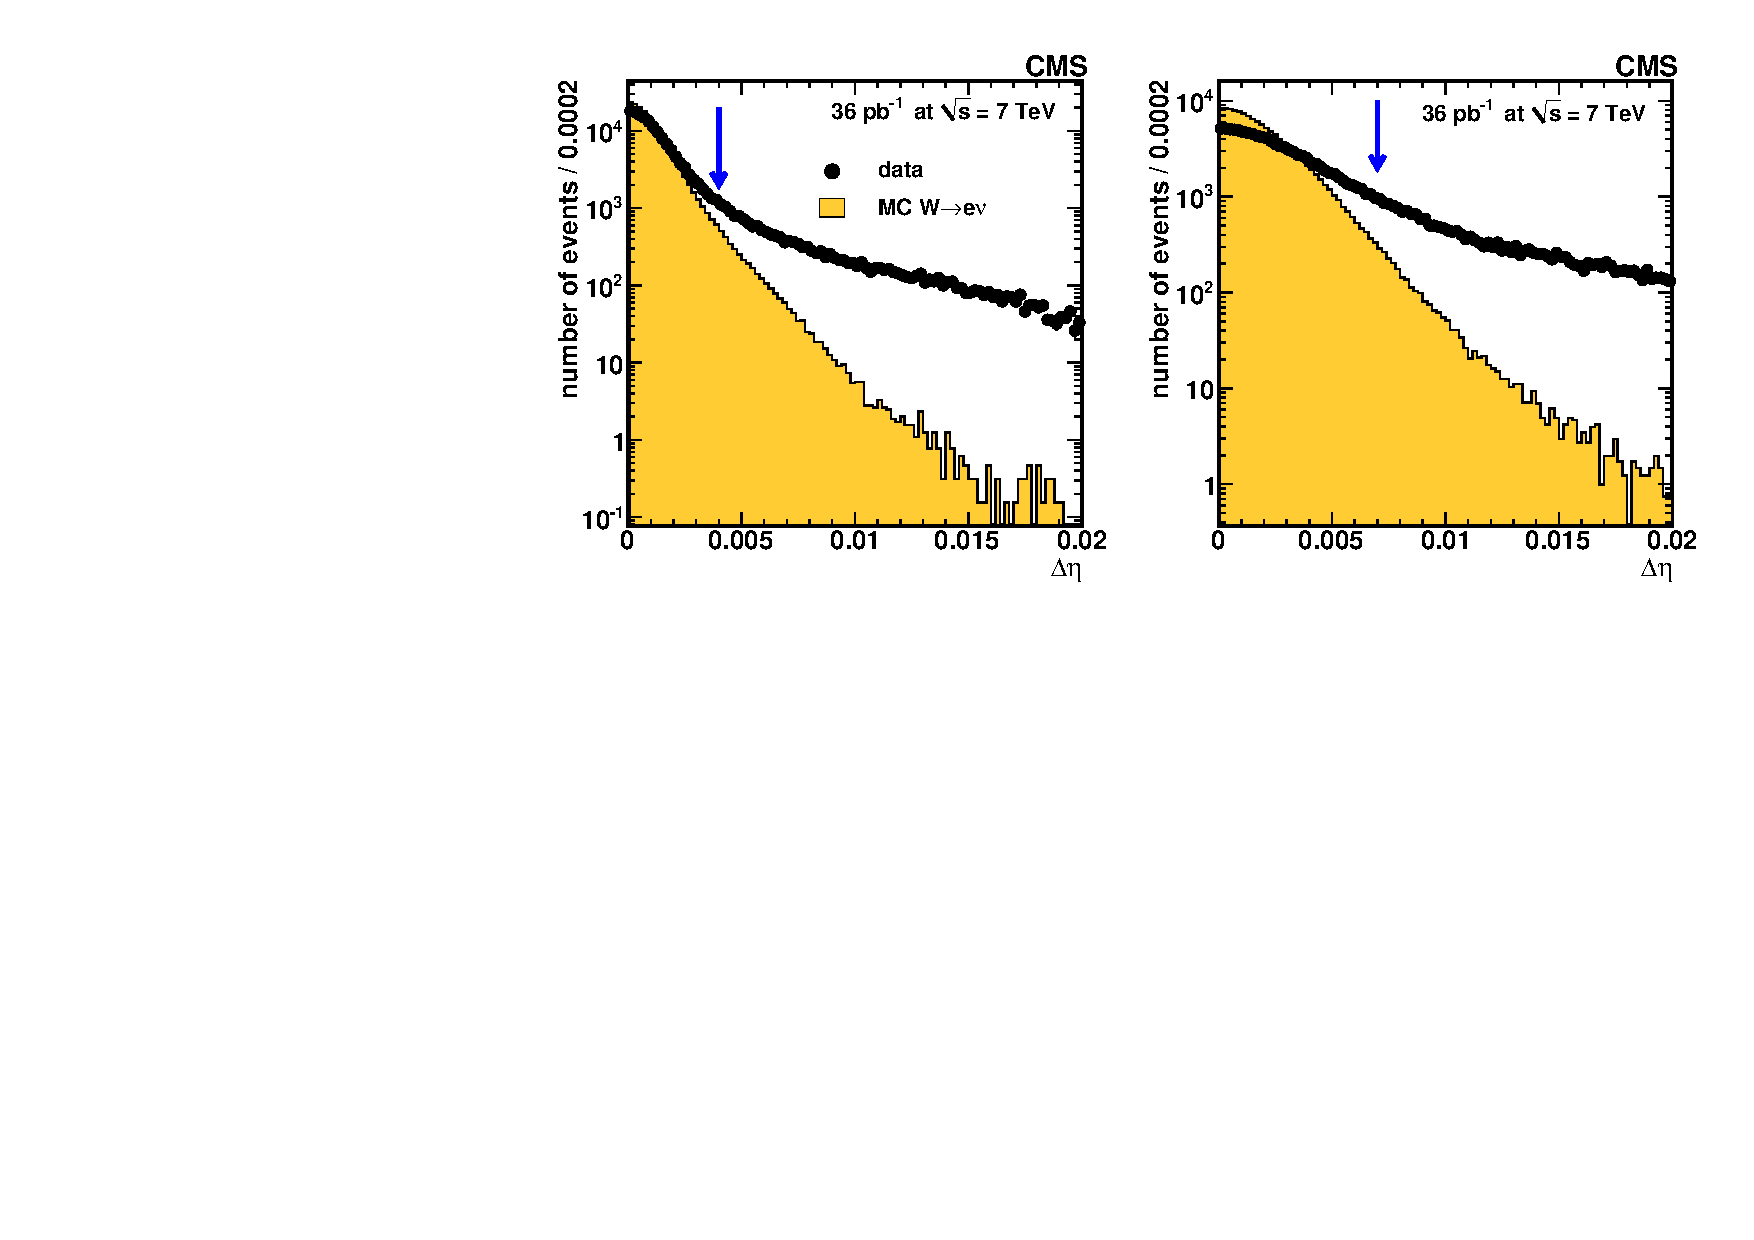
\includegraphics[width=0.68\textwidth]{figs/deta.pdf}
   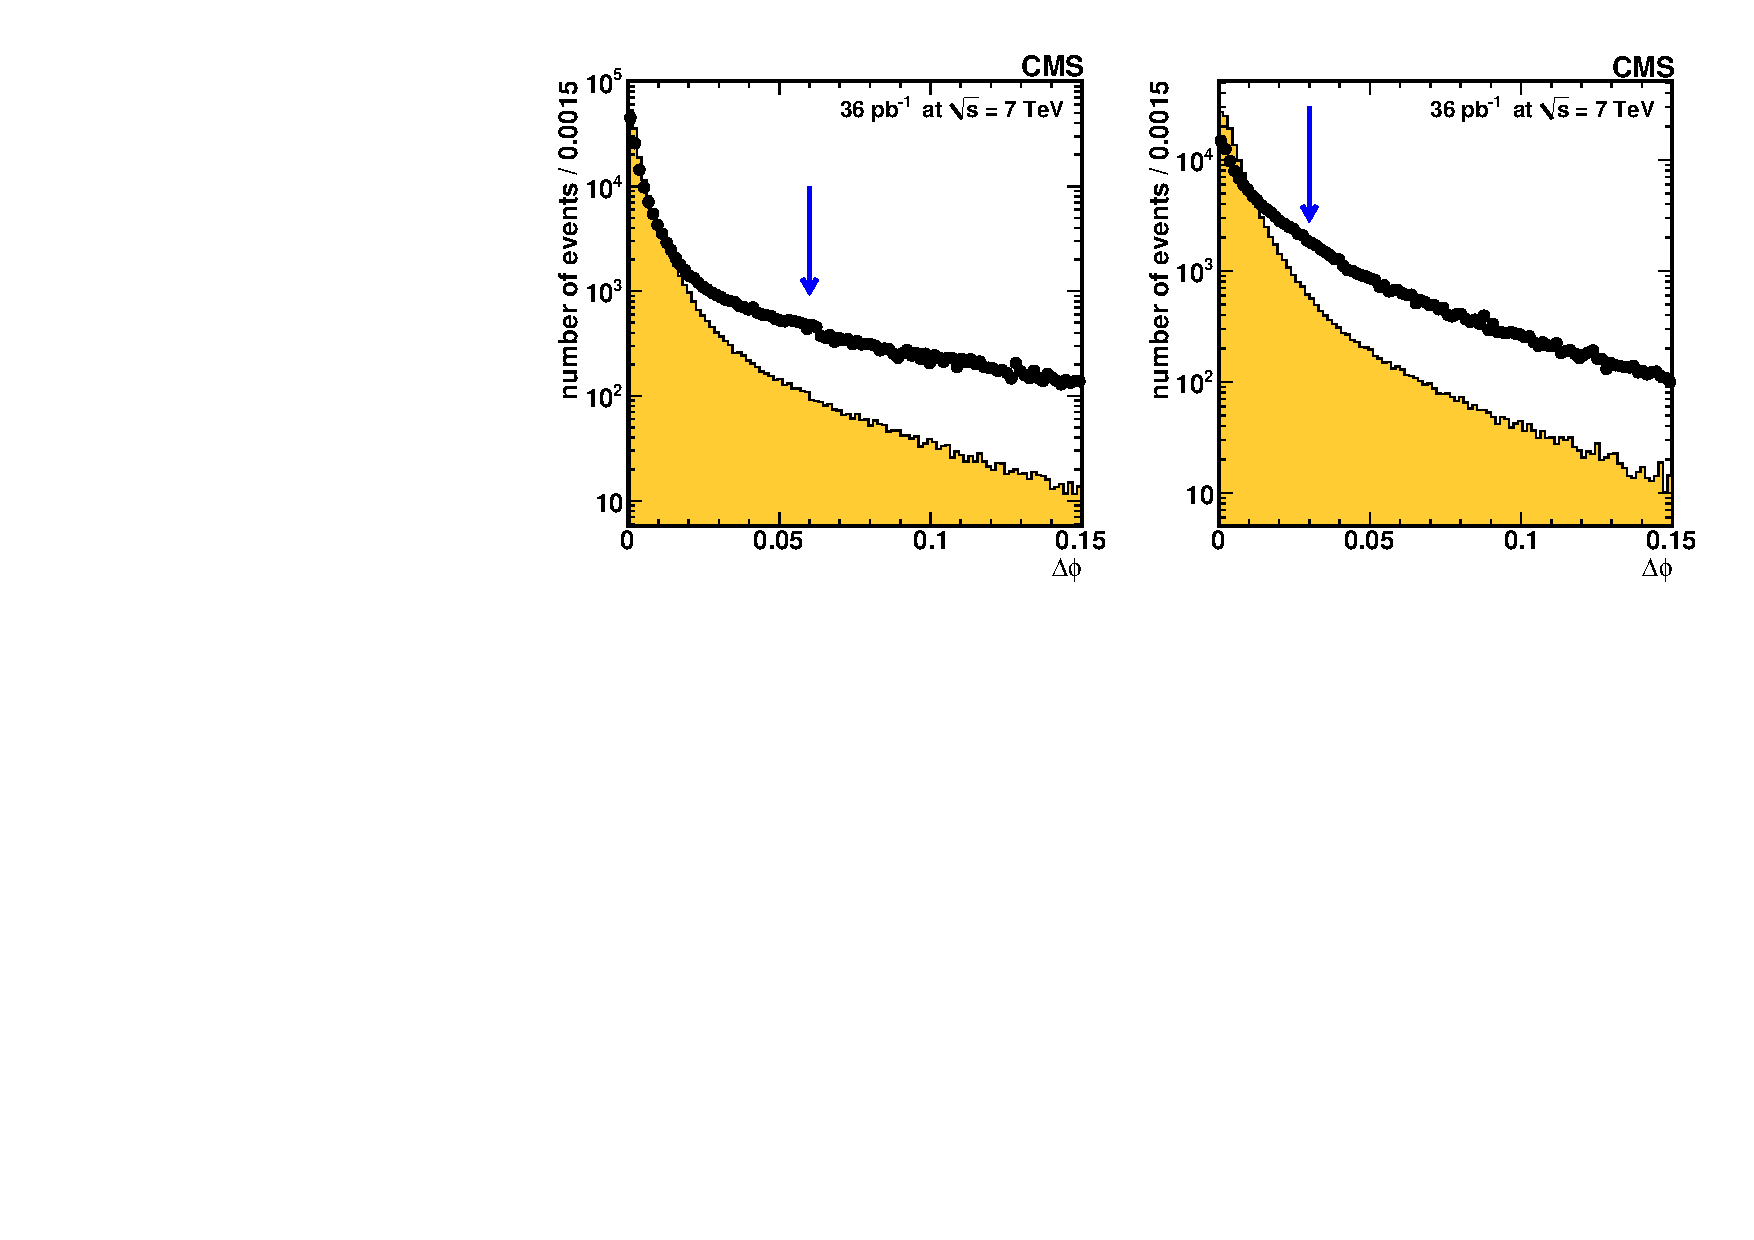
\includegraphics[width=0.68\textwidth]{figs/dphi.pdf}
   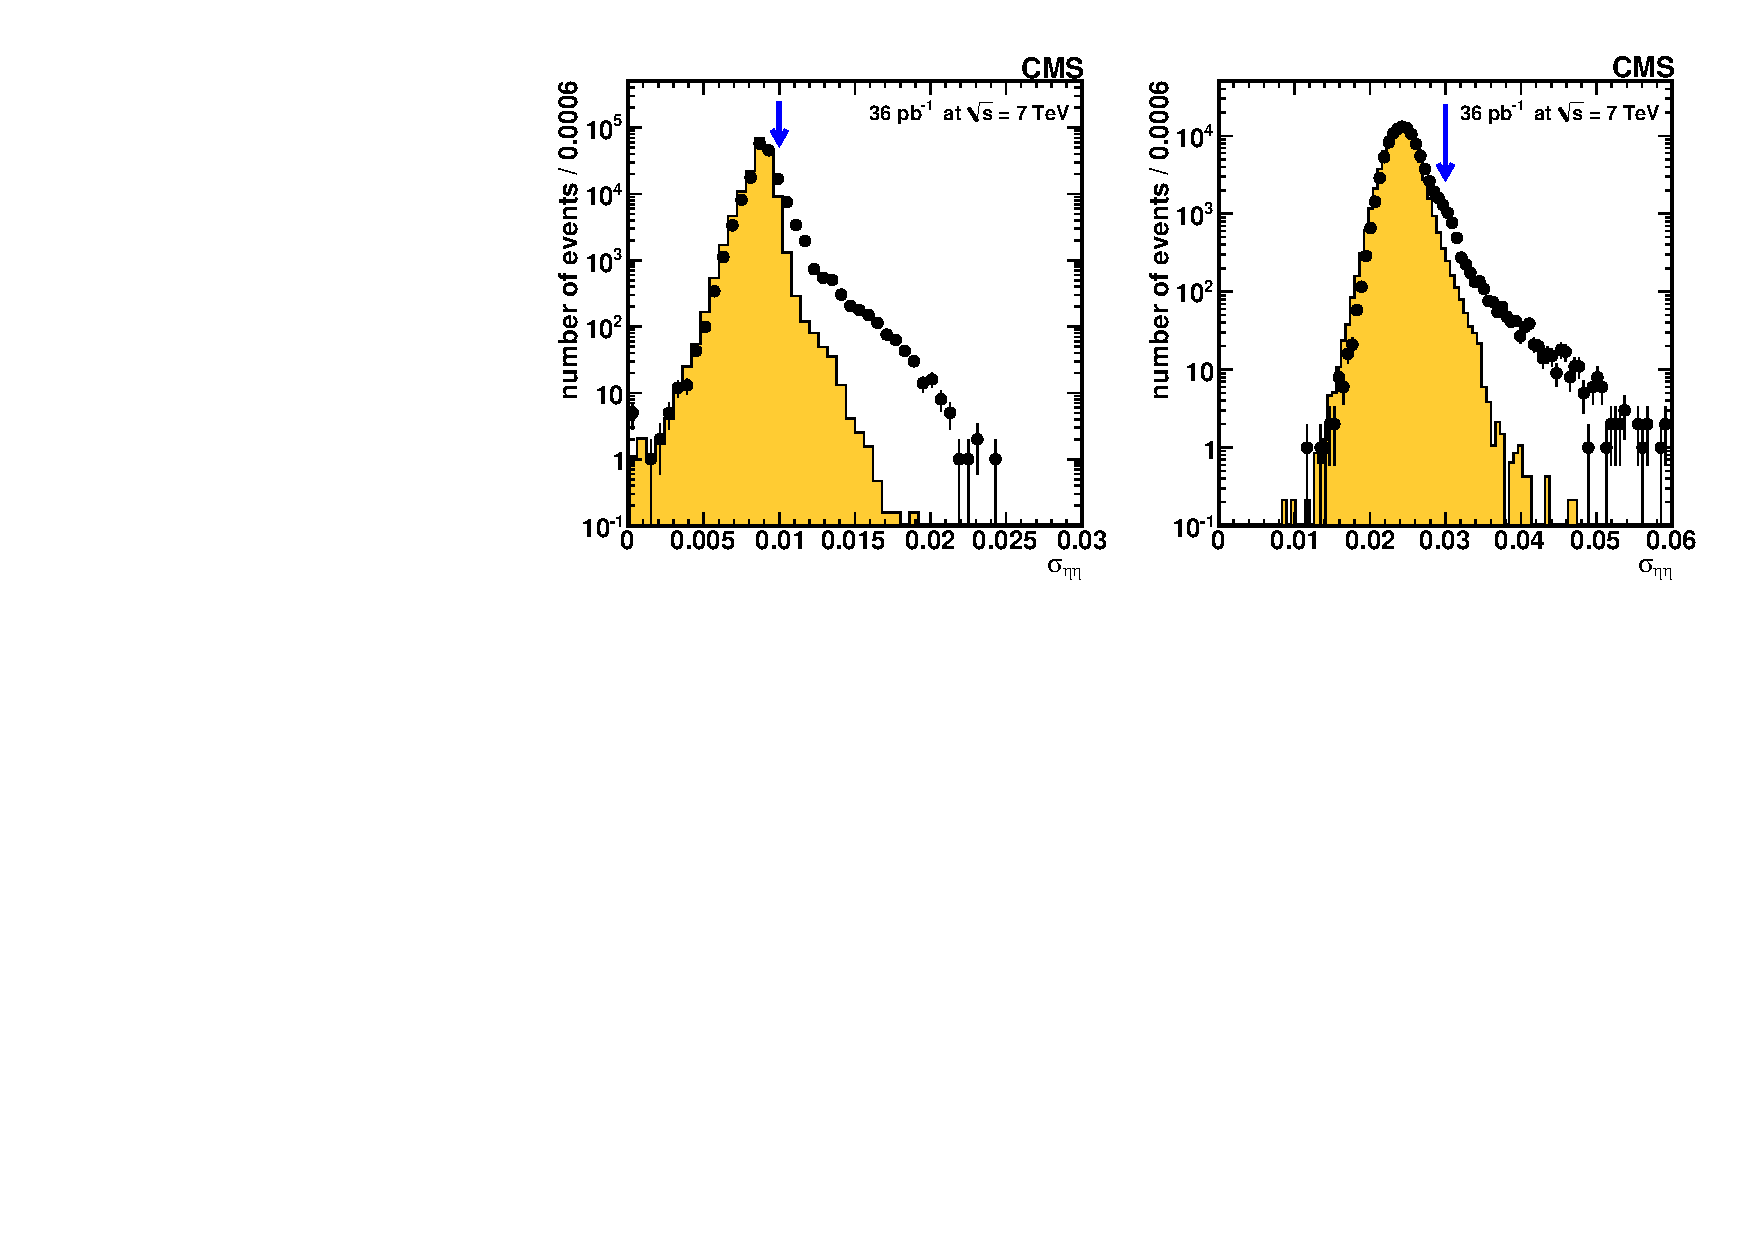
\includegraphics[width=0.68\textwidth]{figs/sihih.pdf}
   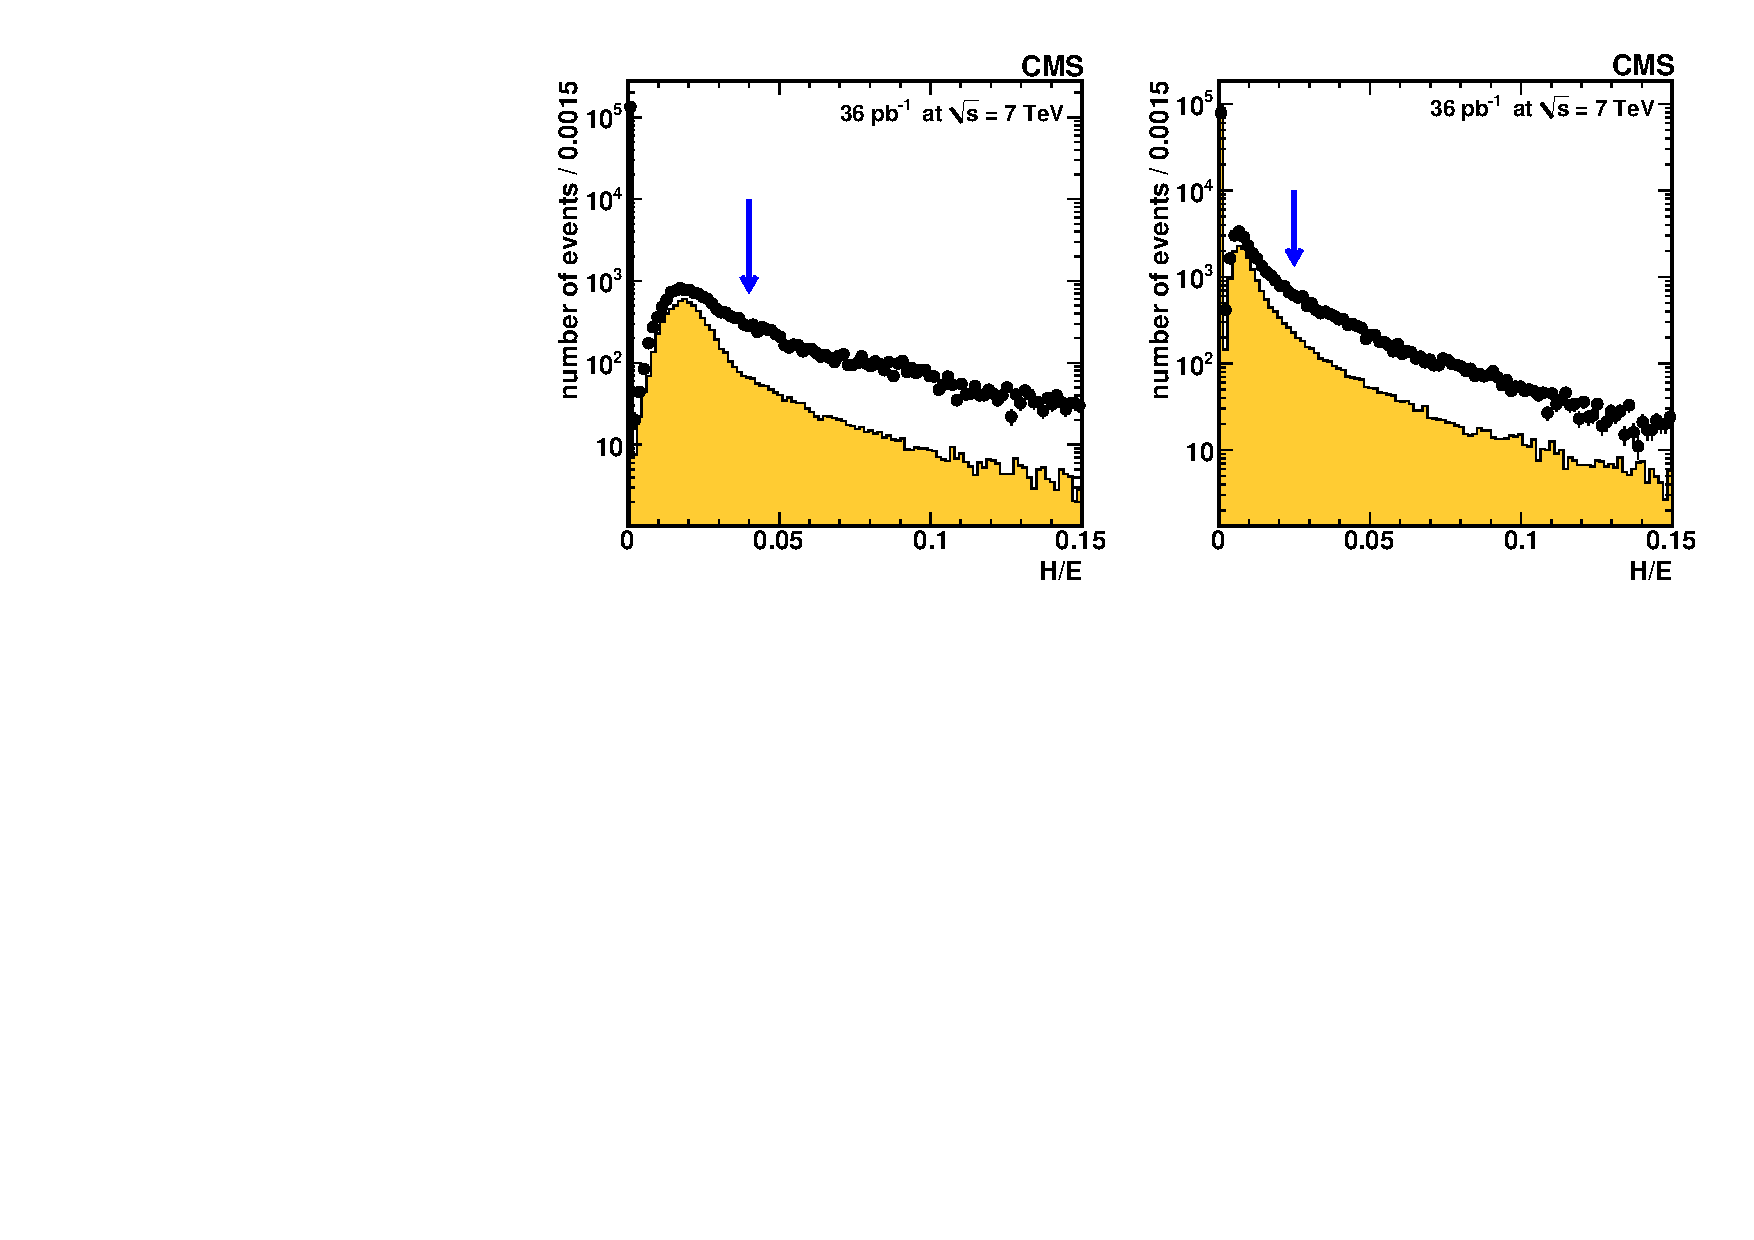
\includegraphics[width=0.68\textwidth]{figs/hoe.pdf}
   \caption{ \label{fig:WenuSelection1}
Distributions of the electron identification variables $\Delta\eta$, $\Delta\phi$, $\sigma_{\eta\eta}$, 
and $H/E$ for data (points with the error bars), for EB (left) and EE (right).
For illustration the simulated $\Wen$ signal (histograms), normalized to the number of events
observed in data, is superimposed.
These distributions are obtained after applying all 
the tight requirements on the selection variables, except that on the presented
variable. The tight requirement on that variable is indicated with an arrow. }
  \end{center}
\end{figure}
%%%%%

%%%%%
\begin{figure}[htbp]
  \begin{center}
   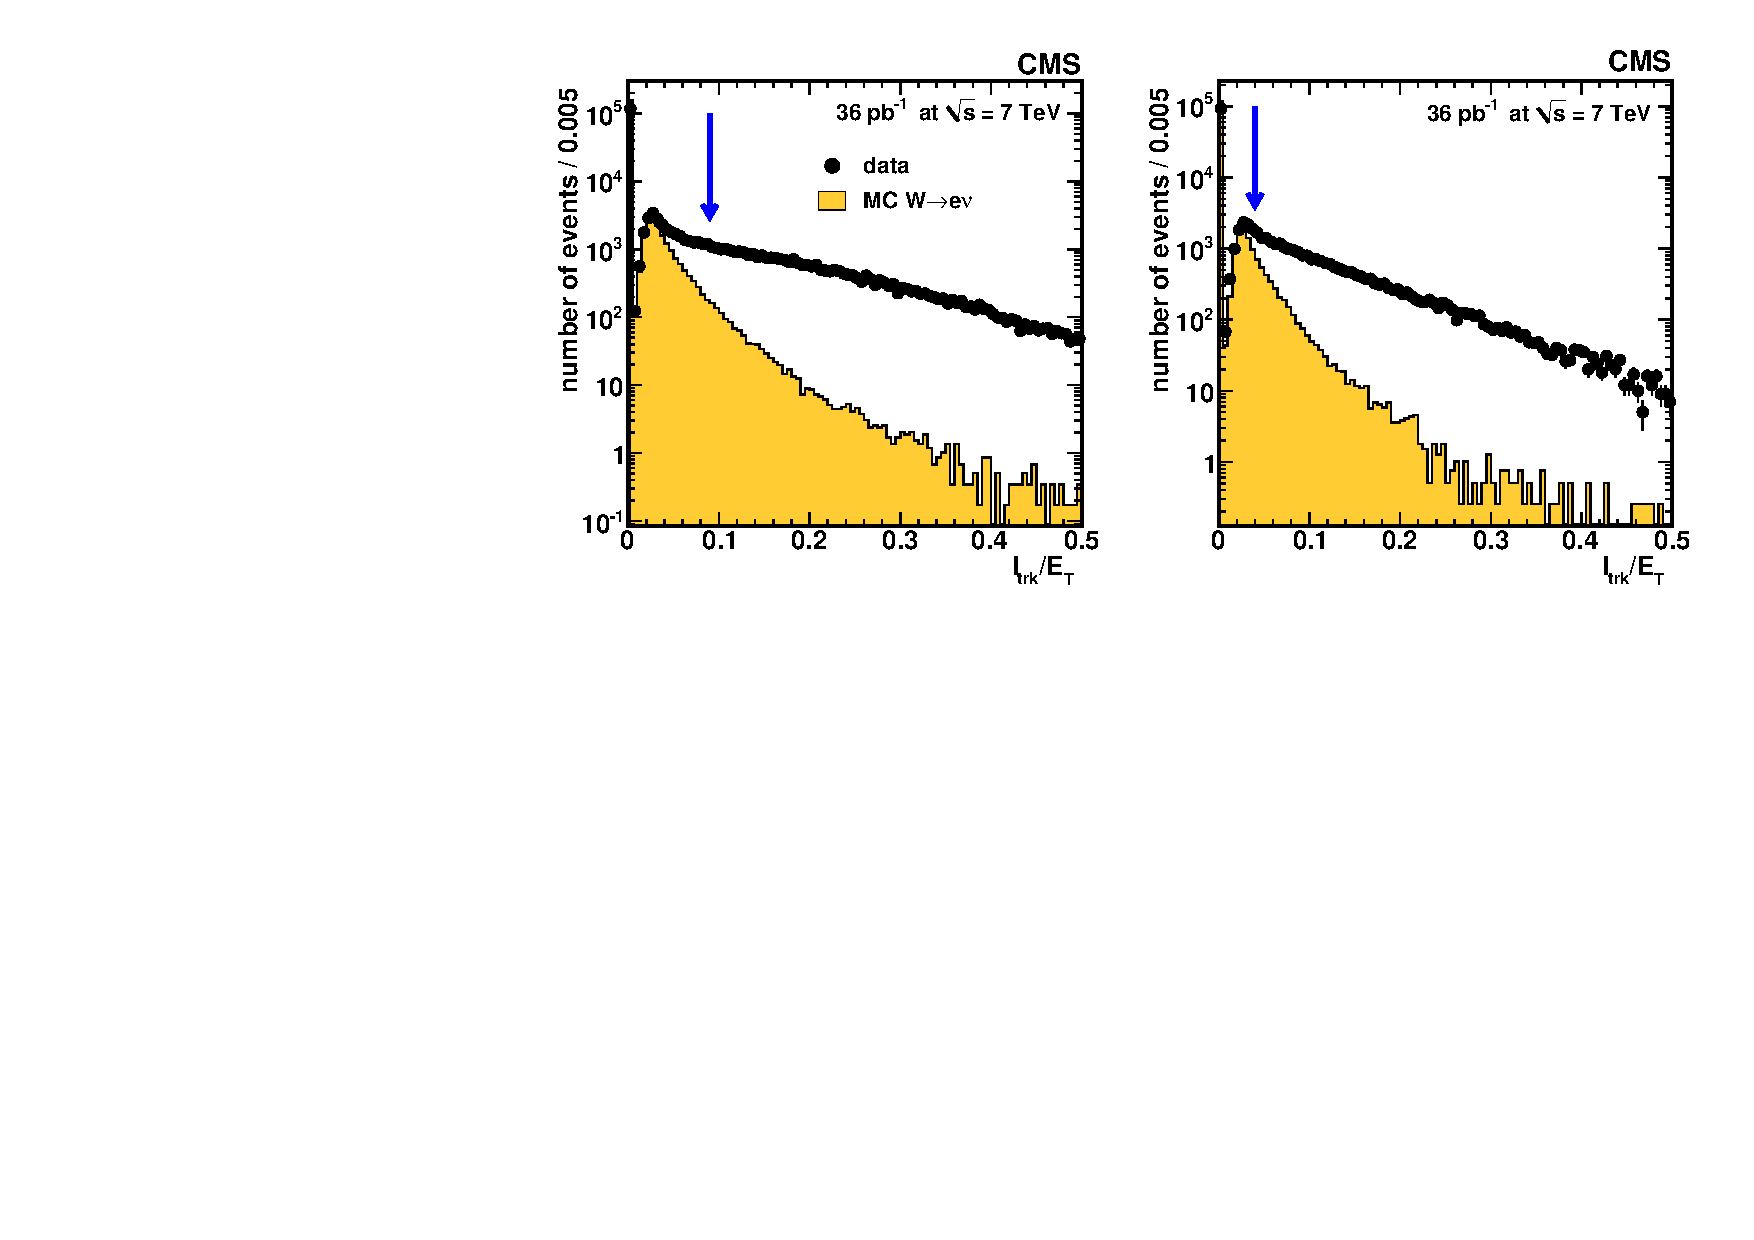
\includegraphics[width=0.68\textwidth]{figs/tkiso.pdf}
   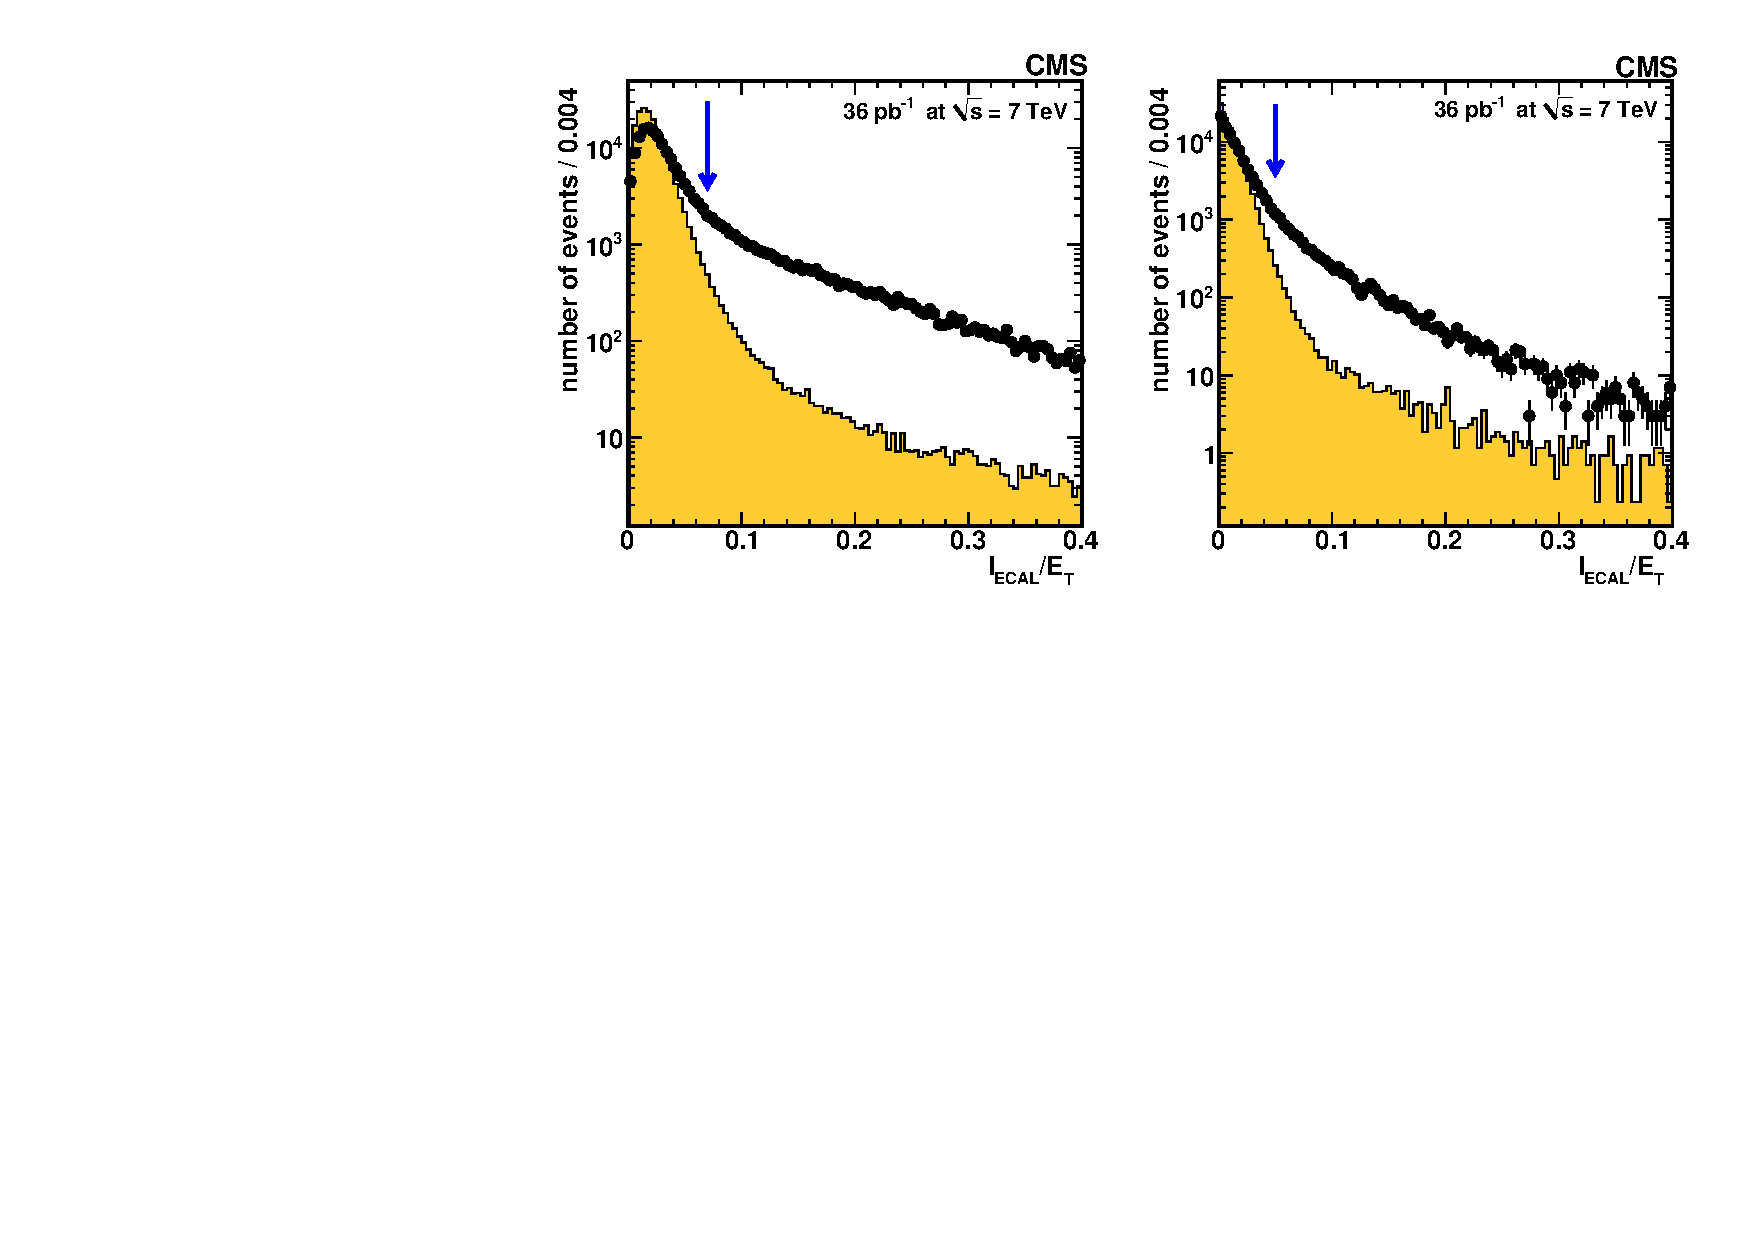
\includegraphics[width=0.68\textwidth]{figs/ecaliso.pdf}
   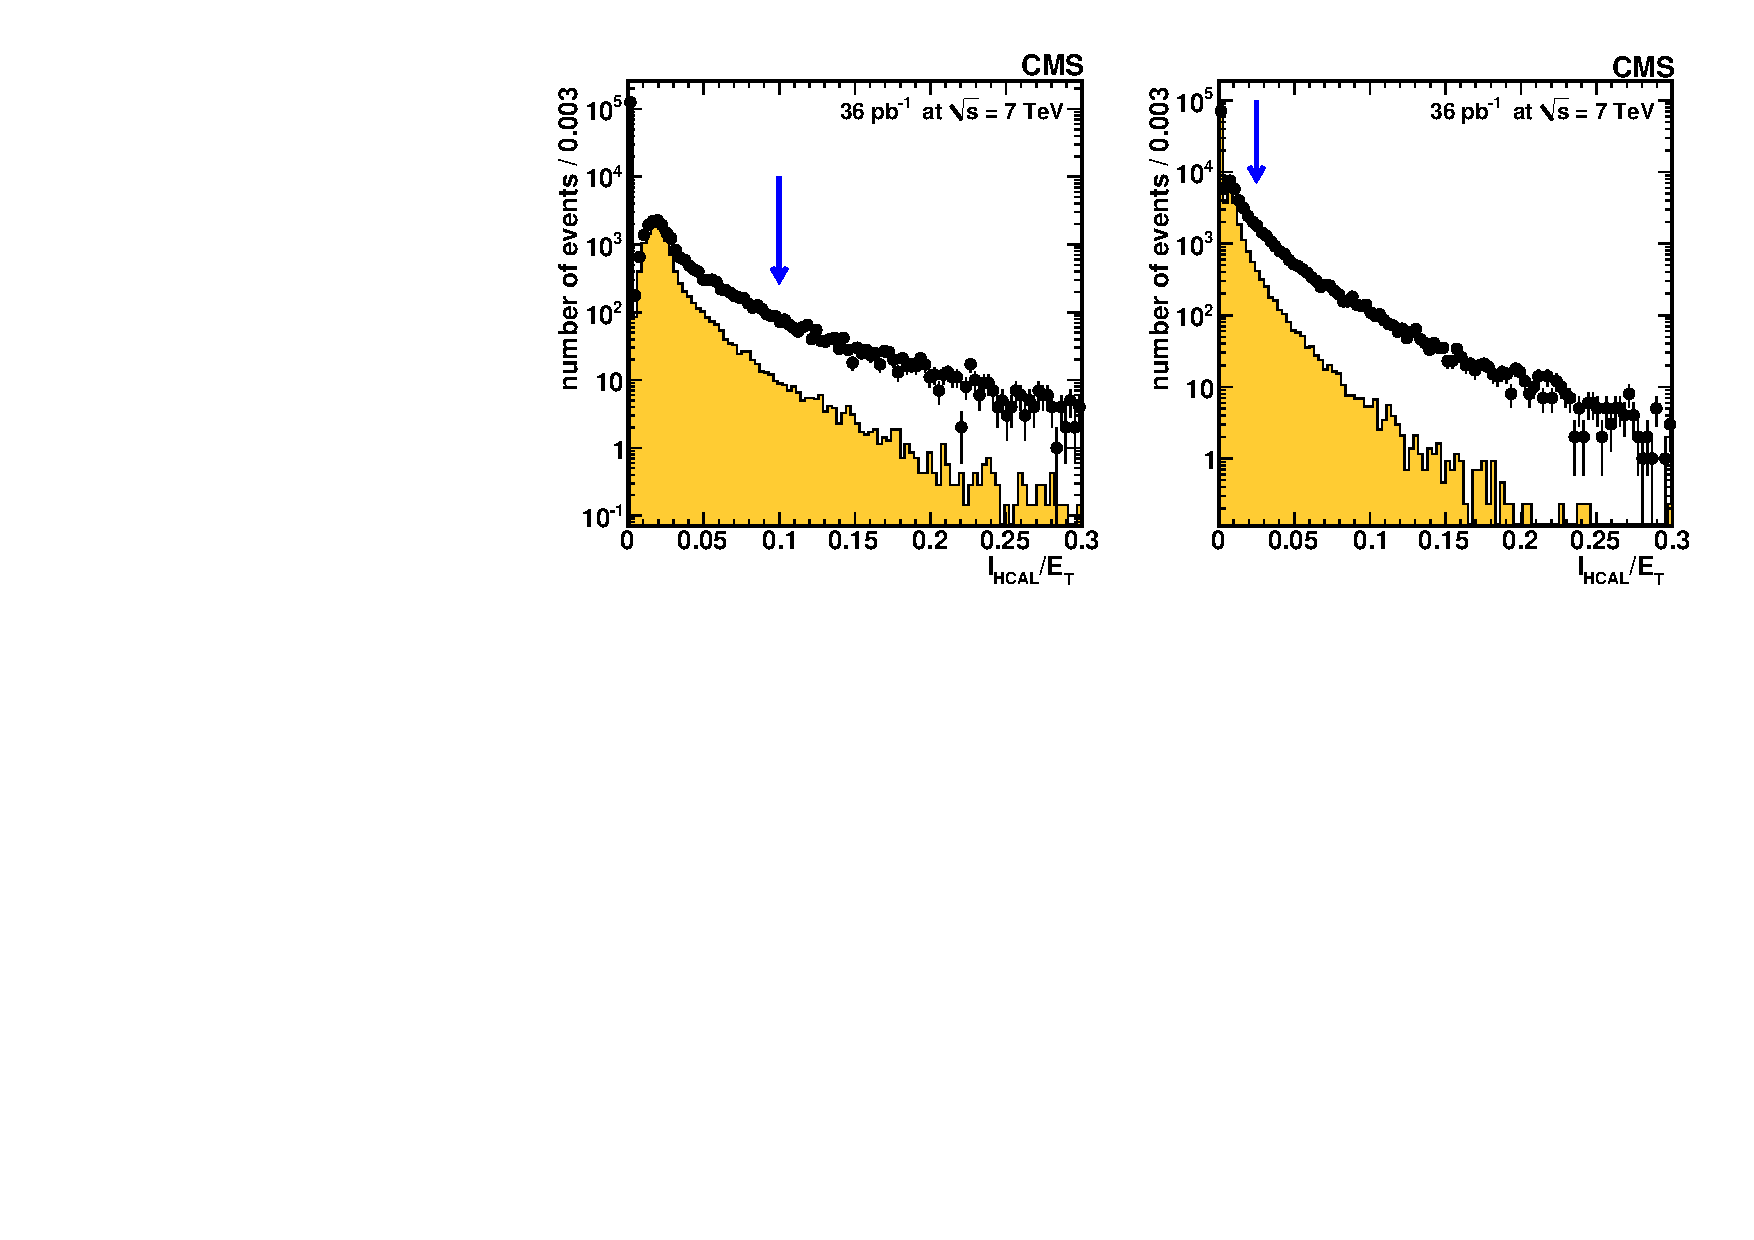
\includegraphics[width=0.68\textwidth]{figs/hcaliso.pdf}
   \caption{ \label{fig:WenuSelection2}
Distributions of the electron isolation variables $\ITRK/\Et$, $\IECAL/\Et$, and $\IHCAL/\Et$
for data (points with the error bars), for EB (left) and EE (right).
For illustration the simulated $\Wen$ signal (histograms), normalized to the number of events
observed in data, is superimposed.
These distributions are obtained after applying all
the tight requirements on the selection variables, except that on the presented
variable. The tight requirement on that variable is indicated with an arrow. }
  \end{center}
\end{figure}
%%%%%

The radiated photons may convert close to the
original electron trajectory, leading to charge misidentification.
Three different methods are used to determine the electron charge. First, the electron 
charge is determined by the signed curvature of the associated GSF track. Second, the charge 
is determined from the associated trajectory reconstructed in the silicon tracker using a 
Kalman Filter algorithm~\cite{KF}. Third, the electron charge is determined based on the azimuthal 
angle between the vector joining the nominal interaction point and the ECAL cluster 
position and the vector joining the nominal interaction point and innermost hit of the GSF track. 
The electron charge is determined from the two out of three charge estimates that are in agreement.
The electron charge misidentification rate is measured in data using the $\Zee$ data
sample to be within 0.1$\%$--1.3$\%$ in EB and 1.4$\%$--2.1$\%$ in EE, increasing with
electron pseudorapidity.


Events are selected if they contain one or two electrons having $\Et>25~\gev$ 
for the $\Wen$ or the $\Zee$ analysis, respectively. 
For the  $\Zee$ selection there is no requirement on the charges of the electrons.
The energy of an electron candidate with $\Et>25~\gev$ is 
determined by the ECAL cluster energy, while its momentum direction is determined by 
that of the associated track. 

Particles misidentified as electrons are suppressed by requiring that the $\eta$ and $\phi$ coordinates
of the track trajectory extrapolated to the ECAL match those
of the ECAL cluster permitting only small differences ($\Delta\eta$, $\Delta\phi$) 
between the coordinates, by requiring a narrow ECAL cluster width in $\eta$ ($\sigma_{\eta\eta}$), 
and by limiting the ratio of the hadronic energy $H$ to the electromagnetic 
energy $E$ measured in a cone of $\Delta R = 0.15$ around the ECAL cluster direction.
More details on the electron identification variables can be found in Refs.~\cite{EGMid,PhotonQCD}. 
Electron isolation is based on requirements on the three isolation 
variables $\IHCAL/\Et$, $\IECAL/\Et$, and $\ITRK/\Et$.

\par
Electrons from photon conversions are suppressed by requiring the 
reconstructed electron track to have at least one hit in the innermost pixel layer.
Furthermore, electrons are
rejected when a partner track is found that is consistent with a
photon conversion, based on the opening angle and the separation in
the transverse plane at the point where the electron and partner
tracks are parallel.

The electron selection criteria were obtained
by optimizing signal and background levels according to
simulation-based studies. The optimization was done for EB
and EE separately.  

Two sets of electron selection criteria are considered: 
a tight one and a loose one.
Their efficiencies, from simulation studies based on $\Wen$ events, are
approximately 80$\%$ and 95$\%$, respectively. These efficiencies correspond 
to reconstructed electrons within the geometrical and kinematic 
acceptance, which is defined in Section~\ref{sec:acceptance}.  
The tight selection criteria give a purer sample of prompt 
electrons and are used for both the $\Wen$ and $\Zee$ analyses.
The virtue of this choice is to have consistent electron definitions 
for both analyses, simplifying the treatment of systematic 
uncertainties in the $\mathrm{W}/\mathrm{Z}$ ratio measurement. 
In addition, the tight working point, applied to both electrons
in the $\Zee$ analysis, reduces the QCD backgrounds to a negligible level.
%%The values of the cuts for the tight and "loose" selection sets are 
%%listed in Table~\ref{tab:electron_cuts}.
%%%%% GD
Distributions of the selection variables are shown in Figs.~\ref{fig:WenuSelection1}
and~\ref{fig:WenuSelection2}.
The plots show the distribution of data together with the simulated signal 
normalized to the same number of events as the data, after applying all 
the tight requirements on the selection variables except the requirement on the displayed
variable. 
%The tight cut on that variable is shown with a vertical line.



For the W analysis, an event is also rejected if there is a second electron 
that passes the loose selection with $\Et > 20~\gev$. This requirement reduces
the contamination from DY events.  
The number of $\Wen$ candidate events selected in the data sample is 
$\WEISAMPLE$, with $\WEPSAMPLE$ positrons and $\WEMSAMPLE$ electrons.

For the Z analysis, two electrons are required within the ECAL acceptance, 
both with $\Et > 25~\gev$ and both satisfying the tight electron selection. 
Events in the dielectron mass region of $60 < m_{\mathrm{ee}} < 120$~GeV are counted.
These requirements select $\ZEESAMPLE$ events.



% \begin{table}[htb]
% \caption{Selection cuts for electrons.}
% \label{tab:electron_cuts}
% \begin{center}
% \begin{tabular}{ | l || c | c || c | c |}
% \hline
%           & \multicolumn{2}{| c ||}{"Loose" e} & \multicolumn{2}{| c |}{tight e} \\
% \hline
%                          & Barrel & Endcap & Barrel & Endcap \\
% \hline \hline
%    $\ITRK/\Et$             & 0.15   & 0.08   & 0.09   & 0.04   \\
% \hline
%    $\IECAL/\Et$              & 2.0    & 0.06   & 0.07   & 0.05   \\
% \hline
%    $\IHCAL/\Et$              & 0.12   & 0.05   & 0.10   & 0.025  \\
% \hline
%    Missing hits $\leq$    & 1      & 1      & 0      & 0      \\
% \hline
%    Dcot                  & $-$    & $-$    & 0.02   & 0.02   \\
% \hline
%    Dist                  & $-$    & $-$    & 0.02   & 0.02   \\
% \hline
%    $\sigma_{\eta\eta}$   & 0.01   & 0.03   & 0.01   & 0.03   \\
% \hline
%    \DP                    & $-$    & $-$    & 0.06   & 0.03   \\
% \hline
%    \DE                    & 0.007  & 0.01   & 0.004  & 0.007  \\
% \hline
%    $H/E$                  & 0.15   & 0.07   & 0.04   & 0.025  \\
% \hline
% \end{tabular}
% \end{center}
% \end{table}







%\subsection{Muons \label{sec:muonId}}

%Muon used in this analysis are selected according to the
%quality criteria studies in
%Events with high-$\Pt$ muons are recorded online using the Level-1 muon
%trigger and the High-Level Trigger (HLT), which requires muons within $|\eta| < 2.1$ and
%with a thresholds of $\Pt>9 \GeVc$ or $\Pt>15 \GeVc$, according to the running periods. 
Muons must be identified by two different algorithms~\cite{MUONPAS}: one proceeds from 
the inner tracker outwards (``tracker muons''), the other one starts from 
segments in the muon chambers and proceeds inwards (``global muons''). 
Decays in flight of hadrons and punch-through are reducing a cut of $\chi^2/ndof < 10$ 
on a global fit containing tracker and muon detector hits. 
In order to ensure a precise estimate of momentum and impact parameter 
%(the muon momentum resolution is dominated by the inner tracker detector
%for the tranverse momentum range interesting for this measurement)
only tracks with more than 10 hits and at least one hit in the pixel detector are used. 
We require at least two levels of muon stations in the measurement, 
to ensures a good quality momentum estimate at trigger level, and
to further suppresses remaining fake muon candidates.
%For the $\Zmm$ analysis we minimize the cross-corrlation between tracker and muon 
%detectors by drop the $\chi^2/{\mathrm{ndof}}$ and 
%the request that the muon is found by the tracker algorithm.
Cosmics are rejected by requiring a transverse impact parameter distance to the beam spot
position of less than 2 mm.



%\subsubsection{$\Wen$}

The event selection requirements for $\Wen$ are then as follows:
\begin{enumerate}
\item
one identified electron within acceptance, satisfying the WP80 set
of identification and isolation criteria,
\item
if a second electron candidate with $\Et > 20~\gev$, within ECAL fiducial 
and satisfying looser identification and isolation criteria (WP95) is present
in the event, the event is rejected.
\end{enumerate}

The number of $\Wen$ candidate events selected
in the data sample is
$\WEISAMPLE$, with
$\WEPSAMPLE$ positrons and
$\WEMSAMPLE$ electrons.


%\subsubsection{$\Wmn$ Event Selection}
\label{sec:WmnSel}

% $\Wmn$ events are characterized by a high-$\Pt$, isolated muon,
% together with a significant amount of missing $\Et$, due to the
% presence of a neutrino in the final-state, that escapes undetected.

The first step in the $\Wmn$ candidate selection is to
reject those events having two global muons satisfying: $\Pt(\mu_1) >
20~\GeV$ and $\Pt(\mu_2) > 10~\GeV$, where $\Pt(\mu_1)$ is the
highest muon $\Pt$ and $ \Pt(\mu_2)$ is the second highest muon $\Pt$
in the event, in order to minimize the contamination from DY
events.

Events with a good quality muon, as described in Section~\ref{sec:muonid},
in the fiducial volume $|\eta|<2.1$, and with a transverse momentum
higher than $25~\GeV$ are kept.
Relative combined isolation variable (see Section~\ref{sec:isolation}) is used to evaluate the level of activity around the
muon. Isolation distribution of the experimental data, together with the simulation expectations, is shown in
Fig.~\ref{figure:Wmunu_iso}. The muon is considered to be isolated if $\IRelComb < 0.1$.
Events with $\IRelComb > 0.2$ are mainly coming from QCD background, and are be used as 
control sample (see Section~\ref{sec:WQCDbkg}).

\begin{figure}[htb] {\centering
    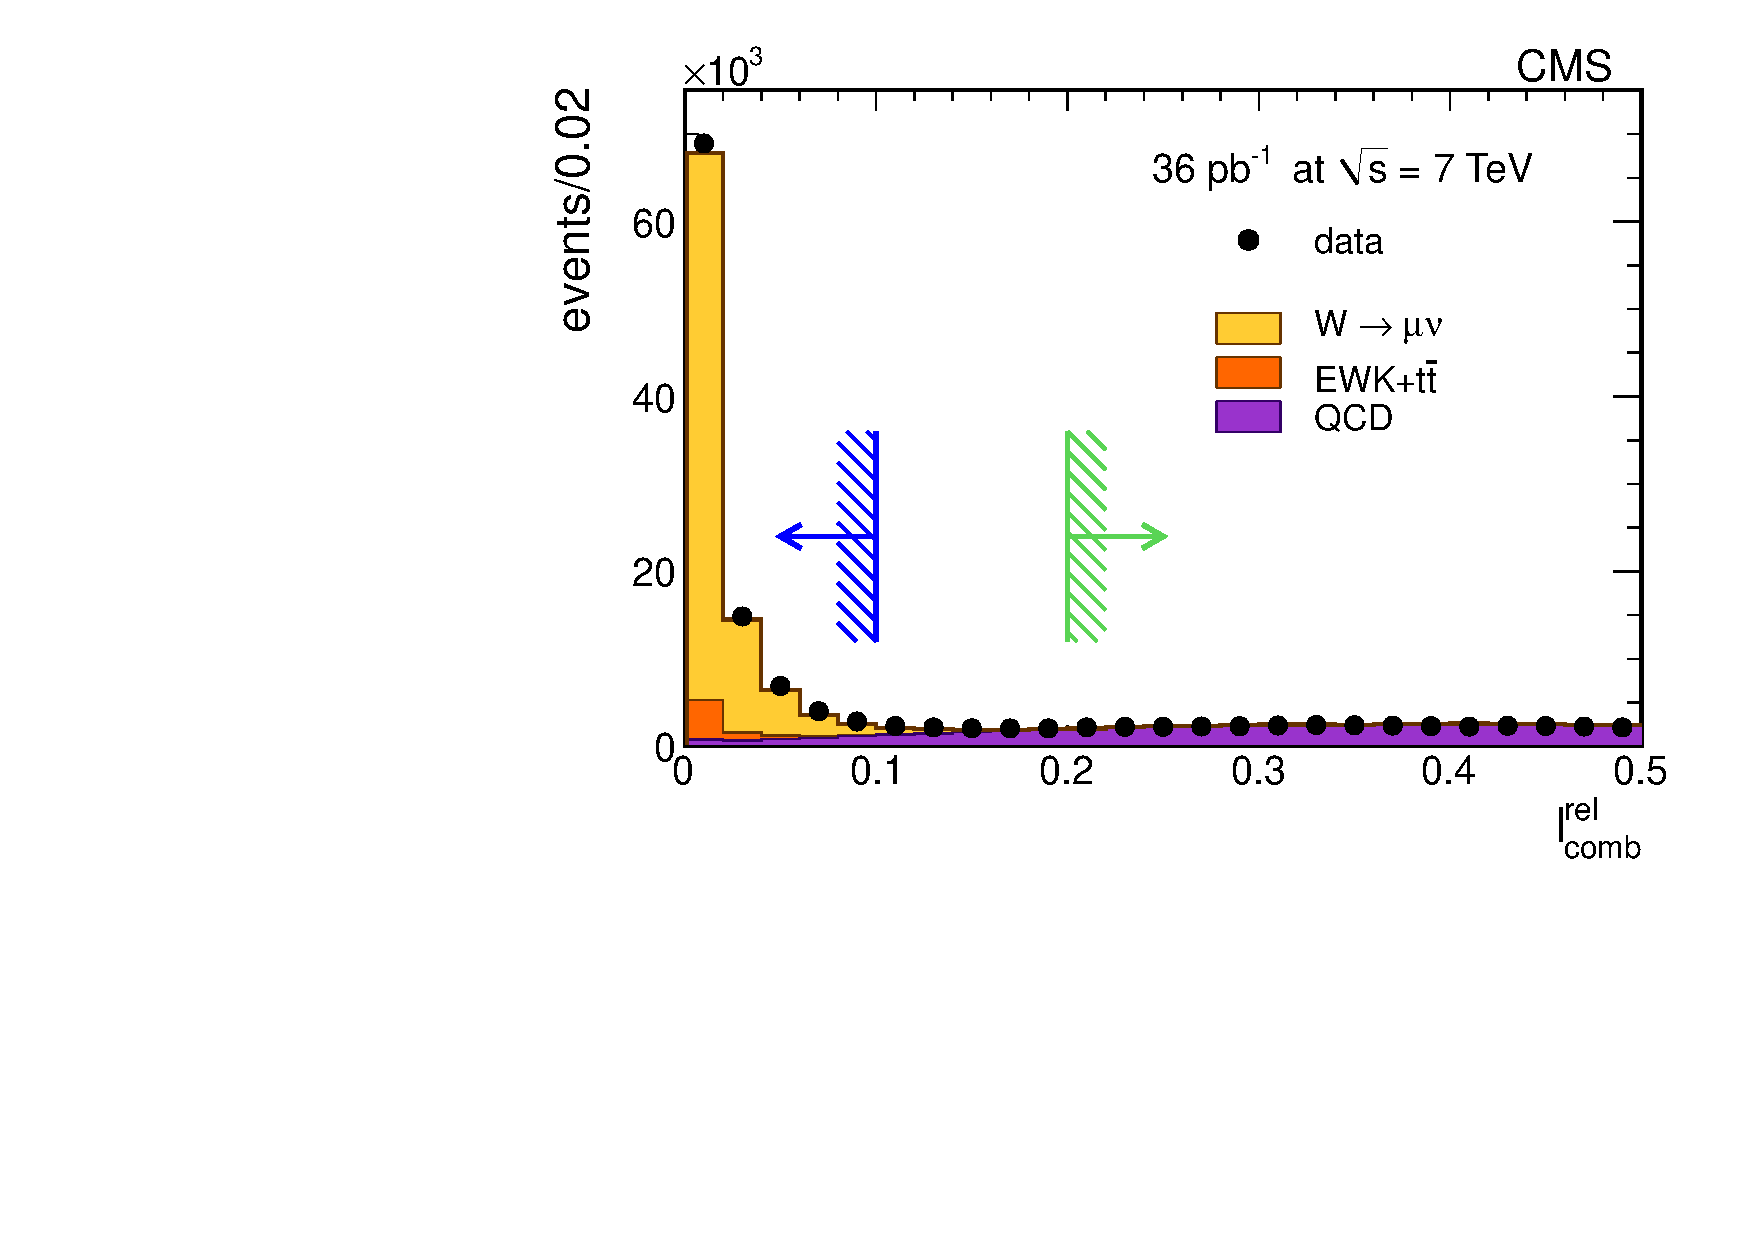
\includegraphics[width=8cm]{figs/Wmunu_isolation.pdf}
    \caption{Isolation distribution of $\Wmn$ candidates with a good quality muon of $\Pt>25~\GeV$ in the fiducial region $|\eta|<2.1$.
Dots represent the data and the solid histograms the contribution from the different SM processes.
The superimposed arrows represent the signal selection requirement (red
arrow, $\IRelComb<0.1$) and selection of the QCD-enriched
control sample (green arrow, $\IRelComb>0.2$).
}
    \label{figure:Wmunu_iso}}
\end{figure}


% The breakdown of the data reduction at the different stages of the
% selection is summarized in Table~\ref{table:Wmunu_selection} both for
% the total sample of muon events, and split by the muon charge.
% %%%%%%%%
% \begin{table}[!ht] 
% \begin{center}
% \begin{tabular}{|c||c|c|c|} \hline
% {Event Sample}                           & Events with $\mu^\pm$ &  Events with $\mu^+$ & Events with $\mu^-$ \\ \hline \hline
% {Candidates}                             &         6395420       &      1812890        &      1677349      \\
% {Triggered}                              &         3174720       &      1644727        &      1529995      \\
% {DY Rejection}                           &         3133420       &       1623994       &      1509425      \\
% {Muon ID}                                &         2618199       &       1346297       &      1271902      \\
% {$|\eta|<2.1$}                           &         2527047       &       1298777       &      1228270      \\
% {$\Pt > 25 \GeV$}                       &          412266       &        222080       &      190186       \\
% $\IRelComb<0.1$                         &          166457       &         97533       &       68924       \\ \hline
% \end{tabular}
% \caption{Data reduction at every step of the selection process.
% Number of events are given for the whole muon data sample, as well as separated by the muon charge.}
% \label{table:Wmunu_selection}
% \end{center}
% \end{table}

After the selection process just described, 166457 events are selected,
97533 of them with a positive charged muon and 68924 with a negative
charged muon.



%\subsection{$\Zll$ Selection}

%
\subsubsection{$\Zee$}


The event selection requirements for $\Zee$ are as follows:
\begin{enumerate}
\item
two electrons within acceptance (as defined above, in Section~\ref{sec:electronId}),
satisfying the WP80 selection,
\item
the dielectron mass must satisfy $60 < m_{\mathrm{ee}} < 120$~GeV.
\end{enumerate}
\par
There is no requirement on the charges of the electrons.
These requirements select \ZEESAMPLE events.



%\input{ZmmSel}

\section{Acceptance}
\label{sec:acceptance}

The acceptance $A_\Wo(\mathrm{e})$ for $\Wen$ is defined
as the fraction of simulated $\Wo$ events having an ECAL cluster within
the ECAL fiducial volume with $\Et>25\GeV$.
The ECAL cluster must match the generated electron after final-state radiation
(FSR) within a cone of $\Delta R=0.2$. No matching in energy is required.

%These acceptances are reported in Table~\ref{tab:e-Waecal}.

% \begin{table}[ht]
%   \begin{center}
%   \begin{tabular}{|l|c|c|c|}
%     \hline
%     $A^{\textrm{ECAL}}_\Wo$  & $\Wp$ & $\Wm$ & $\Wpm$ \\
%     \hline\hline
%     EB     & \WEPEBACC & \WEMEBACC & \WEIEBACC \\
%     EE     & \WEPEEACC & \WEMEEACC & \WEIEEACC \\
%     \hline
%     EB+EE  & \WEPACC & \WEMACC & \WEIACC \\
%     \hline
%     \end{tabular}
%   \end{center}
%   \caption{ ECAL acceptances computed from the POWHEG $\Wen$ samples.
%   \label{tab:e-Waecal}}
% \end{table}

There is an inefficiency in the ECAL cluster reconstruction for
electrons direction within the ECAL fiducial volume
due to a small fraction ($0.5\%$) of noisy or malfunctioning towers
removed from the reconstruction. These are
taken into account in the MC simulation, and no uncertainty is assigned to
this purely geometrical inefficiency. The ECAL cluster selection efficiency is
also affected by a bias in the electron energy scale due to
the $25~\GeV$ energy threshold. The related systematic uncertainty is assigned
to the final $\Wo$ and $\Zo$ selection efficiencies.

The acceptance for the $\Zee$ selection, $A_\Zo(\mathrm{e})$,
is defined as the number of simulated events with
two ECAL clusters  with $\Et>25~\GeV$ within the ECAL fiducial volume and
with invariant mass in the range $60<m_{\mathrm{ee}}<120\,\mathrm{GeV}$, divided by the total number
of signal events in the same mass range, with the invariant mass evaluated using
the momenta at generator level before FSR.
The ECAL clusters must match the two simulated electrons after FSR
within cones of $\Delta R<0.2$. No requirement on energy matching is applied.

For the $\Wmn$ analysis, the acceptance $A_\Wo(\mu)$ is defined as the fraction
of simulated $\Wo$ signal events with muons having transverse momentum $\Pt^{\textrm{gen}}$
and pseudorapidity $\eta^{\textrm{gen}}$, evaluated at the generator level
after FSR, within the kinematic selection: $\Pt^{\textrm{gen}}>25~\GeV$ and $|\eta^{\textrm{gen}}|<2.1$.
% Similarily, for $\Wmn$ the muon is required to have a muon with $p_T^{\textrm{gen}}>25\GeV$
% and $|\eta^{\textrm{gen}}|<2.1$.

The acceptance $A_\Zo(\mu)$ for the $\Zmm$ analysis is defined as the number of
simulated $\Zo$ signal events with both muons passing the kinematic selection with momenta evaluated
after FSR, $\Pt^{\textrm{gen}}>20~\GeV$ and $|\eta^{\textrm{gen}}|<2.1$, and with
invariant mass in the range $60<m_{\mu\mu}<120\,\mathrm{GeV}$, divided by the total number
of signal events in the same mass range, with the invariant mass evaluated using
the momenta at generator level before FSR.

Table~\ref{tab:WZlaccgen} presents the acceptances
for $\Wp$, $\Wm$, and inclusive $\Wo$ and $\Zo$ events,
computed from samples simulated with {\sc powheg} using the CT10 PDF,
for the muon and the electron channels. The acceptances are affected by several
theoretical uncertainties,
which are discussed in detail in Section~\ref{sec:theory}.

\begin{table}[htbp] %
\begin{center}
\caption[.] {\label{tab:WZlaccgen}
Acceptances from {\sc powheg} (with CT10 PDF) for $\Wln$ and $\Zll$ final states,
with the MC statistics uncertainties.\\}
\begin{tabular}{|l|c|c|}
\hline
 {\multirow{2}{*}{Process}} &  \multicolumn{2}{c|}{$A_{\mathrm{W,Z}}$}  \\ \cline{2-3}
  & $\ell=\mathrm{e}$ &$\ell=\mu$ \\
\hline\hline
%      $\Wpln$      & \WEPAGEN & \WMPAGEN \\
%      $\Wmln$      & \WEMAGEN & \WMMAGEN\\
%      $\Wln$  & \WEIAGEN & \WMIAGEN \\
     $\Wpln$      & \WEPACC & \WMPAGEN \\
     $\Wmln$      & \WEMACC & \WMMAGEN\\
     $\Wln$  & \WEIACC & \WMIAGEN \\
\hline
% $\Zll$ & \ZEEAGEN & $0.3977 \pm 0.0017$ \\
$\Zll$ & \ZEEACC & $0.3978 \pm 0.0005$ \\
\hline
\end{tabular}
\end{center}
\end{table}


% \begin{table}[htbp]
%   \begin{center}
%   \begin{tabular}{|l|c|}
%     \hline
%     $A^{\textrm{ECAL}}_\Zo$  & $Z \to e^+e^-$ \\
%     \hline\hline
%     EB+EB     & \ZEEBBACC \\
%     EB+EE     & \ZEEBEACC \\
%     EE+EE     & \ZEEEEACC \\
%     \hline
%     all       & \ZEEACC \\
%     \hline
%     \end{tabular}
%   \end{center}
%   \caption{ Signal acceptances computed from POWHEG $Z \to e^+e^-$ samples.
%   \label{tab:e-Zaecal}}
% \end{table}

\section{Efficiencies}
\label{sec:efficiencies}

A key component of this analysis is the estimation of lepton efficiencies.
The efficiency is determined for different selection steps:
\begin{itemize}
\item offline reconstruction of the lepton;
\item lepton selection, with identification and isolation criteria;
\item trigger (L1+HLT).
\end{itemize}
The order of the above selections steps is important. Lepton efficiency for each
selection is determined with respect to the prior step.
\par
%
% Should we define TNP here and use it afterwards? L.L.
%
A tag-and-probe (\TNP) technique is used, as described below, on pure samples of $\Zll$ events.
The statistical uncertainty on the efficiencies is
ultimately propagated as a systematic uncertainty on the cross-section measurements.
This procedure has the advantage
of extracting the efficiencies from a sample of leptons kinematically very similar
to those used in the $\Wo$ analysis and exploits the relatively pure selection
of $\Zll$ events obtained after a dilepton invariant mass requirement around the Z mass.
\par
The \TNP method is as follows: one lepton candidate,
called the ``tag'', satisfies trigger criteria, tight identification
and isolation requirements. The other lepton candidate, called the ``probe'',
is required to pass specific criteria that depend on the efficiency under study.
\par
For each kind of efficiency, the \TNP method is applied to real data and to
simulated samples, and the ratio of efficiencies in data ($\effdata$) and simulation ($\effmc$) is computed:
\begin{equation}
\label{eq:rho}
 \rhoeff = \frac{\effdata}{\effmc}\,,
\end{equation}
together with the associated statistical and systematic uncertainties.


\subsection{Electrons}
\label{sec:ELEefficiencies}

%The overall electron efficiency is the product of
%three terms: the reconstruction efficiency (GSF tracking),
%the selection efficiency (identification and isolation criteria),
%and the trigger efficiency (L1+HLT), taken in this order.
As mentioned in the previous section, 
the tight electron selection is considered for both the W and Z analyses, so 
the overall efficiency can be written as
\begin{equation}
  \EPS{all} = \EPS{rec}\, \EPS{tight}\, \EPS{trg}.
\label{eq:e-eff}
\end{equation}
The reconstruction efficiency $\EPS{rec}$ is relative to ECAL clusters
within the ECAL acceptance, the selection efficiency $\EPS{tight}$ is relative to GSF electrons
within the acceptance, and the trigger efficiency $\EPS{trg}$ is relative to electrons
satisfying the tight selection criteria.

\par
All the efficiencies are determined by the \TNP technique.
%The tag electron is required to pass the tight electron
%identification criteria. 
Selections with different criteria have been 
tried on the tag electron. It was found that the estimated efficiencies are 
insensitive to the tag selection definition. 
The invariant mass of the \TNP pair
is required to be within the window $60<m_{\mathrm{ee}}<120~\GeV$.
%,ensuring high purity of the probe sample. 
No opposite-charge requirement is enforced.
%The measured efficiency for a given selection
%is the fraction of probes passing the selection.

The number of probes passing and failing the selection is
determined from fits to the invariant mass distribution,
with signal and background components.
Estimated backgrounds, mostly from QCD multijet processes, are in most cases
at the percent level of the overall sample, but can be larger in subsamples
where the probe fails a selection, hence the importance of background
modeling. The signal shape is a Breit--Wigner with nominal Z mass and width convolved with an
asymmetric resolution function (Crystal Ball~\cite{CrystalBall}) with floating parameters.  The
background is modeled by an exponential. Systematic uncertainties that depend on the efficiency
under study are determined by considering alternative signal and background shape models.
Details can be found in Section~\ref{sec:systematics}. 

%A systematic error which depends on the efficiency
%under study is determined by considering alternative background models like power-low or error function
%multiplied with an exponential. The size of the background systematic is 0.3$\%$ for the electron
%identification efficiencies and 1.0$\%$ for electron reconstruction efficiency. The estimation
%of the trigger efficiency is considered to be background free.

%
% GD too technical to be interesting
%
%For this selection, only the charge of the probe is considered except for the
%determination of the reconstruction efficiency, where the probe (which is an
%ECAL cluster) is assigned the charge opposite to that of the tag.
%For the determination of the reconstruction efficiency,
%the probe is an ECAL cluster within ECAL acceptance.
%To reduce the background level, and only in that case, we
%require the ECAL cluster to pass a loose $H/E<0.15$ 
%requirement for both EB and EE which is shown from
%simulations to be almost uncorrelated with the reconstruction efficiency.
%The reconstruction efficiencies have been independently estimated by varying 
%the ECAL cluster "cleaning" criteria or without any cleaning cuts giving 
%consistent results with the first method.


%\begin{figure}[htbp]
%\begin{center}
% \begin{minipage}[Reconstruction]{0.32\textwidth}
%  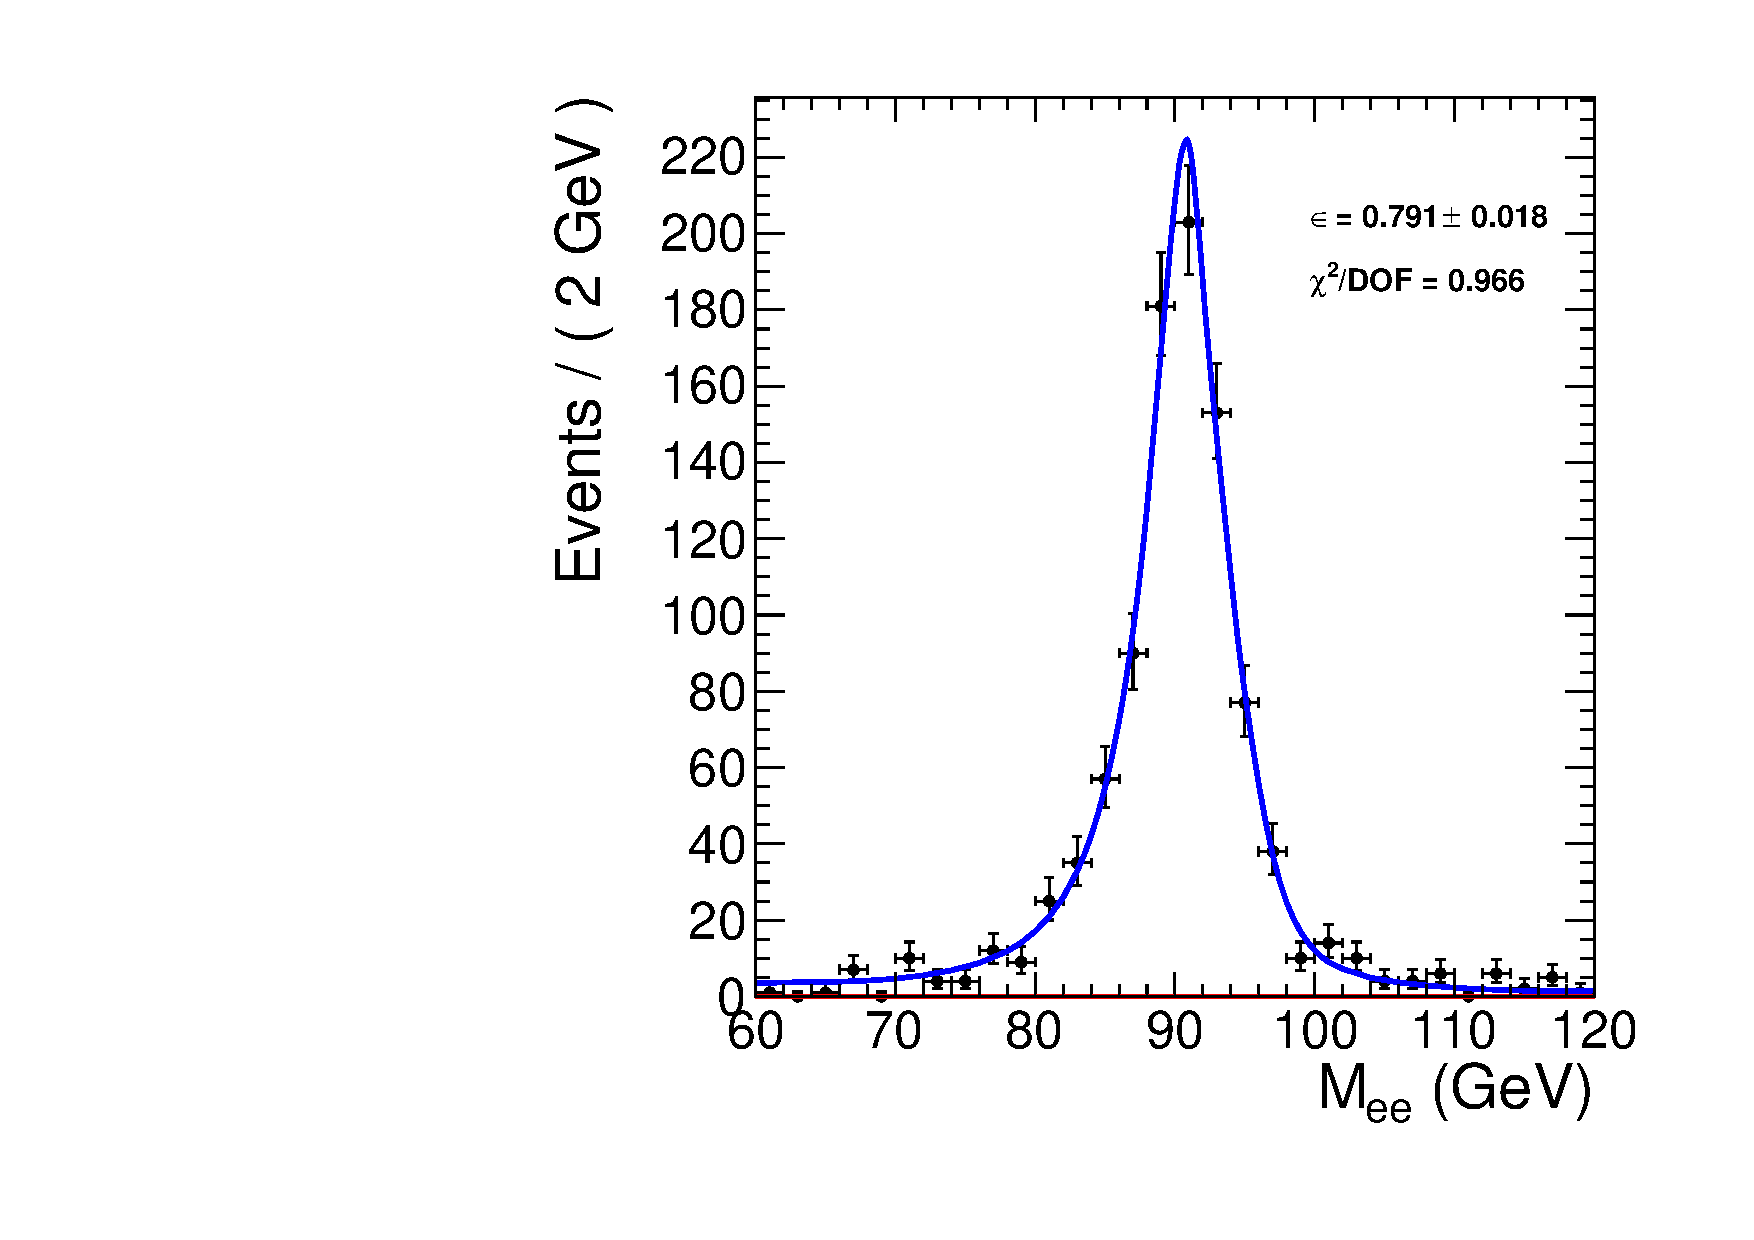
\includegraphics[width=1.0\textwidth]{figs/tpHistos_ID80_eb_pass.pdf}
%  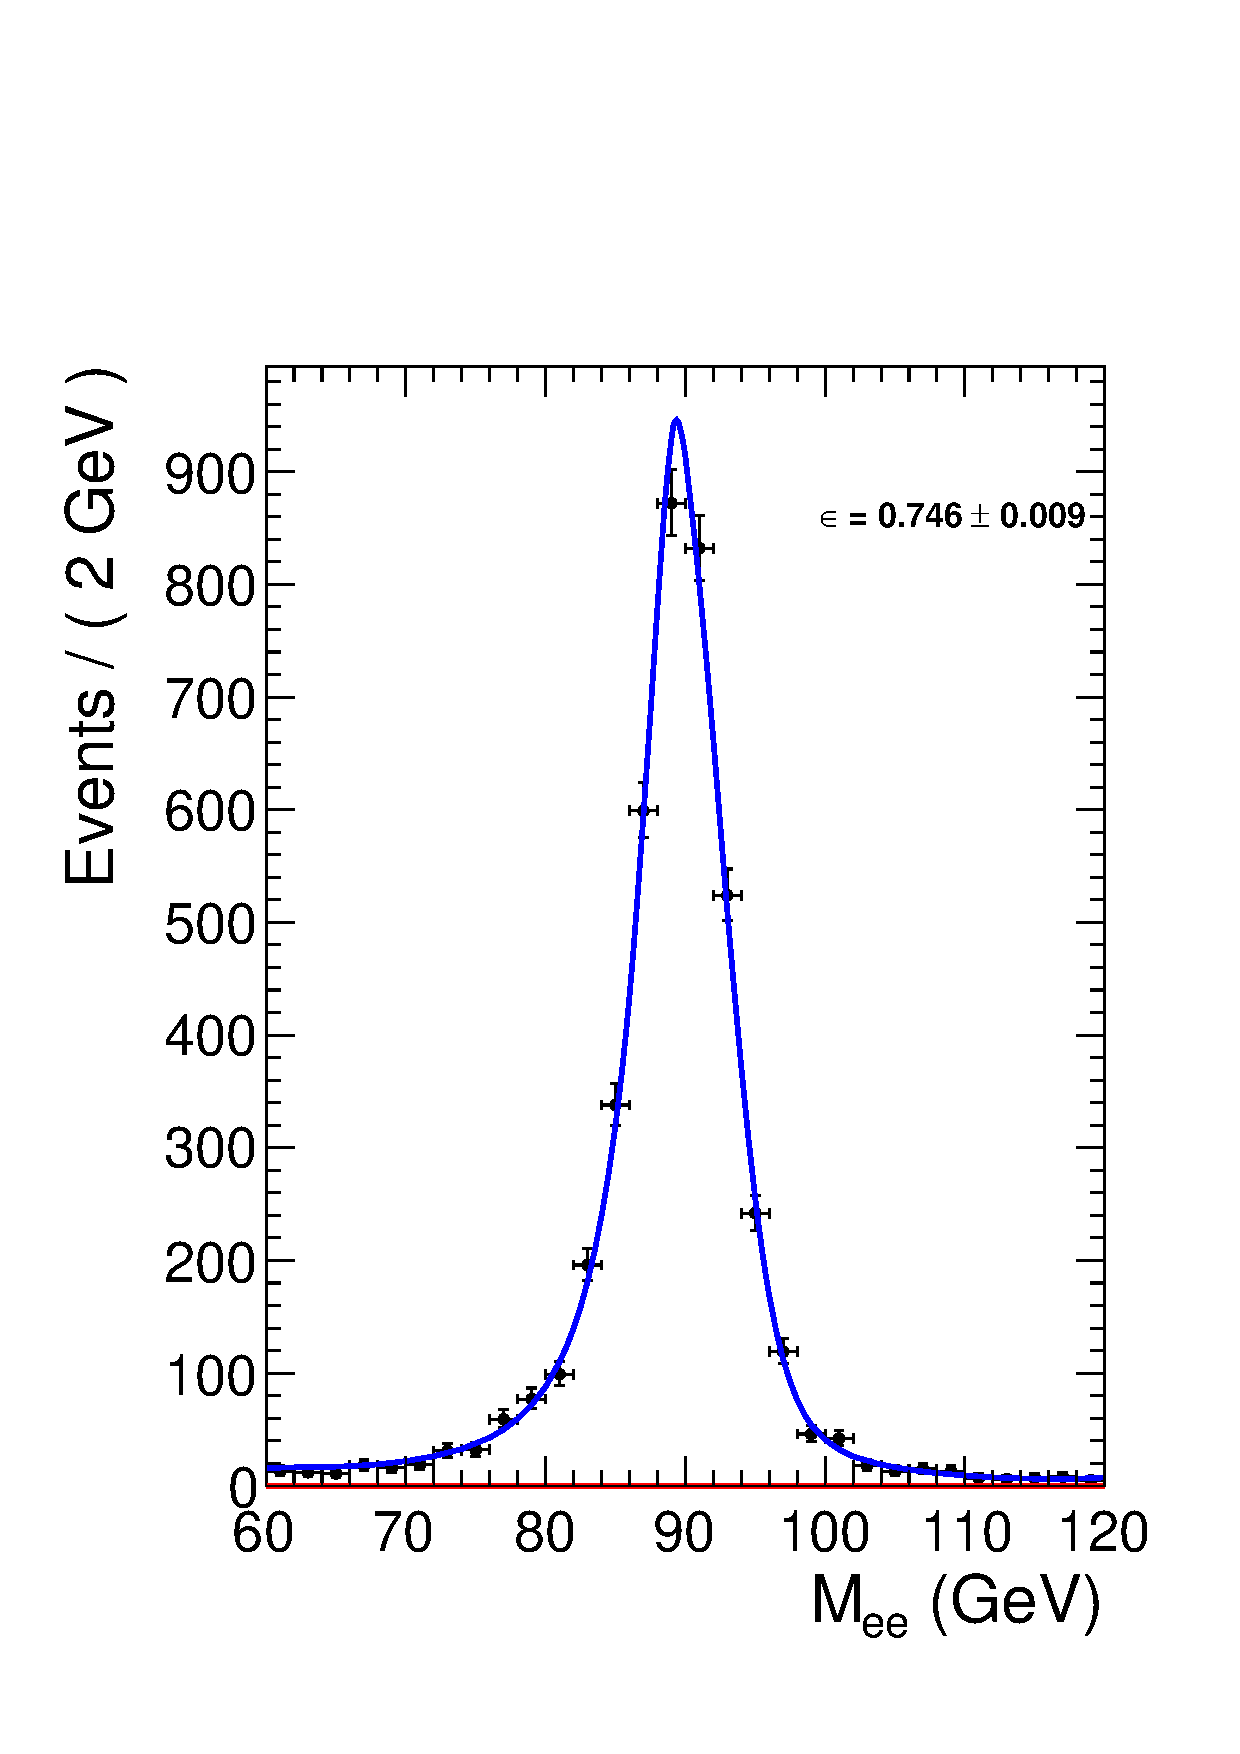
\includegraphics[width=1.0\textwidth]{figs/tpHistos_ID80_ee_pass.pdf}
% \end{minipage}
% \begin{minipage}[WP80]{0.32\textwidth}
%  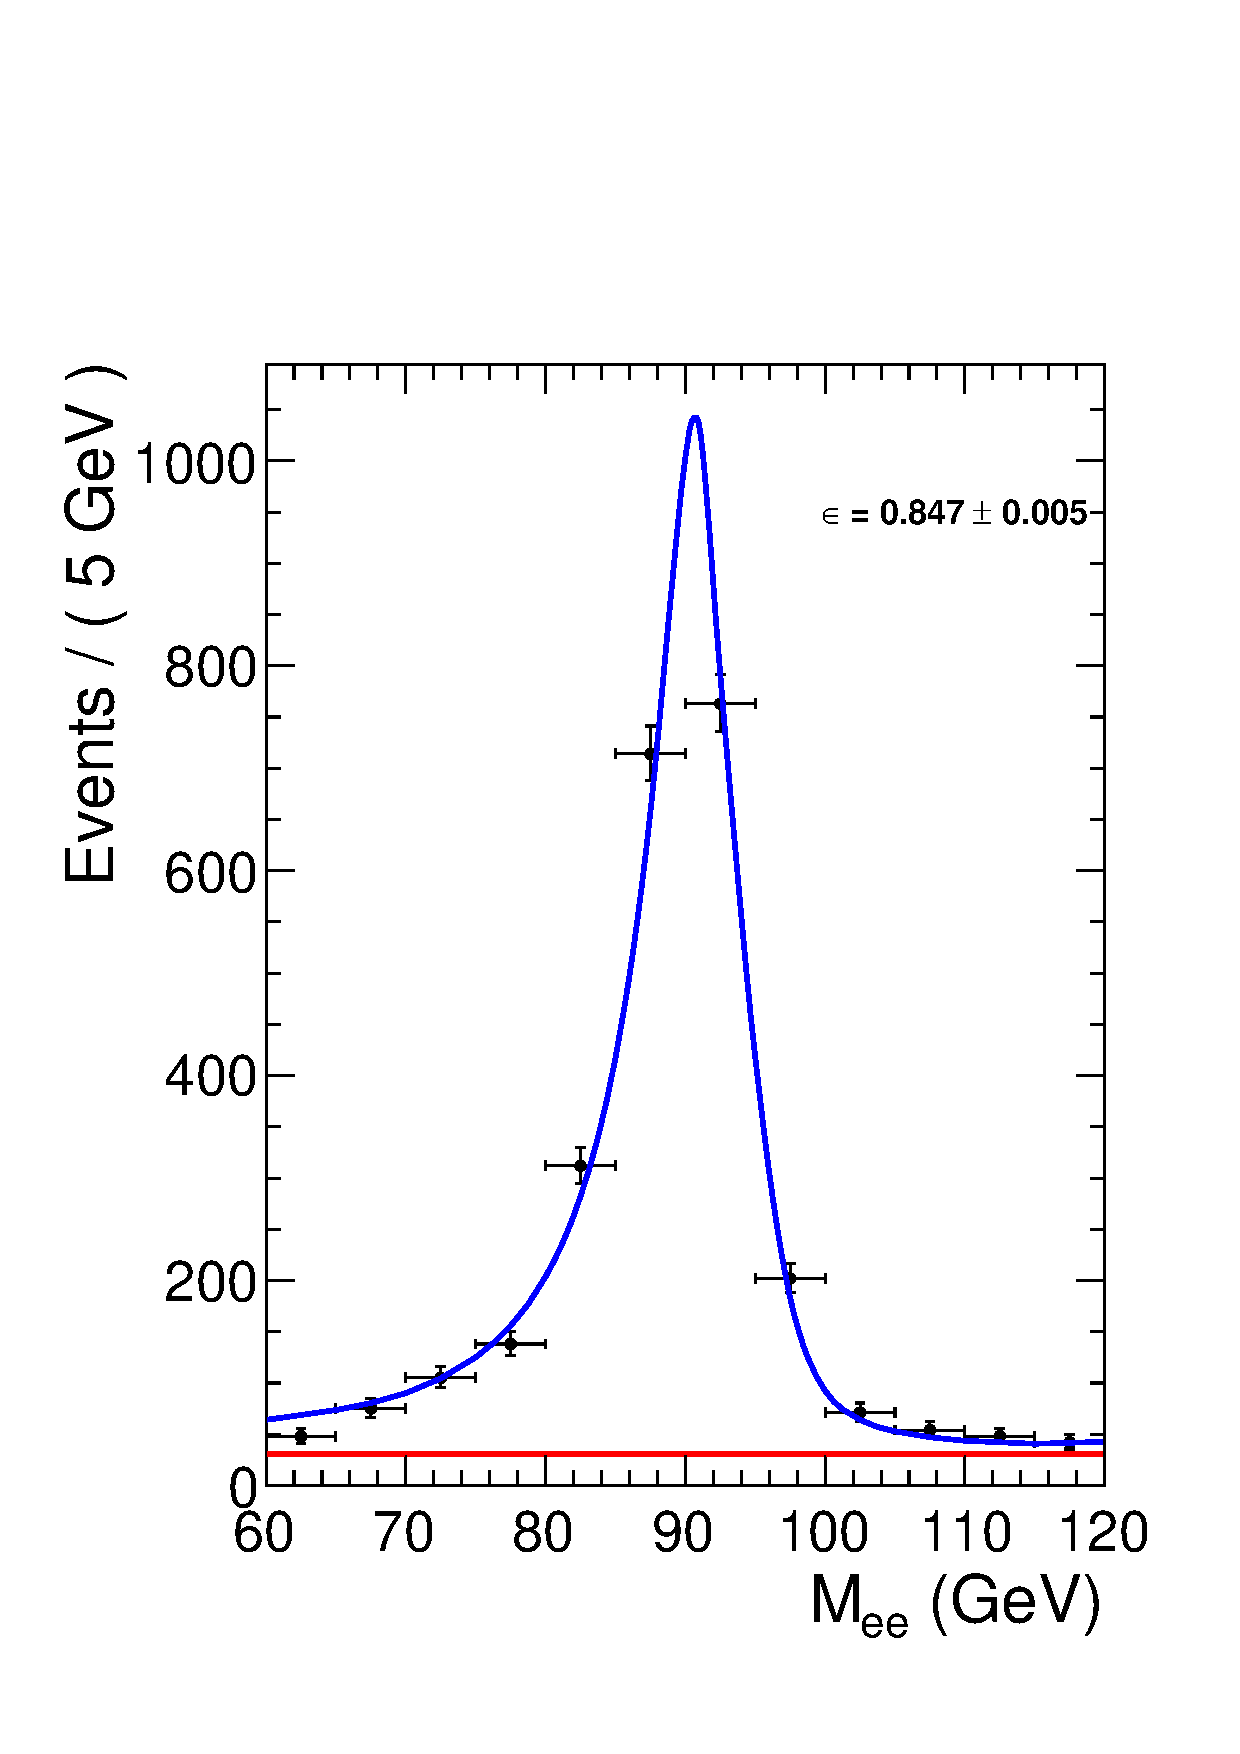
\includegraphics[width=1.0\textwidth]{figs/tpHistos_ID80_eb_fail.pdf}
%  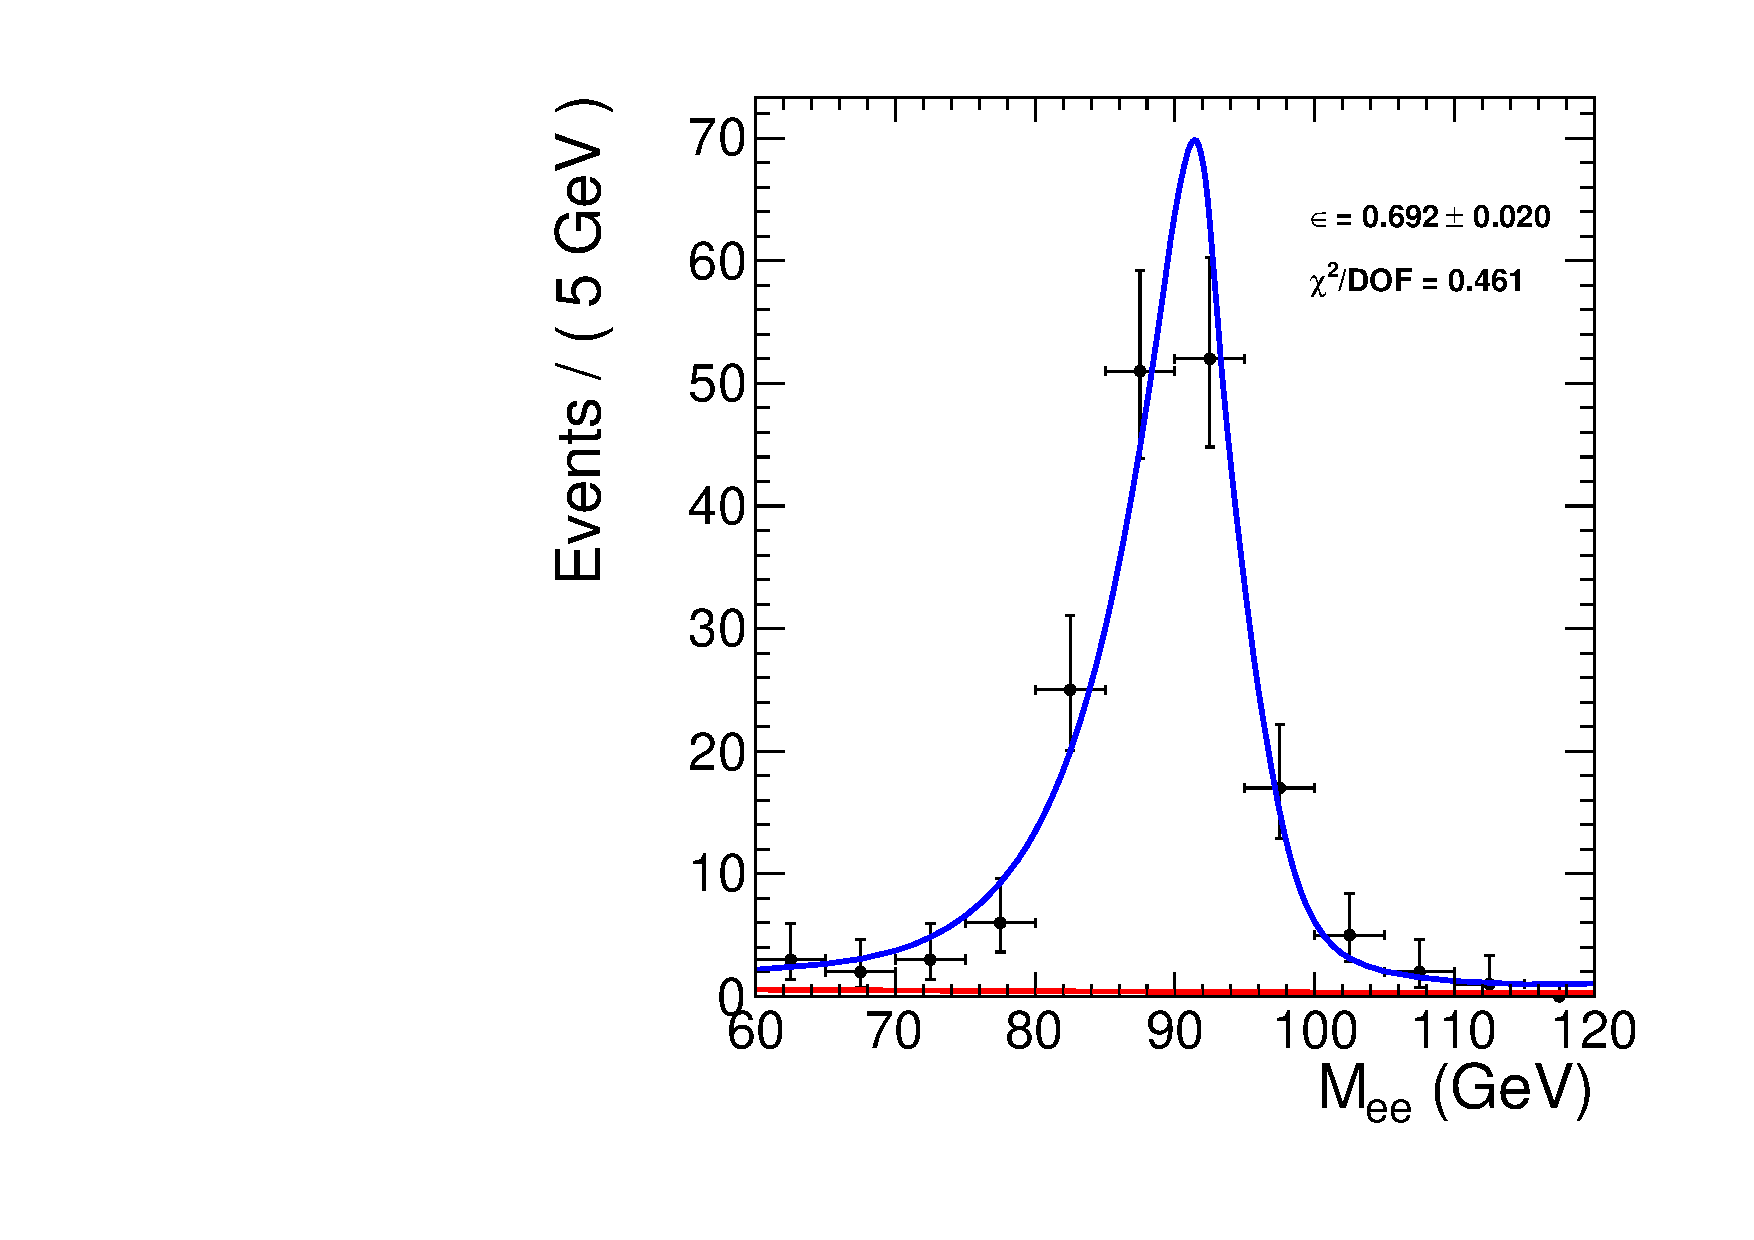
\includegraphics[width=1.0\textwidth]{figs/tpHistos_ID80_ee_fail.pdf}
% \end{minipage}
%% \begin{minipage}[W80toTrigger]{0.32\textwidth}
%%  \includegraphics[width=1.0\textwidth]{figs/TNPe_fake.png}
%%  \includegraphics[width=1.0\textwidth]{figs/TNPe_fake.png}
%% \end{minipage}
% \end{center}
%\caption{Extraction of \TNP efficiencies in the data from fits
%to the dielectron mass distributions for passing (upper row) and failing (lower row) probes:
%GSF-electron $\to$ tight selection for ECAL Barrel (left column) and ECAL Endcaps (right column). 
%The red line represents the background estimation.
%\label{fig:e-TNP}}
%\end{figure}
%Examples of \TNP fits on the data are given in Fig.~\ref{fig:e-TNP}
%for illustration.
%% can't cite an AN
%% All the details of the \TNP fits can be found in~\cite{CMS_AN_2010-323}.


%In addition to efficiencies, we report data/MC efficiency
%ratios $\rhoeff$, also called data/MC correction factors:
%\begin{equation}
%  \rho_{\textrm{eff-X}} = \frac{\EPS{TNP-X}(\textrm{data})}{\EPS{TNP-X}(\textrm{MC})}  \ \ \ 
%\textrm{and} \ \ \ \EPS{X} = \EPS{MC-X} \times \rho_{\textrm{eff-X}} ,
%\end{equation}
%where $\EPS{X}$ is the final electron efficiency
%and $\EPS{MC-X}$, the ``true''
%MC efficiency, for selection $X$ (reco, tight selection, HLT or overall).

The \TNP event selection efficiencies in the simulation 
are determined from large samples of signal events with no
background added.

%The main reason for considering data/MC correction factors rather
%than absolute efficiencies is that some biases cancel in the ratio.
%One bias that affects the $W$ analysis comes from the fact that,
%due limited statistics, we consider only two bins
%in pseudorapidity (EB and EE). In each bin efficiencies are weighted
%by the pseudorapidity distribution of electrons from Z decays,
%which is different from that of electrons from W$^+$ or W$^-$ decays.
%Hence, any $\eta$ dependence of the efficiency within the bin induces
%a bias, which is expected to cancel in the ratio (assuming that
%the dependence is roughly reproduced in the simulation).

The \TNP efficiencies are measured for the EB and EE electrons separately.
Tag-and-probe efficiencies are also determined separately by charge, 
to be used in the measurements of the W$^+$ and W$^-$ cross sections and their ratio.
%For this selection, only the charge of the probe is considered except for the
%determination of the reconstruction efficiency, where the probe (which is an
%ECAL cluster) is assigned the charge opposite to that of the tag.
%Tag-and-probe electron efficiencies, for the data and the Monte Carlo 
%simulation, and efficiency correction factors, are summarized in 
%Table~\ref{tab:e-eff-summary}. 
Inclusive efficiencies and correction factors are summarized in 
Table~\ref{tab:e-eff-summary}. The \TNP measurements of the efficiencies 
on the right-hand side of Eq.~(\ref{eq:e-eff})
are denoted as $\EPSTNPREC$, $\EPS{\tnp-tight}$, and $\EPSTNPTRG$.

%--------------------------------------------------
\begin{table}[htbp] %
\begin{center}
\caption[.]{\label{tab:e-eff-summary}
Tag-and-probe efficiencies in data and simulation, and the correction factors
used in the electron channels for the barrel (EB) and endcaps (EE). The combined statistical and systematic 
uncertainties are quoted. }
\begin{tabular}{|l|c|c|c|}
\hline
Efficiency & Data & Simulation & Data/simulation ($\rhoeff$) \\
\hline
\hline
\multicolumn{4}{|c|}{EB} \\
\hline
 \EPS{\tnp-rec}      & \WPWIEBEFFRECO  & \WPWIEBMCRECO & \WPWIEBRRECO \\
 \EPS{\tnp-tight}    & \WPWIEBEFFID    & \WPWIEBMCID   & \WPWIEBRID   \\
 \EPS{\tnp-trg}      & \WPWIEBEFFHLT   & \WPWIEBMCHLT  & \WPWIEBRHLT  \\
\hline
 \EPS{\tnp-all}  & \WPWIEBEFF  & \WPWIEBMC & \WPWIEBR \\
\hline
\hline
\multicolumn{4}{|c|}{EE} \\
\hline
 \EPS{\tnp-rec}       & \WPWIEEEFFRECO  & \WPWIEEMCRECO & \WPWIEERRECO \\
 \EPS{\tnp-tight}    & \WPWIEEEFFID    & \WPWIEEMCID   & \WPWIEERID   \\
 \EPS{\tnp-trg} & \WPWIEEEFFHLT   & \WPWIEEMCHLT  & \WPWIEERHLT  \\
\hline
 \EPS{\tnp-all}  & \WPWIEEEFF  & \WPWIEEMC & \WPWIEER \\
\hline
\end{tabular}
\end{center}
\end{table}


\par
Event selection efficiencies are measured with respect to the W events
within the ECAL acceptance.
Simulation efficiencies estimated from {\sc POWHEG} $\Wo$ samples 
are shown in Table~\ref{tab:el-Weff}.
These are efficiencies at the event level,
e.g.: they include efficiency loss due to the second electron veto.  
Given the acceptances listed in Table~\ref{tab:WZlaccgen} and the \TNP 
efficiencies listed in Table~\ref{tab:e-eff-summary},
the overall efficiency correction factors for electrons from $\Wo$ decays are computed.
The overall $\Wo$ signal efficiencies, obtained as products of simulation efficiencies
with data/simulation correction factors, are listed in Table~\ref{tab:el-Weff}.
%These efficiencies are relative to $\Wo$ events with the electron within the acceptance,
%as described above. 
%Theoretical uncertainties on the efficiencies related to the PDF uncertainties and 
%the PDF choice are negligible.
\begin{table}[ht] %
  \begin{center}
  \caption{ Simulation efficiencies and the final corrected selection efficiencies for the 
$\Wp$, $\Wm$, and their average, in the $\Wen$ analysis. The quoted uncertainties are 
statistical for $\effmc$ and include both statistical and systematic uncertainties 
for the corrected efficiencies $\effmc \times \rhoeff$.
  \label{tab:el-Weff}}
  \begin{tabular}{|l|c|c|}
    \hline
     & $\effmc$  &  $\effmc \times \rhoeff$ \\
    \hline\hline
 $\Wpen$   & \WEPEFFMC  & \WEPEFF \\
 $\Wmen$   & \WEMEFFMC  & \WEMEFF \\
 $\Wen$  & \WEIEFFMC  & \WEIEFF \\
    \hline
    \end{tabular}
  \end{center}
\end{table}

The efficiencies and the data/simulation ratios are also estimated in bins of the electron 
$\Et$ and $\eta$ in order to examine in detail the detector performance and take into 
account the differences in the W and Z kinematic distributions. 
The data/simulation ratios for reconstruction, selection, and trigger are shown 
in Fig.~\ref{fig:e-TnPratios} as functions of the electron $\Et$ and $\eta$.

The reconstruction data/simulation ratios appear to be uniform with respect to $\Et$ and $\eta$, so
a smaller number of bins is sufficient for the determination of their values.
%Based on this fact our choice was to quote as reconstruction 
%efficiency the estimation in two $\eta$ bins only (in ECAL Barrel and ECAL Endcaps).
The data/simulation ratios for the selection and trigger efficiencies show a dependence 
that is estimated using ten $\eta$ bins and six $\Et$ bins. Data/simulation ratios are estimated for 
both electron charges as well. 

The binned ratios and simulation efficiencies are transferred into the W analysis by properly weighting 
their product in each ($\Et$, $\eta$) bin by the relative ECAL cluster abundance
estimated from {\sc POWHEG} simulations. The corrected efficiencies are compared with the 
two-bin case in which the efficiencies are estimated in two bins of $\eta$ (EB and EE). 
The multibin corrected efficiencies are found to be consistent with the  two-bin 
corrected efficiencies within the assigned uncertainties. 
% In order to be sure that no hidden systematic uncertainty is missed,  half of the 
% maximum difference between the multibin and two-bin corrected efficiencies 
% is propagated as an additional systematic uncertainty on the two-bin efficiencies used to estimate the cross 
% sections. The additional relative uncertainty is at the level of 0.6$\%$.  


\begin{figure}[htbp]
\begin{center}
% \begin{minipage}[Reconstruction]{0.64\textwidth}
  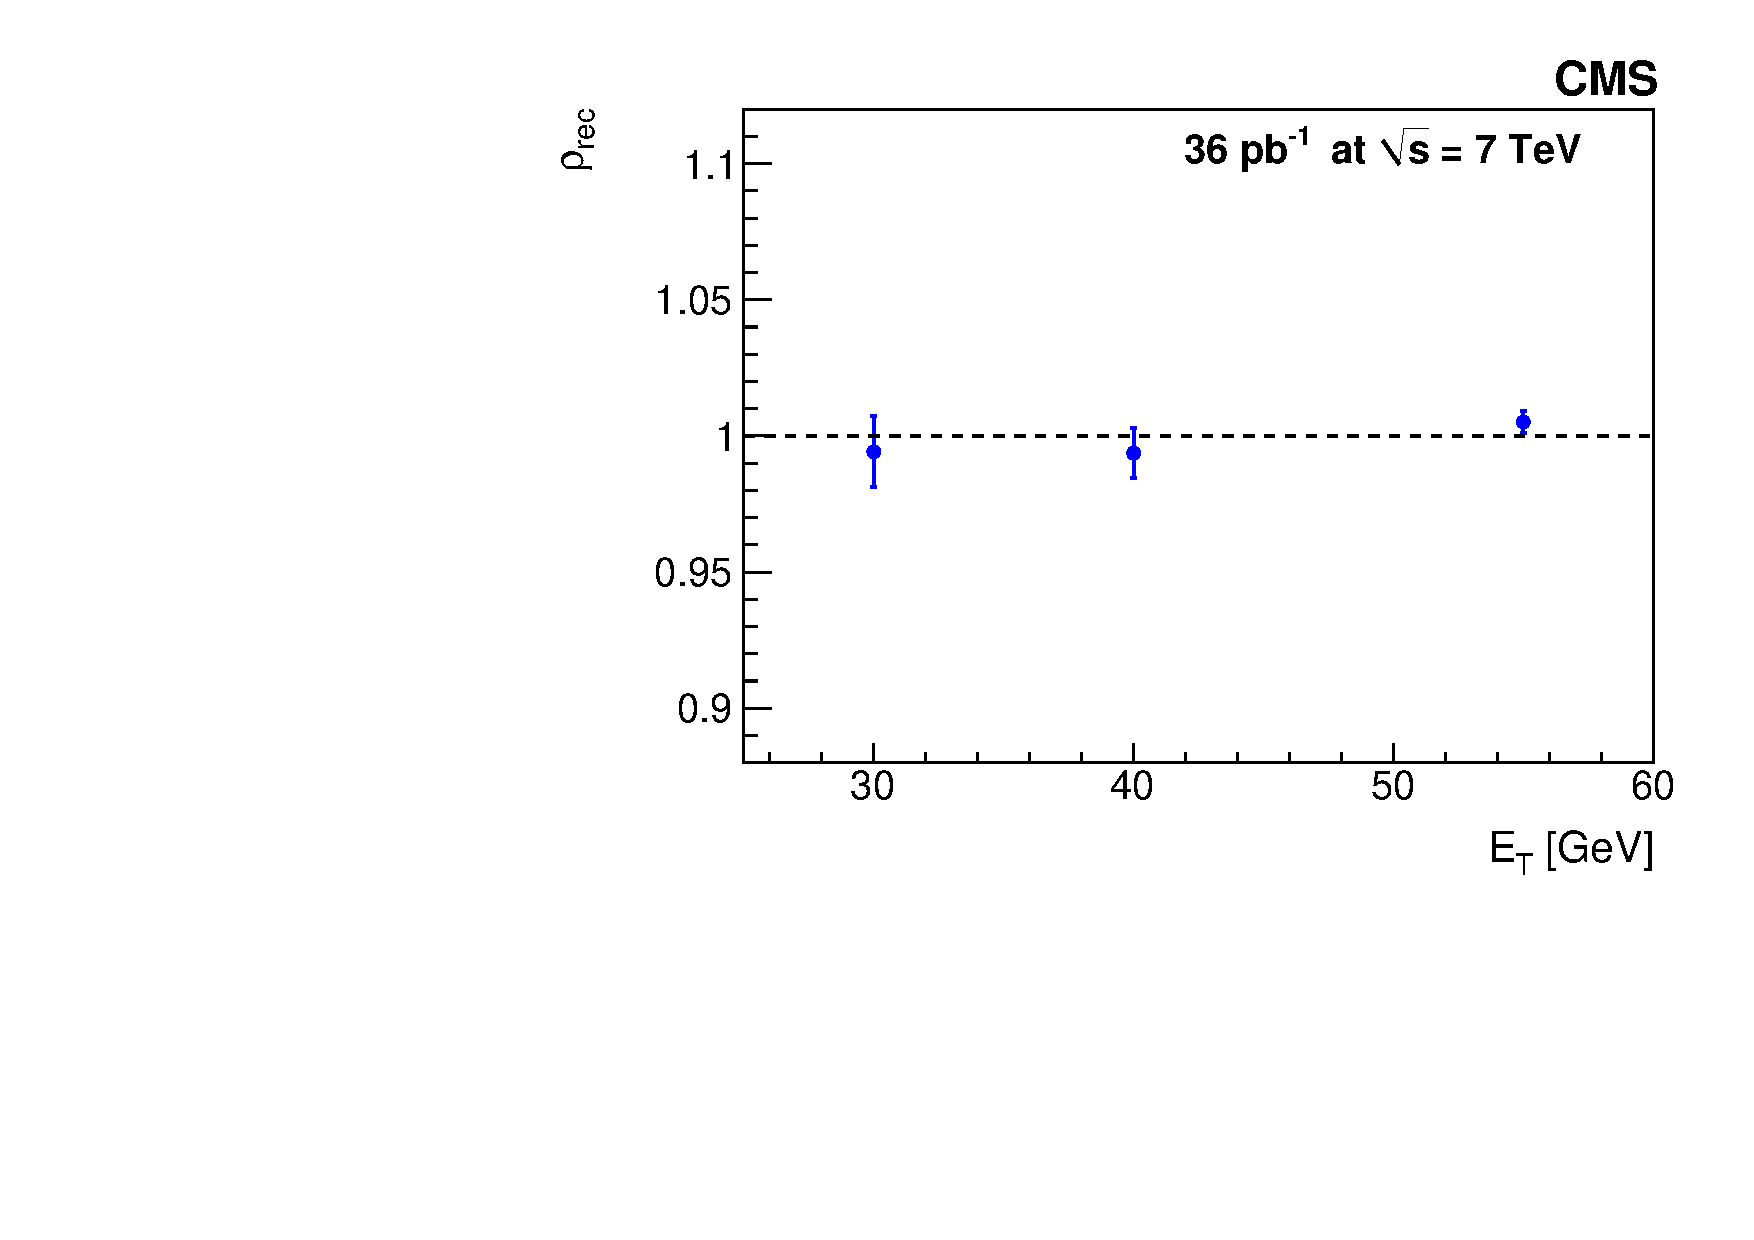
\includegraphics[width=0.48\textwidth]{figs/recoeff_scalept.pdf}
  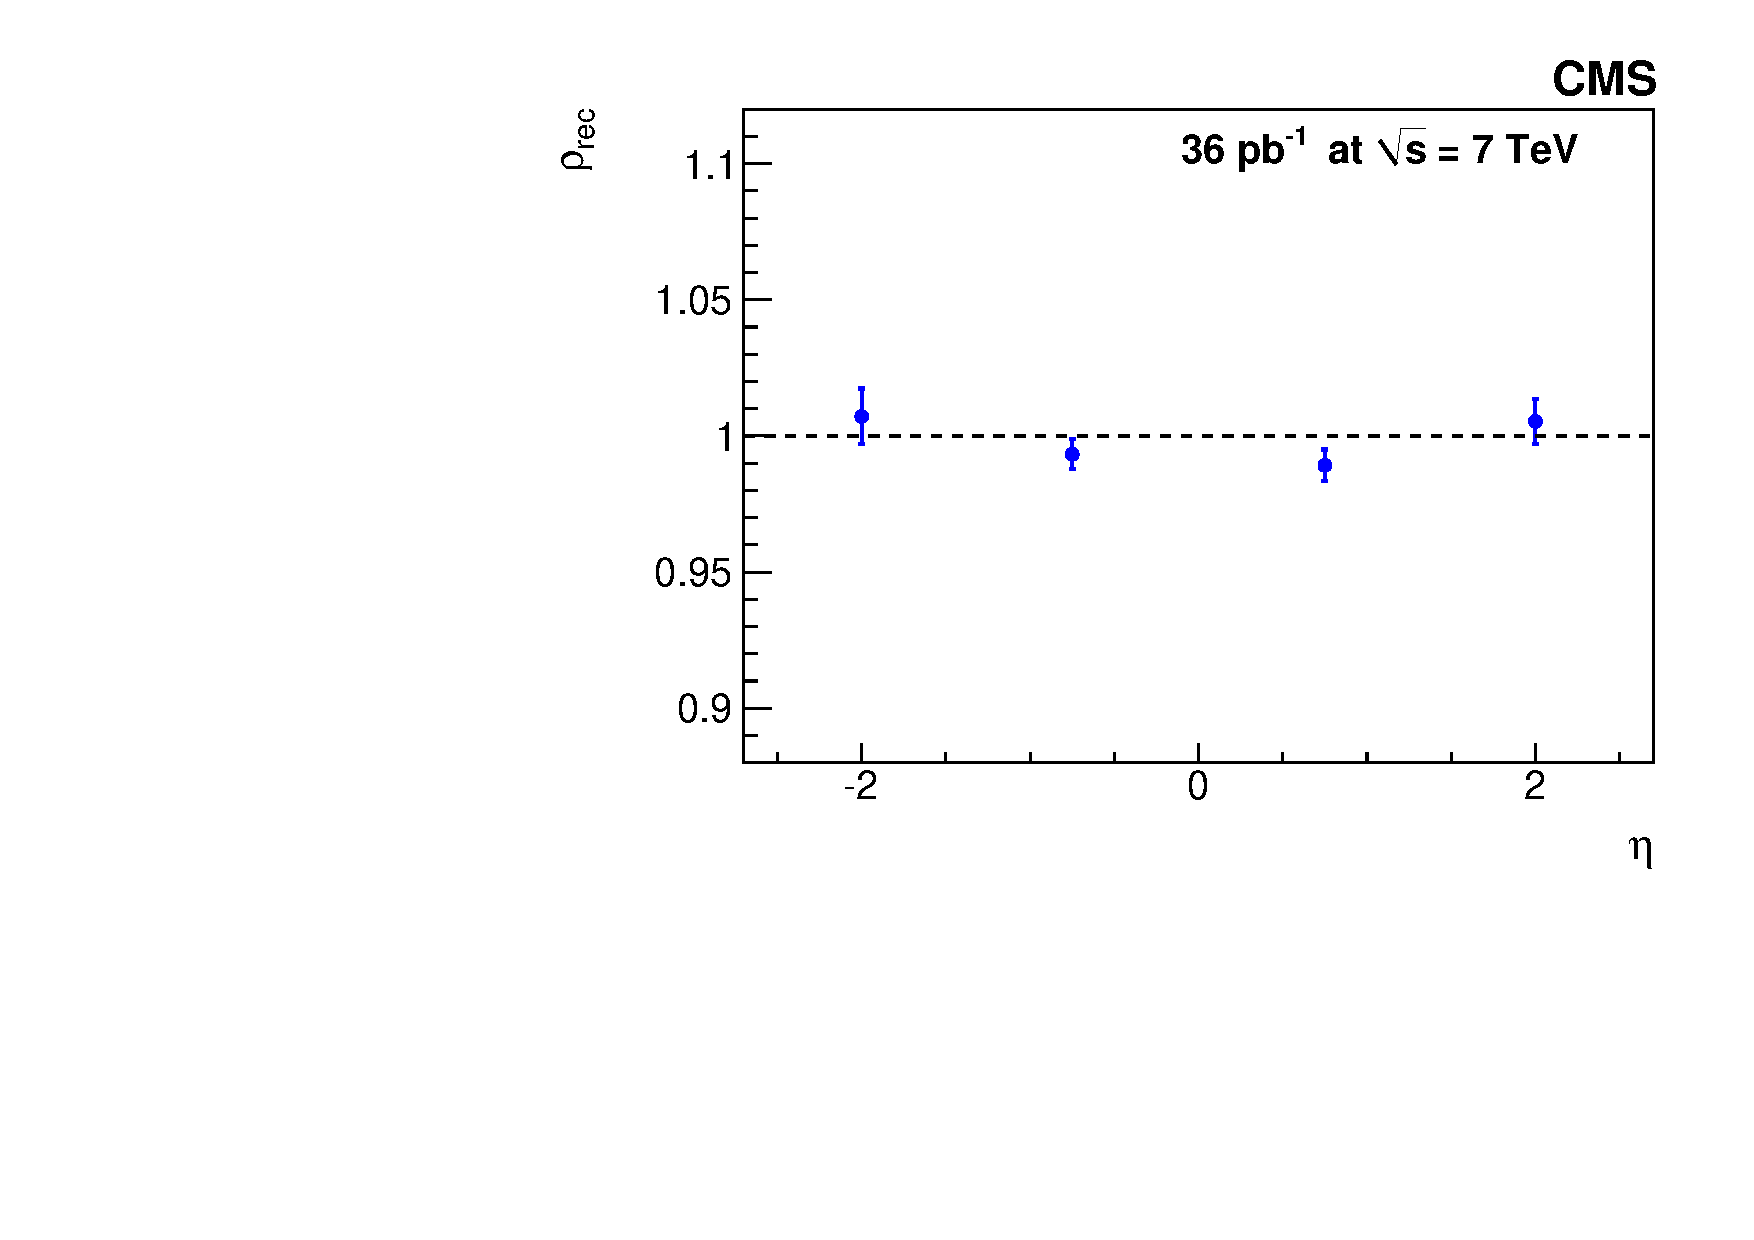
\includegraphics[width=0.48\textwidth]{figs/recoeff_scaleeta.pdf}
% \end{minipage}
% \begin{minipage}[WP80]{0.64\textwidth}
  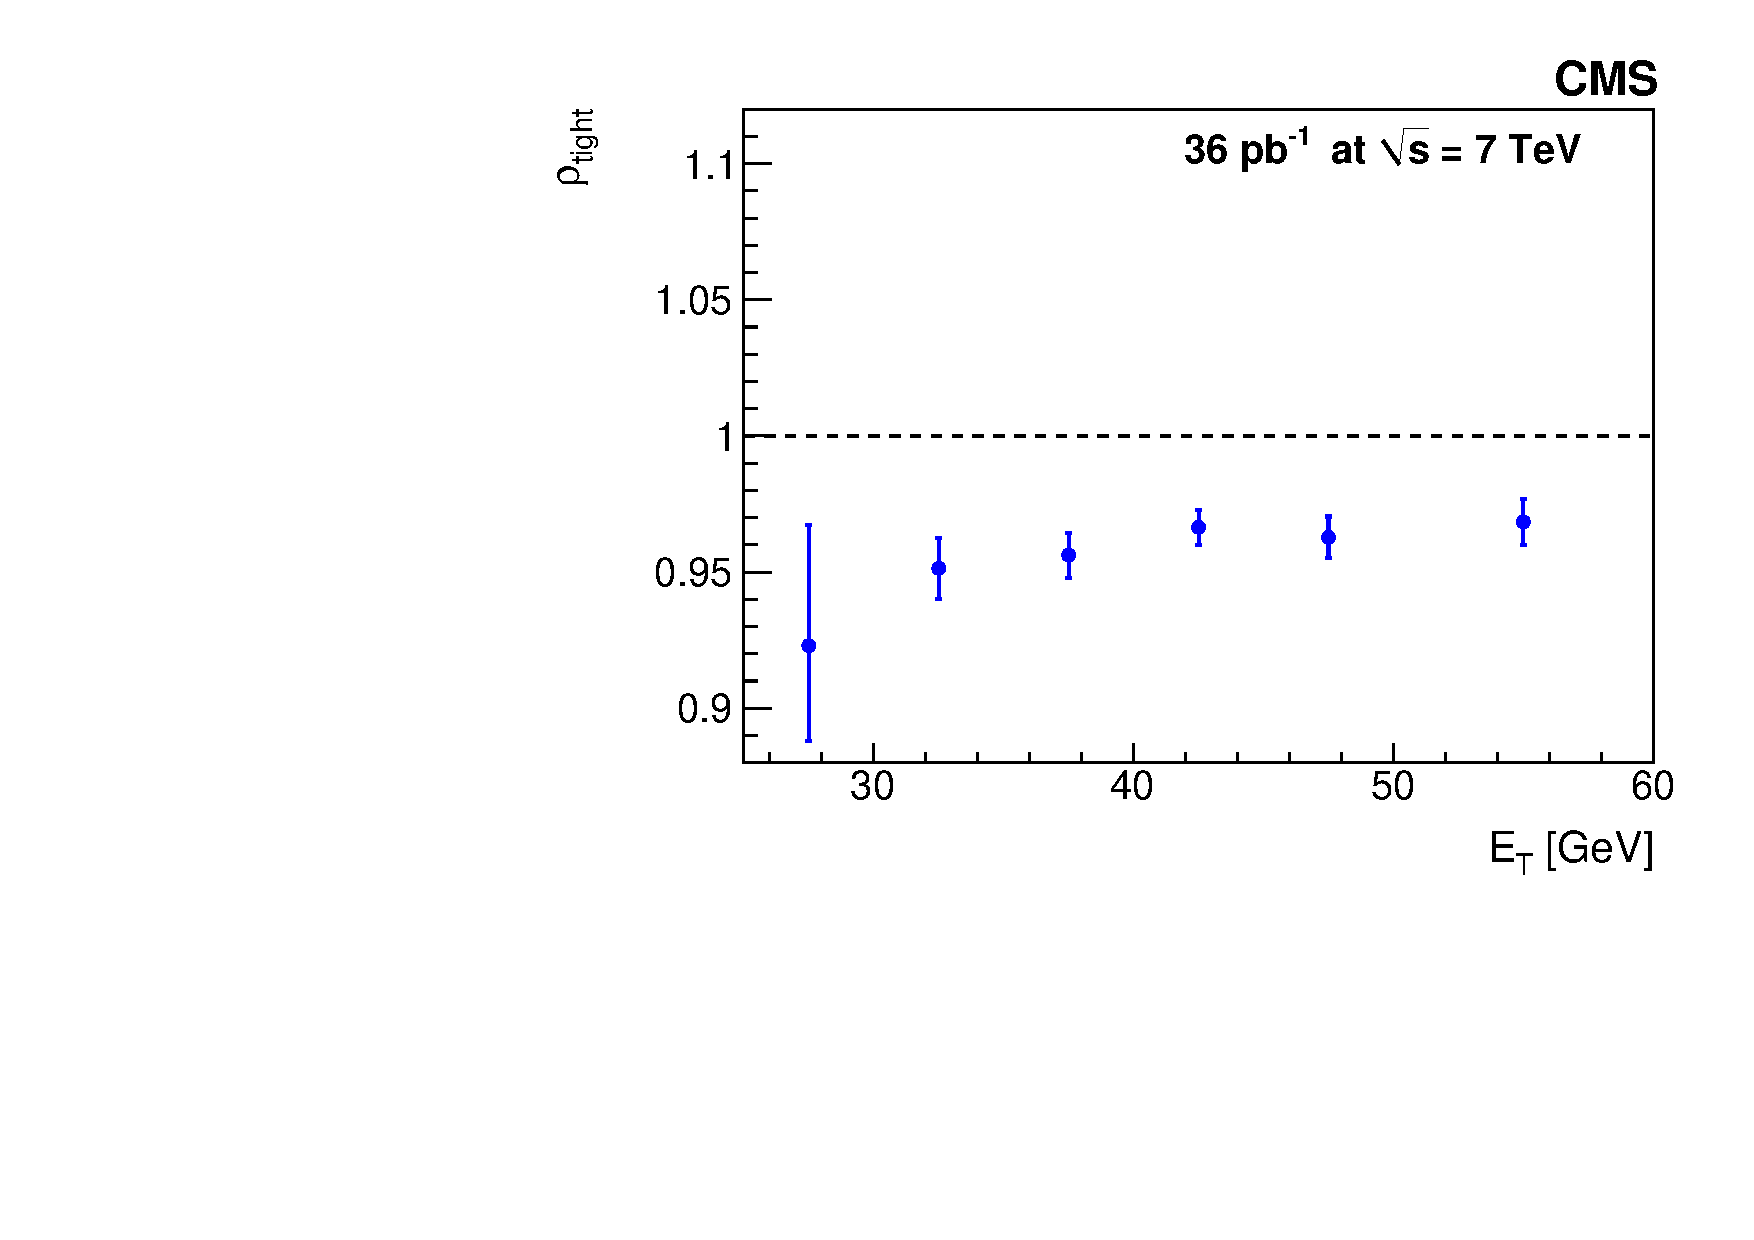
\includegraphics[width=0.48\textwidth]{figs/eleideff_scalept.pdf}
  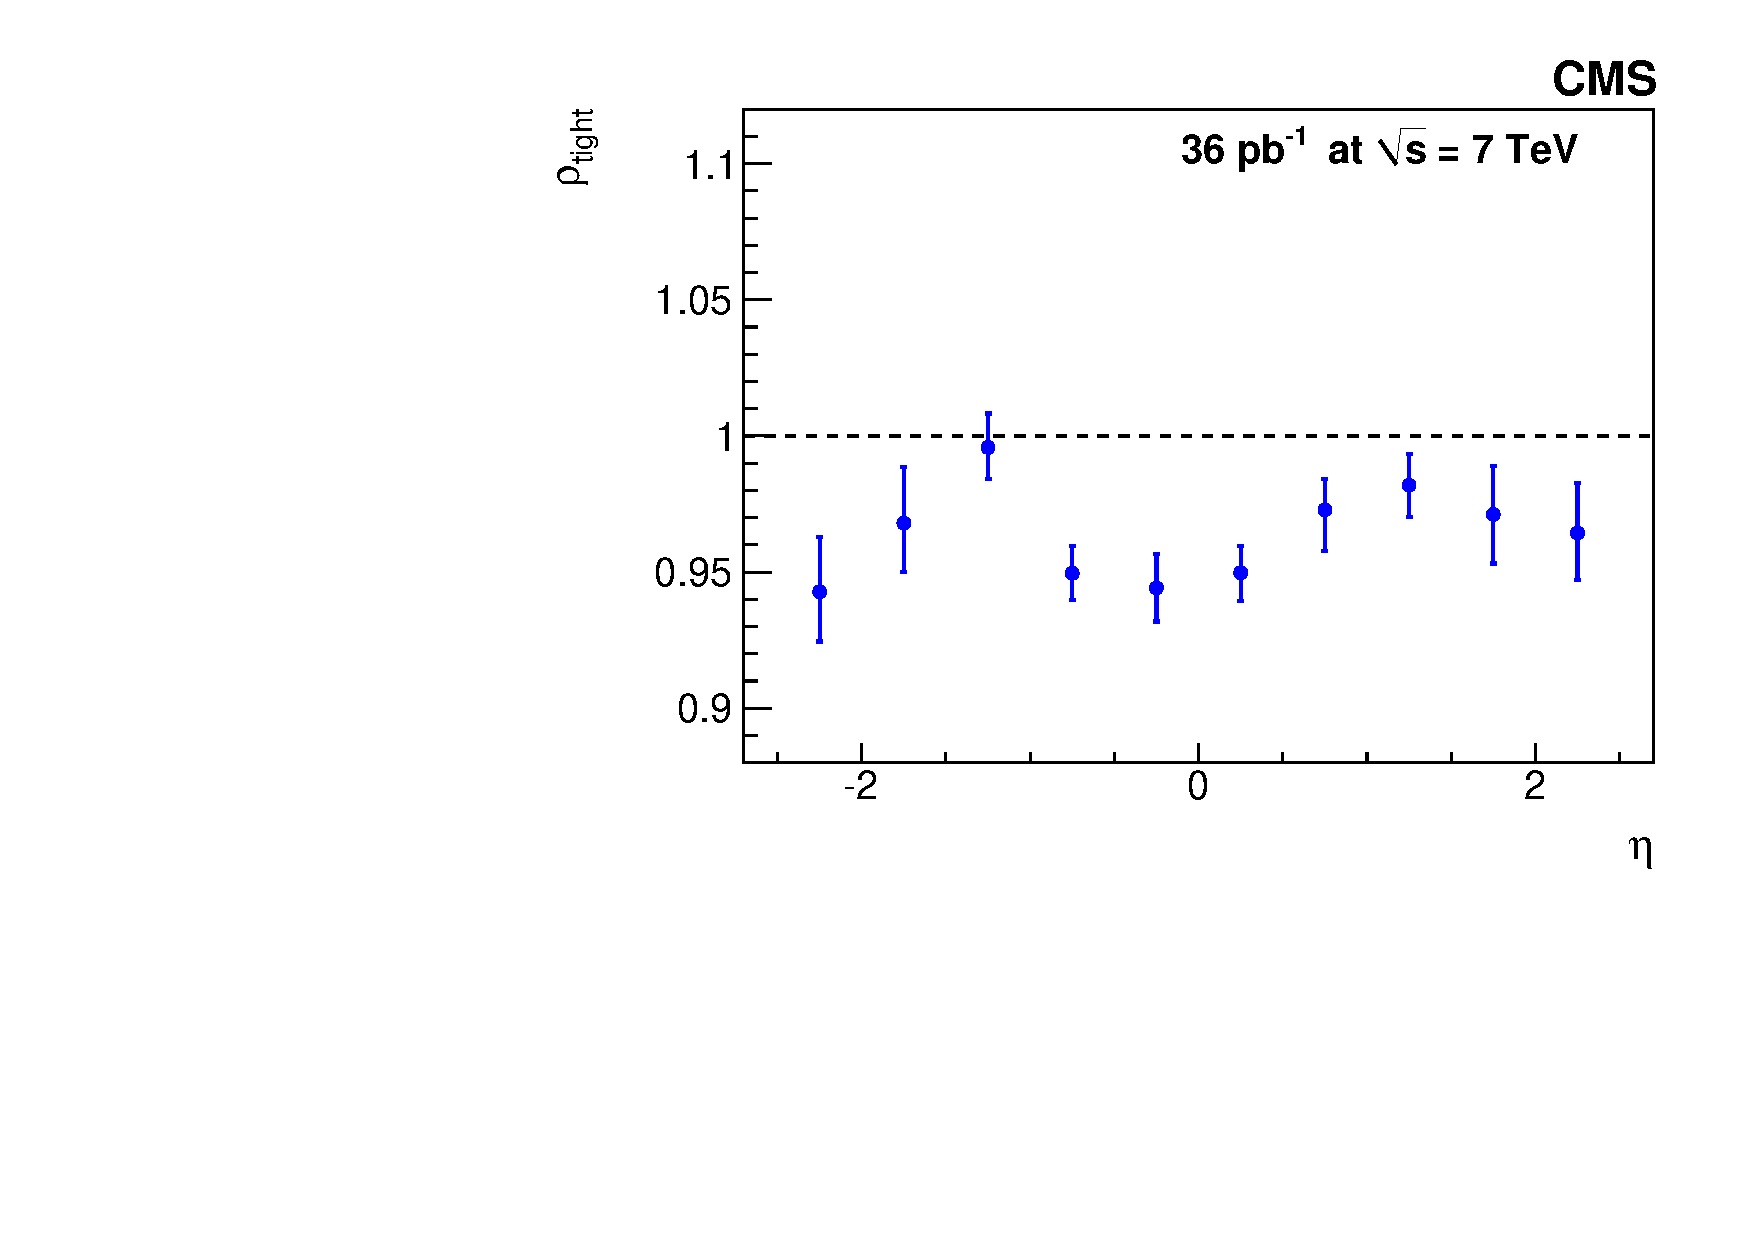
\includegraphics[width=0.48\textwidth]{figs/eleideff_scaleeta.pdf}
% \end{minipage}
% \begin{minipage}[W80toTrigger]{0.64\textwidth}
  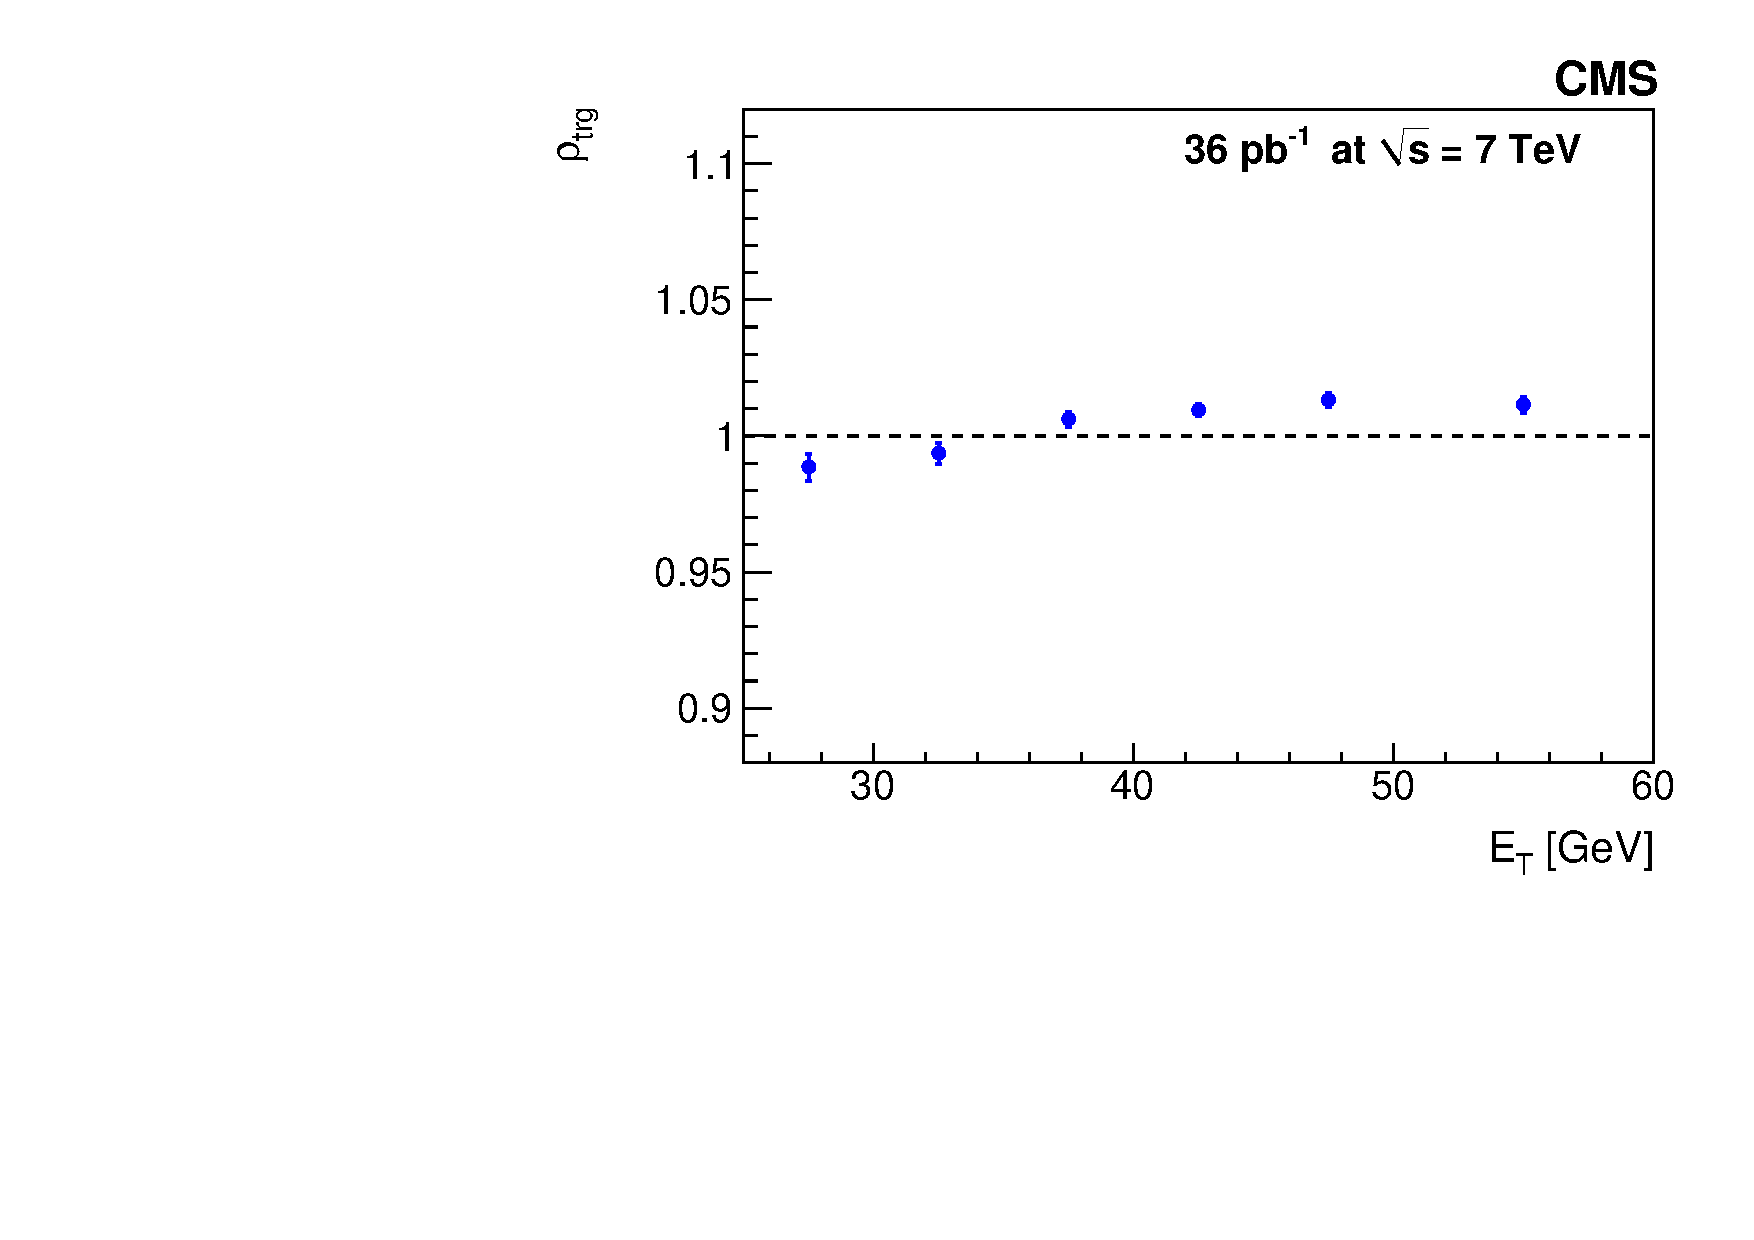
\includegraphics[width=0.48\textwidth]{figs/trigeff_scalept.pdf}
  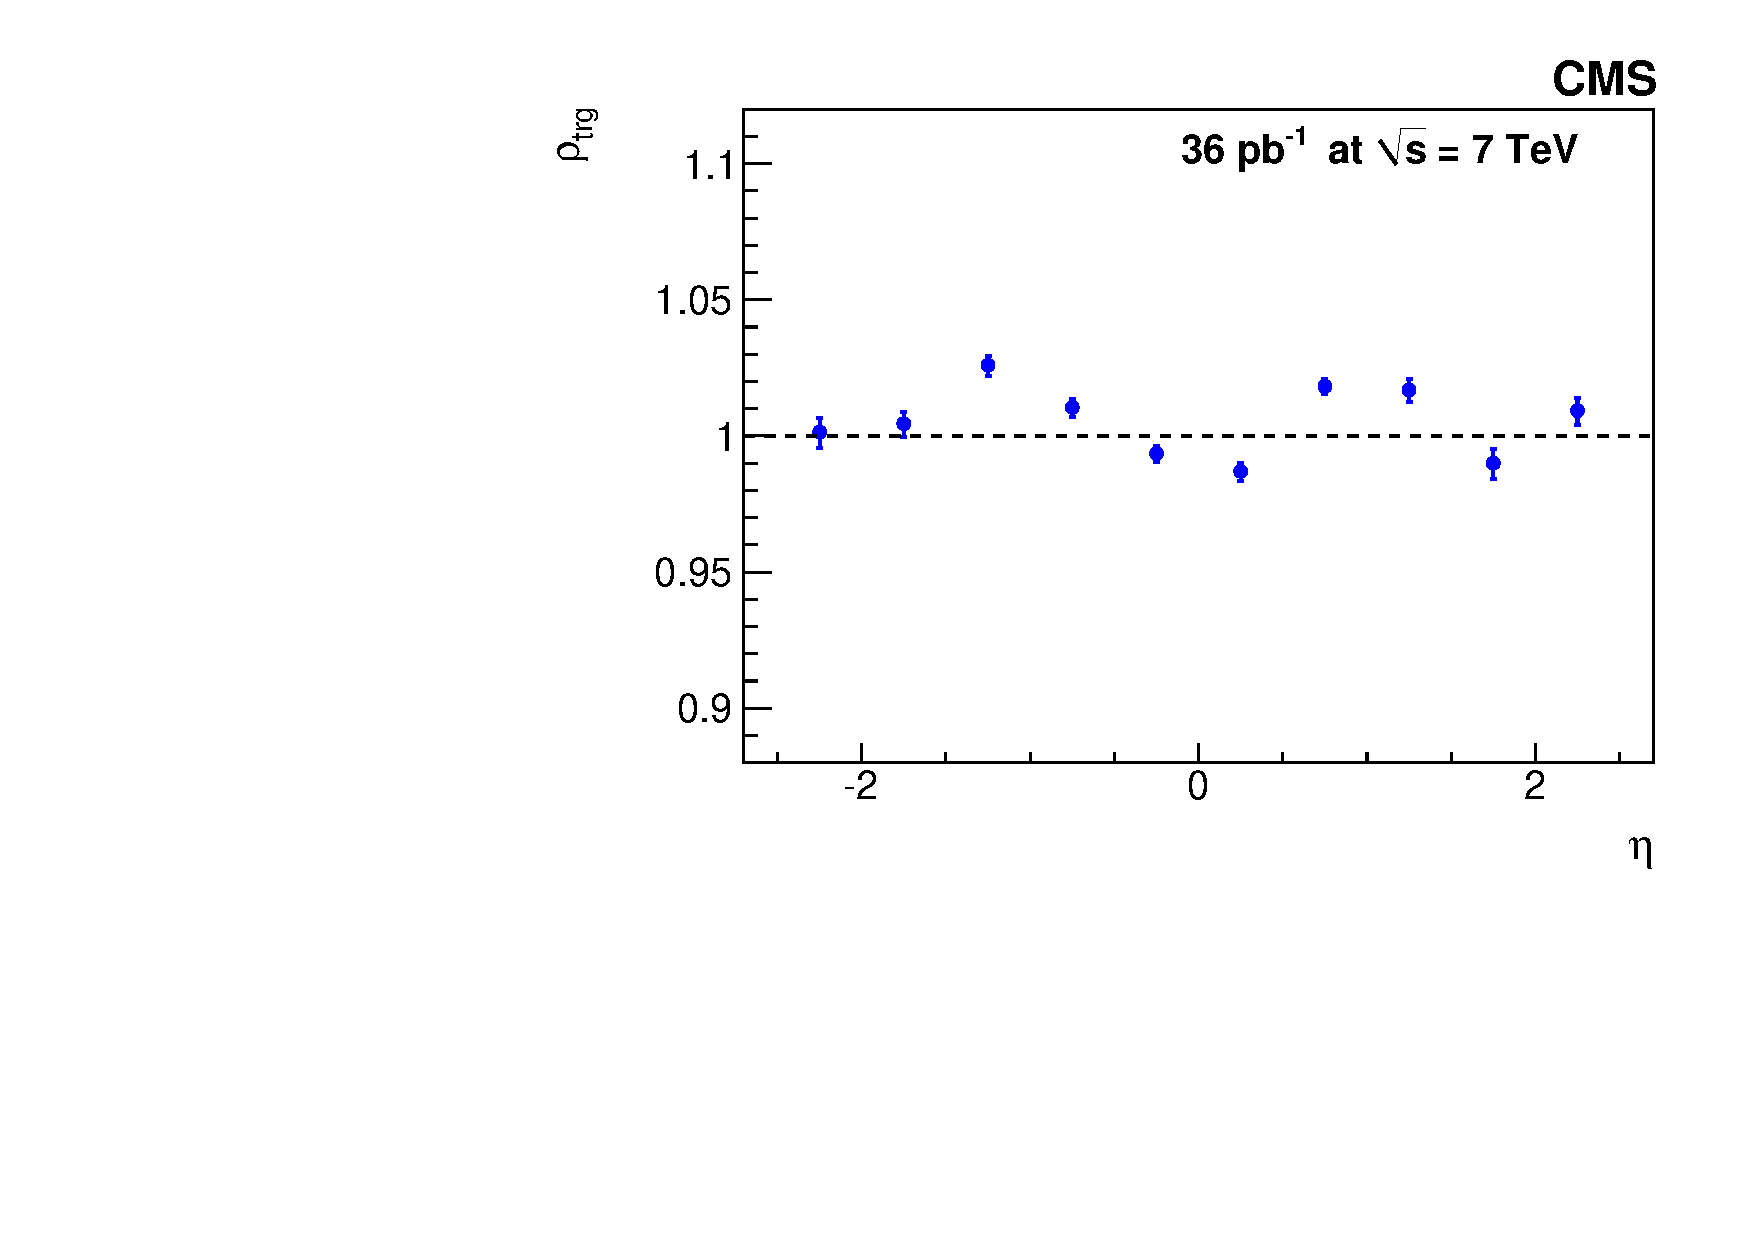
\includegraphics[width=0.48\textwidth]{figs/trigeff_scaleeta.pdf}
% \end{minipage}
 \end{center}
\caption{Data/simulation \TNP ratios versus electron $\Et$ (left column) and $\eta$ (right column).
The ratios are presented for the reconstruction ($\rho_\mathrm{rec}$, top row), selection 
($\rho_\mathrm{tight}$, middle row), and trigger ($\rho_\mathrm{trg}$, bottom row) efficiencies.
Points with error bars represent the ratio measured in data; dashed lines correspond to a constant ratio of one.
\label{fig:e-TnPratios}}
\end{figure}


The $\Zo$ selection efficiencies for data and simulation are obtained based
on the \TNP efficiencies
listed in Table~\ref{tab:e-eff-summary}  and
the event acceptances given in Table~\ref{tab:WZlaccgen}.
The $\Zo$ efficiencies are first determined after
reconstruction and identification (as products of
single-electron efficiencies).
The event trigger efficiency is computed
as the probability that at least one of the two electrons
satisfies the L1+HLT requirement. 
The overall selection efficiency for the $\Zo$ analysis is
the product of the reconstruction, identification, and trigger 
efficiencies. The simulation efficiency obtained from the {\sc POWHEG} $\Zo$ 
samples, together with the final corrected $\Zo$ selection efficiency 
$\effmc \times \rhoeff$, are shown in Table~\ref{tab:el-Zeff}.
These efficiencies are relative to the $\Zo$ events with both electrons within the ECAL acceptance.
%Similarly to the W case, the PDF uncertainties on the corrected $\Zo$ efficiencies 
%were found to be negligible.
\begin{table}[ht] %
  \begin{center}
  \caption{ Simulation efficiency and the final corrected selection efficiency for the ~$\Zee$ analysis.
The quoted uncertainties are statistical for $\effmc$ and include both statistical and 
systematic uncertainties for the corrected efficiency $\effmc \times \rhoeff$.
 \label{tab:el-Zeff}}
  \begin{tabular}{|l|c|c|}
    \hline
     & $\effmc$ & $\effmc \times \rhoeff$ \\
    \hline\hline
    $\Zee$  & \ZEEEFFMC & \ZEEEFF \\
    \hline
    \end{tabular}
  \end{center}
\end{table}


\par
%For later convenience, we define the quantity $A^{\prime}$, which is 
%the overall selection efficiency in the Monte Carlo simulation, as:
%\begin{equation}
%  A^{\prime} = A \times \epsilon
%            = A^{\textrm{ECAL}} \times \EPS{MC} \ .
%\end{equation}




%\subsection{Muon Efficiencies \label{sec:muonEff}}

The muon reconstruction overall selection efficiency 
is determined by the efficiency to find a track in the inner tracker and in the
muon chambers, to pass the isolation requirements, and the probability 
to pass the L1 trigger and HLT.

Tag-and-Probe method is used to determine muon efficiencies for $\Wmn$ cross section determination,
while for $\Zmm$ muon efficiencies are determined simultaneously with the Z yield using a simultaneous
fit technique that is described in Section~\ref{sec:Zmumu}. 
%Tag-and-Probe method uses a clean sample of $\Zmm$ candidates selected from the 36~pb$^{-1}$ available data
%on which about 22000 triggered muon {\em tags} are selected.
%$\Zmm$ events have muon kinematics very similar to those used in the $\Wo$ analysis.
%The possible presence of background processes in the selected event sample has been also taken into account.

%, making use of the 2 million events
%The efficiency ratio 
%$\rho_\mu = {\epsilon_{\mathrm{data}}}/{\epsilon_{\mathrm{MC}}}$ 
%has been calculated in order to be applied to the  
%W cross-section determination. 
The efficiencies have been studied as a function of muon pseudorapidity and transverse momentum, 
to reproduce better the real detector performance. 
The promediated efficiencies are estimated to be
$\epsilon_{\mathrm{data}} = 0.8548 \pm 0.0025\, \mathrm{(stat)} \pm  0.024\, \mathrm{(syst)}$ and
$\epsilon_{\mathrm{MC}} = 0.8989  \pm   0.0004\, \mathrm{(stat)}$ in data and Monte Carlo respectively,
hence a correction factor of $\rho_\mu= 0.9509 \pm  0.0028 \mathrm{(stat)} \pm  0.024\, \mathrm{(syst)}$
has been appled to the data.
The quoted systematic errors take into account the fit parameter uncertainties stemming 
from the correction of the background.

Single-muon efficiencies have also been determined separating in positive or negative charged muons, 
obtaining the following correction factors: $\rho_\mu^+ = 0.957 \pm 0.004\,\mathrm{(stat)} \pm 0.024\,\mathrm{(syst)}$,
$\rho_\mu^- = 0.945 \pm 0.004\,\mathrm{(stat)} \pm 0.024\,\mathrm{(syst)}$.

A small fraction (0.5\%) of muon events is lost because of Level-1 trigger pre-firing
due to the wrong assignment to the muon bunch crossing number, due to imperfect timing. 
Cross sections in muon channels have been corrected by this effect and
the uncertainty on the correction factor has been taken as systematic uncertainty.



\section{\texorpdfstring{The $\Wln$  Signal Extraction}{The W-> l nu  Signal Extraction}}
\label{sec:WsignalExtraction}

The signal and background yields are obtained by fitting
the $\MET$ distributions for $\Wen$ and $\Wmn$ to different
functional models.
An accurate $\MET$ measurement is essential for distinguishing
a $\PW$ signal from QCD multijet backgrounds.
We profit from the application of the PF
algorithm, which provides superior $\MET$
reconstruction performance~\cite{PFMET1} with respect to alternative
algorithms at the energy scale of the $\PW$ boson.
% The energy of photons is directly obtained from the ECAL measurement,
% corrected for zero-suppression effects.
% The energy of electrons is determined from a combination of the track
% momentum at
% the main interaction vertex, the corresponding ECAL cluster energy,
% and the energy sum of
% all bremsstrahlung photons attached to the track. The energy of muons
% is obtained from the
% corresponding track momentum. The energy of charged hadrons is
% determined from a combination
% of the track momentum and the corresponding ECAL and HCAL energy,
% corrected for
% zero-suppression effects, and calibrated for the non-linear response
% of the calorimeters. Finally
% the energy of neutral hadrons is obtained from the corresponding
% calibrated ECAL and HCAL
% energy.


The $\MET$ is the magnitude of the transverse component of the missing momentum
vector, computed as the negative of the vector sum of all
reconstructed transverse momenta of particles identified with
the PF algorithm. The algorithm combines the information from
the inner tracker, the muon chambers, and the calorimeters
to classify reconstructed objects according to particle type
(electron, muon, photon, or charged or neutral hadron),
thereby allowing precise energy corrections.
The use of the tracker information reduces the sensitivity of $\MET$ to miscalibration of the calorimetry.
%also providing a significant degree of redundancy that
%reduces the sensitivity of the $\MET$ measurements
%to miscalibrations of the calorimetry.
%\par
%The impact of anomalous noise signal in the calorimeters is reduced to
%a negligible level~\cite{metPAS}.

\par
The QCD multijet background is one of the most significant backgrounds in W analyses.
At high $\MET$, EWK backgrounds, in particular $\Wtn$ and DY,
also become relevant, leading to contamination levels on the
order of $10\%$.

The $\MET$ model is fitted to the observed distribution as the sum of three contributions:
the W signal, and the QCD and EWK backgrounds.
The EWK contributions are normalized to the W signal yield in the fit
through the ratios of the theoretical cross sections.

Simultaneous fits are performed to the two $\MET$ spectra of W$^+$ and W$^-$ candidates,
fitting either the total W cross section and
the ratio of positive and negative W cross sections, or
the individual positive and negative W cross sections.
In both cases the overall normalization of QCD multijet events is determined from the fit.
The diboson and $\ttbar$ contributions,
taken from simulations, are negligible (Section~\ref{sec:EWKbkgds}).


\par
In the following sections the modeling
of the $\MET$ shape for the signal and the EWK backgrounds are presented,
and the methods used to determine
the $\MET$ shape for the QCD multijet background from data are
 described.
Finally, the extraction of the signal yields is discussed.



%\section{Missing Transverse Energy\label{sec:MET}}
An accurate $\MET$ measurement is essential for distinguishing
$\Wo$ signal from QCD backgrounds. We use $\MET$ estimate provided
by the Particle Flow (PF) algorithm which showed the best performance for the
CMS detector. Details on Particle Flow $\MET$ are provided in Ref.~\cite{PFMET}. 
\par
We have very good agreement of the $\MET$
distributions in $\Wln$ in data and simulation~\cite{metPAS}.
\par
The $\MET$ is computed as the vector sum of all PF objects.
The resolution for inclusive multi-jet samples and for
$\Wln$ events is well reproduced by the 
simulation.  A modest broadening of about $10\%$ is observed 
when there is more than one primary vertex; this occurs in less 
than $40\%$ of the events and has a negligible impact on the
extraction of the $W$ yields described below.



\subsection{\texorpdfstring{Signal ${E\!\!/}_{\!\mathrm{T}}$  Modeling}{Signal ET Modeling}}
\label{sec:WsignalMETtemplate}

The $\Wln$ signal is extracted with methods that employ
simulation predictions of the $\MET$ distribution in signal events.
These predictions
rely on the modeling of the vector-boson recoil and detector effects that
can be difficult to simulate accurately. Discrepancies could result
from deficiencies in the modeling of the
calorimeter response and resolution, and from an incomplete description of
the underlying event.
% and from simplifications made in the simulation of pile-up.
These residual effects are addressed using corrections
determined from the study of Z-boson recoil in data, discussed in the following paragraph.

The recoil to the vector boson is defined as the negative of the vector
sum of transverse energy vectors of all particles reconstructed with the PF algorithm
in W and Z events, after subtracting the contribution from the daughter lepton(s).
The recoil is determined for each event in $\Zll$ data and simulated $\Zll$
and $\Wln$ samples.
We fit the distributions of the recoil components (parallel and perpendicular to the
boson p$_T$ direction) with a double Gaussian, whose mean and width vary with the boson
transverse momentum.
For each sample, we fit polynomials to the extracted mean and width of the recoil
distributions as functions of the boson transverse momentum.
The ratios of data to simulation fit-parameters from the $\Zo$ samples are used as scale
factors to correct the polynomials parameters of the W simulated recoil curves.
For each $\Wo$ simulated event, the recoil is replaced with a value drawn from the
distribution obtained with the corrected parameters corresponding to the $\Wo$ p$_T$.
The $\MET$ value is calculated by adding back the energy of the $\Wo$ lepton.
%We fit the recoil distributions whose mean and width vary with the boson transverse
%momentum. For each sample, we fit polynomials to the extracted means and widths of the recoil
%distributions as functions of the boson transverse momentum.
%The ratios of data to simulation fit parameters from the $\Zo$ samples are used as
%scale factors to correct the simulated $\Wo$ recoil curves. The recoil in simulated $\Wo$ events
%is replaced with the values drawn from the corrected W recoil distributions,
%adding the energy of the W leptons back to recalculate the $\MET$ value for each event.
The energy of the lepton used in the
calculation is corrected for the energy-scale and resolution effects.  Statistical
uncertainties from the fits are propagated into the $\MET$ distribution as systematic
uncertainties.  An additional systematic uncertainty is included to account for possible
differences in the recoil behavior of the W and Z bosons.

The same strategy is followed for the recoil corrections in the electron and muon analyses.
As an example, Fig.~\ref{fig:Recoil} (left) shows the effect of the recoil
corrections on the $\MET$ shape for simulated events in the electron channel, while Fig.~\ref{fig:Recoil} (right)
shows the uncertainty from the recoil method propagated to the corrected $\MET$ shape
of $\Wen$ events. The distribution of the residuals, $\chi$, is shown at the bottom of each plot,
where $\chi$ is defined as the per-bin difference of the two distributions, divided by the
corresponding statistical uncertainty. The same definition is used throughout this paper.

The systematic uncertainties on the signal $\MET$ shape are propagated as systematic
uncertainties on the extracted signal yield through the fitting procedure.
Signal shapes are determined for the W$^+$ and W$^-$ separately.

%%%%%%%%%%%%%%%%%%%%%%%%%
\begin{figure}
\begin{center}
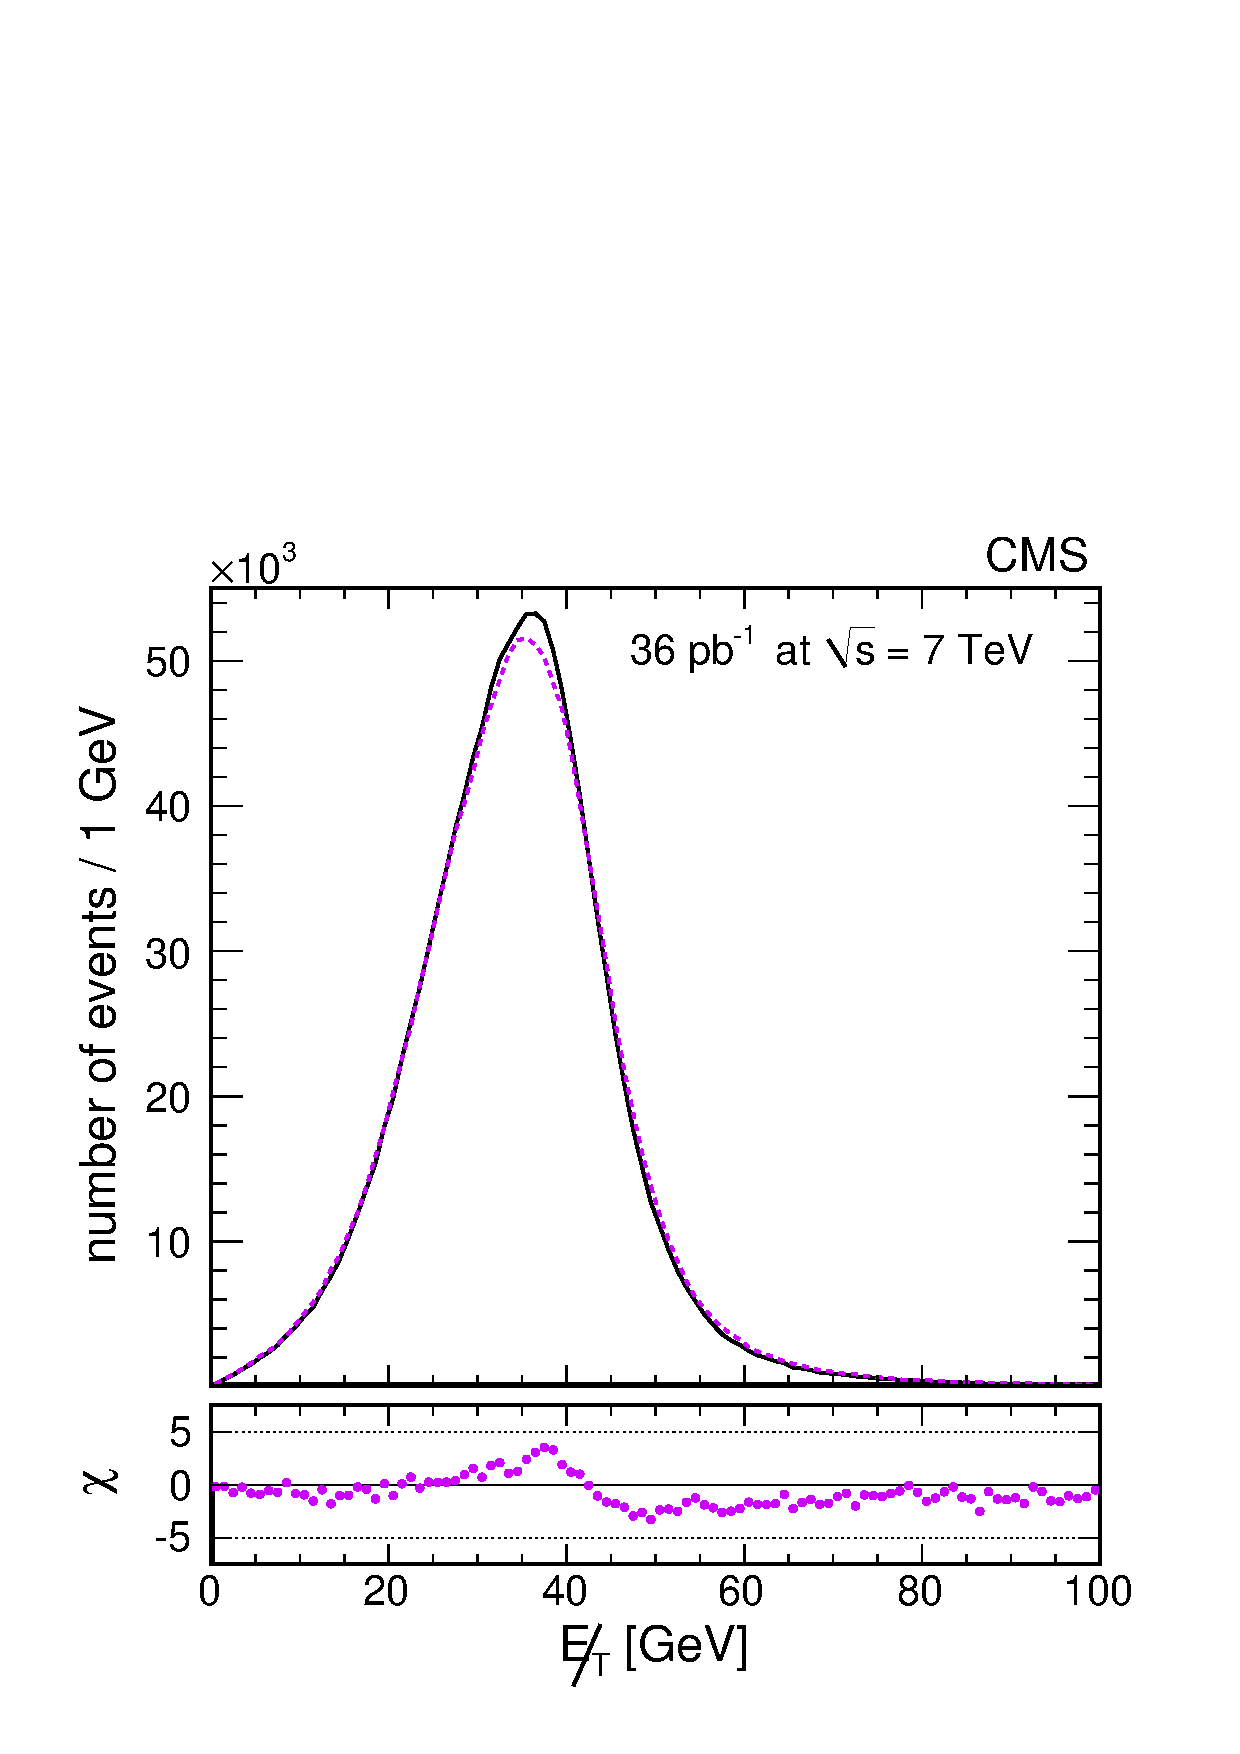
\includegraphics[width=0.48\textwidth]{figs/beforeANDafter.pdf}
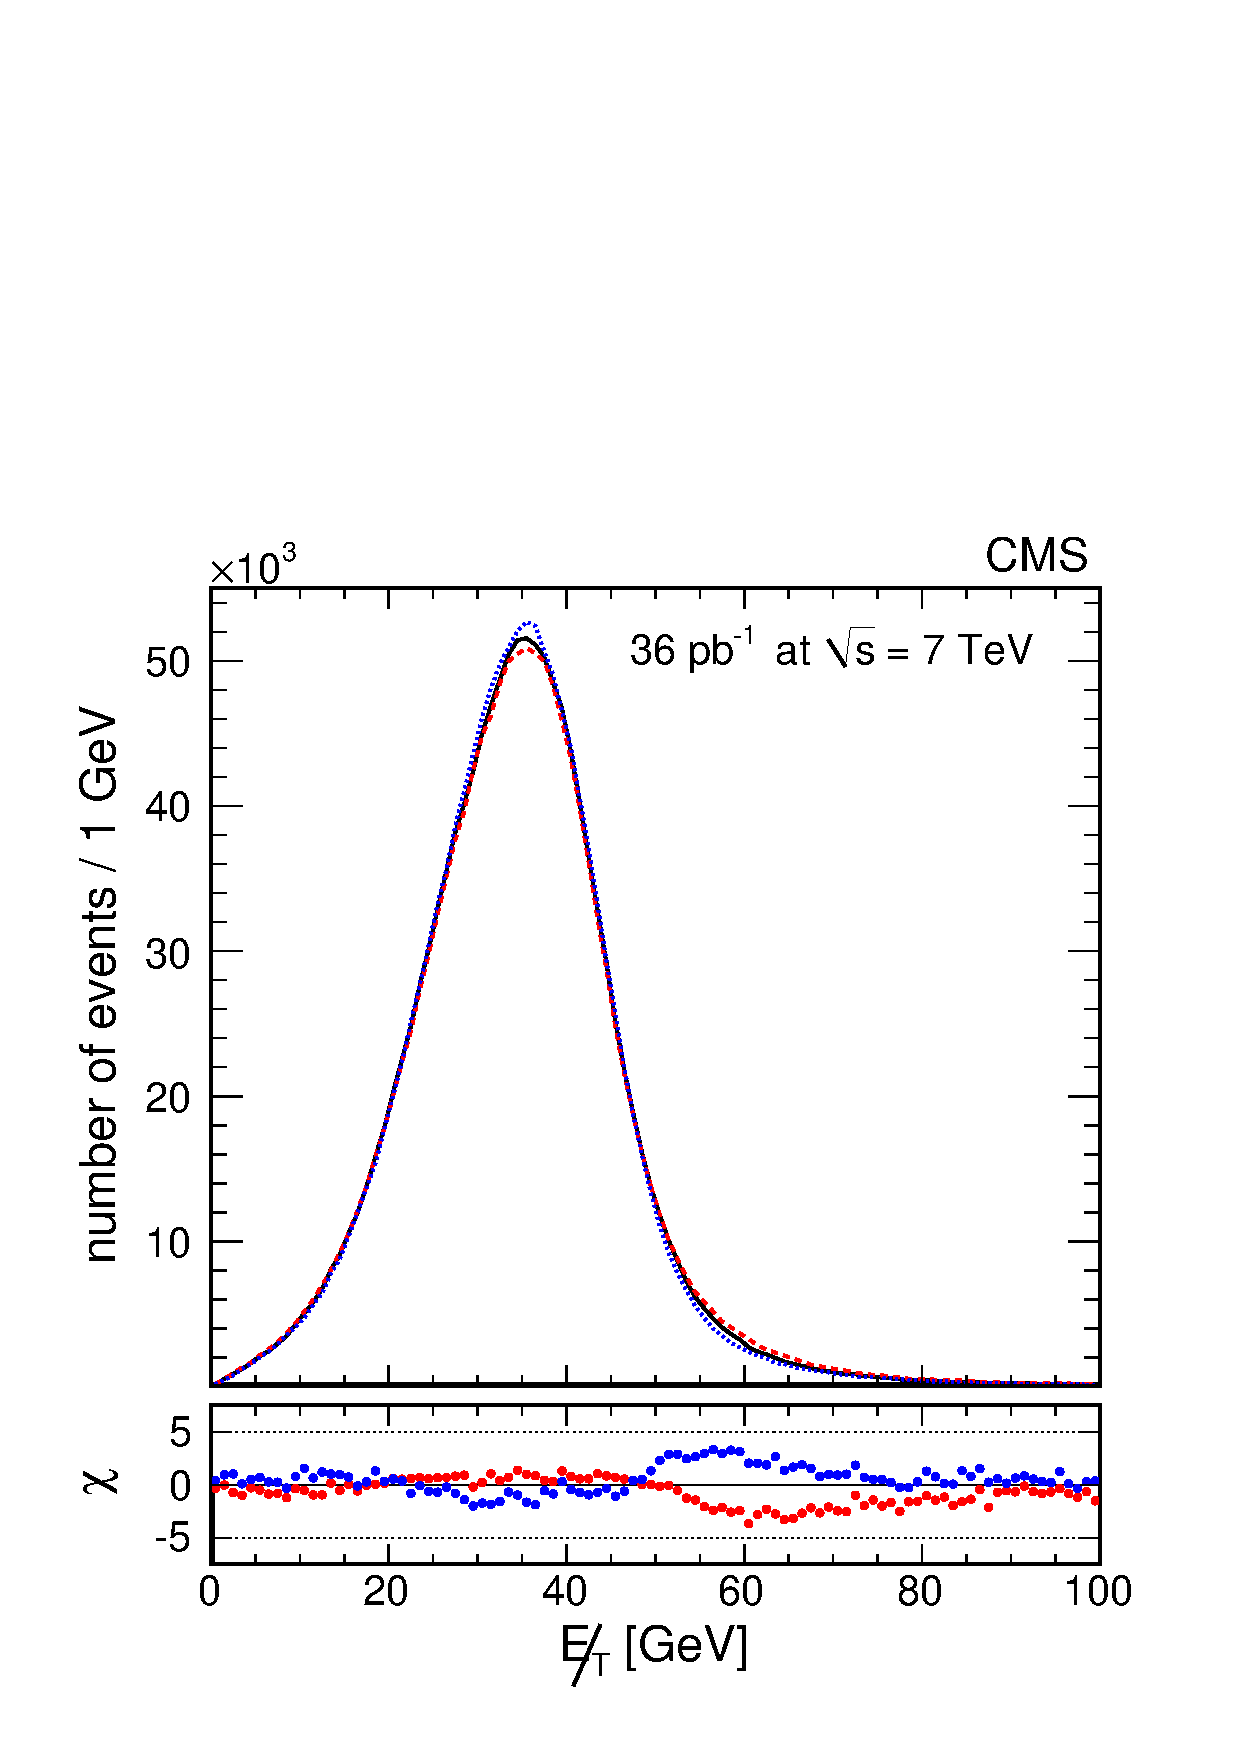
\includegraphics[width=0.48\textwidth]{figs/upANDdown.pdf}
\caption{ \label{fig:Recoil}
Left: simulated $\MET$ distribution in $\Wen$ events before (continuous black line)
and after (dashed red line) recoil corrections.
Right: the uncertainties from the recoil method propagated
to the corrected $\MET$ shape of $\Wen$ events (continuous black line, identical to the dashed
red line on the left-hand side plot) are presented with the red-dashed and blue-dotted lines.
These two shapes are obtained when the recoil systematic uncertainties are varied
by one standard deviation.
At the bottom of each plot is shown the distribution of the residuals, $\chi$, defined
as the per-bin difference of the two distributions, divided by the
corresponding statistical uncertainty.
}
\end{center}
\end{figure}
%%%%%%%%%%%%%%%%%%%%%%%%%


\subsection{Electroweak Backgrounds}
\label{sec:EWKbkgds}

A certain fraction of the events passing the selection criteria for $\Wln$
are due to other EWK processes. Several sources of
contamination have been identified. The events with $\Zll$ 
(DY background), where one of the two leptons lies
beyond the detector acceptance and escapes
detection, mimic the signature of $\Wln$ events. Events from $\Ztt$ and $\Wtn$,
with the tau decaying leptonically, have in general a lower-momentum lepton than signal
events and are strongly suppressed by the minimum $\Pt$ requirements.

The $\MET$ shape for the EWK vector boson and ${\mathrm t}\bar{\mathrm t}$ contributions are
evaluated from simulations. For the main EWK backgrounds ($\Zll$ and $\Wtn $), the $\MET$ shape is 
corrected by means of the procedure described in Section~\ref{sec:WsignalMETtemplate}.
The $\MET$ shapes are evaluated separately for $\Wptn$ and $\Wmtn$.

A summary of the background fractions in the $\Wen$ and $\Wmn$ analyses can be found in Table~\ref{tab:WlnBG}.
The fractions are similar for the $\Wen$ and $\Wmn$ channels, 
except for the DY background which is higher in the $\Wen$ channel. 
The difference is mainly due to the tighter definition of the DY veto in the $\Wmn$ channel, 
which is not compensated by the larger geometrical acceptance of electrons 
($|\eta|<2.5$) with respect to muons ($|\eta|<2.1$).
% with respect to $\Wen$ channel (the electron analysis rejects an event 
%if there is a second electron with $\Et>20.0\GeV$ while the muon analysis 
%rejects an event if there is a second muon with $\Pt>10\GeV$).

\begin{table} %
\begin{center}
\caption{\label{tab:WlnBG}
Estimated background-to-signal ratios in the $\Wen$ and $\Wmn$ channels.}

\begin{tabular}{|l|c|c|}
\hline
{\multirow{2}{*}{Processes}} & \multicolumn{2}{c|}{Bkg. to sig. ratio}  \\ \cline{2-3}
                           & $\Wen$ & $\Wmn$ \\ 
\hline \hline
$\Zee,\, \mu^+\mu^-,\, \tau^+\tau^-$ (DY)               & 7.6\%  &  4.6\% \\
$\Wtn $                    & 3.0\%  & $3.0$\%    \\
$\Wo\Wo$+$\Wo\Zo$+$\Zo\Zo$ & 0.1\% & $0.1$\%   \\
$\ttbar$                   & 0.4\% & $0.4$\%   \\
\hline
Total EWK                  & 11.2\%& $8.1$\% \\
\hline
\end{tabular}
\end{center}
\end{table}

%In the fit procedure described in the following Section, the relative normalization of the 
%EWK backgrounds is kept fixed to the values shown in Table~\ref{tab:WlnBG}.

% \begin{table}
% \begin{center}
% \begin{tabular}{|l|c|c|}
% \hline
% source & $\Nbg/(N_\Wo+\Nbg)$ & $\Nbg$ in $36.$~pb$^{-1}$ \\
% \hline\hline
% QCD multi-jet            & $5.1$\% & 8896  \\
% \hline
% $\Wtn$                   & $2.7$\%  &  4667  \\
% $\Ztt$                   & $0.5$\%  &   911  \\
% $\Wo\Wo$+$\Wo\Zo$+$\Zo\Zo$           & $0.1$\%  &   205  \\
% $\ttbar$                 & $0.3$\%  &   592  \\
% \hline
% EWK + $\ttbar$           & $7.1$\%  &  12538 \\
% \hline
% total                    & $12.2$\% &  21434 \\
% \hline
% $\Wmn$ signal            & $87.8$\%  & 153940 \\
% \hline
% \end{tabular}
% \caption{Estimates of backgrounds in the $\Wmn$ channel, based on Monte Carlo simulations.}
% \label{table:WmnBG}
% \end{center}
% \end{table}






\subsection{\texorpdfstring{Modeling of the QCD Background and $\Wen$ Signal Yield}{Modeling of the QCD Background and W-> e nu Signal Yield}}
\label{sec:WQCDbkg}

Three signal extraction methods are used, which give consistent
signal yields. The method described in Section~\ref{sec:AnalyticalFunction}
is used to extract the final result.

\subsubsection{Modeling the QCD Background Shape with an Analytical Function}
\label{sec:AnalyticalFunction}

The $\Wen$ signal is extracted using an unbinned maximum likelihood
(UML) fit to the $\MET$ distribution.
%Signal and EWK background
%distributions are derived from simulation and are validated using dedicated studies.

The shape of the $\MET$ distribution for the QCD background is modeled by a parametric function (modified Rayleigh
distribution) whose expression is
\begin{equation}
f_{\mathrm{CQD}}(\MET) = \MET\exp\left(-\frac{\MET{^2}}{2(\sigma_0+\sigma_1 \MET)^{2}}\right)\,.
\label{eq:rayleigh}
\end{equation}
The fit to a control sample, defined by inverting the track-cluster matching selection
variables $\Delta\eta$, $\Delta\phi$, shown in Fig.~\ref{fig:e-inverted}, illustrates
the quality of the description of the background shape by the parameterized function,
including the region of the signal, at high \MET.
\begin{figure}[htbp]
\begin{center}
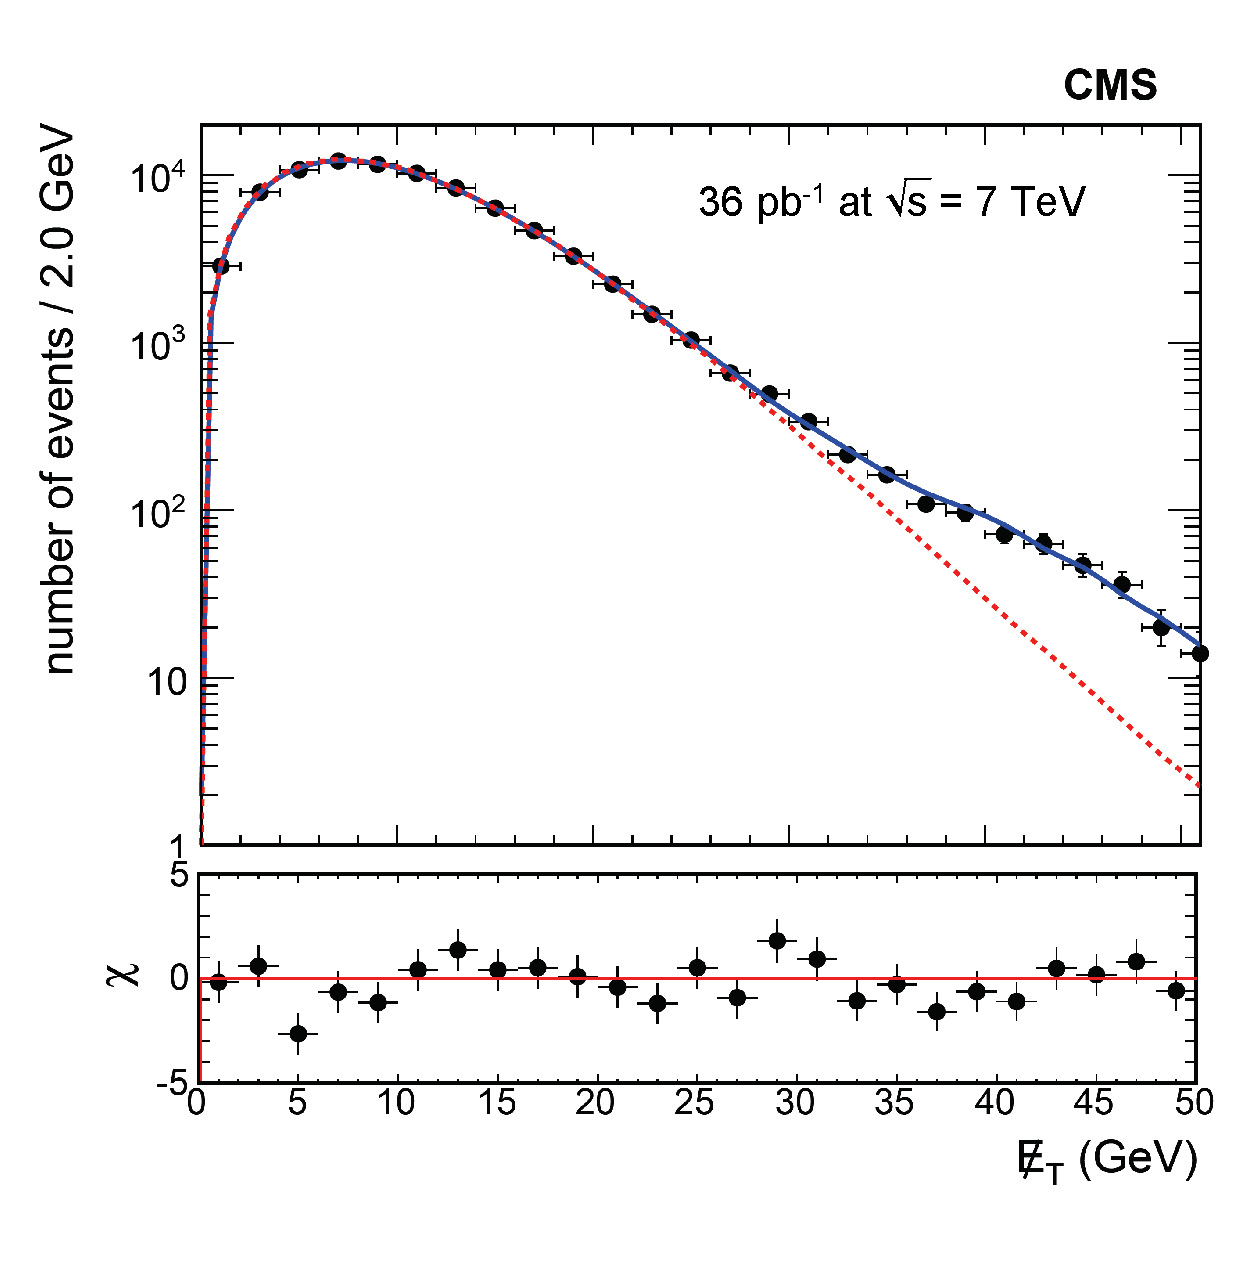
\includegraphics[width=0.50\textwidth]{figs/fixedMCyield_normal_model.pdf}
\caption{Fit to the background-dominated control sample defined by inverting
the selection on the track-match variables,
while maintaining the rest of the signal selection.
The blue solid line represents the model used to fit the control data sample. This is a Rayleigh
function plus a floating-yield signal shape that accounts for the signal contamination in the
control region. The magenta dashed line shows the Rayleigh function alone with its parameters estimated
from the combined fit.
}\label{fig:e-inverted}
\end{center}
\end{figure}
To study the systematic uncertainties associated with the background shape, the resolution term in
Eq.~(\ref{eq:rayleigh}) was changed by introducing an additional QCD shape parameter $\sigma_2$,
thus: $\sigma_0 + \sigma_1 \MET + \sigma_2 \MET^2$.

The free parameters of the UML fit are the QCD background yield,
the $\Wo$ signal yield, and the background shape
parameters $\sigma_0$ and $\sigma_1$.
The following signal yields are obtained:
$\WEIYIELD$ for the inclusive sample, $\WEPYIELD$ for the $\Wpen$ sample, and
$\WEMYIELD$ for the $\Wmen$ sample.
%with negligible correlation between the $\Wp$ and $\Wm$ yields.
The fit to the inclusive $\Wen$ sample is displayed
in Fig.~\ref{fig:Wen}, while the fits for the charge-specific
channels are displayed in Fig.~\ref{fig:WenPM}.

\begin{figure}[htbp]
\begin{center}
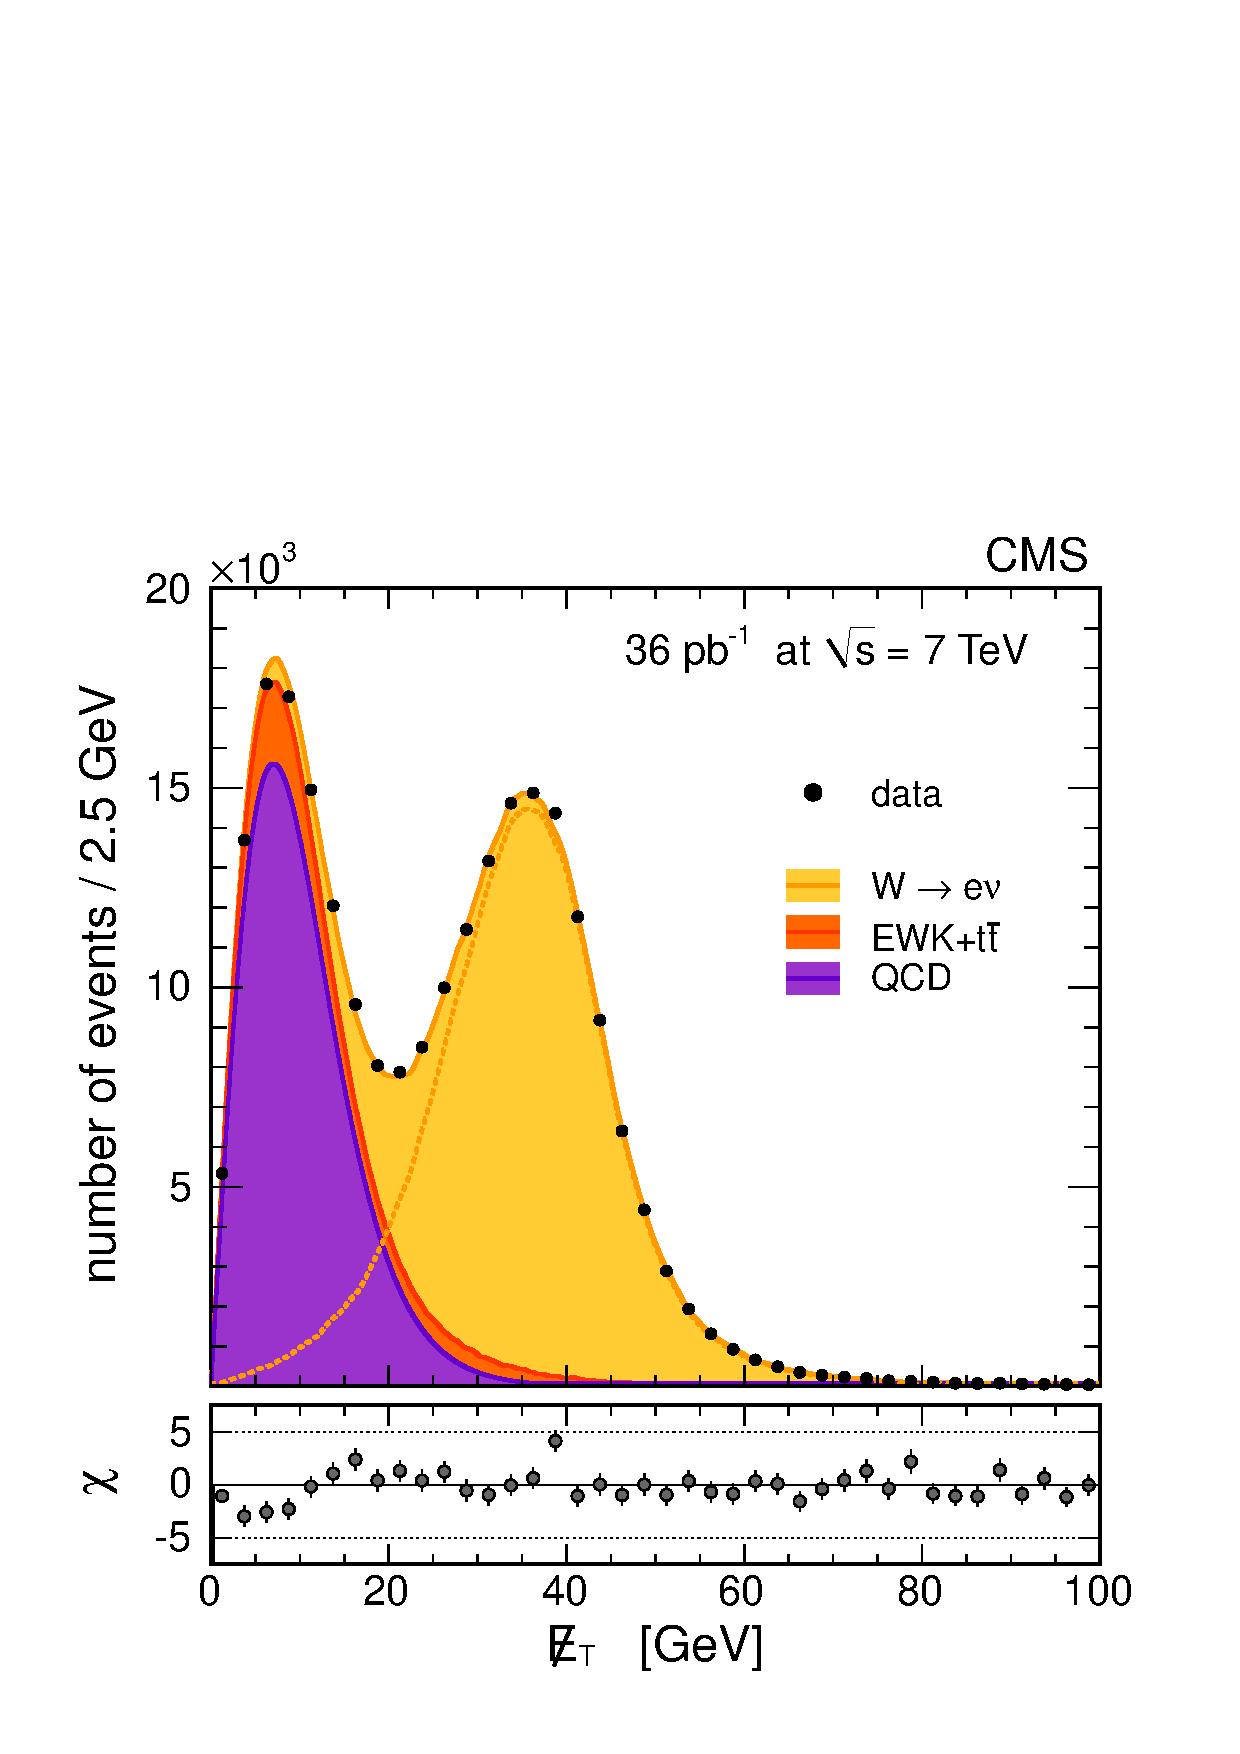
\includegraphics[width=0.48\textwidth]{figs/w_inc_36pb.pdf}
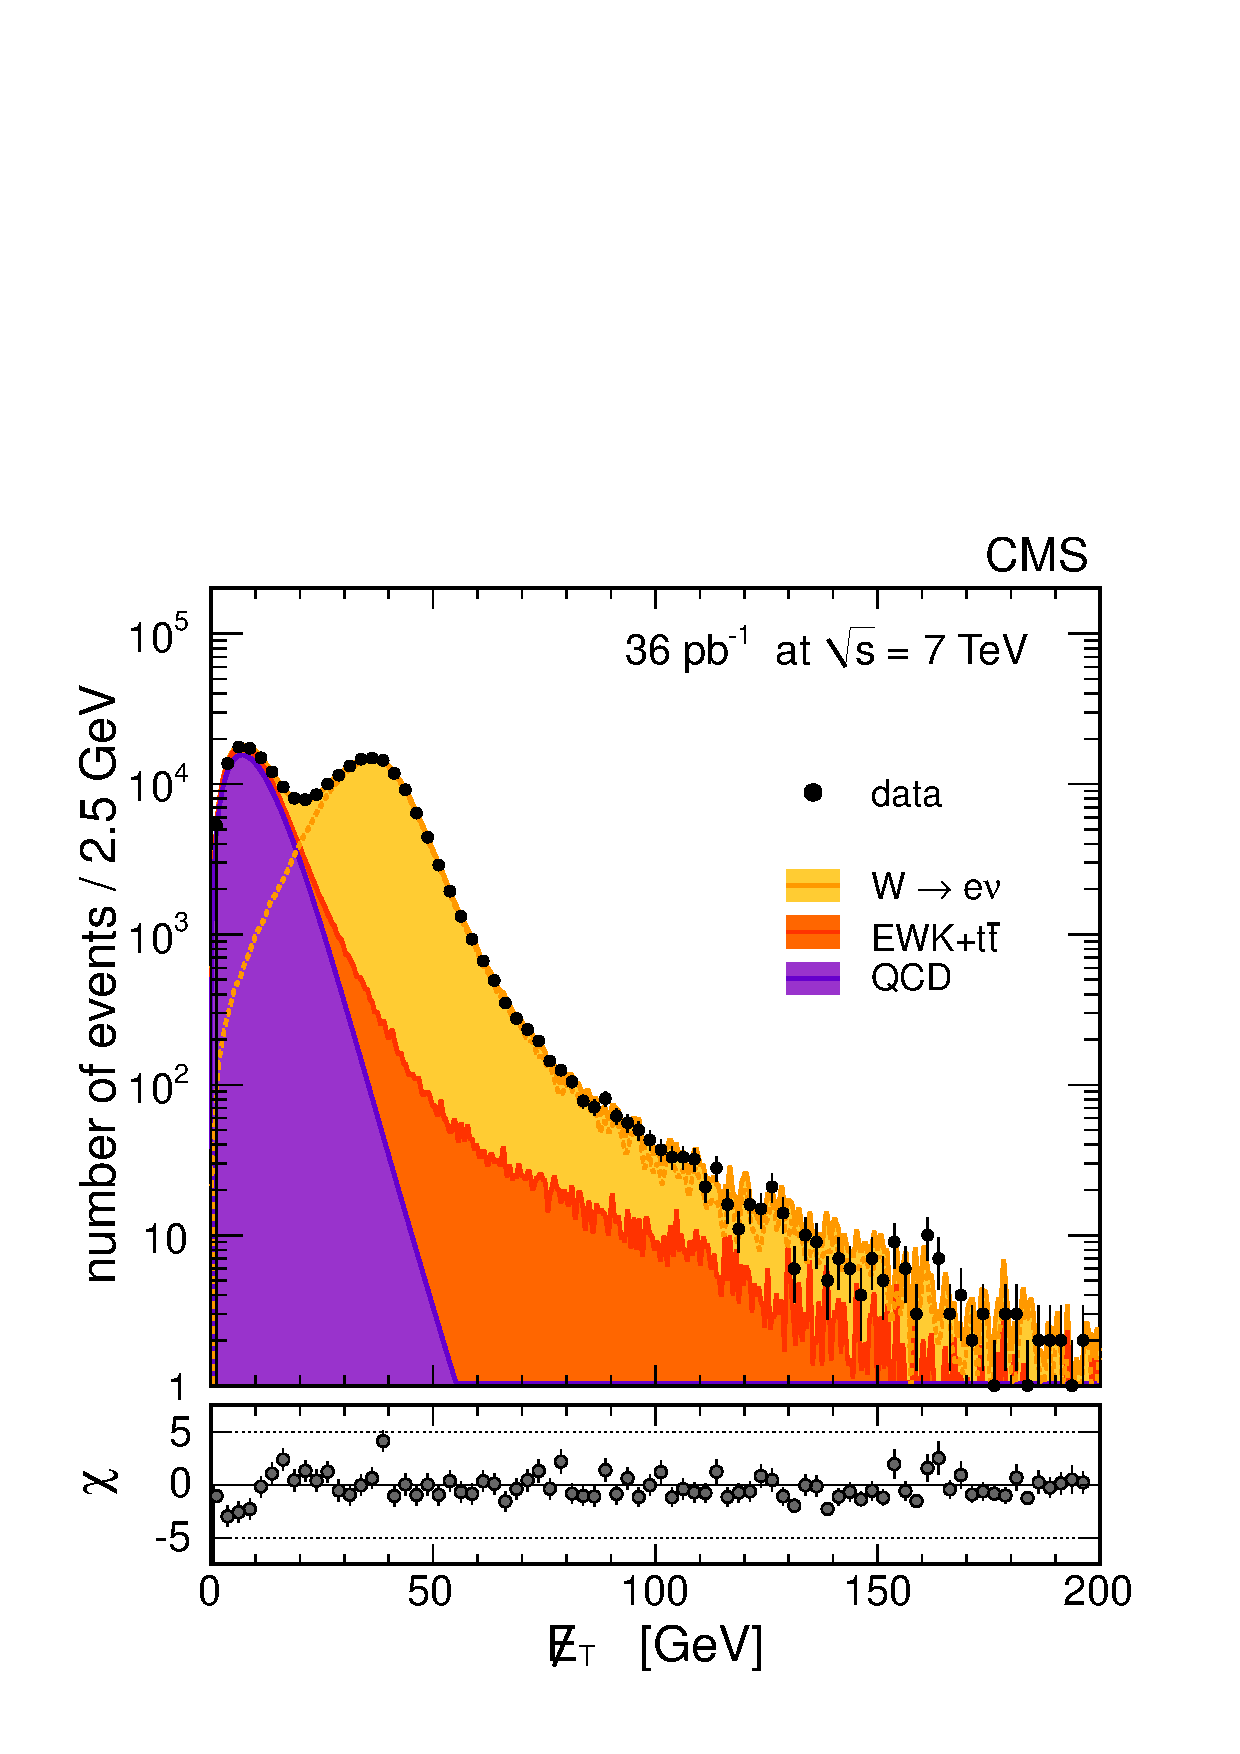
\includegraphics[width=0.48\textwidth]{figs/w_inc_36pb_log.pdf}
\caption{ \label{fig:Wen}
The $\MET$ distribution for the selected $\Wen$ candidates on
a linear scale (left) and on a logarithmic scale (right).
The points with the error bars represent the data. Superimposed are the
contributions obtained with the fit
for QCD background (violet, dark histogram), all other backgrounds
(orange, medium histogram), and signal plus  background (yellow, light histogram).
The orange dashed line is the fitted signal contribution.
}
\end{center}
\end{figure}

\begin{figure}[htbp]
\begin{center}
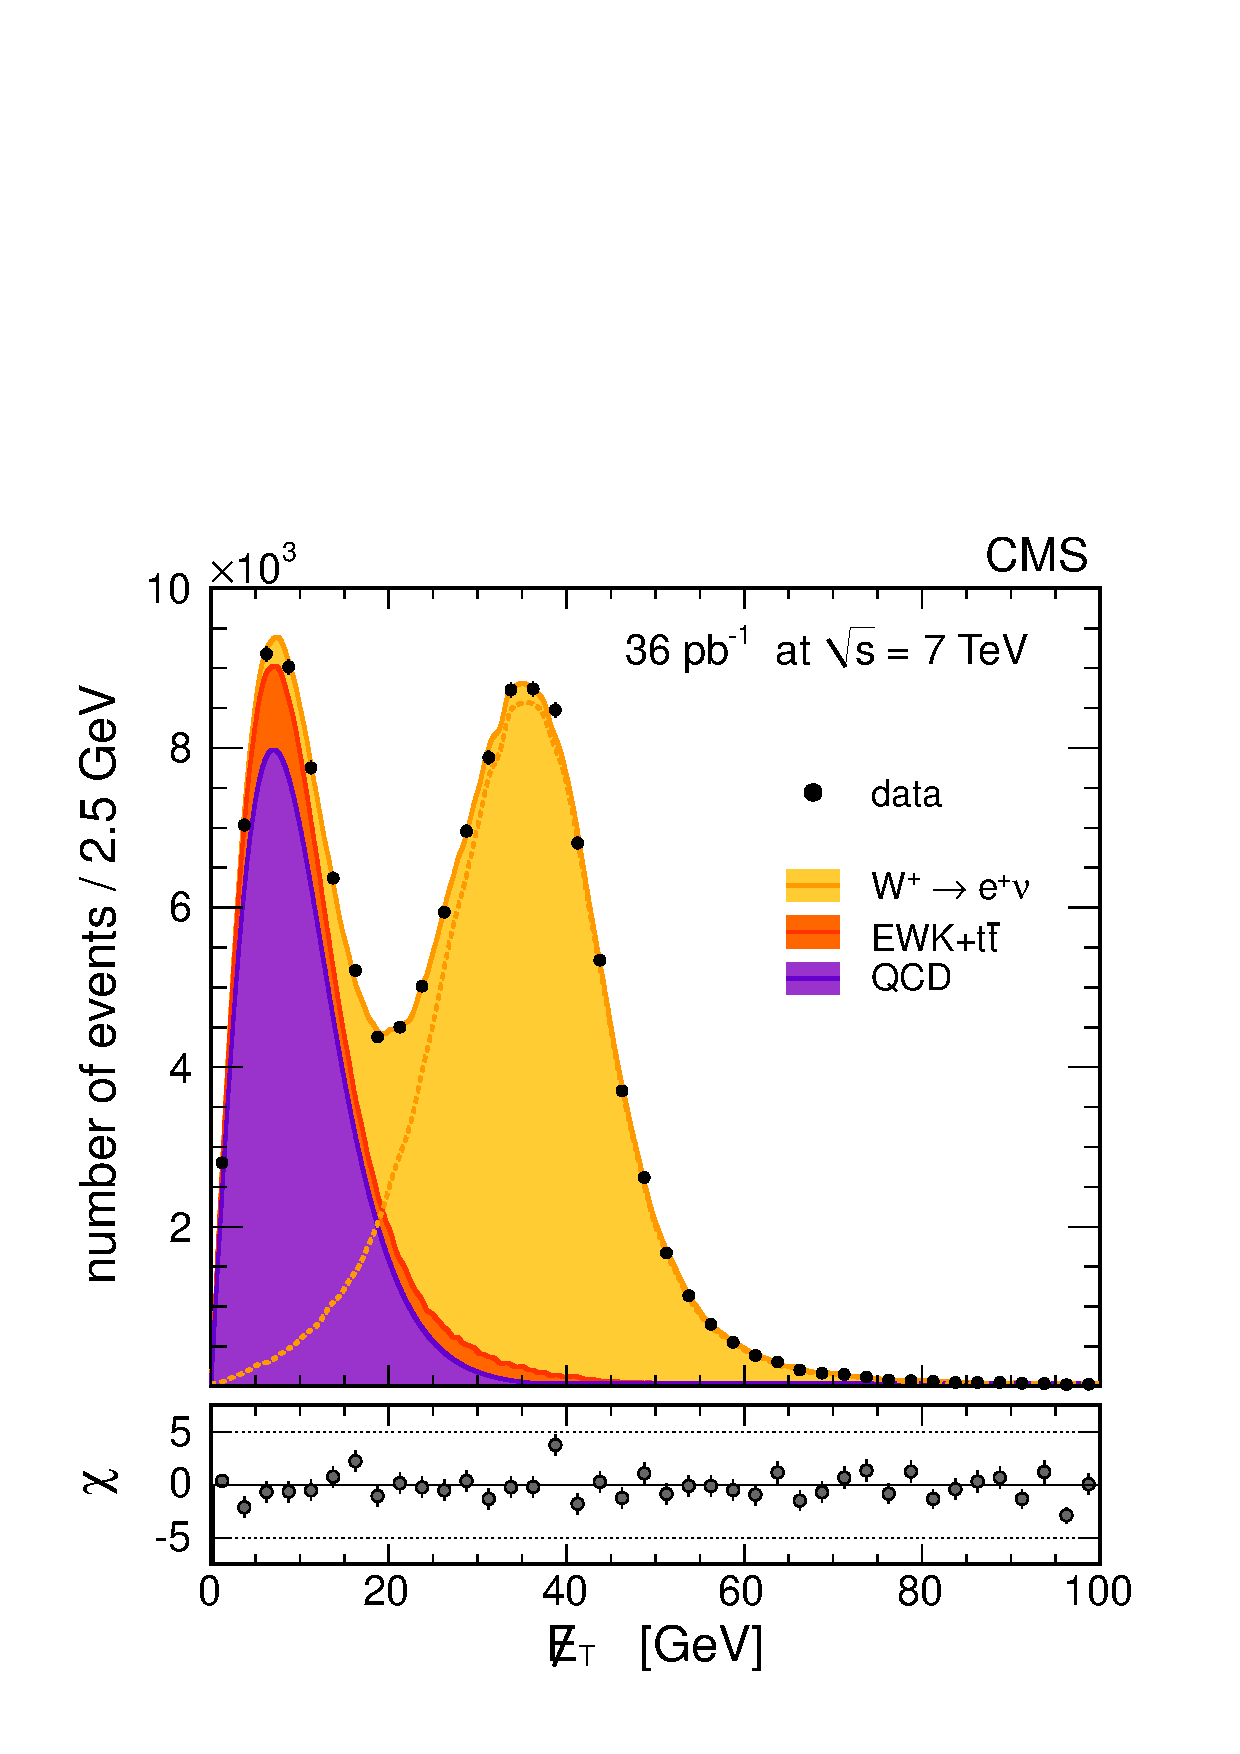
\includegraphics[width=0.48\textwidth]{figs/wp_36pb.pdf}
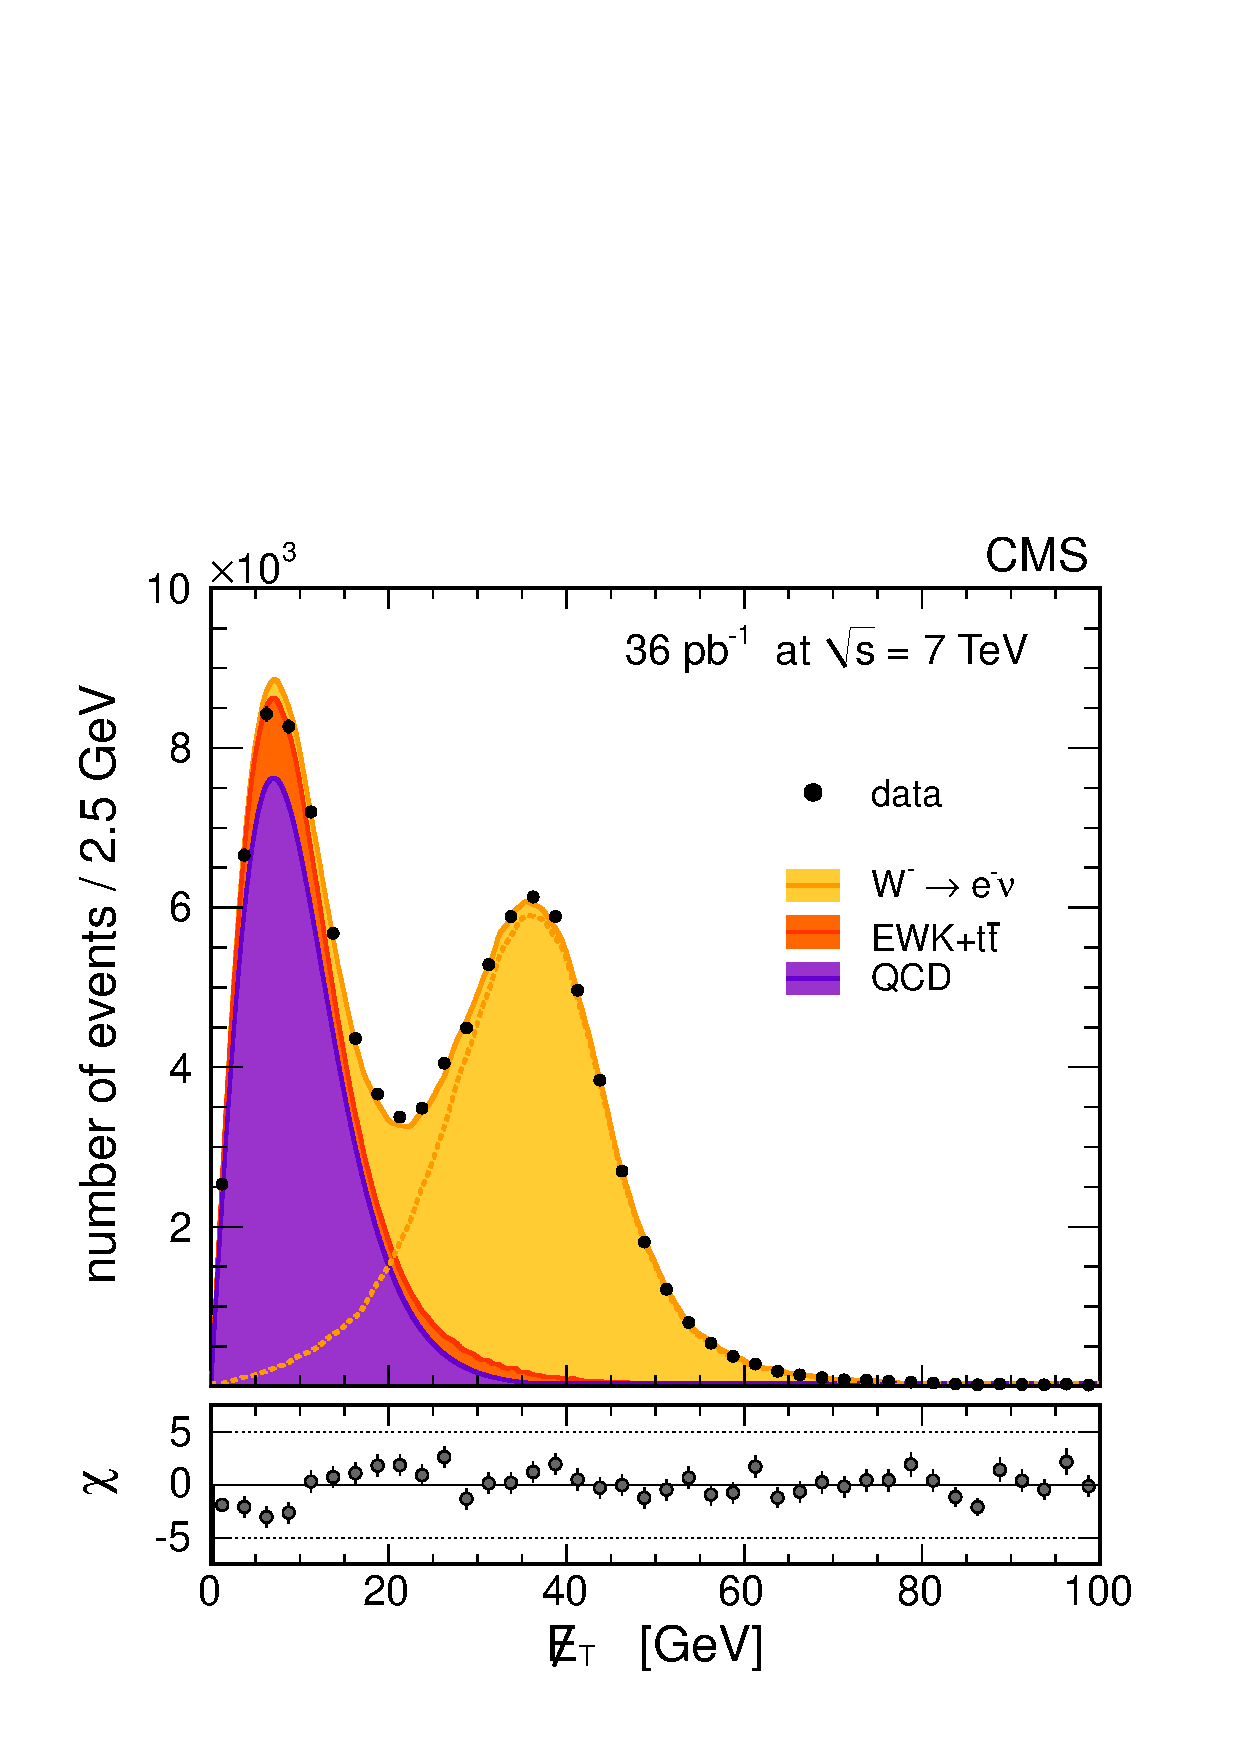
\includegraphics[width=0.48\textwidth]{figs/wm_36pb.pdf}
\caption{ \label{fig:WenPM}
The $\MET$ distributions for the selected W$^+$ (left) and W$^-$ (right) candidates.
The points with the error bars represent the data. Superimposed are the contributions
obtained with the fit for QCD background (violet, dark histogram), all other backgrounds
(orange, medium histogram), and signal plus background (yellow, light histogram).
The orange dashed line is the fitted signal contribution.
}
\end{center}
\end{figure}

The Kolmogorov--Smirnov probabilities for the fits to the charge-specific
channels are $\WEPKSPCOR$ for the $\Wp$ sample and
$\WEMKSPCOR$ for the $W^-$ sample.
\begin{figure}[t!]
\begin{center}
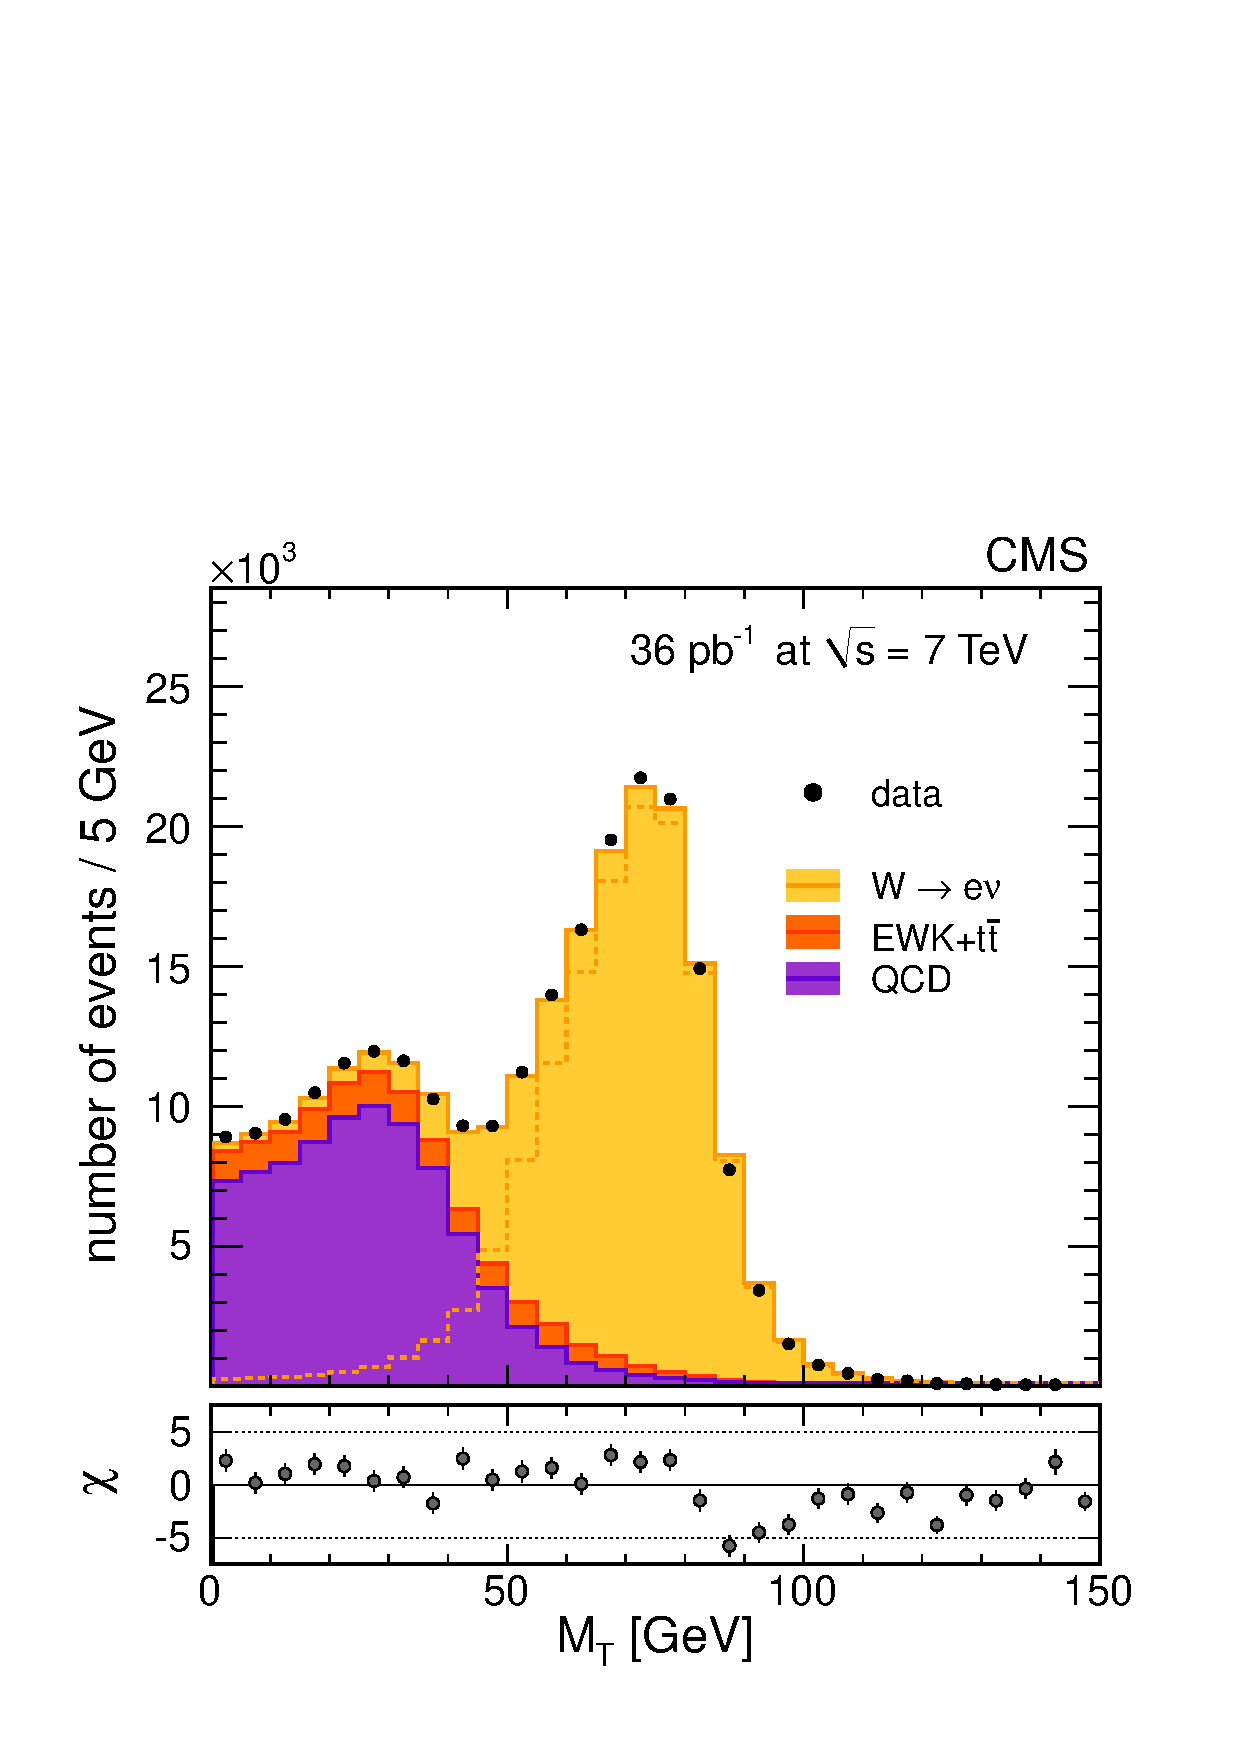
\includegraphics[width=0.48\textwidth]{figs/inc_pfmt_withMVA.pdf}
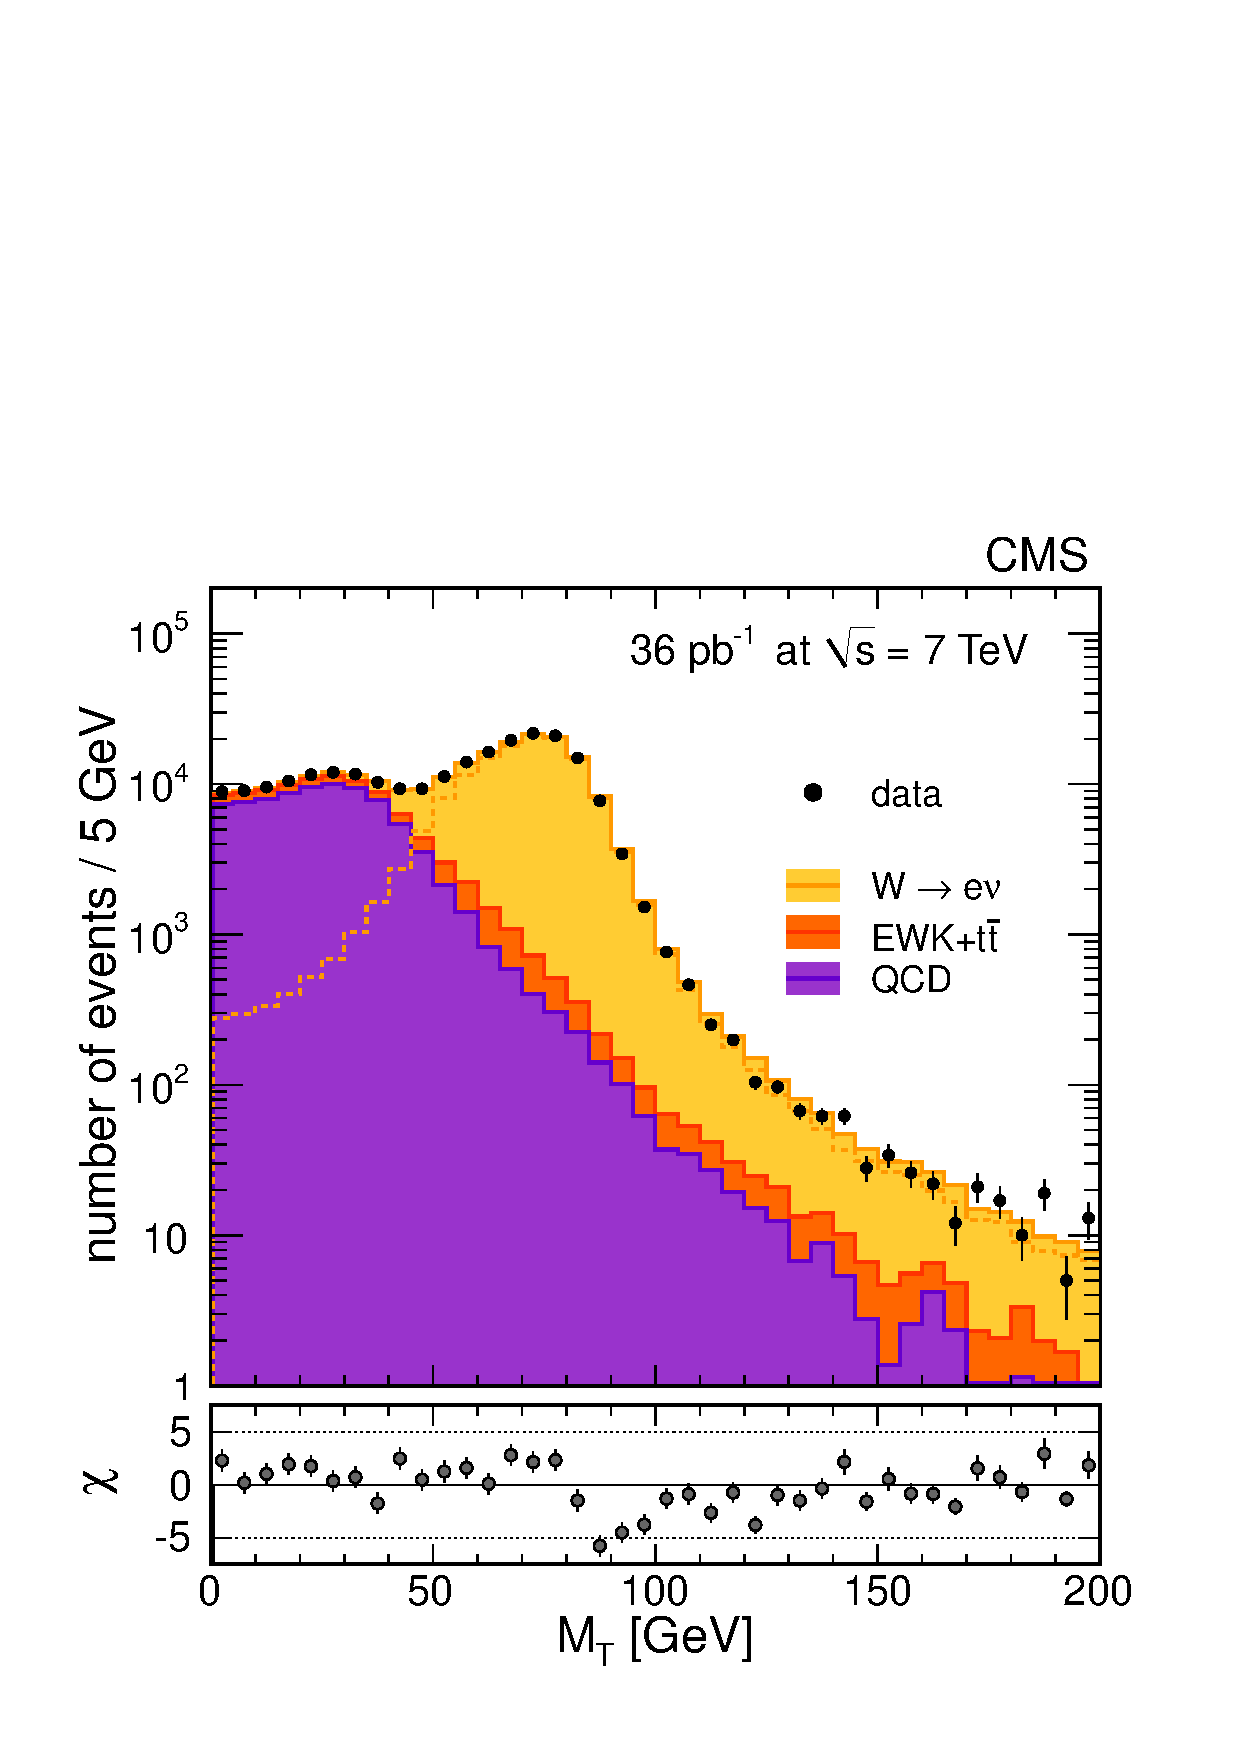
\includegraphics[width=0.48\textwidth]{figs/inc_pfmt_log_withMVA.pdf}
\caption{ \label{fig:WenMT}
The $\MT$ distribution for the selected $\Wen$ candidates on
a linear scale (left) and on a logarithmic scale (right).
The points with the error bars represent the data. Superimposed are the
contributions obtained with the fit
for QCD background (violet, dark histogram), all other backgrounds
(orange, medium histogram), and signal plus  background (yellow, light histogram).
The orange dashed line is the fitted signal contribution.
}
\end{center}
\end{figure}
Figure~\ref{fig:WenMT} shows the distribution for the inclusive $\Wo$ sample
of the transverse mass, defined as
$\MT=\sqrt{2\Pt\MET (1-\cos(\Delta\phi_{\mathrm{l},\MET}))}$,
where $\Delta\phi_{\mathrm{l},\MET}$ is the azimuthal angle between the
lepton and the $\MET$ directions.

\subsubsection{Modeling the QCD Background Shape with a Fixed Distribution}
\label{sec:e-Wsigextr-FixedTemplate}

In this approach the QCD shape is extracted directly from data using a 
control sample obtained by inverting a subset of the requirements used to select the 
signal. After fixing the shape from data,
only the normalization is allowed to float in the fit.  

The advantage of this approach 
is that detector effects, such as anomalous signals in the ca\-lo\-ri\-me\-ters or 
dead ECAL towers, are automatically reproduced in the QCD shape, since these 
effects are not affected by the selection inversion used to define the control sample.
The track-cluster matching variable $\Delta\eta$ is found
to have the smallest correlation with $\MET$ and is therefore chosen as the one 
to invert in order to suppress the signal and obtain the QCD control sample.  
Requirements on isolation and $H/E$ are the same as for the signal 
selection since these variables show significant correlation with \MET. 
\begin{figure}[h!]
  \begin{center}
    \includegraphics*[angle=-90,width=0.55\textwidth]{figs/antiselShape.pdf}
    \caption{Normalised \MET distribution for QCD and $\gamma$+jet simulated 
events passing the signal selection (solid histogram) compared 
to the normalised distribution for events from all simulated samples passing
the same inverted selection criteria used to obtain the control sample in data
(dashed histogram).}
    \label{fig:antiselShape}
  \end{center}
\end{figure}

The shape of the $\MET$ distribution for QCD and $\gamma$+jet simulated 
events passing the signal selection is compared 
to the \MET distribution for a simulated control sample composed of all simulated samples (signal and 
all backgrounds, weighted according to the 
theoretical production cross sections), after applying the same anti-selection 
as in data (Fig.~\ref{fig:antiselShape}).

\begin{figure}[htb]
  \begin{center}
    \includegraphics*[width=0.5\textwidth]{figs/Wenu_pfMET_lin.pdf}
%    \includegraphics*[width=0.48\textwidth]{figs/Wenu_pfMT_lin.pdf}
    \caption{Result of the fixed-shape fit to the $\MET$ distribution for all W candidates.
The points with the error bars represent the data.   Superimposed are the results
of the maximum likelihood fit for QCD background (violet, dark histogram), other backgrounds
(orange, medium histogram), and signal plus  background (yellow, light histogram).
The orange dashed line (left plot) is the fit contribution from signal.
}
    \label{fig:resultAll}
  \end{center}
\end{figure}

The difference in the $\MET$ distributions from the signal and inverted selections
is found to be predominantly due to two effects, which can be reduced by applying corrections.
The first effect is due to a large difference in the distribution of the output of a multivariate 
analysis (MVA) used for electron identification in the PF algorithm, between the selected events 
and the control sample. The value of the MVA output determines whether an electron candidate 
is treated by the PF algorithm as a genuine electron, or as a superposition of a charged pion and 
a photon, with track momentum and cluster energy each contributing separately to $\MET$. The control 
sample contains a higher fraction of electron candidates in the latter category, resulting in a bias on 
the $\MET$ shape. A correction is derived to account for this.
The second effect comes from the signal 
contamination in the control sample. The size of the contamination (1.17$\%$) is 
measured from data, using the \TNP technique with $\Zee$  
events, by measuring the efficiency for a signal electron to pass the 
control sample selection.


The results of the inclusive fit to the $\MET$ distribution with the fixed QCD background shape
are shown in Fig.~\ref{fig:resultAll}; the only free parameters in the extended 
maximum likelihood fit are the QCD and signal yields.
By applying this second method the following yields are obtained:
$135\,982 \pm 388$ (stat.) for the inclusive sample, $81\,286 \pm 302$ (stat.) for the $\Wpen$ sample, and
$54\,703 \pm 249$ (stat.) for the $\Wmen$ sample.
%with negligible correlation between the $\Wp$ and $\Wm$ yields.
%The quoted yields are from the $\MET$ fits. 
The ratios of the inclusive, $\Wpen$, and $\Wmen$ yields between this 
method and the parameterized
QCD shape method are $0.997 \pm 0.005$, $0.997 \pm 0.005$, and $0.999 \pm 0.005$, respectively, 
considering only the uncorrelated systematic uncertainties between the two methods.



\label{sec:e-Wsigextr-ABCDE}

\subsubsection{The ABCD Method}

%A brief summary of this method follows below. 
%A detailed description can be found 
%in the supporting document~\cite{CMS_AN_2011-009}.

In this method the data are divided into four categories defined by boundaries on $\MET$ and the relative tracker 
isolation, $\ITRK/\ET$, of the electron candidate. The boundaries of the regions are chosen to minimize the overall 
statistical and systematic uncertainties on the signal yield.
Values of $\MET$ above and below the boundary of 25 GeV, together with $\ITRK/\ET$ values below 
the boundary of 0.04, define the regions A and B, respectively.
\begin{figure}[htbp]
\begin{center}
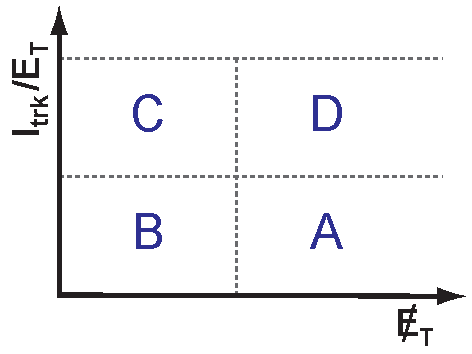
\includegraphics[width=0.35\textwidth]{figs/abcd.pdf}
\caption{The arrangement of the four categories of events used in the ABCD method. The vertical 
scale indicates increasing values of relative track isolation $\ITRK/\ET$
and the horizontal scale indicates increasing $\MET$.
%The dashed arrows show the directions of increasing signal purity.
}
\label{fig:abcde}
\end{center}
\end{figure}
Similarly, the regions above and below the $\MET$ boundary for $\ITRK/\ET$ values above 0.04, 
but below an upper $\ITRK/\ET$ bound of 0.2 (0.1) for electrons in the EB (EE), 
define the regions D and C, respectively. There is no upper bound for the $\MET$ values.
The different regions are shown graphically in Fig.~\ref{fig:abcde}, with region A 
having the greatest signal purity.
Combined regions are referred to as 'AB' (for A and B), for example.
The extracted signal corresponds to the entire ABCD region.

A system of equations is constructed relating the numbers of observed data events, $N_\mathrm{i}$, 
in each of the four regions ($\mathrm{i}$ = A, B, C and D) to the numbers 
of electroweak backgrounds, $E_\mathrm{i}$, QCD backgrounds, $Q_\mathrm{i}$, 
and signal events, $S_\mathrm{i}$. Several parameters should be determined from auxiliary 
measurements or simulations as shown in the following formulas: 

\begin{eqnarray}
 \label{eqABCD_Fa}
   f_\mathrm{A} & = & \frac{Q_\mathrm{A}}{Q_\mathrm{A} + Q_\mathrm{B}}  \\
  \label{eqABCD_Fb}
   f_\mathrm{D} & = & \frac{Q_\mathrm{D}}{Q_\mathrm{C} + Q_\mathrm{D}}  \\
  \label{eqABCD_EFFa}
   \epsilon_\mathrm{A} & = & \frac{S_\mathrm{A}}{S_\mathrm{A} + S_\mathrm{B}}  \\
  \label{eqABCD_EFFd}
   \epsilon_\mathrm{D} & = & \frac{S_\mathrm{D}}{S_\mathrm{C} + S_\mathrm{D}}  \\
  \label{eqABCD_EFFp}
   \epsilon_\mathrm{P} & = & \frac{S_\mathrm{A} + S_\mathrm{B}}{S_\mathrm{A} + S_\mathrm{B} + S_\mathrm{C} + S_\mathrm{D}} 
\end{eqnarray}

In this formulation, two parameters, $f_\mathrm{A}$ and $f_\mathrm{D}$, relate to the QCD 
backgrounds and are defined as the ratios of events with a fake electron candidate in the A and D 
regions to the number in the AB and CD regions, respectively. The two parameters represent the 
efficiency with which misidentified electrons pass the boundary on $\MET$ dividing
AD from BC. If the efficiency for passing the $\MET$ boundary is largely independent of the choice of
the boundaries on $\ITRK/\ET$, then these two parameters will be approximately equal. 
Assuming $f_\mathrm{A}=f_\mathrm{D}$ holds exactly 
leads to a simplification of the system of equations such that all direct dependence of the signal
extraction on parameters related to the QCD backgrounds is eliminated. For this idealized case there would be
no uncertainty on the extracted signal yield arising from modeling of QCD backgrounds. Detailed studies of the
data suggest this assumption holds to a good degree. A residual bias in the extracted signal arising from this
assumption is estimated directly from the data by studying a control sample 
obtained with inverted quality requirements on the electron candidate, 
and an appropriate small correction to the yield is applied (${\approx}0.37\%$).
A systematic uncertainty on the signal yield is derived from the uncertainty on this bias correction.
This contribution is small and is dominated by the uncertainty on signal
contamination in the control sample.

Three other important parameters relate to signal efficiencies: $\epsilon_\mathrm{A}$ 
and $\epsilon_\mathrm{D}$, which
are the efficiencies for signal events in the AB and CD regions, respectively, to pass the 
$\MET$ boundary, and $\epsilon_\mathrm{P}$, which is the efficiency for the electron candidate of a signal event 
to pass the boundary on relative track isolation dividing the AB region from the CD region under the 
condition that this electron already lies in the ABCD region. 
The first two of these, $\epsilon_\mathrm{A}$ and $\epsilon_\mathrm{D}$, are
estimated from models of the $\MET$ in signal events using the 
methods described in Section~\ref{sec:WsignalMETtemplate}.
The third parameter, $\epsilon_\mathrm{P}$, is measured from data using the \TNP method, described in
Section~\ref{sec:ELEefficiencies}, and is one of the dominant sources of 
uncertainty on the $\Wo$ boson yield before
considering the final acceptance corrections.

Electroweak background contributions are estimated from MC samples
with an overall normalization scaled through an iterative method with the signal yield. 
The electroweak contribution is subtracted from the observed data events in each of the four 
regions, $N_\mathrm{i} \rightarrow N_\mathrm{i} - E_\mathrm{i}$ ($\mathrm{i}$ = A, B, C and D).

Assuming that $f_\mathrm{A}$ = $f_\mathrm{B}$, the signal contained in the ABCD region, S, can 
be obtained from the following formula:

\begin{eqnarray}
 \label{eqABCD_S}
   \alpha S^2 + b S + c & = & 0 
\end{eqnarray}

with coefficients, 

\begin{eqnarray}
 \label{eqABCD_Sa}
   \alpha & = & \epsilon_\mathrm{P}(\epsilon_\mathrm{P} - 1)(\epsilon_\mathrm{A} - \epsilon_\mathrm{D})   \\
  \label{eqABCD_Sb}
   b & = & N_\mathrm{A}(1 - \epsilon_\mathrm{D})(1 - \epsilon_\mathrm{P}) - N_\mathrm{B}\epsilon_\mathrm{D}(1 - \epsilon_\mathrm{P}) + N_\mathrm{C}\epsilon_\mathrm{A}\epsilon_\mathrm{P} - N_\mathrm{D}\epsilon_\mathrm{P}(1 - \epsilon_\mathrm{A})  \\
  \label{eqABCD_Sc}
   c & = & N_\mathrm{B}N_\mathrm{D} - N_\mathrm{A}N_\mathrm{C}
\end{eqnarray}

The extracted yield with respect to the choice of boundaries in relative track isolation and $\MET$ is 
sensitive to biases in $\epsilon_\mathrm{P}$ and the QCD electron misidentification rate 
bias correction described above, respectively. 
The yield is very stable with respect to small changes in these selections, 
giving confidence that these 
important sources of systematic uncertainty are small.

The following signal yields are obtained:
$136\,003 \pm 498\,\mathrm{(stat.)}$ for the inclusive sample, $81\,525 \pm 385\,\mathrm{(stat.)}$ 
for the $\Wpen$ sample, and $54\,356 \pm 315\,\mathrm{(stat.)}$ for the $\Wmen$ sample.
%with negligible correlation between the $\Wp$ and $\Wm$ yields.
The ratios of the inclusive, $\Wpen$, and $\Wmen$ yields between this method and the parameterized
QCD shape are $0.998 \pm 0.007$, $0.999 \pm 0.007$, and $0.993 \pm 0.007$, respectively, considering
only the uncorrelated systematic uncertainties between the two methods.



The results of the three signal extraction methods are summarised in Table~\ref{tab:WsignalCollection}.

\begin{table}[htbp] %
\begin{center}
   \caption[.]{ \label{tab:WsignalCollection}
Comparison of $\Wen$ signal extraction methods. The signal yield of each method is presented together with
its statistical uncertainty.
For the fixed shape and the ABCD methods, the ratios of the signal yields with the analytical function method
are also shown taking into account only the uncorrelated systematics between the methods used in the ratios.}
\begin {tabular} {|l|l|c|c|c|}
\hline
\multicolumn{2}{|l|}{Source}        & $\Wen$           & $\Wpen$           & $\Wmen$            \\
\hline\hline
Analytical fun. &yield    & $\WEIYIELD$      &  $\WEPYIELD$      &  $\WEMYIELD$      \\
\hline
\multirow{2}{*}{Fixed shape} & yield                         & $\WEIftYIELD$    &  $\WEPftYIELD$    &  $\WEMftYIELD$      \\
 & ratio & $\rWEIftYIELD$   &  $\rWEPftYIELD$   &  $\rWEMftYIELD$      \\
\hline
\multirow{2}{*}{ABCD} & yield                                & $\WEIabYIELD$    & $\WEPabYIELD$     & $\WEMabYIELD$    \\
 & ratio       & $\rWEIabYIELD$   & $\rWEPabYIELD$    & $\rWEMabYIELD$    \\
\hline
\end {tabular}
\end{center}
\end{table}



\subsection{\texorpdfstring{Modeling of the QCD Background and $\Wmn$ Signal Yield}{Modeling of the QCD Background the W->mu nu Signal Yield}}
\label{sec:Wmunu}

The $\Wmn$ analysis is performed using fixed distributions for the $\MET$ shapes
obtained from data for the QCD background component and from simulations,
after applying proper corrections, for the signal and the remaining background components.

Different approaches to signal extraction are considered for $\Wmn$, as for $\Wen$.
The alternative methods do not demonstrate better performance than the use of fixed shapes
in the W signal fit. Given the lower backgrounds in the muon channel with respect to the
electron channel, the alternative strategies are not pursued at the same level of detail
as in the electron case.

The $\MET$ shape of the QCD background component is obtained from a high-purity QCD sample
of events that pass the signal selection, except that the isolation requirement
is inverted and set to $\IRelComb > 0.2$ (Fig.~\ref{figure:Wmunu_iso}).

Simulation studies indicate that this distribution does not accurately
reproduce the $\MET$ shape when muon isolation is required.
This is shown in Fig.~\ref{figure:Wmunu_QCD} (left),
where the solid line represents the shape for events with an isolated muon and the dashed line
the shape obtained by inverting the isolation requirement. %They are very distinct.

A positive correlation between the isolation variable $\IRelComb$ and $\MET$ is shown
in Fig.~\ref{figure:Wmunu_QCD} (right, red open circles). This behavior can be
parameterized in terms of a linear function
$\MET\propto (1+\alpha\,\IRelComb)$, as shown in the same figure.
A compensation for the correlation is subsequently made
by applying a correction of the kind of $\MET^\prime = \MET/(1+\alpha\,\IRelComb)$ to
the events selected by inverting the isolation requirement and a new corrected shape is obtained.
The agreement of this new shape (black points in Fig.~\ref{figure:Wmunu_QCD}, left)
with the prediction from events with an isolated muon is considerably improved.
It is also observed that a maximal variation in the correction factor of $\Delta \alpha =  0.08$ successfully
covers the simulation prediction for events with an isolated muon over the whole $\MET$ interval (shaded area in Fig.~\ref{figure:Wmunu_QCD}, left).
\begin{figure}[htbp] {\centering
    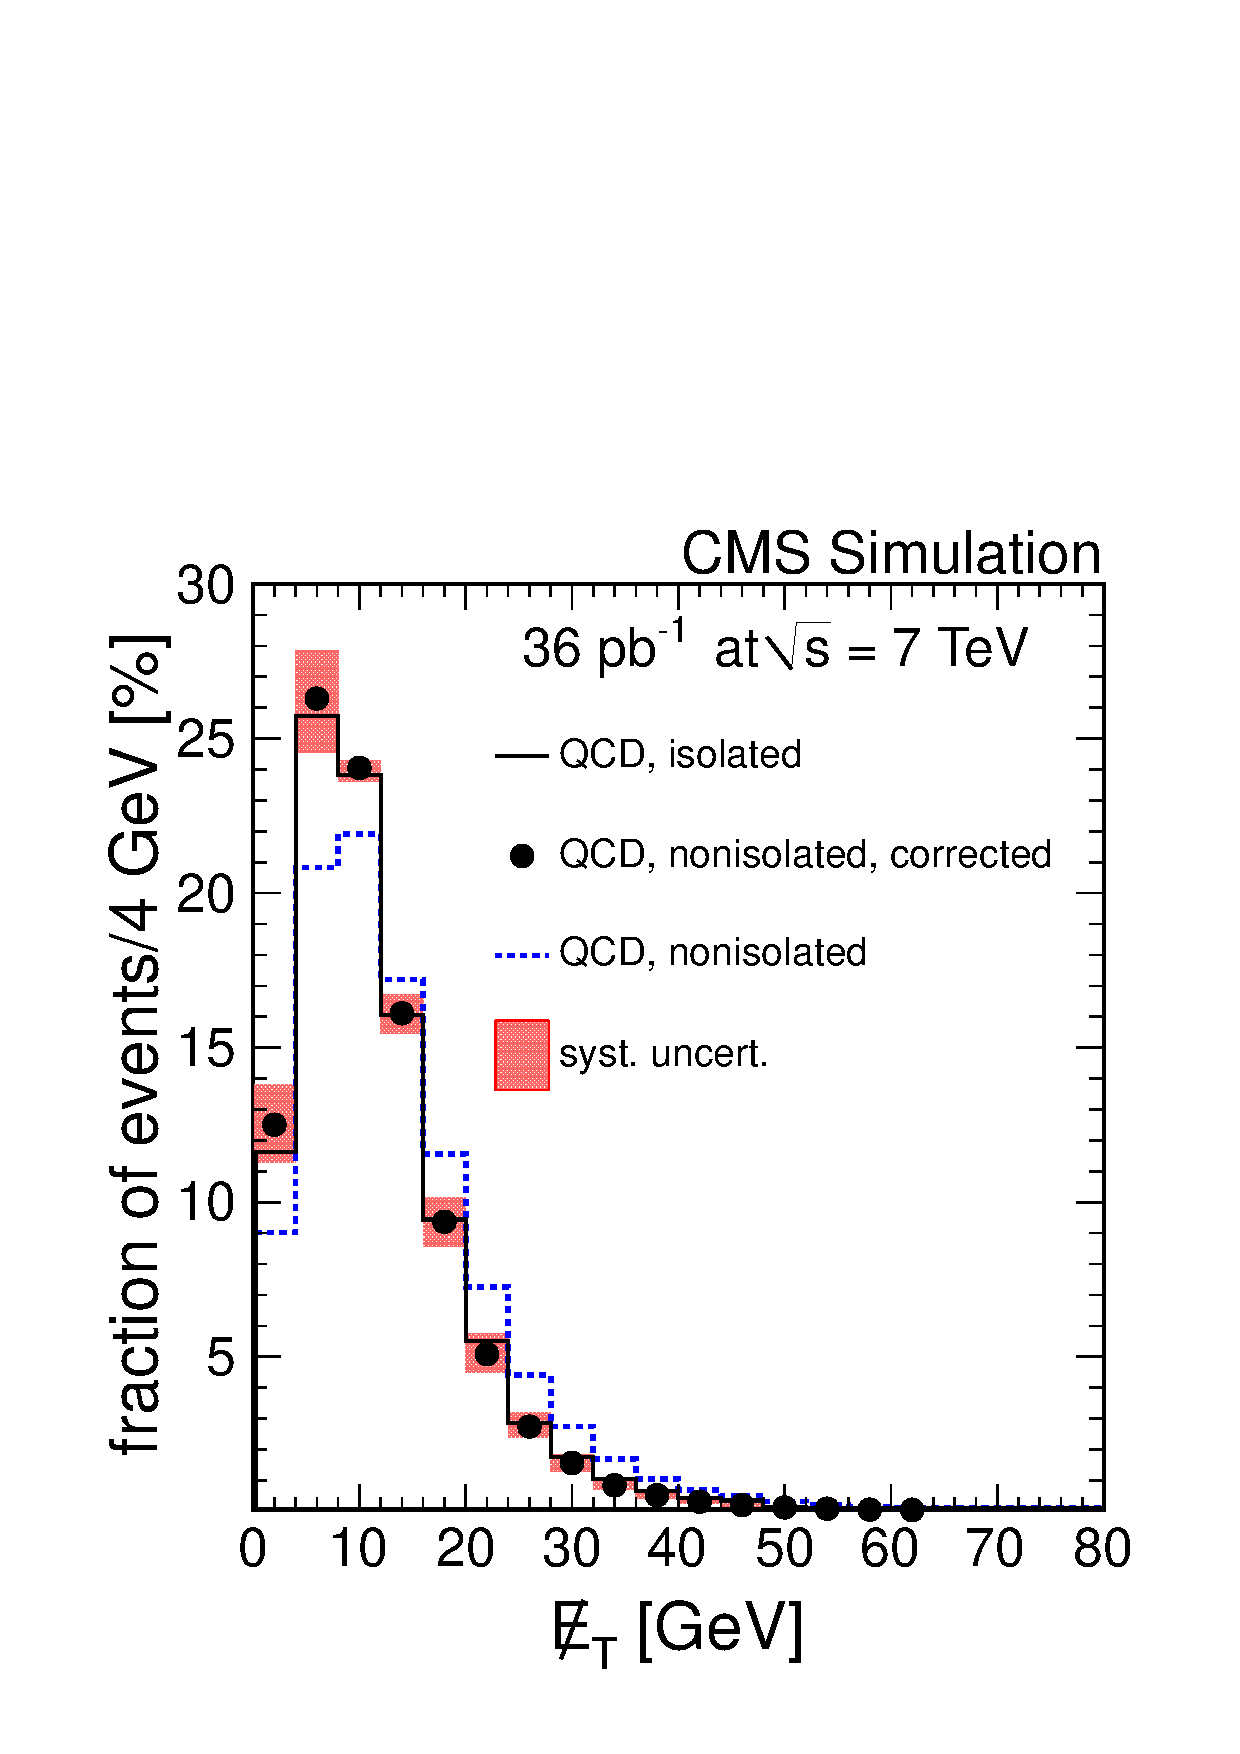
\includegraphics[width=7.5cm]{figs/qcd_template_MC.pdf}
    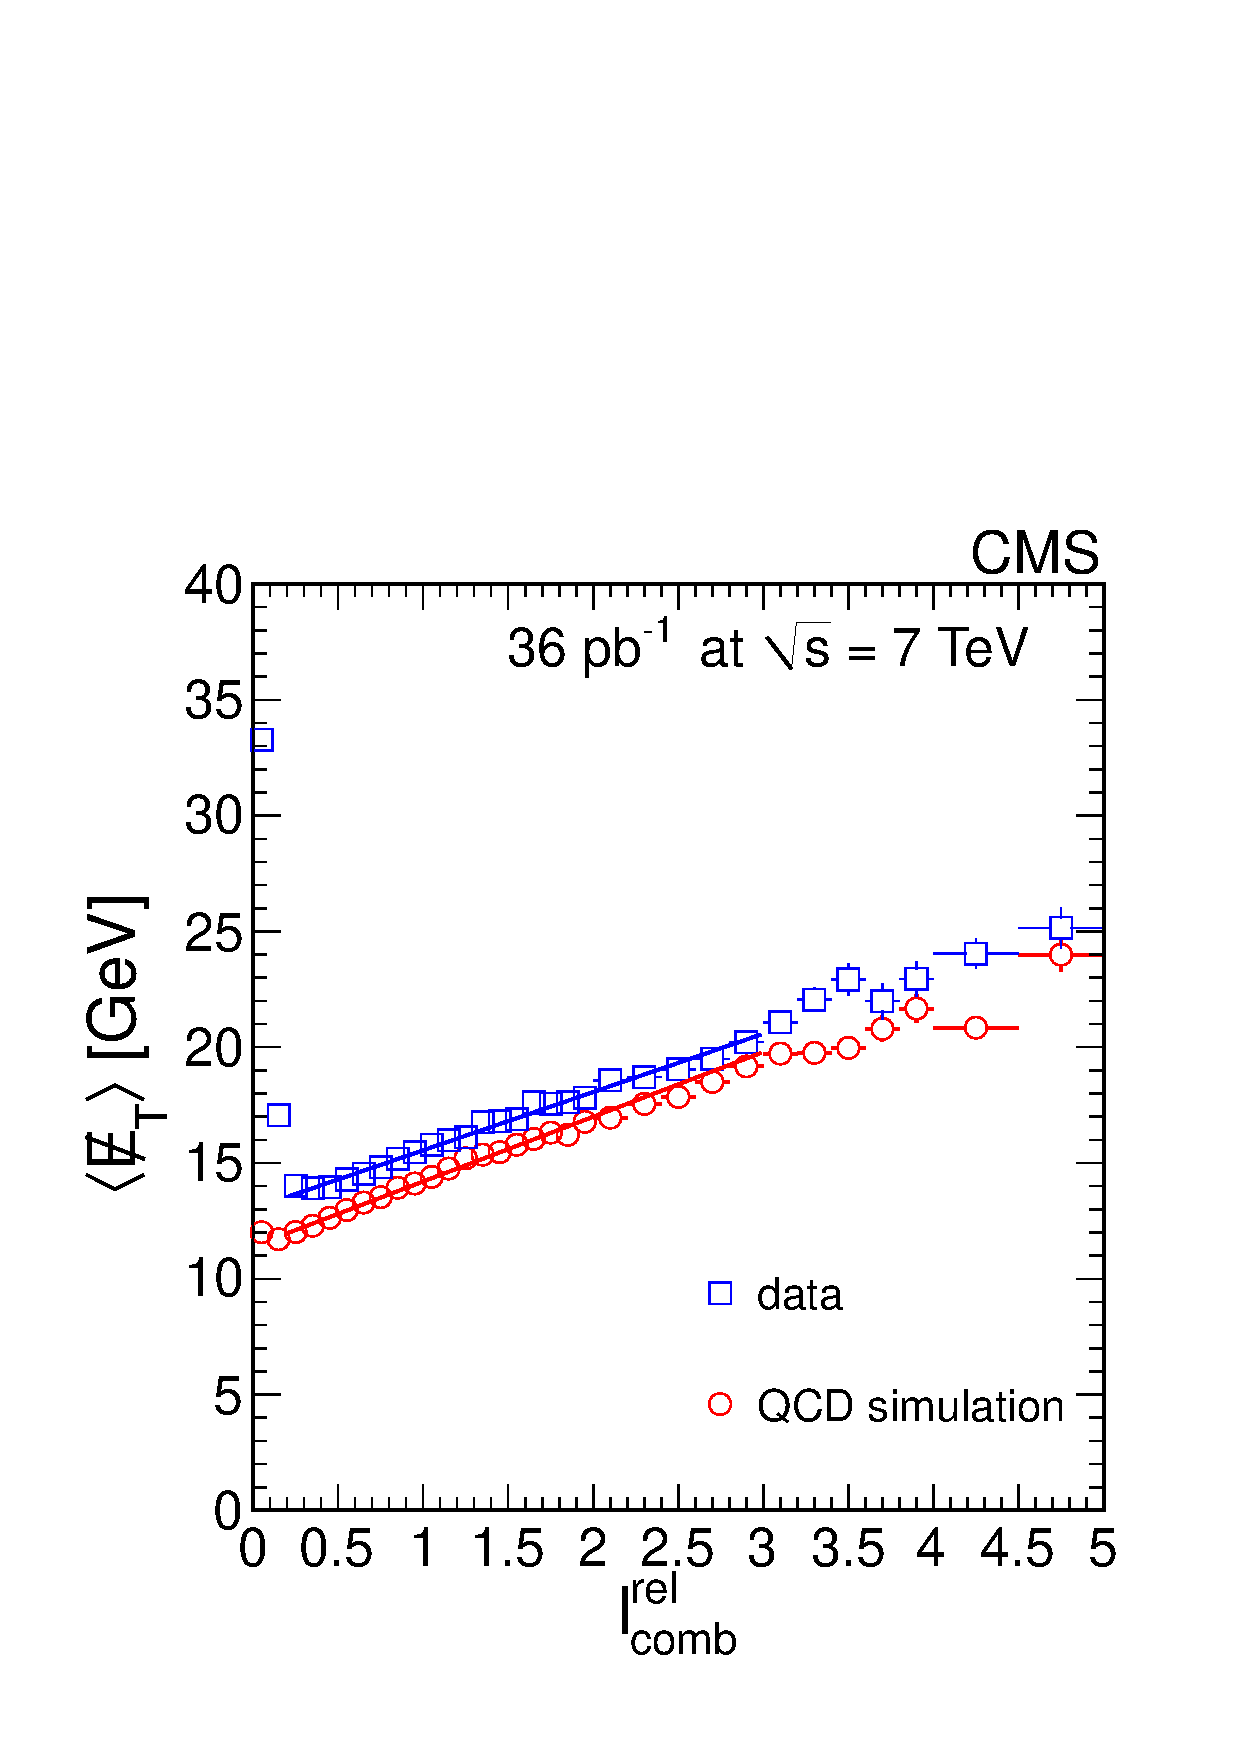
\includegraphics[width=7.5cm]{figs/Wmn_METvsIso.pdf}
    \caption{Left: distribution of the corrected $\MET$ for selected events
with a non isolated muon (black points) superimposed
on the distribution of uncorrected $\MET$ for the same events (blue, dashed line) and
$\MET$ for events with an isolated muon (black, solid histogram). All distributions are from simulated QCD events.
The shaded area represents the systematic uncertainty due to corrections
with factors $\alpha \pm \Delta \alpha$, for $\Delta \alpha = 0.08$.
Right: distribution of the average $\MET$ versus $\IRelComb$
for simulated QCD events (red circles) and
for data (blue squares).
The high values of $\MET$ in the first two bins in $\IRelComb$
are due to the presence of the W signal events. The superimposed lines are linear fits
in the range $[0.2, 3.0]$ of $\IRelComb$.
    \label{figure:Wmunu_QCD}}
}
\end{figure}
\begin{figure}[htbp]
{\centering
    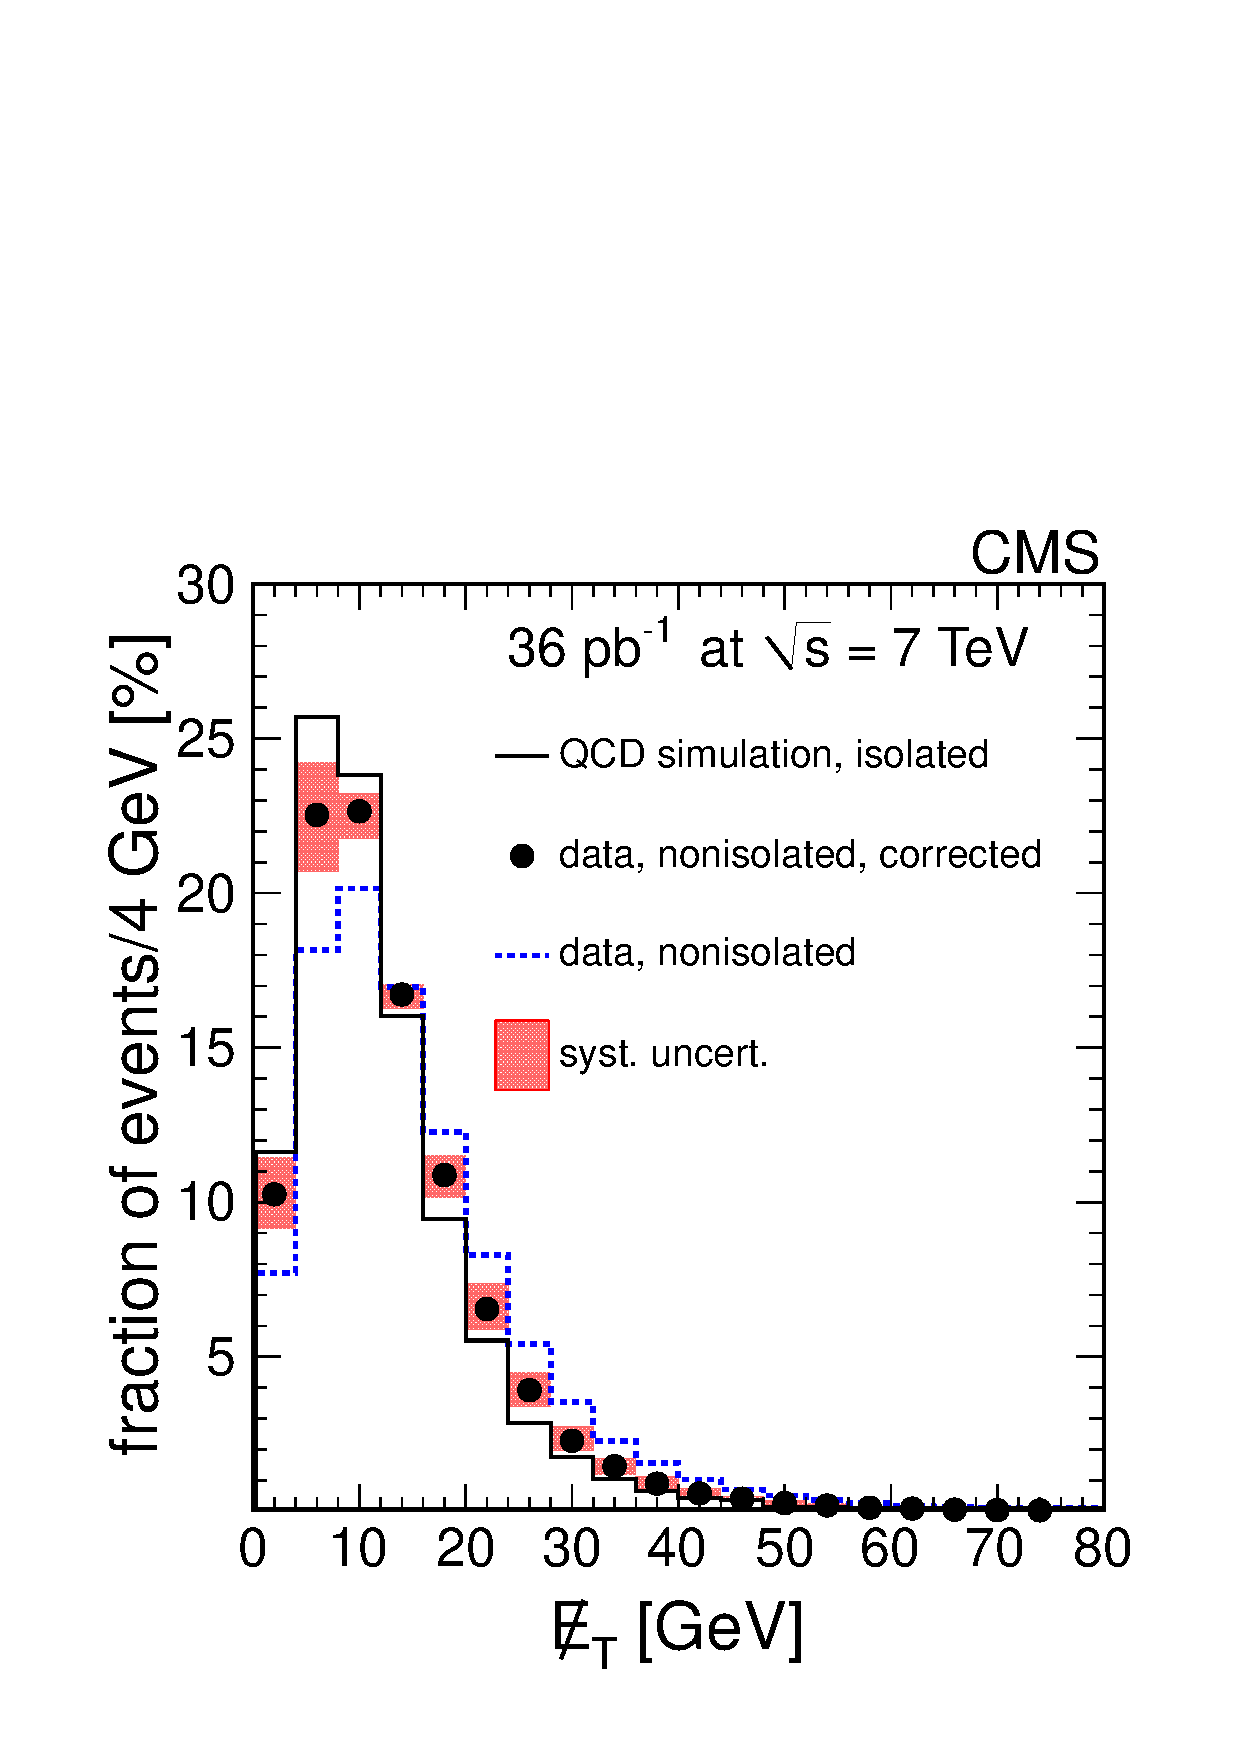
\includegraphics[width=7.5cm]{figs/qcd_template.pdf}
    \caption{
Distribution of the corrected $\MET$ for selected events
with a nonisolated muon in data (black points) superimposed
on the uncorrected $\MET$ distributions for data (blue dashed line) and
simulated QCD events (black, solid histogram, same as
the black, solid histogram in Fig.~\ref{figure:Wmunu_QCD}).
The shaded area represents the systematic uncertainty due to corrections with factors
$\alpha \pm \Delta \alpha$ for $\Delta \alpha = 0.08$.
    \label{figure:Wmunu_QCD_data}}
}
\end{figure}

The same positive correlation between $\MET$ and $\IRelComb$ is observed in the data
(blue squares in Fig.~\ref{figure:Wmunu_QCD}, right).
A correction $\MET^\prime = \MET/(1+\alpha\,\IRelComb)$, with $\alpha \approx 0.2$,
was applied.
The shapes obtained in data are shown in Fig.~\ref{figure:Wmunu_QCD_data} where
the uncorrected and corrected data shapes from events selected by inverting the isolation requirement, together with the
simulation expectation for events with an isolated muon, are shown.
The shaded area in Fig.~\ref{figure:Wmunu_QCD_data} is bounded by the two distributions, obtained using two extreme correction
parameters $\alpha \pm \Delta \alpha$, with $\Delta \alpha = 0.08$, as evaluated in simulations.
This area is taken as a systematic uncertainty on the QCD background shape.

Several parameterizations for the correction are considered,
but the impact on the corrected distribution and therefore on the final result is small.
Associated uncertainties on the cross section and ratios are evaluated as the differences between
the fit results obtained with the optimal $\alpha$ value and
two extreme cases, $\alpha \pm \Delta \alpha$.


The following signal yields are obtained: $140\,757 \pm 383$ for the inclusive sample,
$56\,666\pm240$ for the $\Wmmn$ sample, and $84\,091\pm291$ for the $\Wpmn$ sample.

The $\MET$ distributions are presented in
Fig.~\ref{figure:Wmunu_exp_fit} (full sample) and Fig.~\ref{figure:Wmn_PlusMinus}
 (samples selected by the muon charge) superimposed on the individual fitted
contributions of the W signal and the EWK and QCD backgrounds.
Figures~\ref{figure:Wmunu_exp_fit} and~\ref{figure:Wmn_PlusMinus}
show the $\MET$ distributions for data and fitted signal, plus background components.
 Figure~\ref{figure:Wmunu_exp_fit_mt}
% and~\ref{figure:Wmn_PlusMinus_mt}
shows the $\MT$ distributions for data and signal, plus background components, fitted
from the $\MET$ spectra.

% The fitted W parameters are summarized in Tables~\ref{table:Wmunu_tot_xs}
% for the two choices of fit parameters. The error shown is only statistical.
 \begin{figure}[!ht] {\centering
   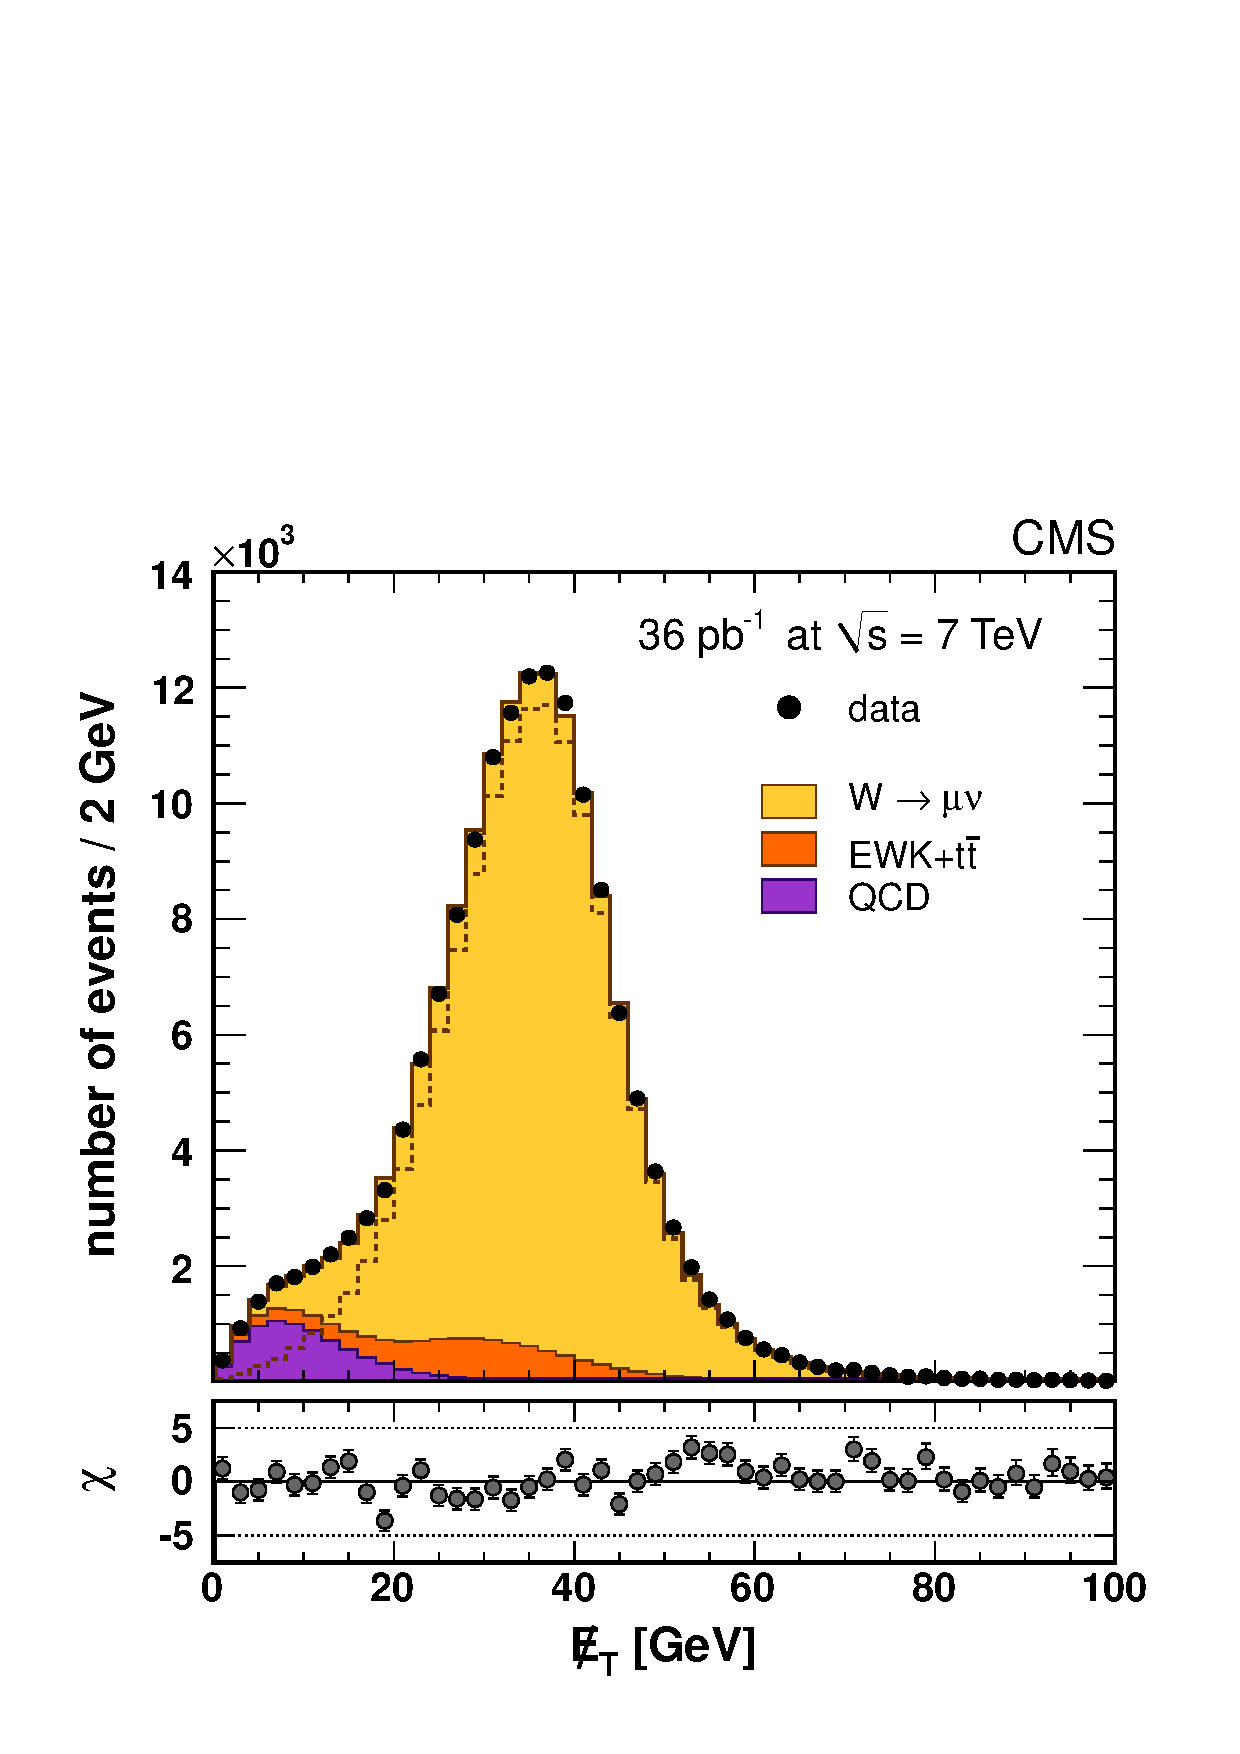
\includegraphics[width=7cm]{figs/Wmn_MET.pdf}
   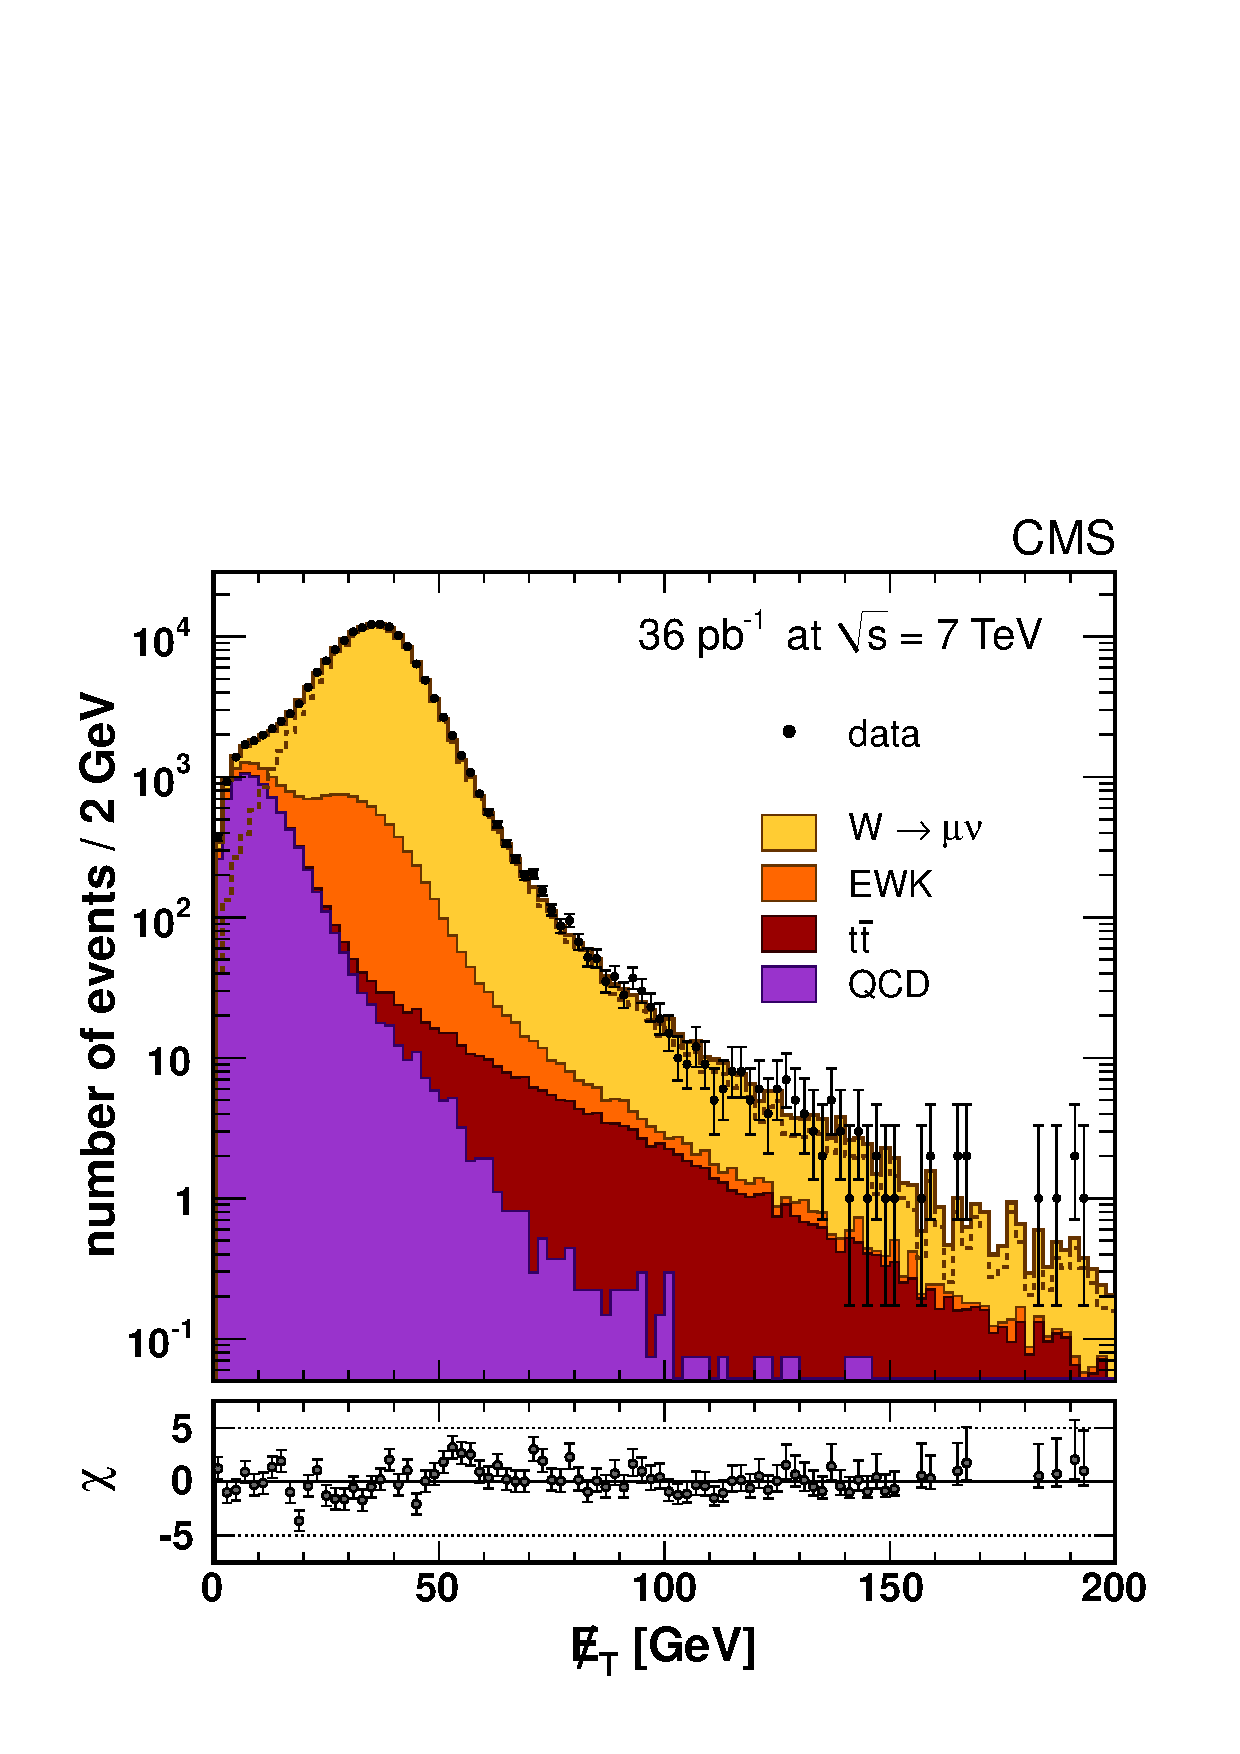
\includegraphics[width=7cm]{figs/Wmn_MET_log.pdf}
     \caption{
The $\MET$ distribution for the selected $\Wmn$ candidates on
a linear scale (left) and on a logarithmic scale (right).
The points with the error bars represent the data. Superimposed are the
contributions obtained with the fit
for QCD background (violet, dark histogram), all other backgrounds
(orange, medium histogram), and signal plus  background (yellow, light histogram).
The black dashed line is the fitted signal contribution.
     \label{figure:Wmunu_exp_fit}}
}
 \end{figure}

\begin{figure}[!ht] {\centering
   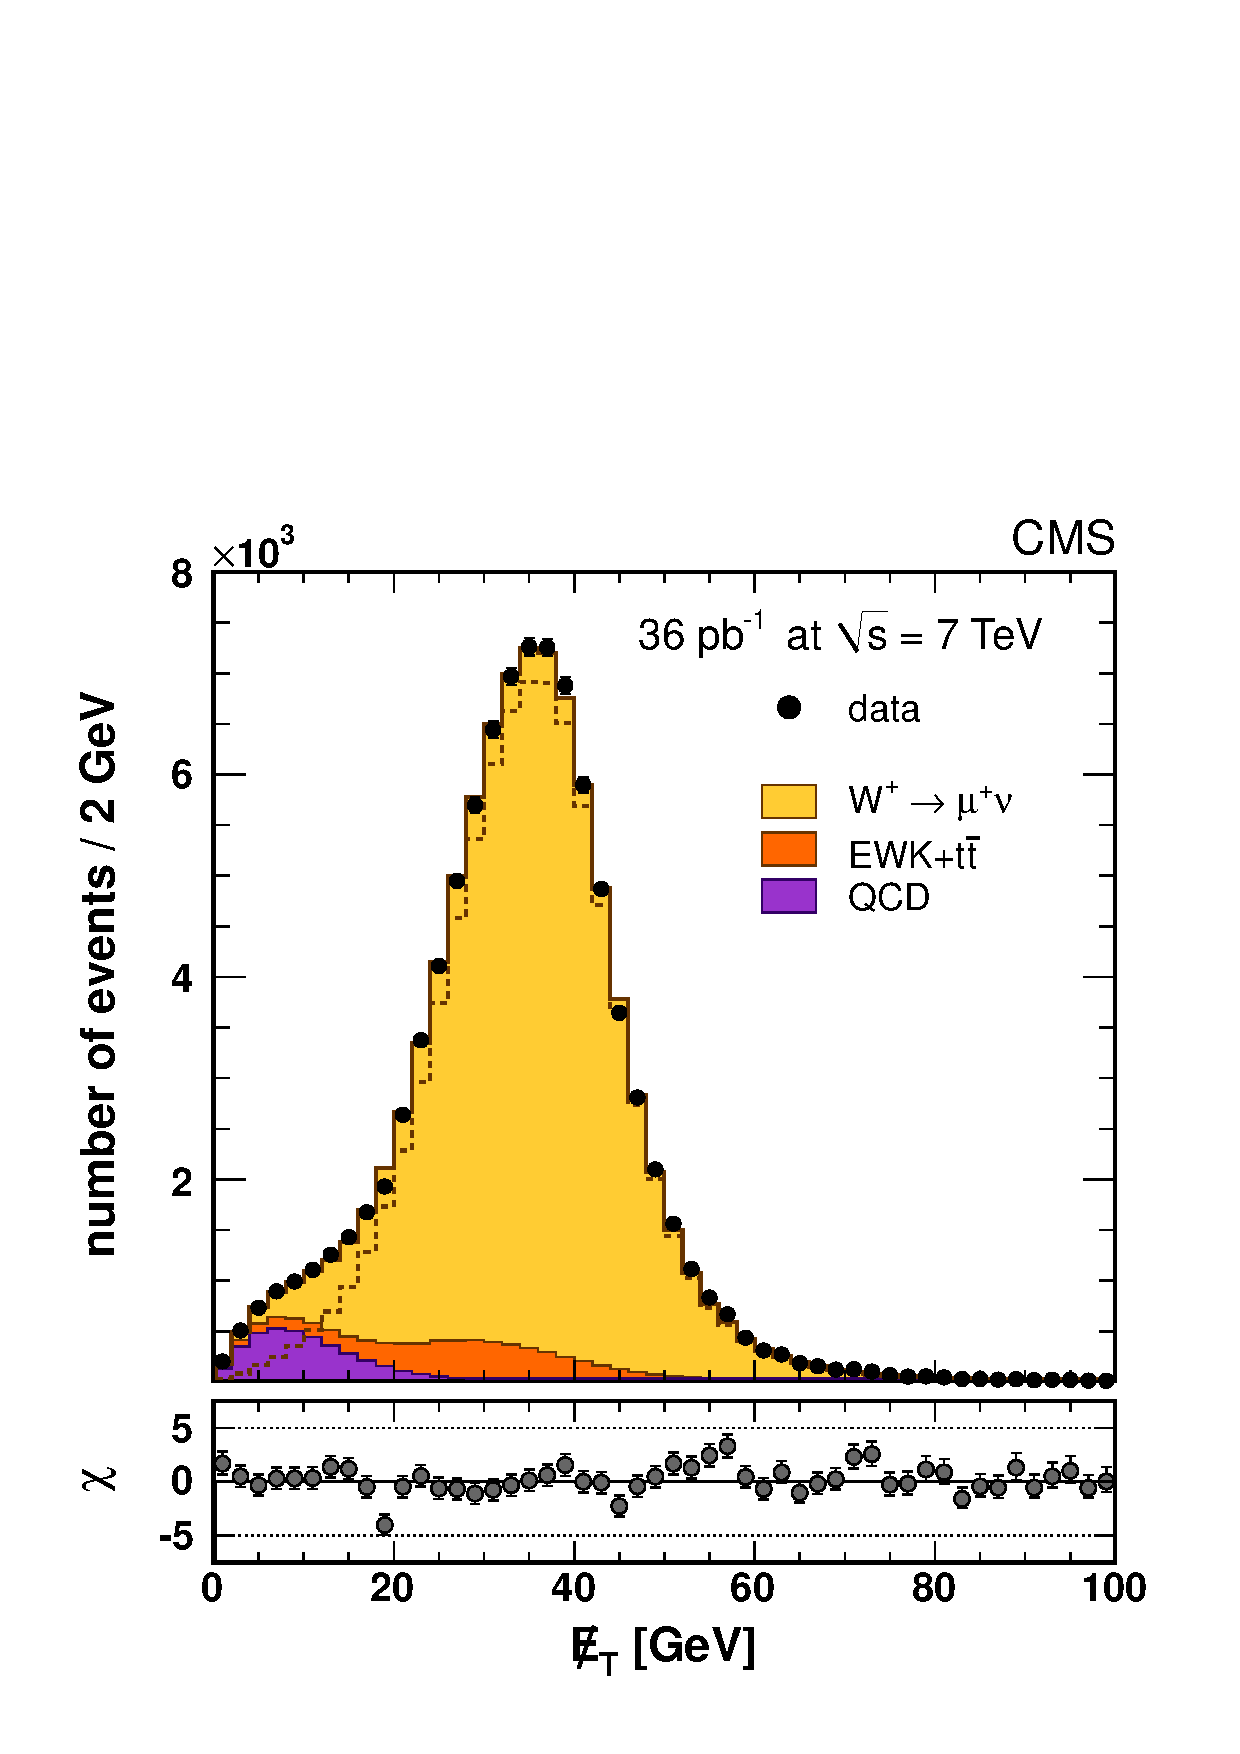
\includegraphics[width=7cm]{figs/Wmn_MET_plus.pdf}
   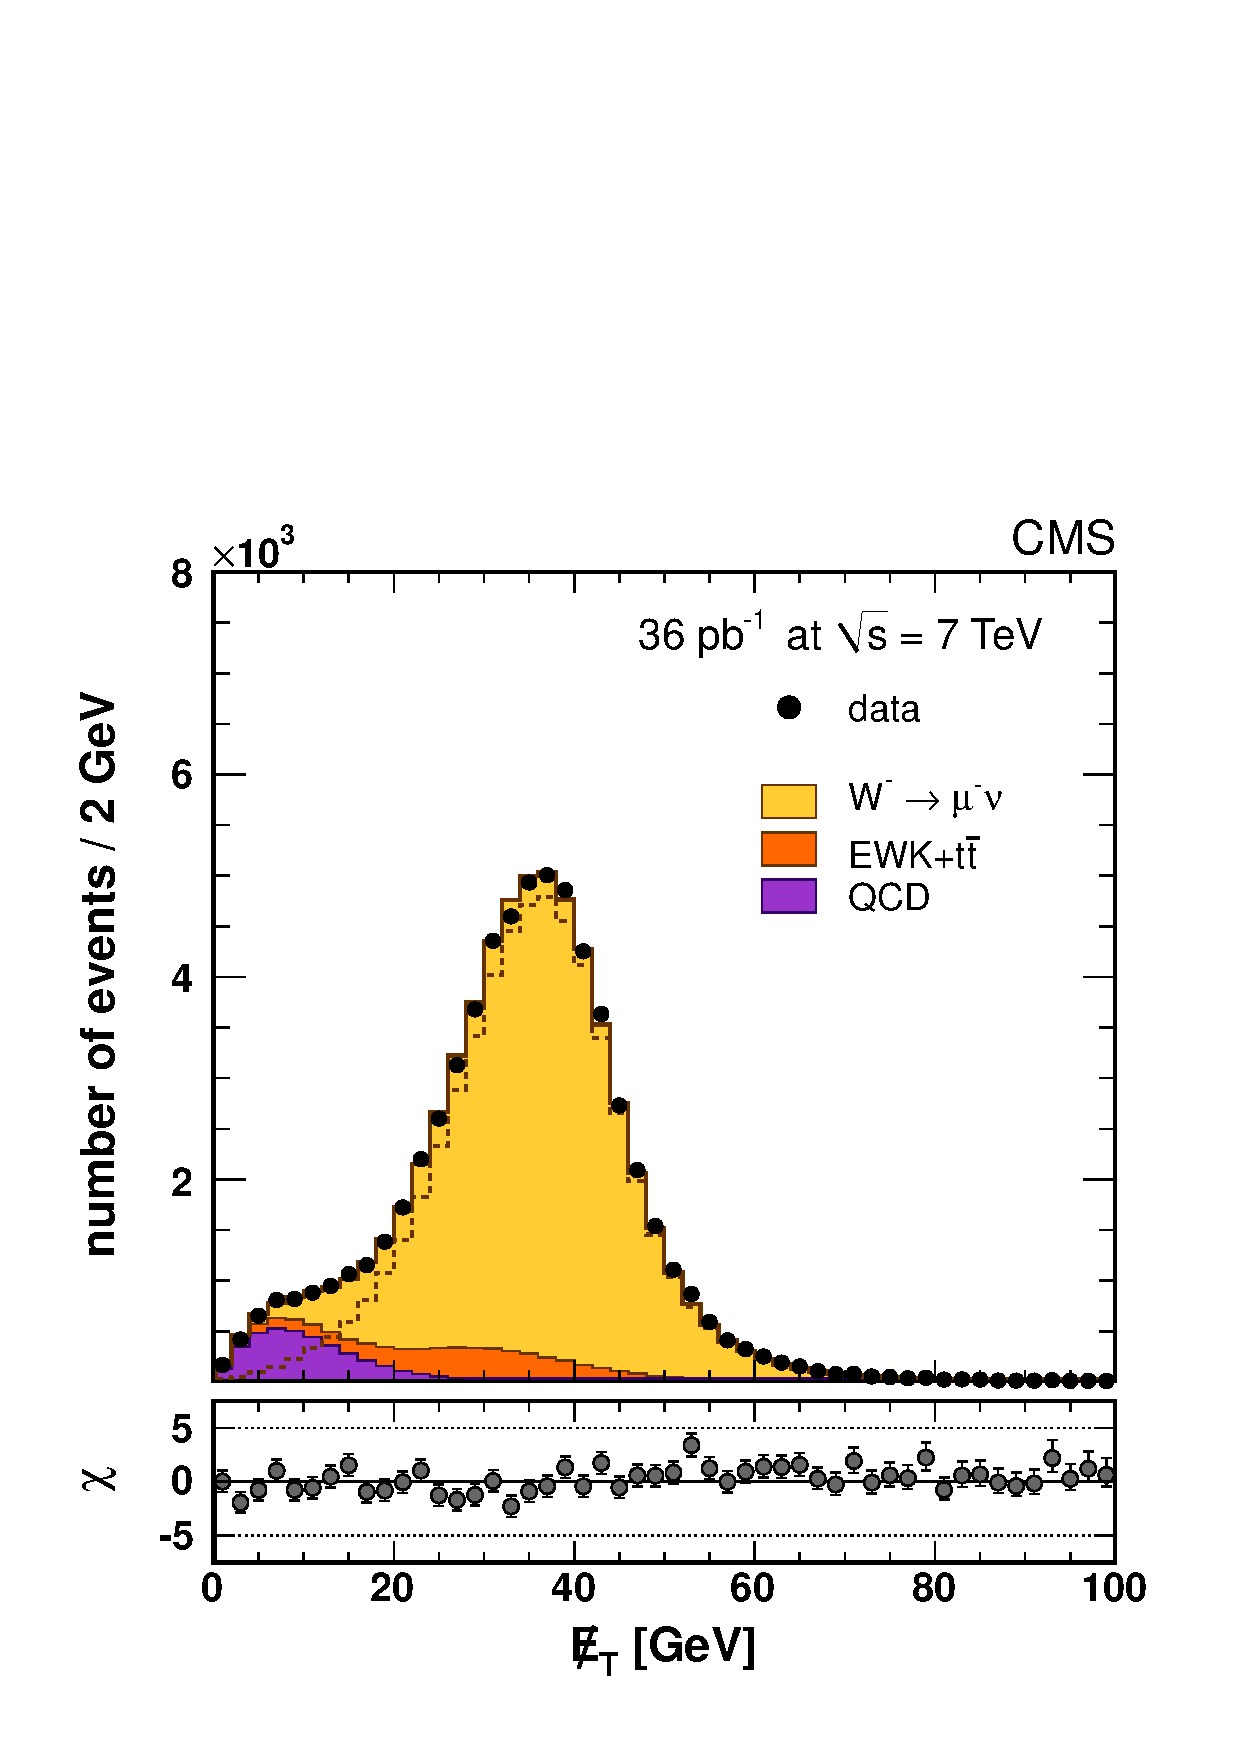
\includegraphics[width=7cm]{figs/Wmn_MET_minus.pdf}
    \caption{
The $\MET$ distributions for the selected W$^+$ (left) and W$^-$ (right) candidates.
The points with the error bars represent the data. Superimposed are the contributions
obtained with the fit for QCD background (violet, dark histogram), all other backgrounds
(orange, medium histogram), and signal plus background (yellow, light histogram).
The black dashed line is the fitted signal contribution.
    \label{figure:Wmn_PlusMinus}}
}
\end{figure}

 \begin{figure}[!ht] {\centering
   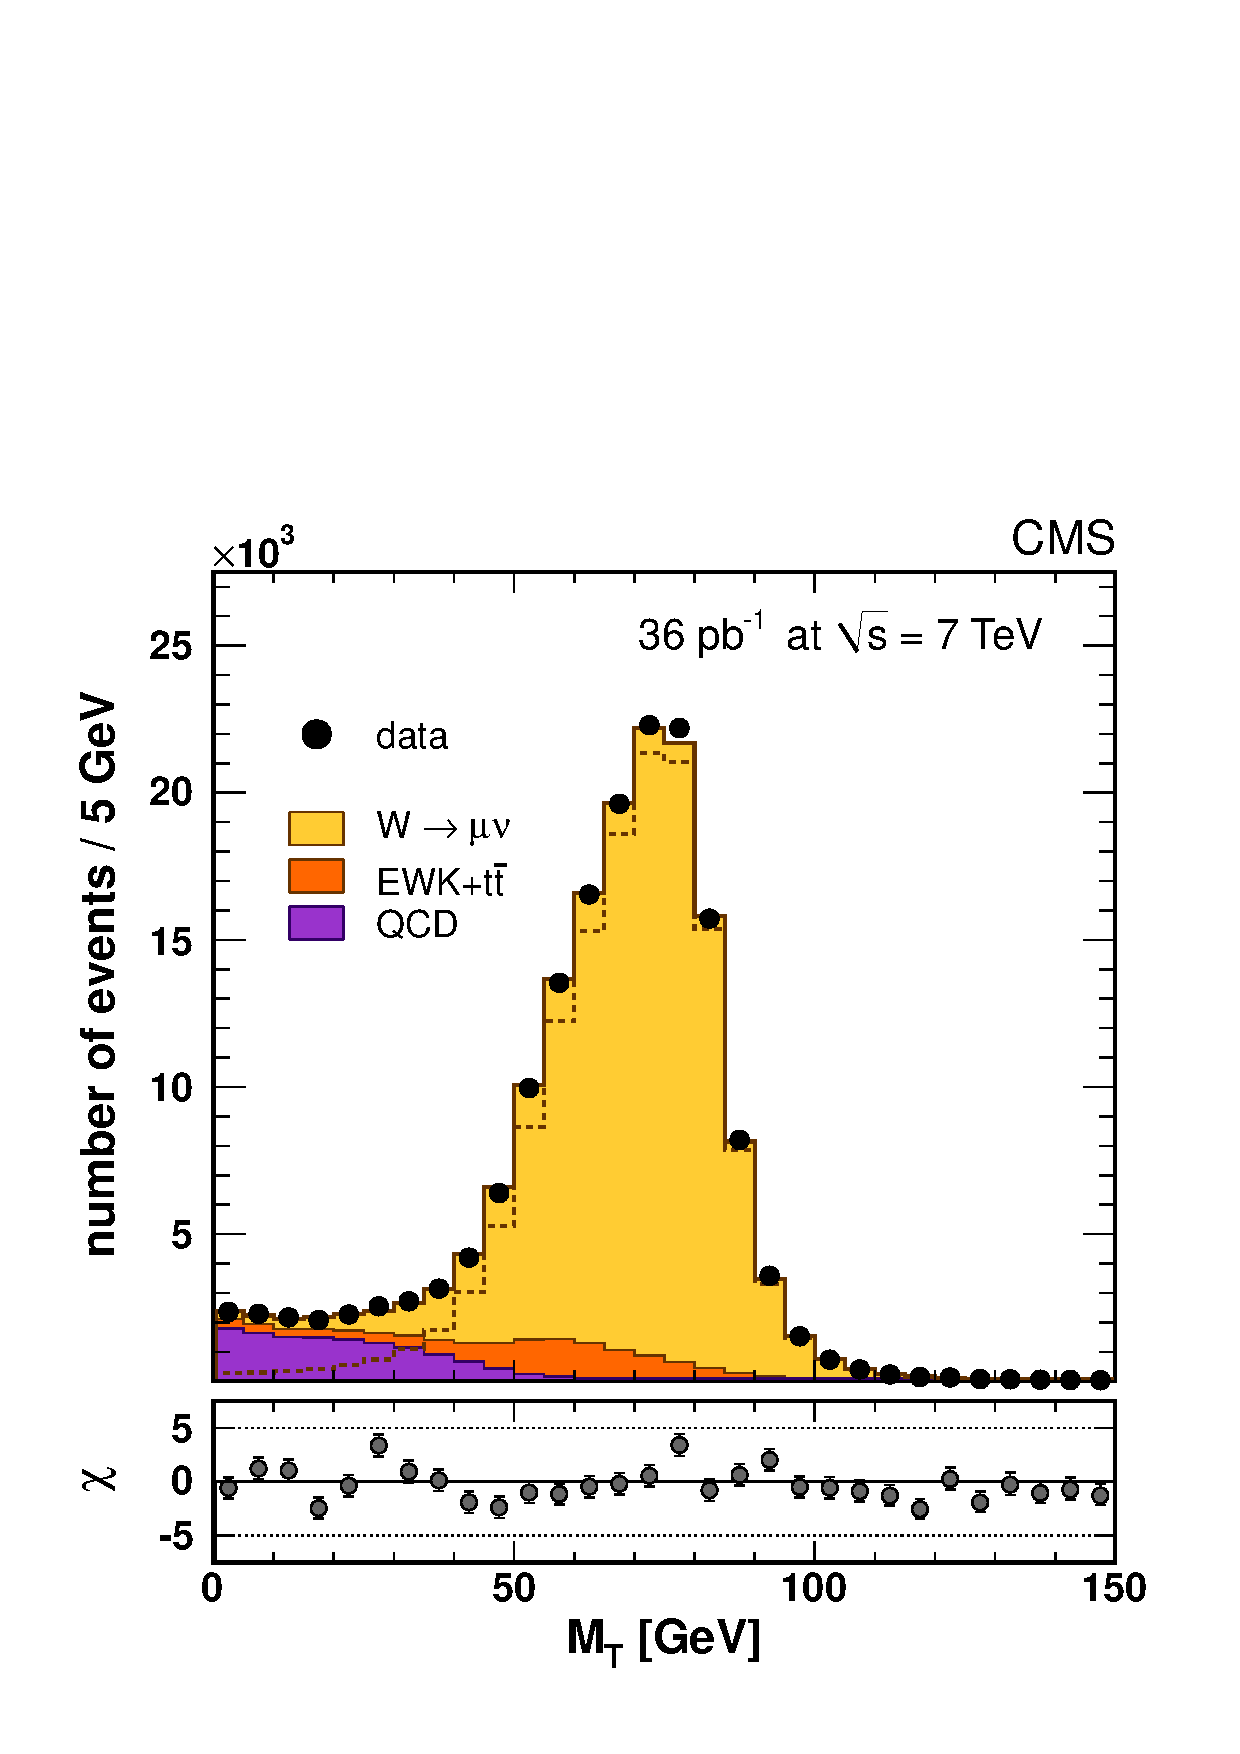
\includegraphics[width=7cm]{figs/Wmn_MT.pdf}
   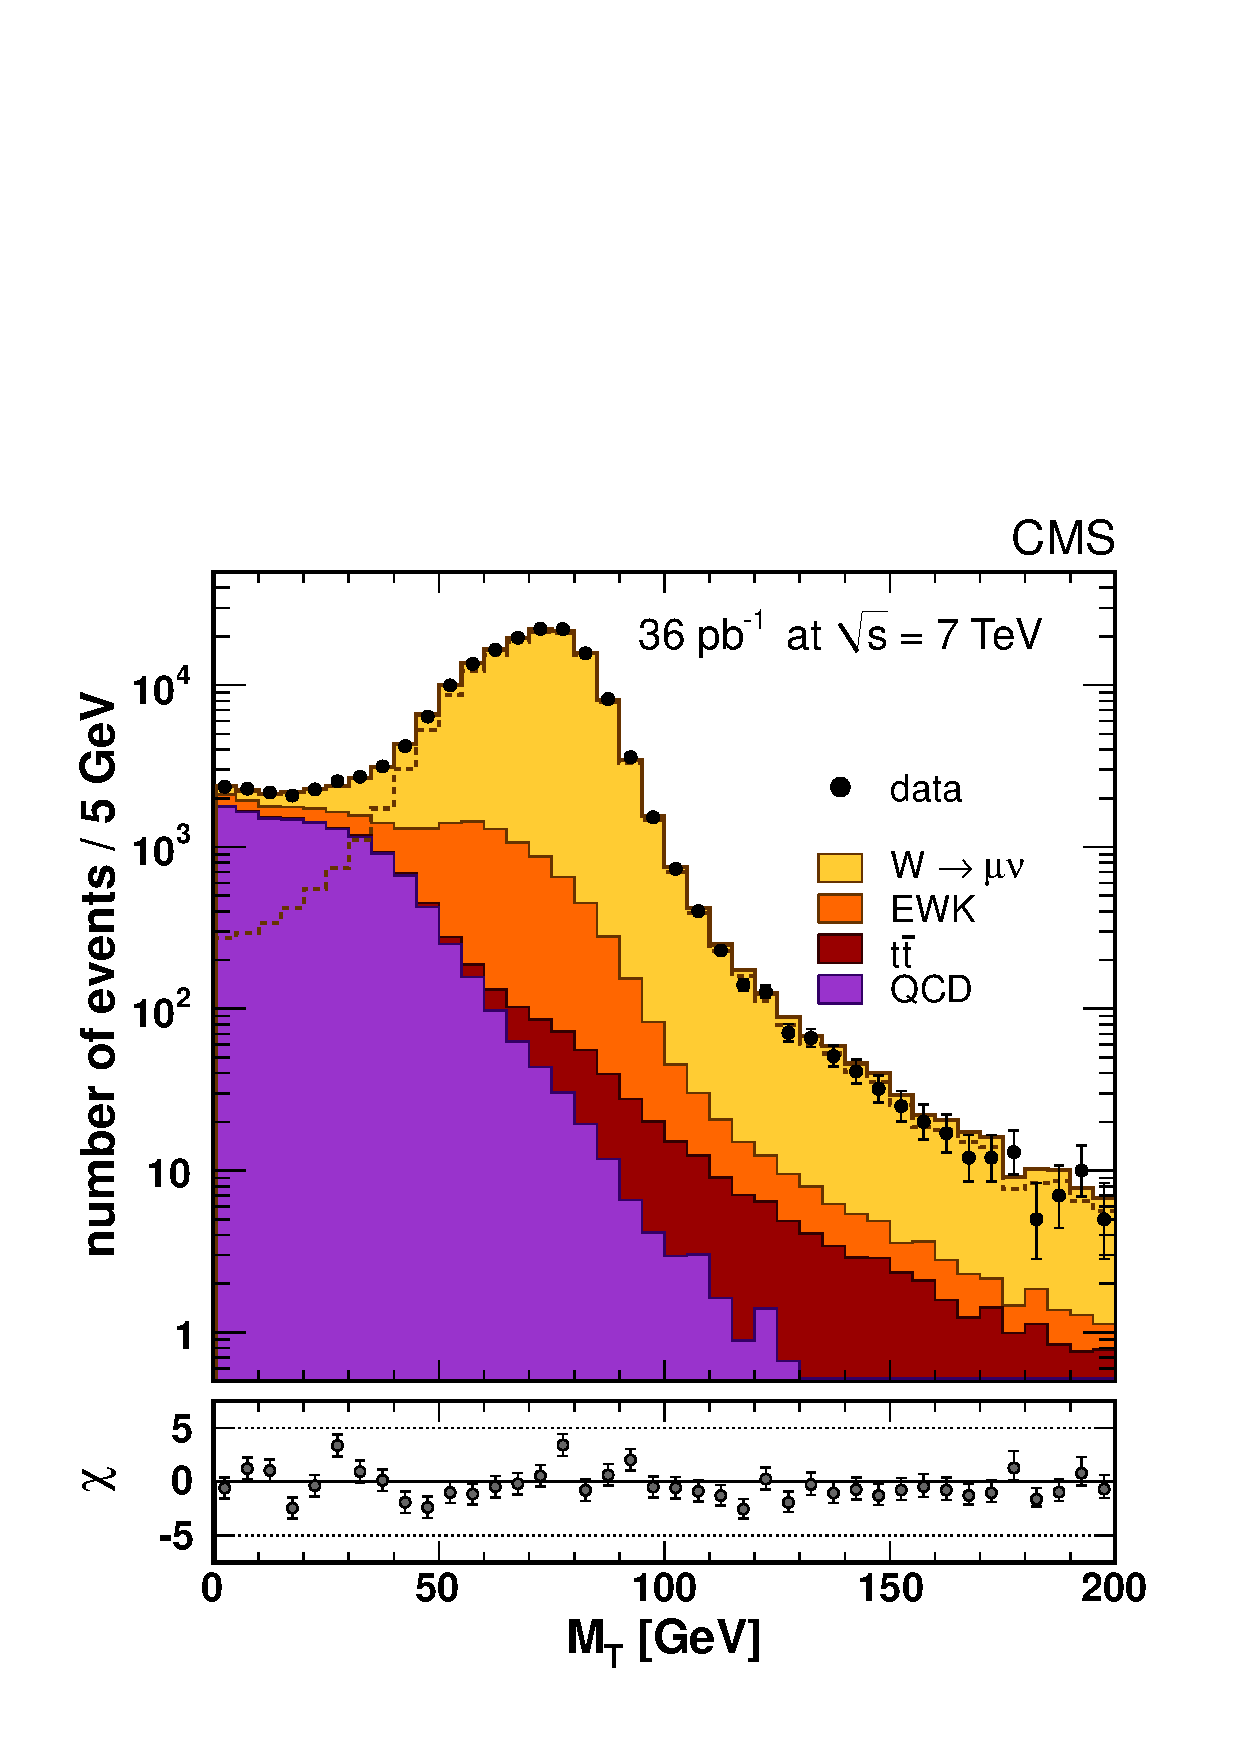
\includegraphics[width=7cm]{figs/Wmn_MT_log.pdf}
     \caption{
The $\MT$ distribution for the selected $\Wmn$ candidates on
a linear scale (left) and on a logarithmic scale (right).
The points with the error bars represent the data. Superimposed are the
contributions obtained with the fit
for QCD background (violet, dark histogram), all other backgrounds
(orange, medium histogram), and signal plus background (yellow, light histogram).
The black dashed line is the fitted signal contribution.
     \label{figure:Wmunu_exp_fit_mt}}
}
 \end{figure}



\section{\texorpdfstring{The $\Zll$ Signal Extraction}{The Z-> ll Signal Extraction}}
\label{sec:ZsignalExtraction}

The $\Zll$ yield can be obtained by counting the
number of selected candidates after subtracting the residual background.
The $\Zll$ yield and lepton efficiencies are also determined using a simultaneous fit
to the invariant mass spectra of multiple dilepton categories.
The simultaneous fit deals correctly with correlations
in determining the lepton efficiencies and the $\Zo$ yield
from the same sample.
The Z yield extracted in this way does not need to be corrected for efficiency effects
in order to determine the cross section, and
the statistical uncertainty on the $\Zo$ yield absorbs the uncertainties
on the determination of lepton efficiencies that would be propagated as systematic
uncertainties in the counting analysis.
Both methods were performed for the $\Zee$ analysis, while only
the simultaneous fit was used for the $\Zmm$ analysis
after taking into account the results from the previous studies~\cite{WZCMS:2010}.
%at lower luminosity which disfavour the use of the counting analysis.

\subsection{EWK and QCD Backgrounds}
\label{sec:bkgZll}

For the $\Zee$ analysis the background contributions from EWK processes $\Ztt$, $\ttbar$,
and diboson production are estimated from the yields of events selected in NLO MC samples
normalized to the NNLO cross sections and scaled to the considered integrated luminosity.
They amount to \ZEEEWKBKG events, where the uncertainty combines the NNLO
and luminosity uncertainties. Data are used to estimate the background
originating from W+jets, $\gamma$+jets, and QCD multijet events where the
selected electrons come from misidentified jets or photons
(referred to as 'QCD background').
This background contribution is estimated using the distribution
of the relative track isolation, $\ITRK/\Et$,
and amounts to $4.9 \pm 8.4\, \textrm{(stat.)} \pm 8.4\, \textrm{(syst.)}$ events.
As a cross-check, the ``same-sign/opposite-sign'' method was used,
which is based on the signs of the charges of the two electron candidates, the measured
charge misidentification for electrons that pass the nominal selection criteria, and the
hypothesis that the QCD background is charge-symmetric.
The QCD background estimate with this method is $59 \pm 17
\textrm{(stat.)} \pm 160\, \textrm{(syst.)}$ events.
The two methods are consistent with the presence of negligible QCD background in our sample.

Backgrounds in the $\Zmm$ analysis containing two isolated global muons
have been estimated with simulations to be very small.
This category of dimuon events is defined as the ``golden'' category.
The simulation prediction of the smallness of the $\ttbar$ and QCD backgrounds was validated with data.
First, the selected dimuon sample was enriched with $\ttbar$ events by applying
a requirement on $\MET$, because of the presence of neutrinos in $\ttbar$ events,
and an agreement between data and the simulation prediction was found
with the dimuon invariant mass requirement inverted,
where the residual Z signal is negligible.
The QCD component has been checked using the same-sign dimuon events and dimuon events with
both muons failing the isolation requirement, and was found to be in agreement with the simulation predictions.
The conclusion from the maximum amount of measured data-simulation discrepancy
was that the uncertainty in the residual background subtraction
has a negligible effect on the $\Zmm$ measured yield.
The backgrounds to the $\Zmm$ categories having one global and one looser muon
are significantly larger than in the golden category.
Simulation estimates in this case are not used for such backgrounds and
fits to the dimuon invariant mass
distributions are performed including parameterized background components, as
described in Section~\ref{sec:Zmumu}.

Backgrounds estimates in the $\Zee$ and $\Zmm$ analyses are summarized in Table~\ref{tab:ZllBG}.
%--------------------------------------------------
\begin{table} %
\begin{center}
\caption[.]{\label{tab:ZllBG}
Estimated background-to-signal ratios in the $\Zee$ and $\Zmm$ (only for candidates
in the golden category) channels.
The QCD background for the $\Zee$ channel has been estimated with data,
while all other estimates are based on MC simulations, and their corresponding uncertainties
are statistical only.}
\begin{tabular}{|l|c|c|}
\hline
Processes & $\Zee$ sel. & $\Zmm$ sel. \\
\hline\hline
Diboson production   & $(0.157\pm 0.001)\%$ & $(0.158\pm 0.001)\%$ \\
$\ttbar$             & $(0.117\pm 0.008)\%$ & $(0.141\pm 0.014)\%$ \\
$\Ztt$               & $(0.080\pm 0.006)\%$ & $(0.124\pm 0.005)\%$ \\
W+jets               & $(0.010\pm 0.002)\%$ & $(0.008\pm 0.002)\%$ \\
\hline
Total EWK plus $\ttbar$  & $(0.365\pm 0.010)\%$ & $(0.430\pm 0.015)\%$ \\
\hline
QCD            & $(0.06\pm 0.14)\%$ &  $(0.013\pm 0.001)\%$ \\
\hline
Total background                & $(0.42\pm 0.14)\%$ & $(0.444\pm 0.015)\%$ \\
\hline
\end{tabular}
\end{center}
\end{table}



%--------------------------------------------------


\subsection{\texorpdfstring{The $\Zee$ Signal Extraction}{The Z->ee Signal Extraction}}

In the following sections the use of a pure $\Zee$ sample
for the determination of the residual energy-scale and resolution corrections is first discussed.
Then the signal extraction with the counting analysis and the
simultaneous fit methods are presented.

\subsubsection{Electron Energy Scale}
\label{sec:e-escale}

The lead tungstate crystals of the ECAL are subject to transparency loss
during irradiation, followed by recovery in periods with no
irradiation. The magnitude of the changes to the energy response is
dependent on instantaneous luminosity and was, at the end of the 2010
data taking period, up to 1$\%$ in the barrel region, and 4$\%$ or more in
parts of the endcap. The changes are monitored continuously by injecting
laser light and recording the response. The corrections derived from
this monitoring are validated by studying the variation of the $\pi^0$ mass
peak as a function of time for different regions of the ECAL (using $\pi^0$ data
collected in a special calibration stream), and by studying the overall $\Zee$ mass peak and width.
%The correction
%calculations are still being developed and commissioned, and the
%corrections provided for the current reconstruction do not yet achieve
%the target precision. However, the validation and testing show that the
%residual variation of the energy scale with time, using these
%corrections, is less than 0.3$\%$ in the barrel and less than 1$\%$ in the
%endcap.
%
% from Isabel
%
With the current corrections, residual variations of the energy scale with time are
at the level of 0.3\% in the barrel and less than 1\% in the endcaps.


\par
%
% Isabel suggests to rewrite this section
%
%
The remaining mean scale correction factors to be applied to the data and the
resolution corrections (smearing) to be applied to the simulated sample
are estimated from $\Zee$ events. Invariant mass distributions for electrons
in several $\eta$ bins in the EB and EE are derived
from simulations and compared to data. A simultaneous fit of a Breit--Wigner convolved with a
Crystal-Ball function to each $\Zee$ mass distribution is performed  in order
to determine the energy scale correction factors for the data and the resolution
smearing corrections for the simulated samples. The energy scale correction
factors are below 1$\%$ while the resolution smearing corrections are below 1$\%$
everywhere, with the exception of the transition region between the EB and the EE,
where they reach 2$\%$.
Those corrections are propagated in the analysis and proper systematic uncertainties
for the cross section measurements are estimated as discussed in Section~\ref{subsec:ELEsystematics}.
%
%
% The remaining mean scale correction factors to be applied to the data and the
% resolution correction (smearing) to be applied to the simulated sample
% are estimated as follows.
% The $\Zee$ events are divided into categories that correspond to all possible
% combinations of four $\eta$ bins in the EB and two $\eta$ bins in the EE.
% An invariant mass distribution is derived from simulations in each category.
% A simultaneous fit of a Breit-Wigner convolved with a Crystal-Ball function
% to the $\Zee$ mass distribution is performed in each of the $\eta$ bins, in order
% to determine the energy scale correction factors for the data and the resolution
% smearing correction factors for the simulated samples.
% The energy scale correction factors for the data and the resolution smearing correction
% factors for the simulated samples for the tight selection are reported
% in Table~\ref{tab:EnergyScaleResolution}.
%
% \begin{table}[ht] %
%   \begin{center}
%   \caption{ Energy scale correction factors for the data and
% resolution smearing correction factors for the simulated samples
% to be applied per electron for various $\eta$ bins.
%   \label{tab:EnergyScaleResolution}}
%   \begin{tabular}{|l|c|c|}
%     \hline
%     Region  & Energy scale & Resolution Correction (smearing) [GeV] \\
%     \hline\hline
% $0.0<|\eta|<0.4$ & $0.9940\pm0.0010$ & $0.29\pm0.20$ \\
% $0.4<|\eta|<0.8$ & $0.9958\pm0.0011$ & $0.30\pm0.23$ \\
% $0.8<|\eta|<1.2$ & $0.9992\pm0.0012$ & $0.37\pm0.22$ \\
% $1.2<|\eta|<1.5$ & $1.0079\pm0.0020$ & $1.07\pm0.19$ \\
% $1.5<|\eta|<2.0$ & $0.9955\pm0.0019$ & $1.04\pm0.22$ \\
% $2.0<|\eta|<2.5$ & $1.0003\pm0.0013$ & $0.18\pm0.15$ \\
%     \hline
%     \end{tabular}
%   \end{center}
% \end{table}

\par
%
% This probably deserves to be put in a separate section instead of "Electron energy Scale"
% (Luca)
%
\subsubsection{Counting Analysis}
After energy scale corrections, applied to electron ECAL clusters before
any threshold requirement, 10 fewer events ($-0.12\%$) were selected compared to the number of selected
events before the application of the energy scale corrections.
This brings the final $\Zee$ sample to $\ZEESAMPLEN$ and, after
background subtraction, the $\Zo$ yield is $\ZEEYIELD$ events.
This yield is used for the cross section estimation.
%
% If this is not the result of the fit but just the counting
%


\par
The dielectron invariant mass spectra for the selected sample
with the tight selection before and after the application of the corrections are
shown in Fig.~\ref{fig:Zee} along with the predicted distributions.
The data and simulation distributions are normalized to account for the difference in selection
efficiency.

%%%%%
\begin{figure}
  \begin{center}
   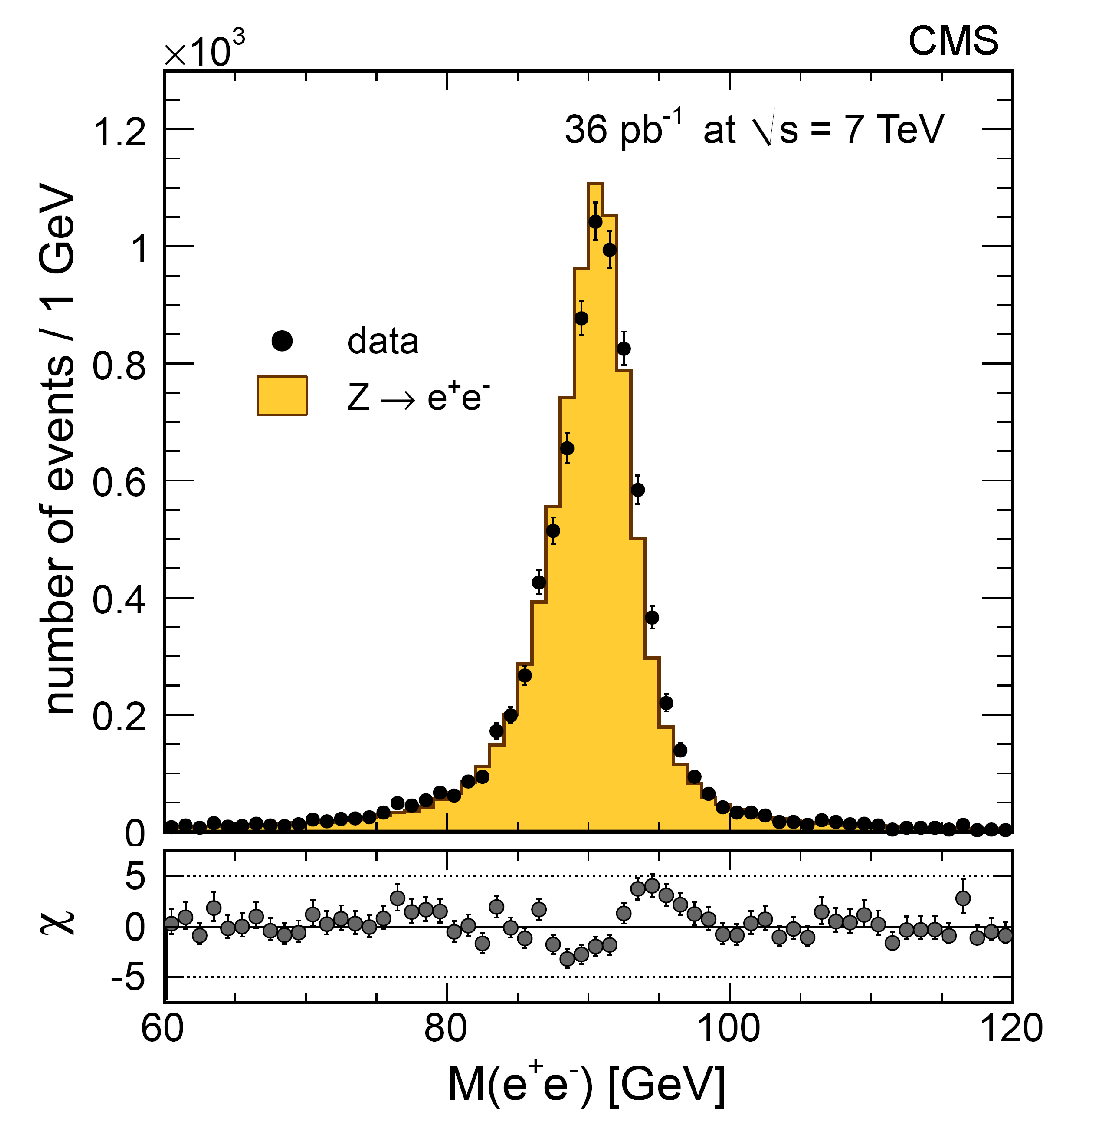
\includegraphics[width=0.48\textwidth]{figs/Zee_mass_Linear.pdf}
   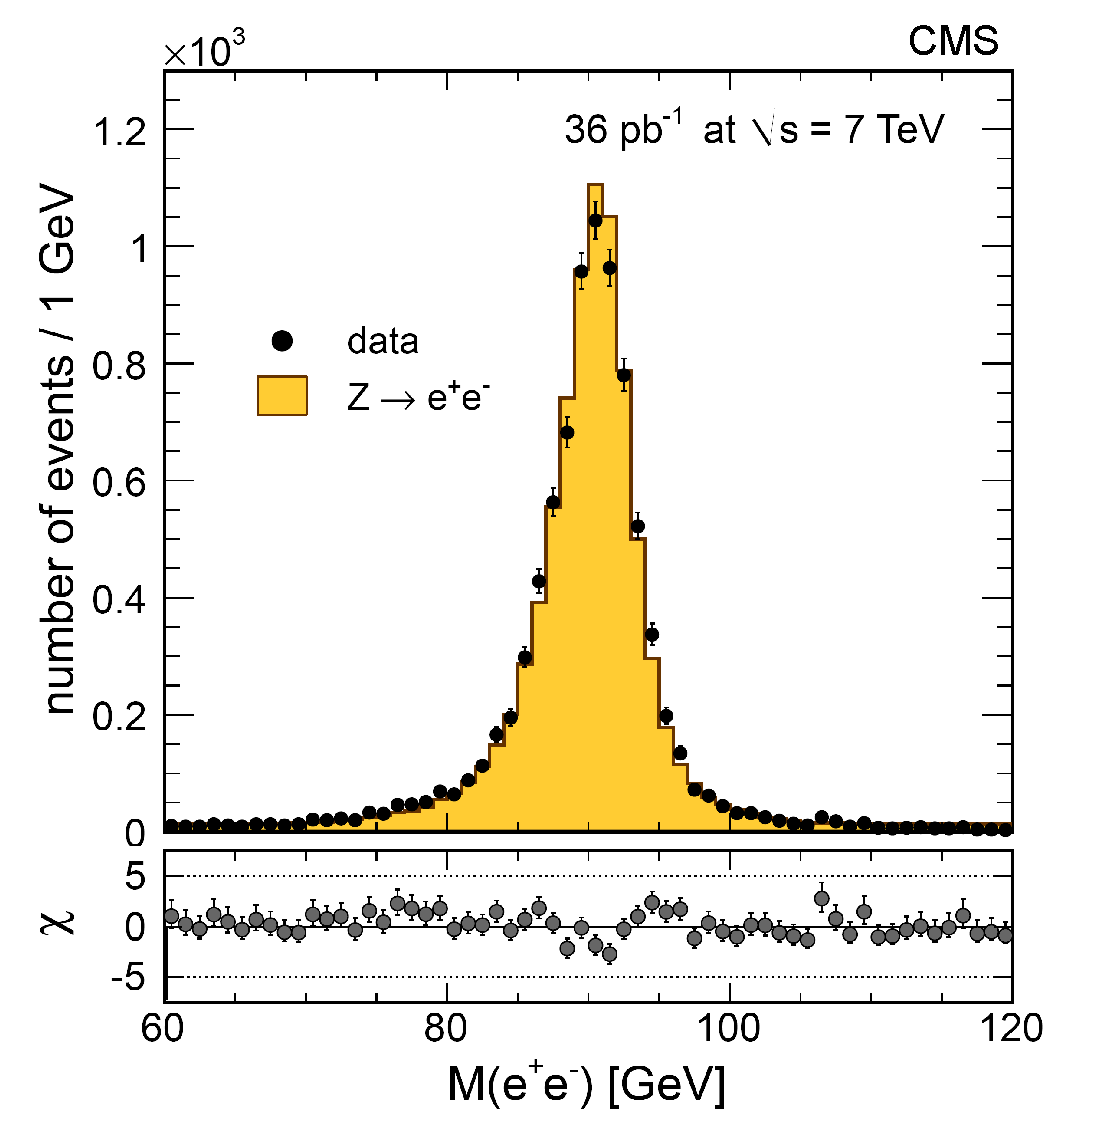
\includegraphics[width=0.48\textwidth]{figs/Zee_mass_Linear_corrected.pdf}
   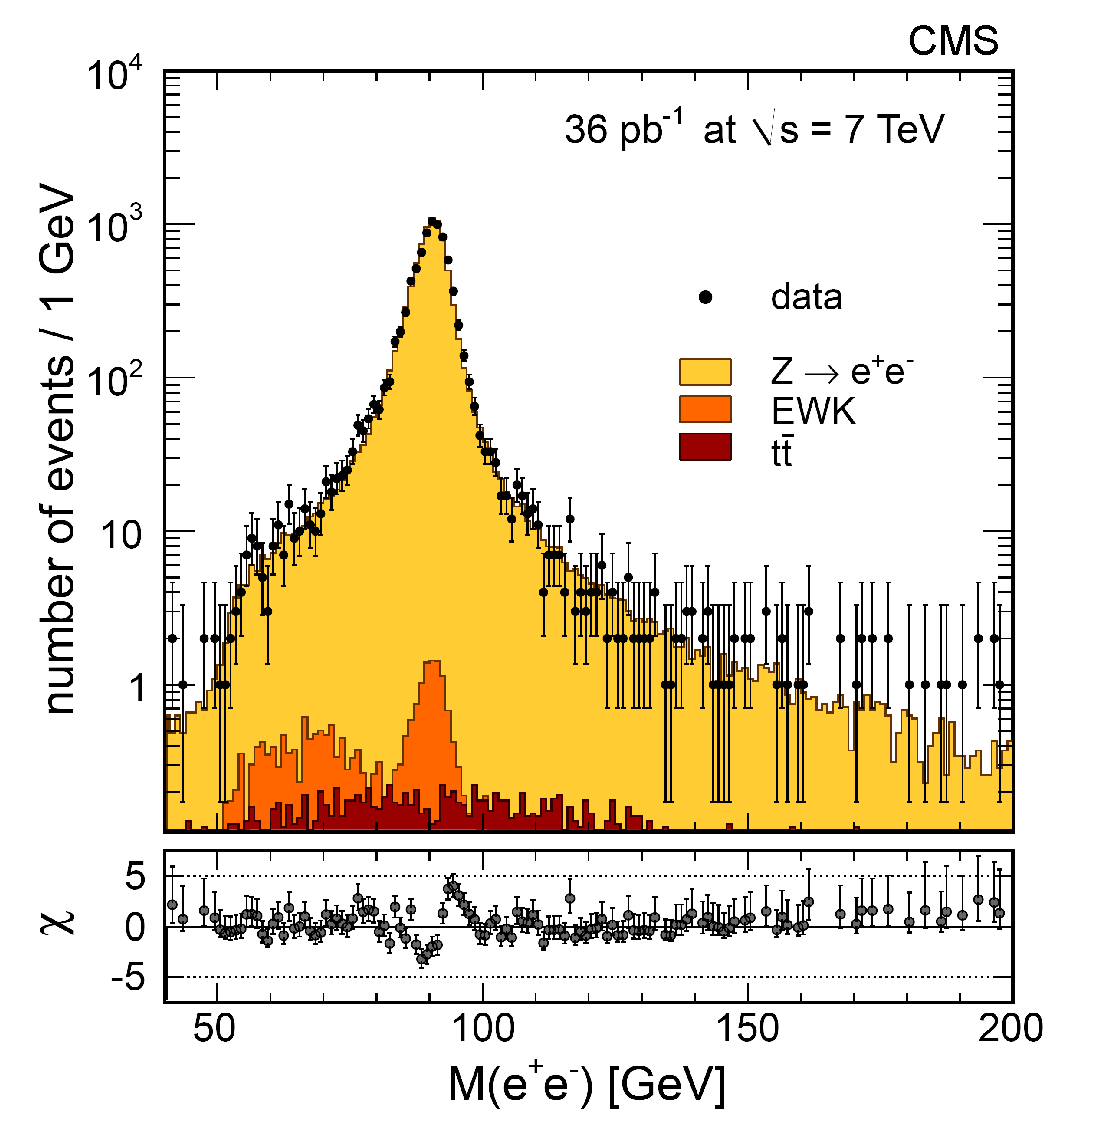
\includegraphics[width=0.48\textwidth]{figs/Zee_mass_Logarithmic.pdf}
   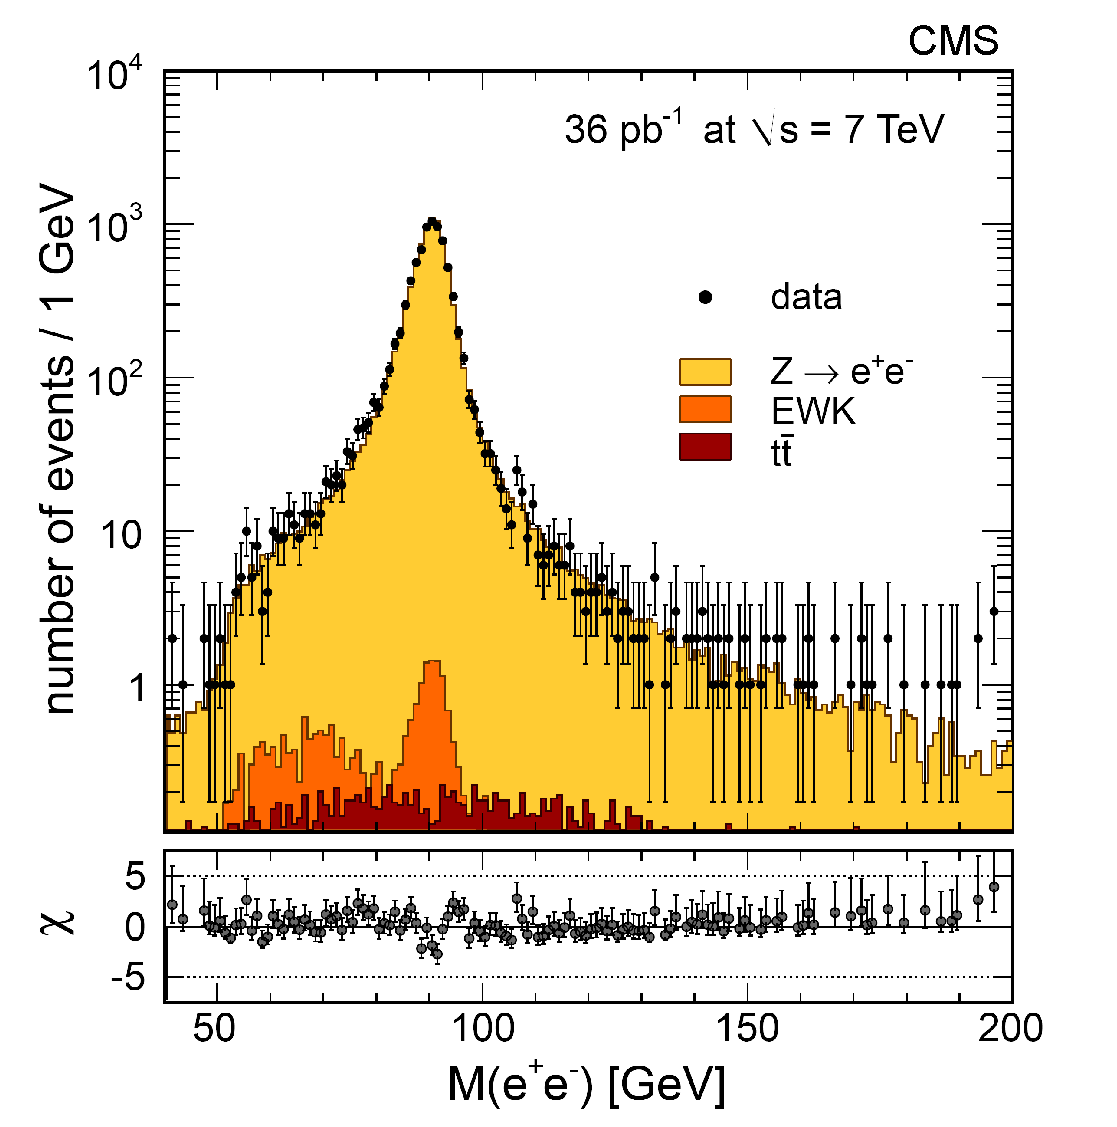
\includegraphics[width=0.48\textwidth]{figs/Zee_mass_Logarithmic_corrected.pdf}
   \caption{ \label{fig:Zee}
Distributions of the dielectron invariant mass for the selected $\Zee$ candidates on
a linear scale (top) and on a logarithmic scale (bottom) before (left)
and after (right) applying energy-scale correction factors.
The points with the error bars represent the data.
Superimposed are the expected distributions from simulations, normalized
to an integrated luminosity of $36$~pb$^{-1}$. The expected distributions are
the Z signal (yellow, light histogram), other EWK processes (orange, medium histogram),
and $\ttbar$ background (red, dark histogram).
Backgrounds are negligible and cannot be seen on the linear-scale plots.
}
  \end{center}
\end{figure}
%%%%%


\subsubsection{Simultaneous Fit}

The $\Zo$ event yield and the electron efficiencies can be extracted from
a simultaneous fit. Two categories of events are
considered: events where both electrons satisfy
the tight selection with $\Et>25\GeV$, and events that consist of
one electron with $\Et>25\GeV$ that passes the tight selection, and one
ECAL cluster with $\Et>25\GeV$ that fails
the selection, either at the reconstruction or electron identification level.

In each category, a signal-plus-background function is fitted to the observed mass spectrum.
The signal shape is taken from signal samples simulated with POWHEG at the NLO generator level,
and is convolved with a Crystal-Ball function modified to include an extra
Gaussian on the high end tail with floating mean and width.
In the first category, the nearly vanishing background is fixed to the
value reported in Table~\ref{tab:ZllBG}. In the second
category of events, the background is modeled by an exponential distribution.

%Fig.~\ref{fig:Zmass_TT_TF} shows the fit to the Tag-Tag events (left plot) and to
%Tag-Fail events (right plot).
The estimated cross section is $988 \pm 10\, \mathrm{(stat.)} \pm 4\mathrm{(syst.)}\,\mathrm{pb}$.
The cross section is in good agreement with the counting analysis estimate of
 $992 \pm 11\, \mathrm{(stat.)}\,\mathrm{pb}$, considering only the statistical uncertainty.
Both techniques give equivalent results. The counting analysis estimate is used for the
cross section measurement in the $\Zee$ channel.

%\begin{figure}
%  \begin{center}
%   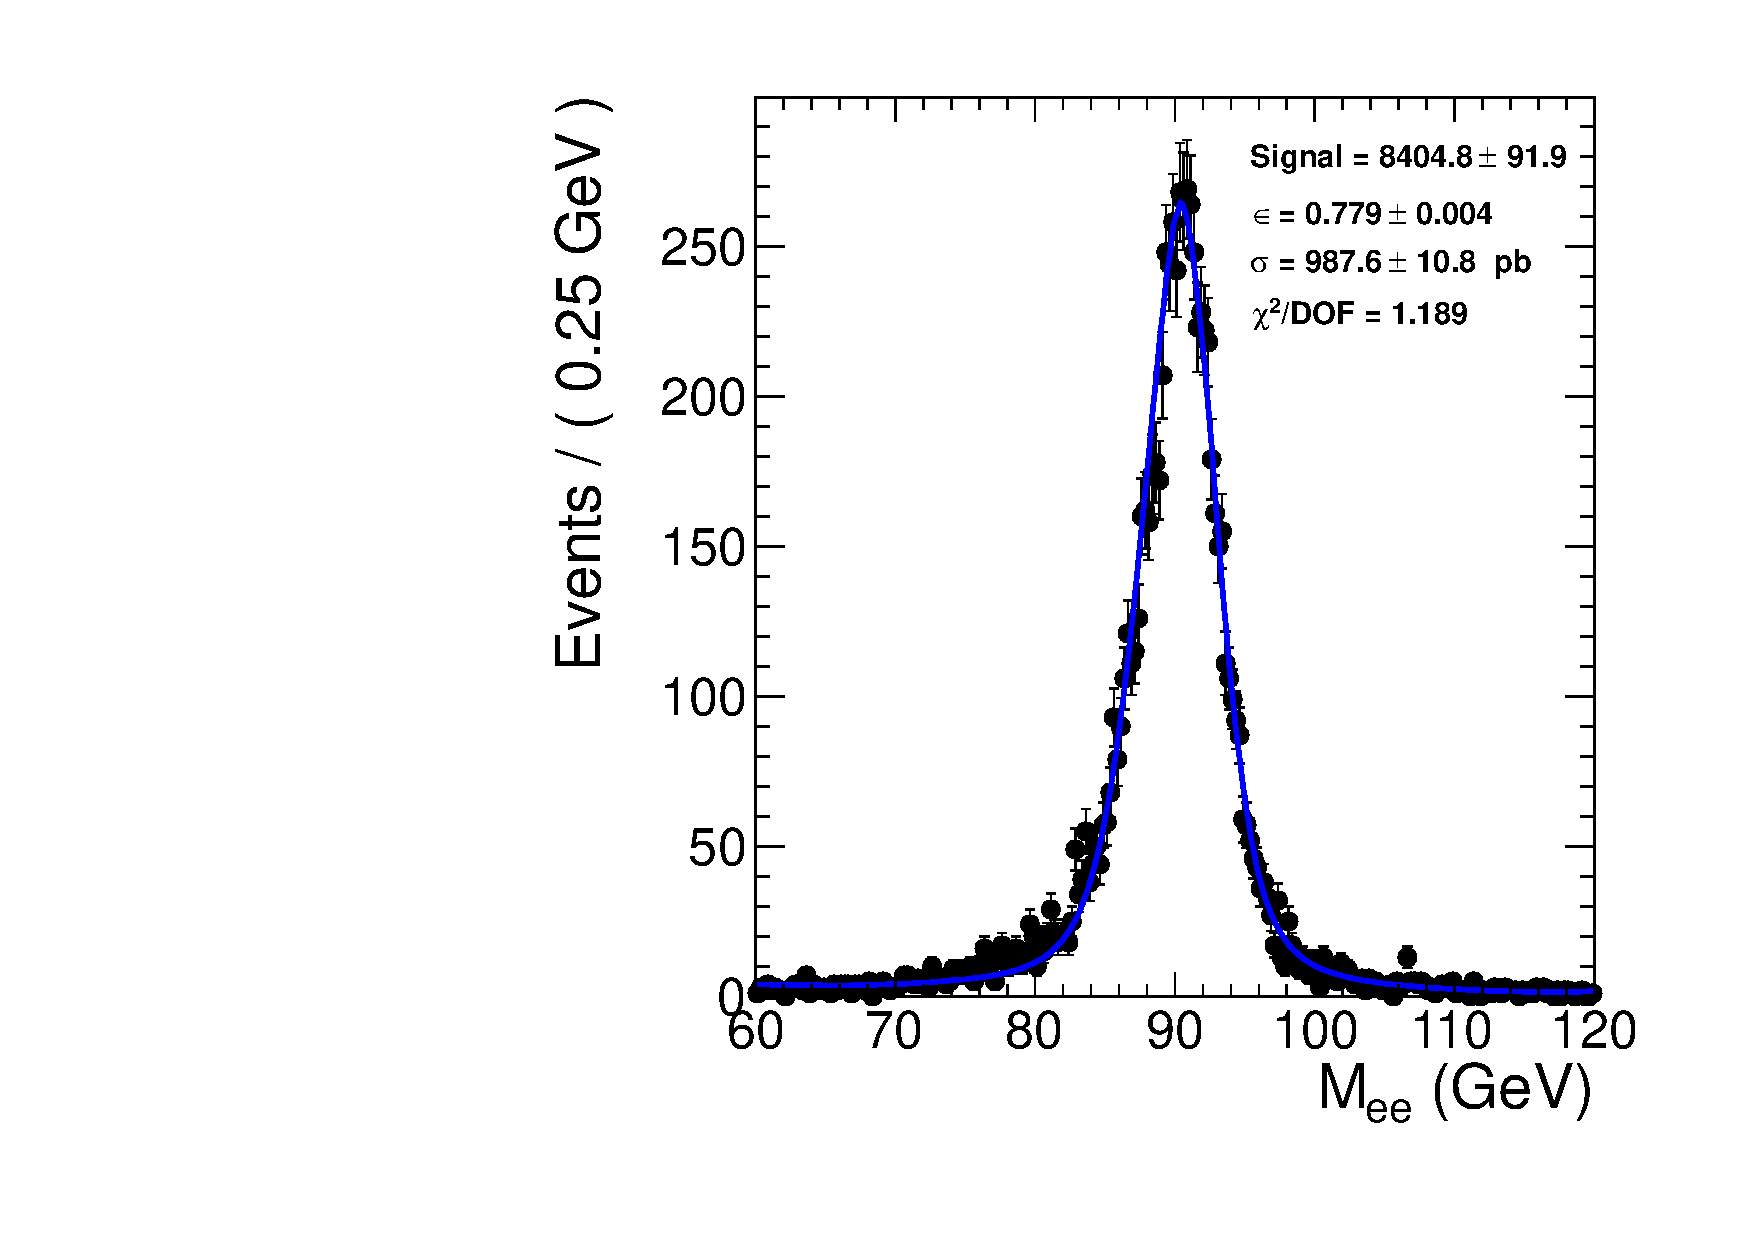
\includegraphics[width=0.48\textwidth]{figs/Zmass_TT_36143nb.pdf}
%   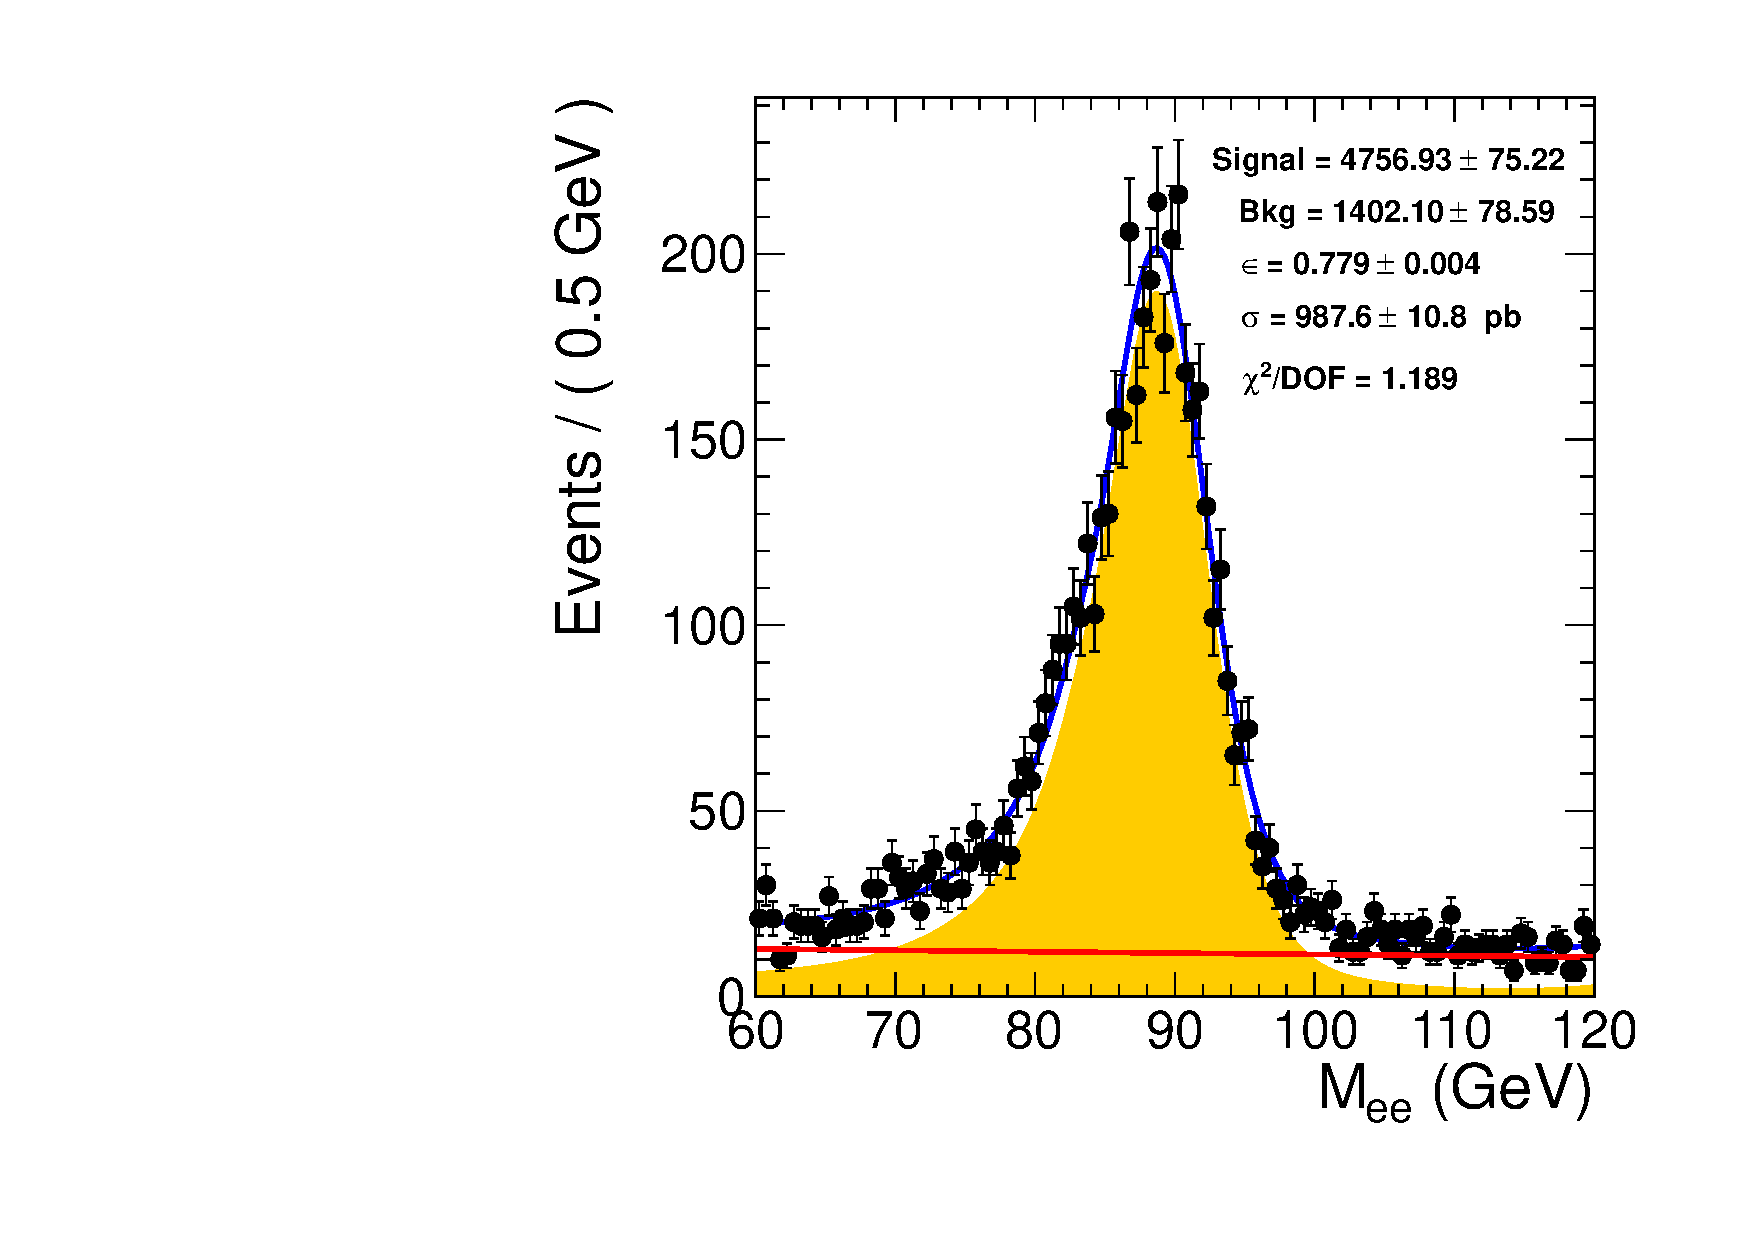
\includegraphics[width=0.48\textwidth]{figs/Zmass_TF_36143nb.pdf}
%   \caption{ \label{fig:Zmass_TT_TF}
%Fits to the Tag-Tag mass distributions (left plot) and Tag-Fail mass distributions (right plot)
%used in the simultaneous determination of the Zee yield and the electron efficiencies. }
%  \end{center}
%\end{figure}

%The electron $p_T$ distribution for $\Zee$ is shown in
%Fig.~\ref{fig:ZpT} in Appendix~\ref{sec:KinDist}.  Also,
%Fig.~\ref{fig:Zkin} shows the dielectron transverse
%momentum ($q_T$) and rapidity ($Y$) distributions.




\subsection{\texorpdfstring{The $\Zmm$ Signal Extraction}{The Z->mu mu Signal Extraction}}
\label{sec:Zmumu}

The yield of the $\Zmm$ events is determined from a fit simultaneously with the
average muon reconstruction efficiencies in the tracker and in
the muon detector, the muon trigger efficiency,
as well as the efficiency of the applied isolation requirement.
\Zmm candidates are obtained as pairs of muon candidates of different types
and organized into categories according to different requirements:
\begin{itemize}
\item $\Zmumu$: a pair of isolated global muons, further split into two samples:
\begin{itemize}
\item $\ZmumuTwoHlt$: each muons associated with an HLT trigger muon;
\item $\ZmumuOneHlt$: only one of the two muons associated with an HLT trigger muon;
\end{itemize}
\item $\Zmus$: one isolated global muon and one isolated
  stand-alone muon;
\item $\Zmut$: one isolated global muon and one isolated tracker track;
\item $\ZmumuNonIso$: a pair of global muons, of which one is isolated and the
other is nonisolated.
\end{itemize}

%The $\Zmumu$ category is also referred to as ``golden'' sample.
With the exception of the $\ZmumuOneHlt$ category, each global muon must correspond to an HLT trigger muon.
The five categories are explicitly forced to be mutually exclusive in the event
selection: if one event falls into the first category it is excluded from the second;
if it does not fall into the first category and falls into the second, it is excluded
from the third, and so on. In this way non-overlapping, hence statistically
independent, event samples are defined. The expected number of events in which more than
one dimuon combination is selected is almost negligible.
In those few cases all possible combinations are considered.

The five signal yields in each category can be written in terms of
the five unknowns, the Z signal yield $\NZtomumu$ and four efficiency terms, as follows:
\begin{eqnarray}
 \label{eqNmumuTwoHlt}
   \NmumuTwoHlt & = & \NZtomumu \effHlt^2 \effIso^2 \effTrk^2 \effSa^2,  \\
  \label{eqNmumuOneHlt}
   \NmumuOneHlt & = & 2 \NZtomumu \effHlt (1 - \effHlt) \effIso^2 \effTrk^2 \effSa^2,  \\
  \label{eqNmus}
   \Nmus & = & 2 \NZtomumu \effHlt \effIso^2 \effTrk (1 - \effTrk) \effSa^2,  \\
  \label{eqNmut}
   \Nmut & = & 2 \NZtomumu \effHlt \effIso^2 \effTrk^2 \effSa(1 -\effSa), \\
  \label{eqNmumuNonIso}
   \NmumuNonIso & = & 2 \NZtomumu \effHlt^2  \effIso (1 - \effIso)  \effTrk^2 \effSa^2.
\end{eqnarray}
The various efficiency terms in Eqs.~(\ref{eqNmumuTwoHlt}) to~(\ref{eqNmumuNonIso}),
the average efficiencies
of muon reconstruction in the tracker, $\effTrk$, in the muon detector as
a stand-alone muon, $\effSa$, the average efficiency of the isolation requirement,
$\effIso$, and the average trigger efficiency, $\effHlt$,
can be factorized because the muon selection
factorizes the requirements on the tracker and muon detector quantities separately.
Neither selection on $\chi^2$ per degree of freedom nor requirement of the muon reconstruction through the
tracker-muon algorithm is applied in order to
avoid efficiency terms that cannot be described as a product of contributions from the tracker and
the muon detector.
%We verified on Monte Carlo that the possible effects of any residual correlation
%can be either incorporated in the proper definition of the efficiencies or
%is negligible.
% Above, $\effTrk$ is
% the efficiency to reconstruct a track {\it and} to pass the track selection,
% and $\effSa$ is the efficiency to reconstruct a track in the muon detector {\it and} to pass the
% stand-alone muon selection, according to the selection described in Section~\ref{sec:muonid}.

The dimuon invariant mass spectra for the five categories are divided into
bins of different sizes, depending on the number of observed events.
The distributions of the dimuon invariant mass for the different categories can be written
as the sum of a signal peak plus a background component.


Figure~\ref{fig:zGolden36pb} shows the dimuon invariant mass spectrum for the $\Zmm$ golden events
on both a linear scale and a logarithmic scale, and Figs.~\ref{fig:zNoGold1}
and~\ref{fig:zNoGold2} show the
invariant mass distributions for the remaining categories.
The spectra are in agreement with the simulation.

\begin{figure}[hbtp]
    \begin{minipage}{73mm}
      \begin{center}
%        \resizebox{1.0\textwidth}{!}{{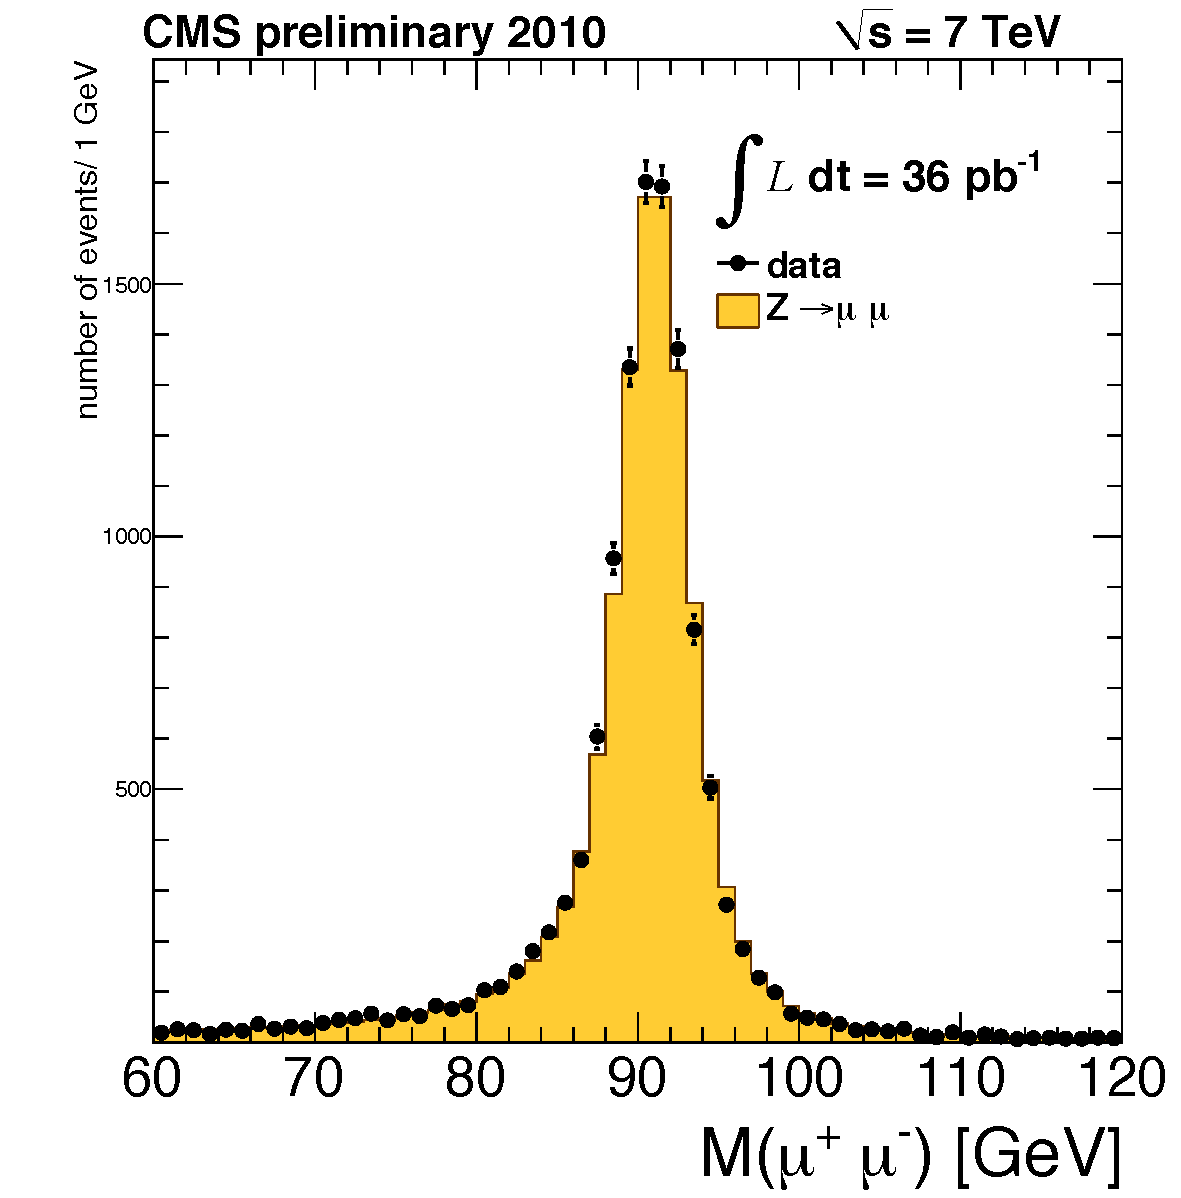
\includegraphics{figs/zGoldenLin_36pb.pdf}}}
        \resizebox{1.0\textwidth}{!}{{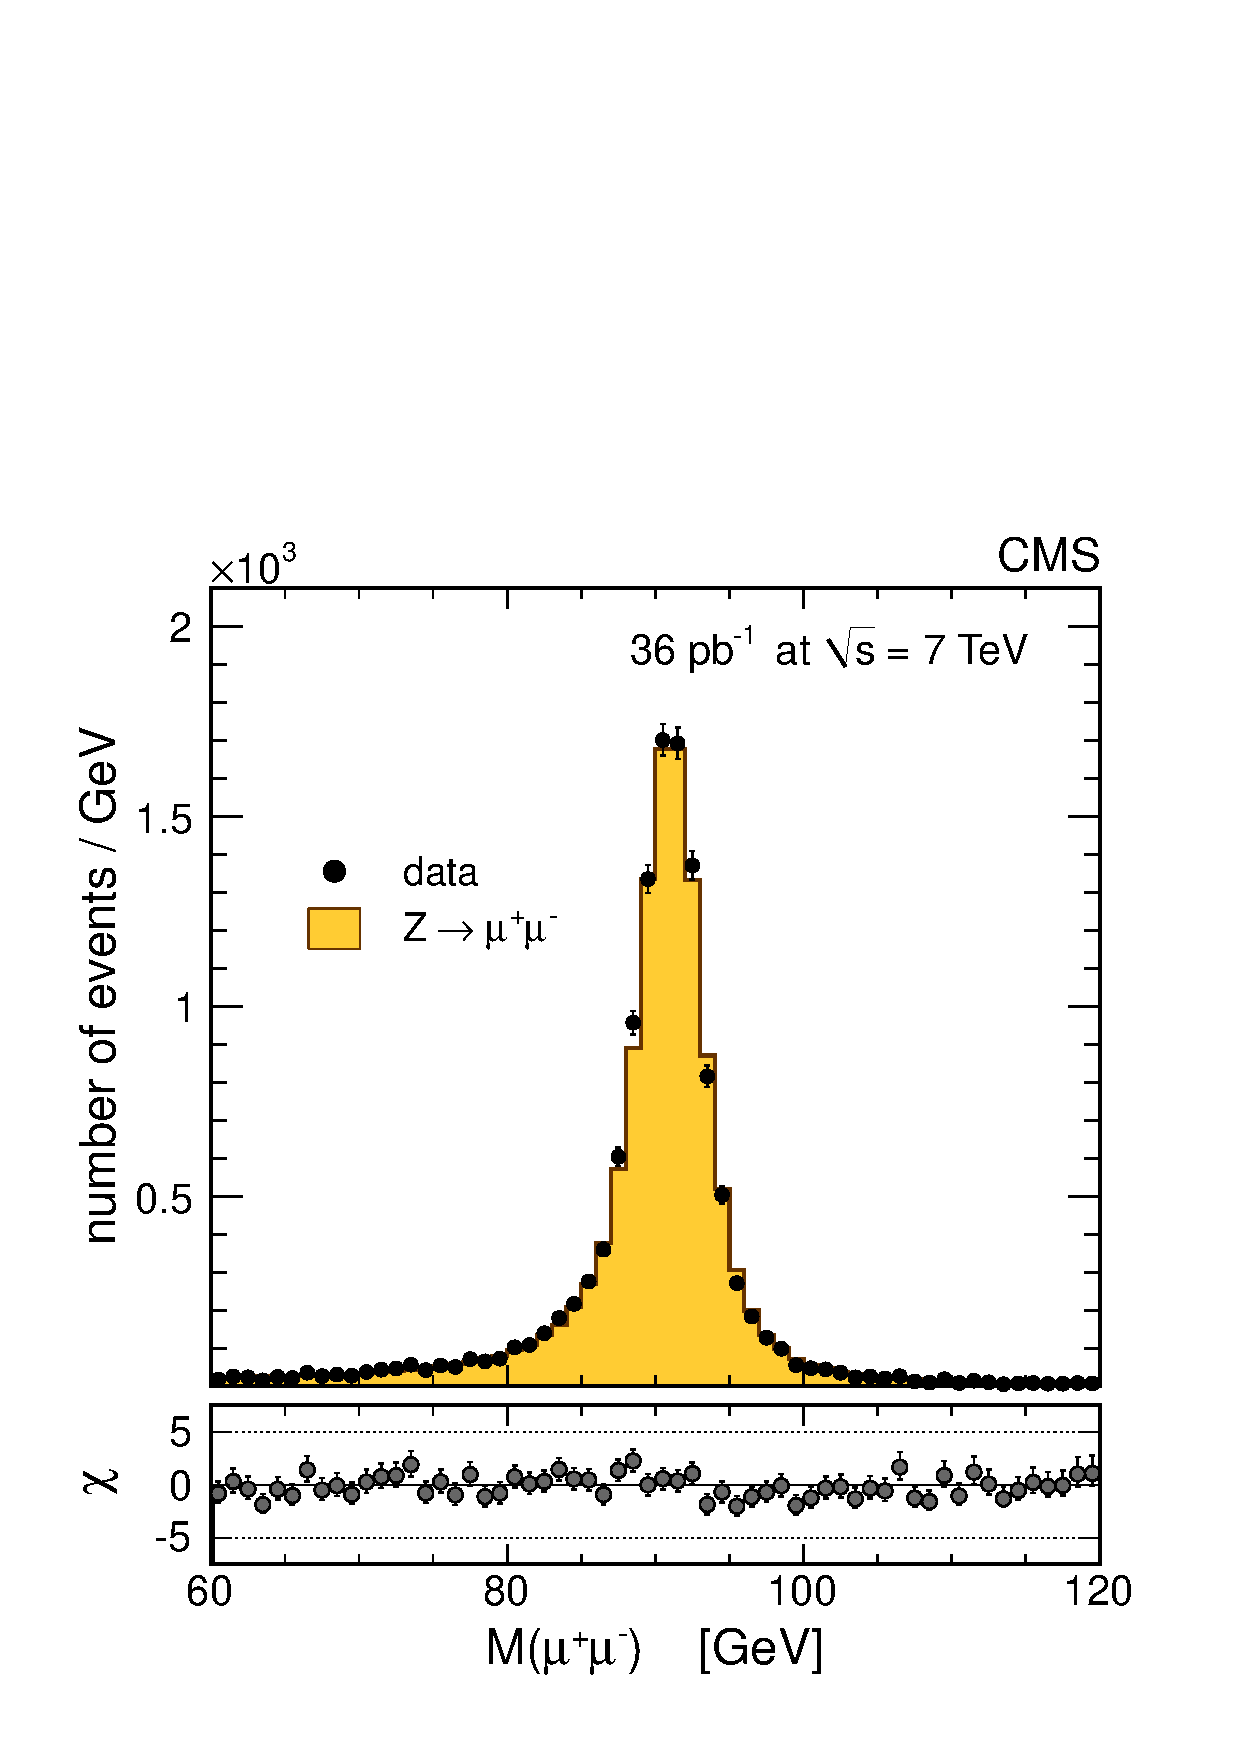
\includegraphics{figs/Zmumu_lin.pdf}}}
      \end{center}
    \end{minipage}
    \begin{minipage}{73mm}
       \begin{center}
%       \resizebox{!}{1.0\textwidth}{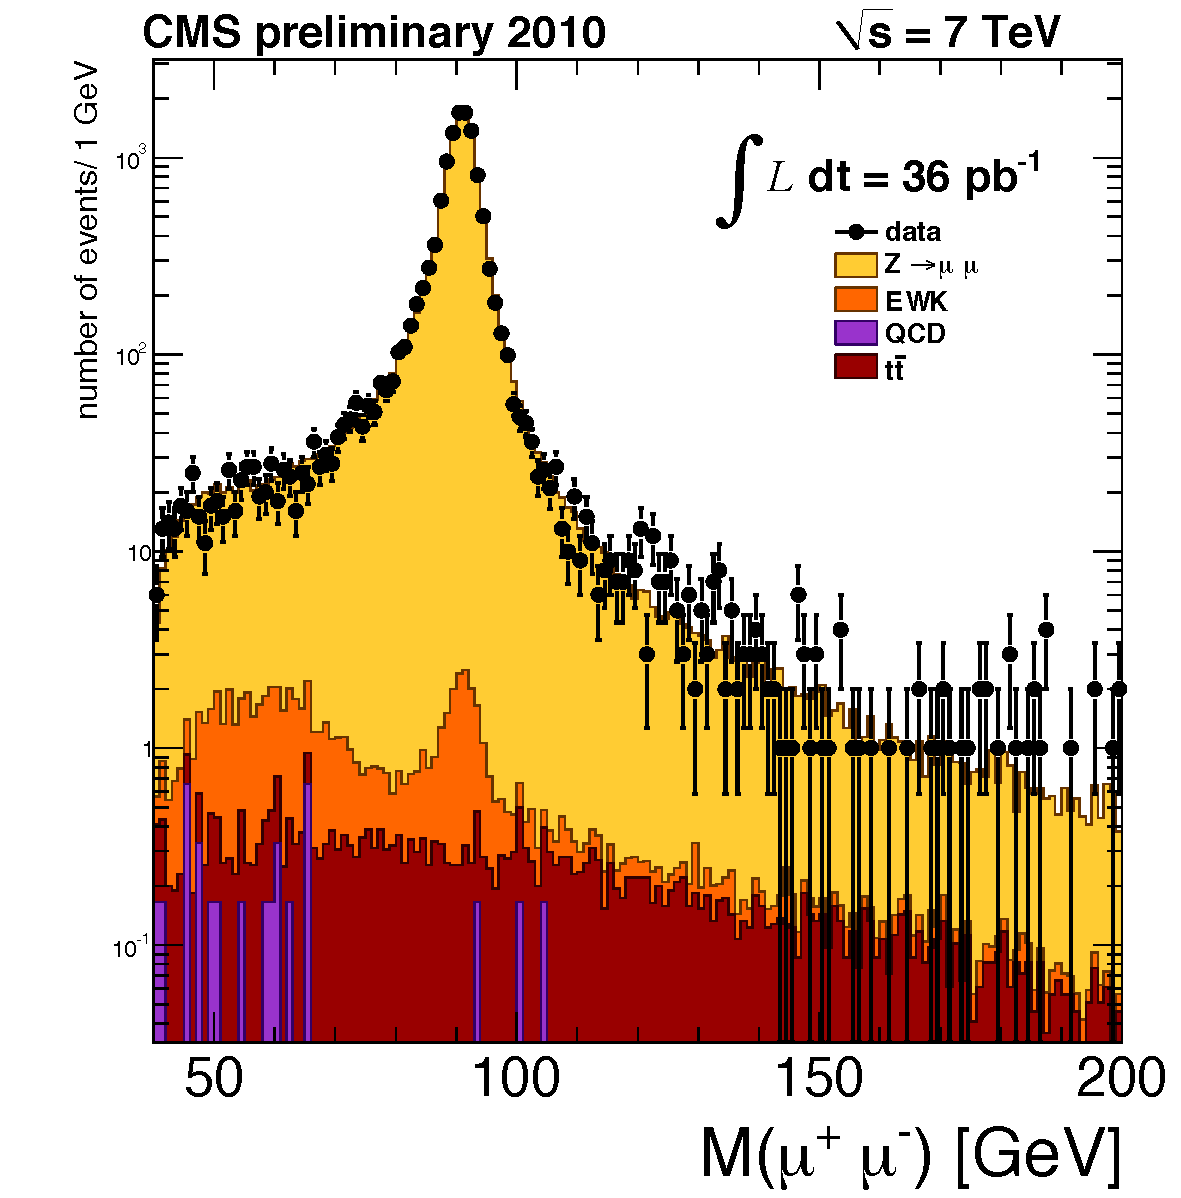
\includegraphics{figs/zGoldenLog_36pb.pdf}}
       \resizebox{!}{1.0\textwidth}{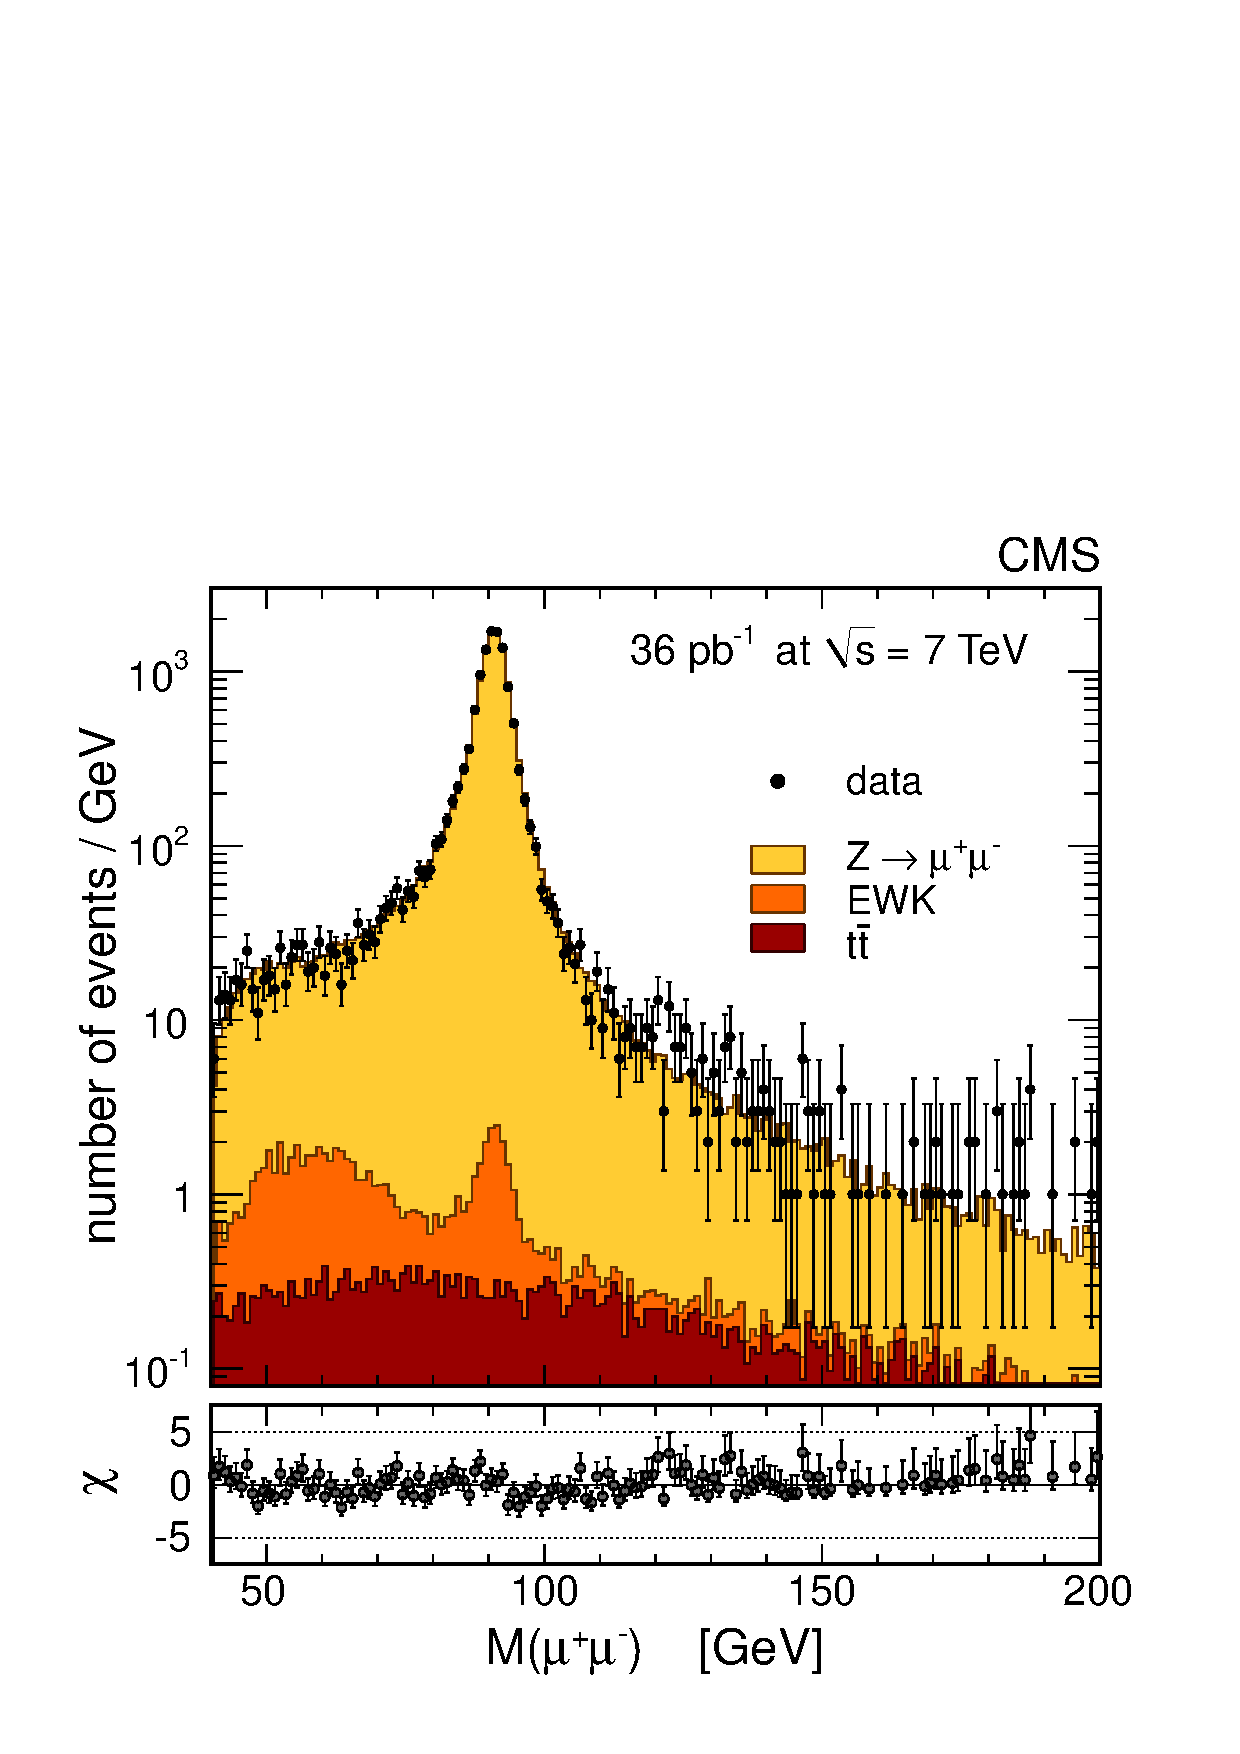
\includegraphics{figs/Zmumu_log.pdf}}
      \end{center}
    \end{minipage}
\caption{
Distributions of the dimuon invariant mass for the selected $\Zmm$ golden candidates on
a linear scale (left) and on a logarithmic scale (right).
The points with the error bars represent the data.
Superimposed are the expected distributions from simulations, normalized
to an integrated luminosity of $36$~pb$^{-1}$. The expected distributions are
the Z signal (yellow, light histogram), other EWK processes (orange, medium histogram),
and $\ttbar$ background (red, dark histogram).
Backgrounds are negligible and cannot be seen on the linear-scale plots.
}
\label{fig:zGolden36pb}
\end{figure}

\begin{figure}[hbtp]
    \begin{minipage}{73mm}
      \begin{center}
        \resizebox{1.0\textwidth}{!}{{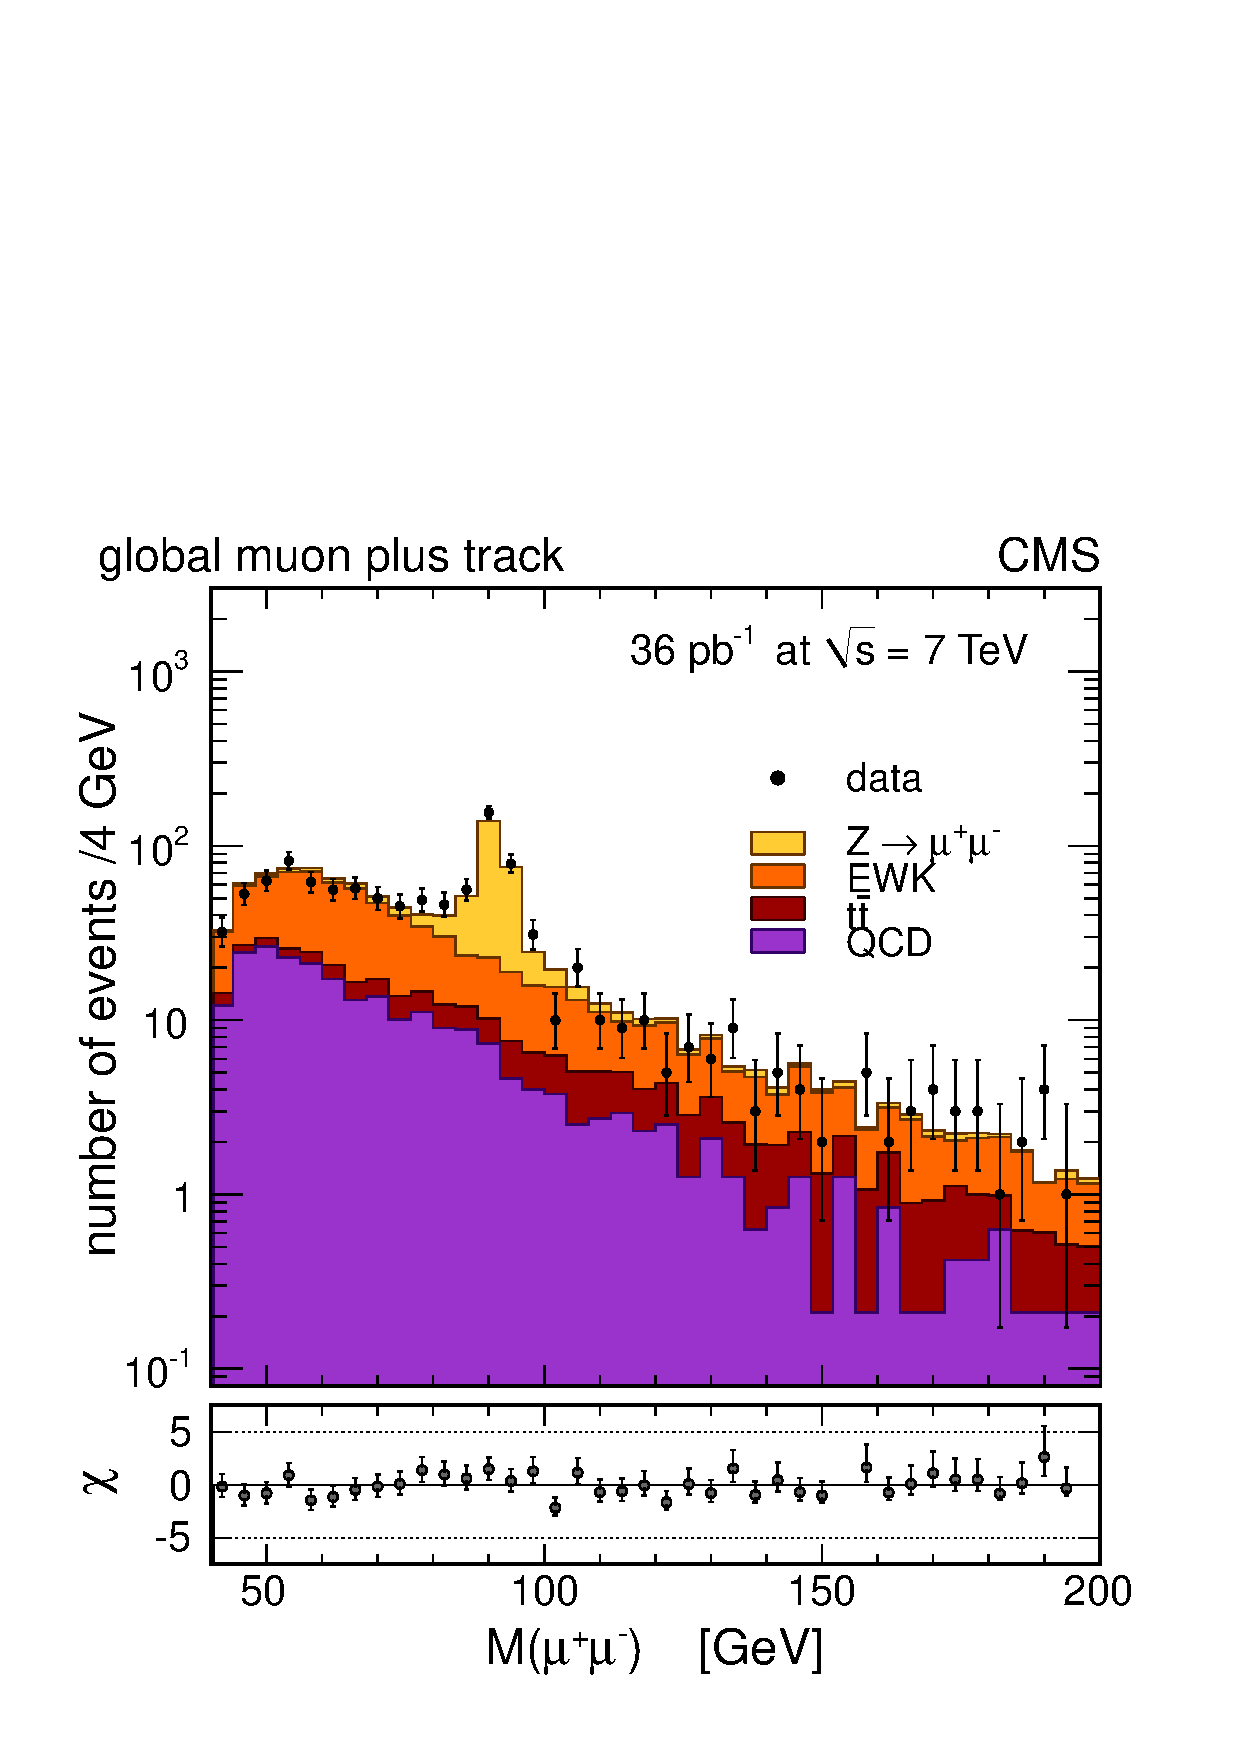
\includegraphics{figs/ZMuTrk_log.pdf}}}
      \end{center}
    \end{minipage}
    \begin{minipage}{73mm}
       \begin{center}
       \resizebox{!}{1.0\textwidth}{\includegraphics{figs/ZMuSta_log.pdf}}
      \end{center}
    \end{minipage}
\caption{Distributions of the dimuon invariant mass for the selected
$\Zmut$ (left) and $\Zmus$ (right) candidates.
The points with the error bars represent the data.
Superimposed are the expected distributions from simulations, normalized
to an integrated luminosity of $36$~pb$^{-1}$. The expected distributions are
the Z signal (yellow, light histogram), other EWK processes (orange, medium histogram),
$\ttbar$ background (red, dark histogram) and QCD background (violet, black histogram).
}
\label{fig:zNoGold1}
\end{figure}
\begin{figure}[hbtp]
    \begin{center}
     \begin{minipage}{73mm}
       \begin{center}
        \resizebox{!}{1.0\textwidth}{\includegraphics{figs/ZNotIso_log.pdf}}
       \end{center}
     \end{minipage}
   \end{center}
\caption{Distributions of the dimuon invariant mass for the selected
$\ZmumuNonIso$ candidates.
The points with the error bars represent the data.
Superimposed are the expected distributions from simulations, normalized
to an integrated luminosity of $36$~pb$^{-1}$. The expected distributions are
the Z signal (yellow, light histogram), other EWK processes (orange, medium histogram),
$\ttbar$ background (red, dark histogram), and QCD background (violet, black histogram).
}
\label{fig:zNoGold2}
\end{figure}

%, and the background can be considered
%negligible in the 'golden' categories (of the order of few per mille).
% \begin{eqnarray}
%    \NmumuTwoHlt (m) & = & \NmumuTwoHlt f_{peak}(m)\,, \\
%    \NmumuOneHlt (m) & = & \NmumuOneHlt f_{peak}(m)\,, \\
%    \Nmus (m) & = & \Nmus f^s_{peak}(m) + b_{\mu s}(m)\,, \\
%    \Nmut (m) & = & \Nmut f_{peak}(m) + b_{\mu t}(m)\,, \\
%    \NmumuNonIso (m) & = & \NmumuNonIso f_{peak}(m) + b_{\mu\mu}^{\mathrm{non\,iso}}(m)\,. \\
% \end{eqnarray}
The signal-peak distribution can be considered to be identical in the categories
$\Zmumu$ and $\Zmut$  because the momentum resolution in CMS is determined predominantly
by the tracker measurement for muons with $\Pt \leq 200$ GeV.
The binned spectrum of the dimuon invariant mass in the
$\Zmumu$ category, which has the most events of all categories,
is taken as shape model for all categories but $\Zmus$.
The large size of the golden sample ensures that the statistical
uncertainty of the invariant mass distribution has a negligible effect on the cross
section measurement.
The small presence of background is neglected in this distribution.
The uncertainty due to this approximation has been evaluated and
taken as the systematic uncertainty as described in Section~\ref{sec:muonSyst}.

Because only tracker isolation is used, the shape obtained from golden events
can also be used to model the $\ZmumuNonIso$ peak distribution.
A requirement on calorimetric isolation would have distorted the dimuon invariant mass
distribution of events with one nonisolated muon because of FSR,
as has been observed both in simulation and data.

The model of the invariant mass shape for the $\Zmus$ category is also derived from golden dimuon events.
The three-momentum for one of the two muons is taken from only the muon detector track fit,
in order to emulate a stand-alone muon.
To avoid using the same event twice in forming the $\Zmus$ shape model,
the higher-$\Pt$ (lower-$\Pt$) muon is chosen for even (odd) event numbers.

Background shapes are modeled as products of an exponential times a polynomial
whose degree depends on the category.
% :
% \begin{eqnarray}
%   b_{\mu t}(m) & = & N^b_{\mu t} (1 + a_1 m + a_2 m^2) e^{-\alpha m} \\
%   b_{\mu\mu}^{\mathrm{non\,iso}}(m) & = &
%   N_{\mu\mu}^{b\,\,{\mathrm{non\,iso}}} (1 + b_1 m + b_2 m^2) e^{-\beta m} \\
%   b_{\mu s}(m) & = & N^b_{\mu s} (1 + c_1 m + c_2 m^2) e^{-\gamma m}
% \end{eqnarray}
Different background models and different binning sizes are considered for the
categories other than $\Zmumu$ and a systematic uncertainty related to the fitting
procedure is determined accordingly.

%  f_{peak}^{s}(m) & = & \frac{1}{\sqrt{2\pi\sigma_s^2}} e^{-\frac{(m - M)^2}{2 \sigma_s^2} } \\
%The peak function for the $\Zmus$ category, $f_{peak}^{s}(m)$, is modeled as a
%Gaussian, due to the poor resolution, and the low statistics in that sample:

A simultaneous binned fit based on a Poissonian likelihood~\cite{PoisLR} is performed
for the different categories.
%We define, for each category, minus two times the negative logarithmic
%of the following Poissonian likelihood ratio~\cite{PoisLR}:
% \begin{equation}
% \chi^2_{\lambda} = -2 \ln{\lambda(m)} =  -2 \ln{\frac{\mathrm{Poiss}(n_i,
%     \nu_i)}{\mathrm{Poiss}(n_i, n_i)}} = \sum_{i=1}^{n_{\mathrm{bins}}} \nu_i - n_{i} + n_i \log{\frac{n_i}{\nu_i}}\,,
% \end{equation}
% where $\nu_i$ is the expected number of events in the $i^{\mathrm{th}}$-bin in $m$,
% $n_i$ is the measured number of events in that
% bin, and $\mathrm{Poiss}(n,\nu)$ is a Poissonian distribution.
% The simultaneous fit is performed minimizing the sum $R$ of the five $\chi^2_\lambda,j$ from
% the different categories $j=1,\cdots, 5$, i.e.:
% \begin{equation}
% R =  \sum_{j=1}^{5} \chi^2_{\lambda,j}   = 2  \sum_{j=1}^{5} \sum_{i=1}^{n_{\mathrm{bins}}^{(j)}} \nu^{(j)}_i - n^{(j)}_{i} + n^{(j)}_i \log{\frac{n^{(j)}_i}{\nu^{(j)}_i}}\,.
% \label{eq:PoisLR}
% \end{equation}
% For sufficiently large $\nu_i$, as in our case, the minimum of $R$ follows with good approximation a $\chi^2$ distribution,
% allowing a goodness-of-fit test.
% Using only the number of events for the two categories with the largest statistics,
% $\ZmumuTwoHlt$ and $\ZmumuOneHlt$, the Z yield and the four efficiencies can be obtained minimizing the
% following expression, which can be obtained from Eq.~\ref{eq:PoisLR} using a single bin in the Gaussian approximation for $\ZmumuTwoHlt$
% and $\ZmumuOneHlt$:
% \begin{eqnarray*} \label{chi2}
% R & = &
% \frac{(\NmumuTwoHlt - \NZtomumu\effHlt^2\effIso^2\effTrk^2\effSa^2)^2}{\NmumuTwoHlt} +  \\
% & & \frac{(\NmumuOneHlt - 2\NZtomumu\effHlt(1-\effHlt)\effIso^2\effTrk^2\effSa^2)^2}{\NmumuOneHlt} +  \\
% & & \chi^2_{\lambda, \mu s} +
% \chi^2_{\lambda, \mu t} +
% \chi^{\nonIso\,\, 2}_{\lambda, \mumu}\, ,
% \end{eqnarray*}
% where we use the event counts only in the  $\ZmumuOneHlt$ and $\ZmumuTwoHlt$ 'golden'
% categories and the Poissonial terms $\chi^2_{\lambda, \mu s}$, $\chi^2_{\lambda, \mu t}$ and
% $\chi^{\nonIso\,\, 2}_{\lambda, , \mumu}$ for the remaining categories.
% The likelihood ratio fit is equivalent to an ordinary $\chi^2$
% for sufficiently large statistics and we verified that, with the current data sample,
% it gives the same central value and statistical uncertainty.
%We perform the fit in the range $60 < m < 120~\mathrm{GeV}/c^2$.
%Full details on the signal and background modeling assumptions and
%correlation studies are present in~\cite{CMS_AN_2010-345}.
Table~\ref{fig:fitRes_36pb} reports the signal yield and single-muon efficiencies determined from
the simultaneous fit and the ratios of the fitted to simulation efficiencies.
A goodness-of-fit test gives a probability ($p$-value) of 0.36 for this fit.

%The resulting fit $p$-value shows the good quality of the fit.
%With the analyzed statistics, a second degree polynomial function is
%taken for modeling  the background shape.

\begin{table}[htbp] %L.L.
\begin{center}
\caption{Signal yield and efficiencies determined from data with the simultaneous fit, and
  ratios of efficiencies determined from the fit and the simulation.}
\label{fig:fitRes_36pb}
\begin{tabular}{|c|c|c|}
\hline
Quantity & Fit results from data & Data/simulation\\
\hline\hline
$\NZtomumu$ &13\,728 $\pm$ 121   & \\
\hline
$\effHlt$ & 0.9203 $\pm$ 0.0019  &0.9672 $\pm$ 0.0020   \\
$\effIso$ & 0.9813 $\pm$ 0.0010& 0.9962 $\pm$  0.0011 \\
$\effSa$ & 0.9762  $\pm$ 0.0012 & 0.9964 $\pm$ 0.0013 \\
$\effTrk$ & 0.9890 $\pm$ 0.0006  & 0.9949 $\pm$ 0.0007  \\
\hline
\end{tabular}
\end{center}
\end{table}

%In order to correct the fitted yield $\NZtomumu$ for the presence of background,
%the estimated irreducible background fraction is subtracted.
%$f_{bkg}=0.44 \pm 0.02\%$.

The background in the $\Zmumu$ golden category (of the order of few per mille)
was neglected in the fit. In order to correct the fitted yield $\NZtomumu$ for
the presence of this background, we subtract the small estimated irreducible
background fraction.

A $(1.0\pm 0.5)\%$ overall efficiency correction due to the loss of muon events because of trigger
prefiring is also applied (Section~\ref{sec:muonEff}).

The estimated cross section is $968\pm 8 \mathrm{(stat.)}$~pb.

As cross-check, a simpler analysis based on event counting was also performed.
The same selection was applied, and the number of events with two global muon, reported
in Sec~\ref{sec:muonid}, was used as signal yield. 
The signal yield was then corrected for the relevant efficiencies that have 
been evaluated with a \TNP method in a single $\Pt$ and $\eta$ bin, resulting in a
cross section estimate of $969\pm 8 \mathrm{(stat.)}$~pb, in good agreement
with the simultaneous fit method.


\section{Systematic Uncertainties}
\label{sec:systematics}

The largest uncertainty contribution on the measured cross sections is related to the
integrated luminosity~\cite{lumiPAS}, and amounts to $\LUMISYST\%$.
\par
The next most important source of systematic uncertainty is due to the
lepton efficiency correction factors obtained
from the \TNP method.
In the $\Zmm$ analysis, the efficiency uncertainties are 
absorbed in the statistical uncertainty of the measurement, via the simultaneous 
fit to the yield and efficiencies.

%The $\MET$ energy scale is affected by our limited knowledge of the intrinsic hadronic recoil response. 
%We observe minor discrepancies when comparing hadronic recoil distributions in data and simulation, 
%and assign uncertainties of $\WEIMETSYST\%$ and $\WMIMETSYST\%$ to $\Wen$ and $\Wmn$ cross sections
%respectively.

Table~\ref{tab:syst} shows a summary of systematic uncertainties
for the $\Wo$ and $\Zo$ cross section measurements.
Tables~\ref{tab:systEL} and~\ref{tab:systMU}
show a summary of systematic uncertainties
for the individual cross sections ($\Wp, \Wm$) and the ratios ($\Wp/\Wm$, $\Wo/\Zo$).
Details of systematic uncertainties for the muon and electron channels are described in the
following subsections.

\begin{table}[htbp] %
\begin{center}
   \caption[.]{ \label{tab:syst}
Systematic uncertainties in percent for inclusive W and Z cross sections.
The ``n/a'' entry means that the source does not apply.
A common luminosity uncertainty of 4\% applies to all channels.}
\begin {tabular} {|l|c|c|c|c|}
\hline
Source                                   & $\Wen$         & $\Wmn$           & $\Zee$         & $\Zmm$ \\
\hline\hline
Lepton reconstruction \& identification  & \WEITNPSYST    & \WMIEFFSYST      & \ZEETNPSYST    &  n/a \\
Trigger prefiring                      & n/a            & \WMIEFFPRET      & n/a            & \ZMMEFFPRET \\
Energy/momentum scale \& resolution             & \WEIESCALESYST & \WMISCALESYST    & \ZEEESCALESYST & \ZMMSCALESYST \\
$\MET$ scale \& resolution               & \WEIMETSYST    & \WMIMETSYST      &  n/a           &  n/a   \\
Background subtraction / modeling        & \WEIBKGSYST    & \WMIQCDSHAPESYST & \ZEEBKGSYST    & \ZMMBKGTOTSYST  \\
Trigger changes throughout 2010          & n/a            & n/a              & n/a            & \ZMMTRIGABSYST \\
\hline
Total experimental                       & \WEEXPSYST    & \WMEXPSYST       & \ZEEEXPSYST    & \ZMMEXPSYST \\
\hline
PDF uncertainty for acceptance           & \WEIPDFACCSYST & \WMIPDFACCSYST   & \ZEEPDFACCSYST & \ZMMPDFACCSYST \\
Other theoretical uncertainties          & \WEITHSYST     & \WMITHSYST       & \ZEETHSYST     & \ZMMTHSYST  \\
\hline
Total theoretical                        & \WEITOTTHSYST & \WMITOTTHSYST & \ZEETOTTHSYST & \ZMMTOTTHSYST \\
\hline
Total (excluding luminosity)                      & \WEITOTSYST    & \WMITOTSYST      & \ZEETOTSYST    & \ZMMTOTSYST \\
\hline
\end {tabular}
\end{center}
\end{table}


\begin{table}[htbp] %
\begin{center}
   \caption[.]{ \label{tab:systEL}
Systematic uncertainties in percent for individual W cross sections and the ratios in the
electron channel.
A common luminosity uncertainty of 4\% applies to all cross sections. }
\begin {tabular} {|l|c|c|c|c|}
\hline
Source       & $\Wp$ (e) & $\Wm$ (e) & $\Wp/\Wm$ (e) & $W/Z$ (e) \\
         \hline\hline
Lepton reconstruction \& identification  & 1.4 & 1.4 & 1.5 & 1.1 \\
Energy scale \& resolution               & 0.5 & 0.6 & 0.1 & 0.2 \\
$\MET$ scale \& resolution               & 0.3 & 0.3 & 0.1 & 0.3 \\
Background subtraction / modeling        & 0.3 & 0.5 & 0.4 & 0.3 \\
\hline
Total experimental                       & 1.5 & 1.6 & 1.6 & 1.2 \\
\hline
PDF uncertainty for acceptance           & 0.7 & 1.2 & 1.6 & 0.6 \\
Other theoretical uncertainties          & 1.0 & 0.7 & 1.2 & 1.2 \\
\hline
Total theoretical                        & 1.2 & 1.4 & 2.0 & 1.4 \\
\hline
Total (excluding luminosity)             & 2.0 & 2.1 & 2.6 & 1.8 \\
\hline
\end {tabular}
\end{center}
\end{table}

\begin{table}[htbp] %
\begin{center}
   \caption[.]{ \label{tab:systMU}
Systematic uncertainties in percent for individual W cross sections and ratios in the
muon channel.
A common luminosity uncertainty of 4\% applies to all cross sections. }
\begin {tabular} {|l|c|c|c|c|}
\hline
Source       & $\Wp$ ($\mu$) & $\Wm$ ($\mu$) & $\Wp/\Wm$ ($\mu$) & $W/Z$ ($\mu$) \\
         \hline\hline
Lepton reconstruction \& identification  & 0.9 & 0.9 & 1.3 & 0.9 \\
Trigger prefiring                       & 0.5 & 0.5 & 0   & 0   \\
Momentum scale \& resolution             & 0.19 & 0.25 & 0.06 & 0.35 \\
$\MET$ scale \& resolution               & 0.2 & 0.2 & 0.0   & 0.2 \\
Background subtraction / modeling        & 0.4 & 0.5 & 0.2 & 0.4 \\
\hline
Total experimental                       & 1.1 & 1.2 & 1.3 & 1.1 \\
\hline
PDF uncertainty for acceptance           & 0.9 & 1.5 & 1.9 & 0.9 \\
Other theoretical uncertainties          & 0.9 & 0.8 & 0.8 & 1.4 \\
\hline
Total theoretical                        & 1.3 & 1.7 & 2.1 & 1.6 \\
\hline
Total (excluding luminosity)                             & 1.7 & 2.1 & 2.5 & 2.0 \\
\hline
\end {tabular}
\end{center}
\end{table}
%------------------------------------------------------------




\subsection{Electron Channels}
\label{subsec:ELEsystematics}

\par
The propagation of statistical and systematic uncertainties on the data/simulation
efficiency correction factors ($\rhoeff$)
from the \TNP method (reconstruction, identification, and trigger)
results in uncertainties of $\WEITNPSYST\%$ and $\ZEETNPSYST\%$ for the $\Wen$ and $\Zee$ analyses,
respectively. The uncertainties on the $\Wp$ and $\Wm$ cross sections are larger than that for
the inclusive $\Wo$ because of the larger statistical uncertainty when efficiencies are estimated
per charge. The systematic uncertainty, which depends on the efficiency
under study, is determined by considering alternative signal and background models. 
The size of the systematic uncertainty is 0.3$\%$ for the electron selection efficiencies 
and 1.0$\%$ for the electron reconstruction efficiency. The estimation of the 
trigger efficiency is considered to be background-free so there is no need to 
perform a fit for the signal estimation. Theoretical uncertainties on the 
corrected efficiencies related to the PDF uncertainties and the PDF choice were 
found to be negligible.

\par
The electron energy scale has an impact on the \ET distribution
for the signal. To study this effect, the
energy-scale corrections obtained
from the shift of the $\Zo$ mass peak
(Section~\ref{sec:e-escale}) are applied to electrons in the EB and EE
in simulation (before the $\Et$ requirement)
and  the missing $\Et$ is recomputed.
The obtained variations on the signal yield from the UML fit
are $\WEIESCALESYST\%$ for the inclusive $\Wo$, $\WEPESCALESYST\%$ for the $\Wp$, and
$\WEMESCALESYST\%$ for the $\Wm$ samples and $\WERESCALESYST\%$ on the
$\Wp/\Wm$ ratio.  All the charge-related studies (determination of individual $\Wp$ and $\Wm$
yields and $\Wp/\Wm$ ratio and associated systematic uncertainties)
include data/simulation
%charge misidentification scale factor of $\WPWMISID$, estimated from
charge misidentification scale factors, estimated from
the fraction of same-sign events in the $\Zee$ data and simulated samples.
\par
The energy scale of electrons has an impact on the $\Zo$ yield because of 
the $\Et>25~\GeV$ requirement on the two electrons and the mass window requirement.
Applying the energy-scale corrections
mentioned above to the EB and EE electrons and reprocessing the data, 
the $\Zo$~yield is decreased by 10~events ($\ZEESAMPLE \to \ZEESAMPLEN$).
A systematic uncertainty equal to this decrease of $\ZEEESCALESYST\%$
is assigned to the $\Zo$ signal yield.
%High statistics MC study shows that the effect
%of the energy scale on the $Z$ yield is $0.6\%$.
%This number is consistent with the increase of yields that
%we observe when applying energy scale corrections to electrons in the data,
%both for WP80 and WP95.
The energy-scale uncertainty for the $\Wo$ selection is included in the systematic uncertainty 
described in the previous paragraph. There, the systematic uncertainty 
is larger than that for the $\Zo$ selection because the energy scale also affects the 
$\MET$ shape used for the signal extraction.
The $\Wo$ selection itself is affected by the energy scale at the level of $0.12\%$.
\par
%By applying the additional smearing of the electron energy obtained
%for the same fit to the $\Zee$ data,
%the $\Wo$ yield  is changed by 0.02\% and the $\Zo$ yield, by 0.XX\%.
The \MET shape used in the $\Wo$ fits is also distorted
by energy resolution uncertainties; this induces a change in the $\Wo$ signal yield
by 0.02\%.

\par
%The \MET energy scale is affected by our limited knowledge
%of the intrinsic hadronic recoil response.  However impressive
%progress on this issue has been accomplished by \MET experts
%from studies
%of the hadronic recoil distributions against photons in $\gamma$-jet,
%leptons in $W$ and dileptons in $Z$ events~\cite{metPAS}.
%From the discrepancies found in these data/simulation comparisons,
%we estimate uncertainties due to the \MET energy scale of
%$\WEIMETSYST\%$ for inclusive $W$, $\WEPMETSYST\%$ for $W^+$, $\WEMMETSYST\%$ for
%$W^-$ yields, and of $\WERMETSYST\%$ for the $W^+/W^-$ ratio.



The \MET energy scale is affected by our limited knowledge of the intrinsic hadronic
recoil response. From the discrepancies found in the data/simulation
comparisons (Section~\ref{sec:WsignalMETtemplate}), uncertainties due to
the \MET energy scale are estimated to be 0.3\% for inclusive $\Wo$,
$\Wp$, and $\Wm$ yields, and 0.1\% for the $\Wp/\Wm$ ratio.

\par
The systematic uncertainties on the background subtraction
address the possible difference between the true background distribution
and the modified Rayleigh function that is used in the UML fit.
We make the assumption that any such difference can be accounted
for by an additional $\sigma_2$ parameter (defined in Section~\ref{sec:WQCDbkg}),
which affects the resolution at large values of \MET (below the signal).
The value of $\sigma_2$ is first determined for three samples: the control sample
in the data, the control sample in the QCD simulation, and the
selected sample in the QCD simulation. The values obtained are $\sigma_2=0.0009~\GeV^{-1}$,
$0.0010~\GeV^{-1}$, and $0.0007~\GeV^{-1}$, respectively for $\Wp$ and
$\sigma_2=0.0007~\GeV^{-1}$,
$0.0009~\GeV^{-1}$, and $0.0008~\GeV^{-1}$ for $\Wm$.
The three values of $\sigma_2$ are then fixed in turn, and $\sigma_0$ and $\sigma_1$
are set to their values from data to generate distributions (of the size
of our sample) with
the three-parameter function, which  we then fit with our nominal two-parameter
function. The maximal relative difference in the yields
is quoted as the systematic uncertainty on background subtraction: $\WEIBKGSYST\%$ for inclusive $\Wo$,
$\WEPBKGSYST\%$ for $\Wp$, $\WEMBKGSYST\%$ for $\Wm$, and $\WERBKGSYST\%$ for the ratio.

\par
In the following paragraphs we discuss the systematic uncertainties of 
the fixed shape and the ABCD methods which were also explored in order 
to cross check the extraction of the $\Wen$ signal. 
These uncertainties correspond to the specific methods and are not propagated
to the final cross section measurement reported in this paper. 

The systematic uncertainties on the background subtraction using fixed-shape 
distributions are summarized in Table~\ref{tab:FixedTempSyst}.  
The total uncertainty is taken as the sum in quadrature of 
the values in the table, giving 0.40\%.  
The total uncertainty is dominated by the uncertainty of the correction of the 
signal contamination in the control sample. This uncertainty is evaluated by 
propagating the uncertainty on the measured contamination using the \TNP technique. 
The statistical uncertainty of this evaluation is calculated using 
a large number of shapes in which the number of events is generated 
from a Poisson distribution with the mean equal to the number of events in the nominal shape. 
The signal yield under variation of the requirements used to define the control 
sample was also studied and found to be very stable with an RMS spread  
of 0.12\% for the range of selections considered. In order to take into 
account the observation of small residual correlations that are not corrected for,
an additional systematic uncertainty of 0.35$\%$ is assigned as a conservative estimate of their size.

\begin{table}[htbp] %
  \begin{center}
    \caption{Summary of systematic uncertainties for background modeling using 
fixed-shape distributions.}
    \label{tab:FixedTempSyst}
    \begin{tabular}{|l|c|}
      \hline
      Source of systematic uncertainty & Value \\
      \hline\hline
      MVA Correction & 0.05\% \\
      Signal contamination & 0.15\% \\
      Statistical fluctuations & 0.12\% \\
      Residual correlations & 0.34\% \\
      \hline
      Total & 0.40\% \\
      \hline
    \end{tabular}
  \end{center}
\end{table} 


\par
The systematic uncertainties on the signal extraction using the ABCD method
are summarized in Table~\ref{tab:ABCDEsyst}. The total uncertainty is
taken as the sum in quadrature of the individual components listed in the table,
and corresponds to 0.7$\%$.
The two most important sources of systematic uncertainty arise from the 
modeling of the signal shape. The largest of these (0.53$\%$) comes from 
the uncertainty on $\varepsilon_\mathrm{P}$, dominated by the statistical uncertainties 
in the \TNP method. Uncertainties on the electron energy scale, and hadronic 
recoil response and resolution affect the modeling of the $\MET$ distribution 
for the signal and together give rise to the second largest uncertainty (0.4$\%$).
The uncertainty coming from the modeling of electroweak backgrounds is 
estimated to be 0.2$\%$. The assumption that the fake electron efficiency to 
pass the $\MET$ boundary is independent of the relative track isolation leads 
to a small bias for which a correction is applied. The uncertainty on this 
correction gives rise to a very small error on the yield of 0.07$\%$. This is dominated 
by the uncertainty on the signal contamination of the anti-selected sample used 
to estimate the correction.

\begin{table}[hbtp] %
  \begin{center}
    \caption{Summary of systematic uncertainties for the ABCD method.}
    \label{tab:ABCDEsyst}
    \begin{tabular}{|l|c|}
      \hline
      Source of systematic uncertainty & Value \\
      \hline\hline
      Signal contamination in bias correction & 0.07\% \\
      EWK backgrounds & 0.20\% \\
      Tag-and-probe  & 0.53\% \\
      $\MET$ modeling  & 0.40\% \\
      \hline
      Total & 0.70\% \\
      \hline
    \end{tabular}
  \end{center}
\end{table}




The QCD background in the $\Zee$ channel is estimated, as discussed earlier, 
using the shape information of the relative track isolation distribution. 
The relative uncertainty (approximately 0.14$\%$) of the 
total Z yield is used as the systematic uncertainty. 



\subsection{Muon Channels}
\label{sec:muonSyst}

% Dedicated studies indicate a muon momentum scale effect of $(-0.09\pm 0.03)\%$ for 40 GeV muons.
% An upper limit on potential resolution effects of 0.12\% is also obtained.
% The effect of momentum scale uncertainty has been estimated to be $\WMISCALESYST\%$ for $\Wmn$ and
%  $\ZMMSCALESYST\%$ for $\Zmm$ respectively.

The total uncertainty of 0.9\%  (statistical plus systematic) on the 
correction factors $\rhoeff$ is used as the systematic uncertainty due to muon efficiency 
(reconstruction, identification, selection, isolation,
and trigger) for the $\Wmn$ yield. 
%
% Removed from comments by Isabel (L.L.)
%
%Additionally, the variation of the correction factors with different PDF
%assumptions for the simulated Z samples, used to evaluate the 
%\TNP efficiencies in simulations, has been evaluated
%as $0.01\%$ and therfore has been neglected.
The systematic uncertainty assigned to the efficiencies is evaluated using
a large simulated sample including the Z signal and all potential backgrounds. 
Additional uncertainties are evaluated by varying the initial Z preselection criteria and
the mass window to perform the background subtraction fit, and by using alternative parameterizations to model the 
background. The statistical uncertainties on the fit parameters describing the background correction 
are also included. The effect of the uncertainties due to the choice of PDFs used in the Z simulation is also studied and found to 
be negligible.

%The full difference in correction factors for the positively and negatively charged muons, 1.3\%, 
%is propagated as a systematic uncertainty in the measurement of the $\Wp/\Wm$ cross-section ratio.

A conservative systematic uncertainty of 0.5\%, due to the correction for the trigger prefiring inefficiency 
(Section~\ref{sec:muonEff}), is assigned to both the $\Zmm$ and $\Wmn$ cross-section estimates.

Dedicated studies comparing the peak position and width of the observed Z distribution
with the expected one indicate a muon momentum scale effect of ${\sim} 0.25\%$ for 40 GeV muons.
In order to evaluate the impact on the W cross-section measurement,
the fitting procedure with a new signal distribution where the muon $\Pt$ in the simulations
is modified according to the observed effect, is performed. The difference with respect to the value
quoted above is $\WMISCALESYST$\% for the inclusive W sample, 0.19\% for $\Wp$, and 0.25\% for $\Wm$,
and for the $\Wp/\Wm$ ratio it reduces to 0.06\%.
Muon momentum scale and resolution affect the measurement of the $\Zmm$ cross section 
with a $\ZMMSCALESYST\%$ uncertainty.

The QCD background shape for the W analysis is tested by applying fits to the $\MET$ spectrum
with the two extreme $\MET$ shapes, corresponding to the maximal variations of the correction 
factor, $\alpha$. The variation in the signal yield with respect to that obtained using the reference 
distribution is $\WMIQCDSHAPESYST\%$  for the inclusive W sample, 0.4\% for $\Wp$, 0.5\% for $\Wm$, 
and 0.2\% for the $\Wp/\Wm$ ratio.

The recoil modeling in the signal shape is also a potential source of
uncertainty. This uncertainty is estimated by applying the signal shape predicted by the simulation
to the fits of the $\MET$ distribution. The variation in the signal
yield with respect to the reference result is $\WMIMETSYST\%$.

The systematic uncertainty on the $\Zmm$ signal extraction procedure 
 has been evaluated as follows. The
uncertainty of the fit model is estimated by varying in different ways the background models 
and changing the dimuon mass binning of the various dimuon categories.
Half of the difference between the maximum and minimum fitted yields across all the tested variations
is taken as a systematic uncertainty. This amounts to $\ZMMFITSYST\%$.

The signal shape has been determined assuming that the golden
samples are background-free.
A flat distribution is added as background contribution to the signal shapes
and this produces a relative change in the fitted Z yield 
equal to one third of the introduced background fraction.
An irreducible contamination is known to be present from simulation with the given selection.
It amounts to less than 0.5\%, so a conservative estimate of $\ZMMBKGSYST\%$
systematic uncertainty due to neglecting the background
in the signal shapes used for the fit is assigned.
Adding those two contributions in quadrature, a total 
systematic uncertainty due to the fit method of
$\ZMMBKGTOTSYST\%$ is assigned. 

The stability of the measured Z yields was also checked in 
the two run periods with different trigger thresholds and
the corresponding variation of the signal yield of 0.1\% is taken as
a conservative systematic uncertainty.




\subsection{Theoretical Uncertainties}
\label{sec:theory}

The main theoretical uncertainty on the cross section estimation arises from the computation of the
geometrical and kinematic acceptance of the detector.  Uncertainty due to
the PDF choice, and uncertainties in the PDFs themselves are
studied using the full PDF eigenvector set and comparing among PDFs
provided by the CTEQ, MSTW, and NNPDF groups. For the estimation of 
the acceptance uncertainties, we followed the recipe prescribed by the 
PDF4LHC working group~\cite{PDF4LHC}.

%All theoretical predictions quoted in this section are computed
%at NNLO with the {\sc FEWZ}~\cite{Melnikov:2006kv, Melnikov:2006di} code
%and the MSTW PDF set. 
%The uncertainties correspond to a 68\% confidence
%levels (CL) obtained by combining the NLO PDF and $\alpha_S$ uncertainty
%from the MSTW08~\cite{Martin:2009iq}, CT10~\cite{CTEQ10}, and NNPDF2.1~\cite{NNPDF21} PDFs, and adding the
%NNLO scale uncertainties in quadrature, as prescribed by the
%PDF4LHC working group~\cite{PDF4LHC}.

Systematic uncertainties on the acceptances due to the PDF choice are
reported in Table~\ref{tab:pdfSyst}.
Here $\Delta_{i}$ denotes the uncertainty (68\% confidence level (CL)) within a given set 
$i$ ($i=$ CT10~\cite{CTEQ10}, MSTW08NLO~\cite{Martin:2009iq}, NNPDF2.1~\cite{NNPDF21}). 
The quantity $\Delta_{\mathrm{sets}}$ corresponds to half of the maximum difference between the central values of any pair of sets. 
The final systematic uncertainty (last column) considers half of the maximum
difference between the extreme values (central values plus positive or minus negative 
uncertainties), again for any pair of the three 
sets, plus the remaining $\alpha_S$ uncertainties.
As can be seen from Table~\ref{tab:pdfSyst}, the $\Wm$ acceptance uncertainties 
are larger than the $\Wp$ ones. This is true for each 
PDF set as well as for the total assigned acceptance uncertainty and reflects the 
larger d-quark PDF uncertainties with respect to those for the u quark.
The acceptance estimates obtained using the different PDF sets are summarized in
Table~\ref{tab:pdfAcc}.

\begin{table}[htb] %
\begin{center}
\caption{Systematic uncertainties from the PDF choice on estimated 
acceptances and acceptance correction factors after the analysis selections. }
\label{tab:pdfSyst}
\begin{tabular}{| l | c | c | c | l | c |}
\hline
\centering Quantity & $\Delta_{\mathrm{CTEQ}}$ (\%) & $\Delta_{\mathrm{MSTW}}$ (\%) &  $\Delta_{\mathrm{NNPDF}}$ (\%) & $\Delta_{\mathrm{sets}}$ (\%) & Syst. (\%) \\
\hline
\hline
$\Wp$ acceptance (e) & $\pm 0.5$ & $\pm 0.3$ &  $\pm 0.4$ & $0.2$~{\tiny (NNPDF-MSTW)} & $0.7$ \\
$\Wm$ acceptance (e) & $\pm 0.9$ & $\pm 0.5$ &  $\pm 0.7$ & $0.5$~{\tiny (NNPDF-MSTW)} & $1.2$ \\
$\Wo$ acceptance (e)   & $\pm 0.5$ & $\pm 0.3$ &  $\pm 0.4$ & $0.2$~{\tiny (MSTW-CTEQ)} & $0.6$ \\
$\Zo$ acceptance (e)   & $\pm 0.7$ & $\pm 0.4$ &  $\pm 0.6$ & $0.3$~{\tiny (NNPDF-MSTW)} & $0.9$ \\
$\Wp/\Wm$ correction (e) & $\pm 1.6$ & $\pm 0.5$ &  $\pm 0.7$ & $0.7$~{\tiny (NNPDF-MSTW)} & $1.6$ \\
$\Wo/\Zo$ correction (e) & $\pm 0.6$ & $\pm 0.2$ &  $\pm 0.3$ & $0.2$~{\tiny (NNPDF-MSTW)} & $0.6$ \\
\hline
$\Wp$ acceptance ($\mu$)   & $\pm 0.7$ & $\pm 0.4$ &  $\pm 0.6$ & $0.3$~{\tiny (NNPDF-MSTW)} & $0.9$ \\
$\Wm$ acceptance ($\mu$) & $\pm 1.1$ & $\pm 0.6$ &  $\pm 0.9$ & $0.5$~{\tiny (MSTW-CTEQ)} & $1.5$ \\
$\Wo$ acceptance ($\mu$) & $\pm 0.7$ & $\pm 0.4$ &  $\pm 0.6$ & $0.2$~{\tiny (MSTW-CTEQ)} & $0.8$ \\
$\Zo$ acceptance ($\mu$)   & $\pm 1.0$ & $\pm 0.6$ &  $\pm 0.9$ & $0.2$~{\tiny (NNPDF-MSTW)} & $1.1$ \\
$\Wp/\Wm$ correction ($\mu$) & $\pm 1.9$ & $\pm 0.6$ &  $\pm 0.9$ & $0.8$~{\tiny (NNPDF-MSTW)} & $1.9$ \\
$\Wo/\Zo$ correction ($\mu$) & $\pm 0.8$ & $\pm 0.2$ &  $\pm 0.3$ & $0.2$~{\tiny (NNPDF-CTEQ)} & $0.9$ \\
\hline
\end{tabular}
\end{center}
\end{table}

\begin{table}[htb] %
\begin{center}
\caption{Predictions of the central values of the acceptances and the ratios of 
acceptances for various PDF sets. }
\label{tab:pdfAcc}
\begin{tabular}{| l | c | c | c |}
\hline
\centering Quantity & CTEQ & MSTW &  NNPDF  \\
\hline
\hline
$A_\Wp(\mathrm{e})$ & 0.5017 & 0.5016 & 0.5036 \\
$A_\Wm(\mathrm{e})$ & 0.4808 & 0.4855 & 0.4804 \\
$A_\Wo(\mathrm{e})$ & 0.4933 & 0.4951 & 0.4942 \\
$A_\Zo(\mathrm{e})$ & 0.3876 & 0.3892 & 0.3872 \\
$A_\Wm(\mathrm{e})/A_\Wp(\mathrm{e})$ & 0.9583 & 0.9488 & 0.9626 \\
$A_\Zo(\mathrm{e})/A_\Wo(\mathrm{e})$ & 0.7857 & 0.7853 & 0.7880 \\
\hline
$A_\Wp(\mu)$ & 0.4594 & 0.4587 & 0.4617 \\
$A_\Wm(\mu)$ & 0.4471 & 0.4519 & 0.4472 \\
$A_\Wo(\mu)$ & 0.4543 & 0.4559 & 0.4557 \\
$A_\Zo(\mu)$ & 0.3978 & 0.3990 & 0.3973 \\
$A_\Wm(\mu)/A_\Wp(\mu)$ & 0.9732 & 0.9614 & 0.9778 \\
$A_\Zo(\mu)/A_\Wo(\mu)$ & 0.8756 & 0.8761 & 0.8796 \\
\hline
\end{tabular}
\end{center}
\end{table}

\begin{table}[!ht] %
\begin{center}
\caption{Uncertainties on acceptances due to theoretical assumptions. The different contributions are due to
ISR plus NNLO effects, factorization and renormalization scales, PDF uncertainties, FSR modeling, and EWK corrections.}
\label{tab:th_results}
\begin{tabular}{|l|ccccc|c|}
	\hline
	Quantity & ISR+NNLO & $\mu_R$,$\mu_F$ Scales & PDF & FSR & EWK & Total \\
	\hline\hline
	$\Wp$ acceptance (e)     & $0.63\%$ & $0.77\%$ & $0.7\%$ & $0.17\%$ & $0.14\%$ & $1.2\%$ \\
	$\Wm$ acceptance (e)     & $0.31\%$ & $0.50\%$ & $1.2\%$ & $0.20\%$ & $0.29\%$ & $1.4\%$ \\
	$\Wo$ acceptance (e)       & $0.53\%$ & $0.34\%$ & $0.6\%$ & $0.13\%$ & $0.14\%$ & $0.9\%$ \\
	$\Zo$ acceptance (e)       & $0.84\%$ & $0.39\%$ & $0.9\%$ & $0.54\%$ & $0.84\%$ & $1.6\%$ \\
	$\Wp/\Wm$ correction (e) & $0.32\%$ & $1.14\%$ & $1.6\%$ & $0.26\%$ & $0.25\%$ & $2.0\%$ \\
	$\Wo/\Zo$ correction (e)     & $0.31\%$ & $0.48\%$ & $0.6\%$ & $0.44\%$ & $1.00\%$ & $1.4\%$ \\
	\hline
	$\Wp$ acceptance $(\mu)$     & $0.72\%$ & $0.49\%$ & $0.9\%$ & $0.34\%$ & $0.14\%$ & $1.3\%$ \\
	$\Wm$ acceptance $(\mu)$     & $0.50\%$ & $0.37\%$ & $1.5\%$ & $0.16\%$ & $0.39\%$ & $1.7\%$ \\
	$\Wo$ acceptance $(\mu)$       & $0.65\%$ & $0.44\%$ & $0.8\%$ & $0.21\%$ & $0.13\%$ & $1.1\%$ \\
	$\Zo$ acceptance $(\mu)$       & $1.08\%$ & $0.20\%$ & $1.1\%$ & $0.25\%$ & $1.08\%$ & $1.9\%$ \\
	$\Wp/\Wm$ correction $(\mu)$ & $0.23\%$ & $0.61\%$ & $1.9\%$ & $0.31\%$ & $0.43\%$ & $2.1\%$ \\
	$\Wo/\Zo$ correction $(\mu)$     & $0.43\%$ & $0.38\%$ & $0.9\%$ & $0.27\%$ & $1.22\%$ & $1.6\%$ \\
	\hline
\end{tabular}
\end{center}
\end{table}


Table~\ref{tab:th_results} summarizes the different theoretical uncertainties on the acceptance
due to ISR and NNLO, higher order effects, PDFs, FSR, and missing
EWK contributions.

The baseline MC generator used to simulate the W and Z signals, {\sc POWHEG}, is
accurate up to the NLO in perturbative QCD, and up to
the leading-logarithmic (LL) order  for soft, nonperturbative QCD effects.
A description accurate to just beyond the next to next to LL (NNLL)
can be attained with a resummation procedure~\cite{Collins-1, Collins-2}.
The {\sc ResBos} generator~\cite{ResBos} implements both the resummation and NNLO calculations,
which are missing in the baseline generator, and its predictions for the W boson $\PT$ spectrum 
show 
%remarkable 
agreement with $\mathrm{p}\bar{\mathrm{p}}$ data at 
$\sqrt{s} = 1.96$~TeV~\cite{ResBosComp}. Final state radiation is incorporated 
in {\sc ResBos} via {\sc PHOTOS}~\cite{PHOTOS}.
The effect of soft nonperturbative effects, hard higher-order effects, and initial-state radiation (ISR),
which are not accounted for in the baseline generator, is studied by comparing {\sc ResBos} 
results with {\sc POWHEG},
and the difference is taken as a systematic uncertainty (second column in Table~\ref{tab:th_results}).

Fixed-order cross section calculations depend on the renormalization ($\mu_R$) and factorization
 ($\mu_F$) scales. 
%Differences found when varying $\mu_R$ and $\mu_F$ are taken to indicate the 
%uncertainty on the cross section from missing higher perturbative orders. 
Higher-order virtual 
processes influence the W and Z boson momentum and rapidity distributions. 
%The fixed-order calculations implemented both by generators and integrators lead to an unnatural 
%dependence on the QCD factorization scale that must be quantified. 
{\sc ResBos} fixes $\mu_R$ and $\mu_F$ to the boson mass, so 
{\sc FEWZ}~\cite{Melnikov:2006kv, Melnikov:2006di} code is used to
estimate the effect of scale dependence of NNLO calculations that is quoted as a systematic uncertainty.
The acceptance is computed by varying up and down the renormalization 
and factorization scales within a factor of two, keeping $\mu_R =\mu_F$.
Half of the maximum excursion range from half to twice the central scale value
is taken as a systematic uncertainty (third column in Table~\ref{tab:th_results}). The PDF uncertainties
from Table~\ref{tab:pdfSyst} are reported in the fourth column of Table~\ref{tab:th_results}
and added in quadrature to the other contributions to determine the total theoretical
uncertainties, shown in the last column.

% On top of higher-order QCD corrections, the effect of EWK corrections, not fully 
% implemented in our baseline MC samples, is estimated using the {\sc HORACE} generator~\cite{HORACE-1, HORACE-2, HORACE-3, HORACE-4},
% which implements both FSR and virtual and nonvirtual corrections. 
% Individual effects are separated and the final-state effects
% are then compared to the {\sc PYTHIA} results, as {\sc PYTHIA} is used for FSR in the 
% {\sc POWHEG} event generation. While {\sc PYTHIA} only partially accounts for NLO EWK corrections 
% by generating QED ISR and FSR with a parton shower approximation, HORACE also implements one-loop
% virtual corrections and photon emission from W boson. The difference between the two generators is taken
% as a systematic uncertainty (fifth column in Table~\ref{tab:th_results}). Moreover, FSR is simulated beyond the
% single-photon emission in HORACE using the parton shower method. The difference due to FSR in HORACE and
% PYTHIA is taken as a contribution to the systematic uncertainty (sixth column in Table~\ref{tab:th_results}). 

At the energy scale of weak boson production, NLO EWK corrections have magnitude of comparable order to NNLO QCD effects. 
In the baseline {\sc POWHEG} samples, QED ISR and FSR are simulated using {\sc PYTHIA}
with a parton shower approximation, while virtual corrections and photon emission from W are missing. 
The magnitude of NLO EWK corrections has been estimated using the {\sc HORACE} event generator~\cite{HORACE-1, HORACE-2, HORACE-3, HORACE-4}
which implements both FSR and virtual and nonvirtual corrections. {\sc HORACE} also uses a parton shower approximation to account for FSR 
beyond single photon emission, and has been interfaced to {\sc PYTHIA} in order to generate MC samples with full detector simulation and reconstruction. 
The difference in acceptances between {\sc PYTHIA} and {\sc HORACE} samples, generated enabling FSR simulation only,
is taken as systematic uncertainty due to FSR modelling (fifth column in Table~\ref{tab:th_results}).
The difference in acceptances between {\sc HORACE} samples simulated using the full suite of corrections and
enabling FSR simulation only is taken as systematic uncertainty due to virtual corrections and radiation from W 
(sixth column in Table~\ref{tab:th_results}). 
The effect of QED ISR on the acceptance was found to be negligible comparing {\sc PYTHIA} 
samples generated with QED ISR enabled and disabled. 


\section{Results}
\label{sec:results}

The results for the electron and muon channels are presented separately.
Assuming lepton universality, we combine our measurements in the different lepton
decay modes. The electron and muon channels are combined by calculating an
average value weighted by the combined statistical and systematic uncertainties,
taking into account the correlated uncertainties.
For the cross-section measurements, correlations are only numerically
relevant for theoretical uncertainties,
including the PDF uncertainties on the acceptance values. For the cross
section ratio measurements, the correlations
of lepton efficiencies are taken into account in each lepton channel.
%with other experimental uncertainties assumed
%uncorrelated;
In the combination of lepton channels, fully
correlated theoretical uncertainties are assumed for the acceptance factor,
with other uncertainties assumed uncorrelated. The luminosity uncertainty
cancels exactly in the cross-section ratios.

We separate the quoted uncertainties in the statistical contribution (stat.), the
contribution due to experimental systematic uncertainties (syst.), which have been
described in Sec.~\ref{subsec:ELEsystematics} and~\ref{sec:muonSyst}, 
the total theoretical uncertainty (th.), described in Sec.~\ref{sec:theory}, which affects
the acceptance determinations, and the uncertainty on the integrated luminosity (lumi.), which 
cancels in the measurements of cross section ratios.

The NNLO predictions of the total cross sections and their ratios were estimated
using {\sc fewz} and the MSTW 2008 PDF. The uncertainties, at 68$\%$ CL, include
contributions from the strong coupling $\alpha_S$~\cite{Martin:2009bu,GWatt}, the choice of heavy quark masses
(charm and bottom quarks)~\cite{Martin:2009hq} as well as neglected higher-order corrections
beyond NNLO, by allowing the renormalization and factorization scales to vary in a similar way to that
described in Section~\ref{sec:theory}.

The following cross sections for inclusive $\Wo$ production are measured:
{\footnotesize
\begin{eqnarray*}
 \WEISIGBR , \\
 \WMISIGBR , \\
 \WLISIGBR .
\end{eqnarray*}
}%
The corresponding NNLO prediction is $\THEORYSIGBRWI$.
The results for charge-specific $\Wo$ production are
{\footnotesize
\begin{eqnarray*}
 \WEPSIGBR , \\
 \WMPSIGBR , \\
 \WLPSIGBR ,
\end{eqnarray*}
}%
and
{\footnotesize
\begin{eqnarray*}
 \WEMSIGBR , \\
 \WMMSIGBR , \\
 \WLMSIGBR .
\end{eqnarray*}
}%
The NNLO predictions for these cross sections are $\THEORYSIGBRWP$
for~$\Wp$ and $\THEORYSIGBRWM$ for~$\Wm$.
The following cross sections for inclusive $\Zo$ production are measured:
{\footnotesize
\begin{eqnarray*}
 \ZEESIGBR , \\
 \ZMMSIGBR , \\
 \ZLLSIGBR .
\end{eqnarray*}
}%
The reported $\Zo$ cross sections correspond to the
invariant mass range $60 < m_{\ell^+\ell^-} < 120~\GeV$, and
are corrected for the kinematic acceptance but not for $\gamma^*$ exchange.
The NNLO prediction for $\Zo$ production is $\THEORYSIGBRZ$.

\par
The ratio of cross sections for $\Wo$ and $\Zo$ production is
\begin{displaymath}
  \frac{\sigma_{\Wo}}{\sigma_{\Zo}} =
  \frac{N_{\Wo}}{N_{\Zo}} \,
  \frac{\epsilon_{\Zo}}{\epsilon_{\Wo}} \,
  \frac{A_{\Zo}}{A_{\Wo}} \,,
\end{displaymath}
where $A_{\Zo}$ and $A_{\Wo}$ are the acceptances for Z and W selections, respectively.
For the ratio measurement in the muon channel, the signal yield determined by the 
simultaneous fit $\NZtomumu$ is used in place of the ratio $N_{\Zo}/\epsilon_{\Zo}$.
The two different decay channels
are combined by assuming fully correlated uncertainties for the
acceptance factors, with other uncertainties assumed uncorrelated.
The resulting ratios are:
\begin{eqnarray*}
  \RESRATWZE , \\
  \RESRATWZM , \\
  \RESRATWZL . \\
\end{eqnarray*}
The NNLO prediction for this ratio is $\THEORYRATIOWZ$,
in good agreement with the measured value.

The ratio of cross sections for $\Wp$ and $\Wm$ production is given by
\begin{displaymath}
  \frac{\sigma_{\Wp}}{\sigma_{\Wm}} =
  \frac{N_{\Wp}}{N_{\Wm}} \,
  \frac{\epsilon_{\Wm}}{\epsilon_{\Wp}} \,
  \frac{A_{\Wm}}{A_{\Wp}} \,,
\end{displaymath}
where $A_{\Wp}$ and $A_{\Wm}$ are the acceptances for $\Wp$ and $\Wm$, respectively.
The two different decay channels are combined by assuming fully correlated uncertainties for the acceptance
factors, with other uncertainties assumed uncorrelated.  This results
in the measurements:
\begin{eqnarray*}
  \RESRATWWE , \\
  \RESRATWWM , \\
  \RESRATWWL . \\
\end{eqnarray*}
The NNLO prediction for this ratio is $\THEORYRATIOWW$, which agrees
with the presented measurement.

Summaries of the measurements are given in Figs.~\ref{fig:WZ_LEPstylePlots},
 \ref{fig:WPM_LEPstylePlots}, and~\ref{fig:R_LEPstylePlots},
illustrating the consistency of the measurements
in the electron and muon channels, as well as confirming the
theoretical predictions computed at the NNLO in QCD with state-of-the-art
PDF sets. For each reported measurement, the statistical error is represented in black and
the total experimental uncertainty, obtained by adding in quadrature the statistical and
systematic uncertainties, in dark blue. For the cross-section measurements, the luminosity
uncertainty is added to the experimental uncertainty, and is represented in green.
The dark-yellow vertical line represents the theoretical prediction, and the light-yellow
vertical band is the theoretical uncertainty, interpreted as a 68$\%$ confidence interval,
as described earlier.

The ratios of the measurements to the theoretical
predictions are listed in Table~\ref{tab:RatioCMSTHY}
and displayed in Fig.~\ref{fig:RatioCMSTHY}. The experimental
uncertainty (exp.) is computed as the sum in quadrature of the
statistical uncertainty and the systematic uncertainties aside
from the uncertainty on the integrated luminosity and the
theoretical uncertainties associated with the acceptance.
The theoretical uncertainty (th.) is computed by adding in
quadrature the theoretical uncertainties of the acceptance (or the
acceptance ratio) and the NNLO prediction, assuming that they are
uncorrelated.


\begin{figure}[htbp]
\begin{center}
  \includegraphics[width=0.495\textwidth]{figs/Results_W.pdf}
  \includegraphics[width=0.495\textwidth]{figs/Results_Z.pdf}
\caption[.]{\label{fig:WZ_LEPstylePlots}
Summary of the $\Wo$ and $\Zo$ production cross section times branching ratio measurements.
Measurements in the electron and muon channels, and combined, are compared to the
theoretical predictions (yellow band) computed at the NNLO in QCD with recent PDF sets.
Statistical uncertainties are represented as a black error bars, while the red error bars also include systematic uncertainties,
and the green error bars also include luminosity uncertainties.
}
\end{center}
\end{figure}


\begin{figure}[htbp]
\begin{center}
  \includegraphics[width=0.495\textwidth]{figs/Results_W_plus.pdf}
  \includegraphics[width=0.495\textwidth]{figs/Results_W_minus.pdf}
\caption[.]{\label{fig:WPM_LEPstylePlots}
Summary of the $\Wp$ and $\Wm$ production cross section times branching ratio measurements.
Measurements in the electron and muon channels, and combined, are compared to the
theoretical predictions computed at the NNLO in QCD with recent PDF sets.
Statistical uncertainties are negligible in this plot; the red error bars represent systematic uncertainties,
and the green error bars also include luminosity uncertainties.
}
\end{center}
\end{figure}

\begin{figure}[htbp]
\begin{center}
  \includegraphics[width=0.495\textwidth]{figs/Results_R_WZ.pdf}
  \includegraphics[width=0.495\textwidth]{figs/Results_R_WpWm.pdf}
\caption[.]{\label{fig:R_LEPstylePlots}
Summary of the measurements of the ratios of W to Z and $\Wp$ to $\Wm$ production cross sections.
Measurements in the electron and muon channels, and combined, are compared to the
theoretical predictions computed at the NNLO in QCD with recent PDF sets.
Statistical uncertainties are represented as a black error bars, while the red error bars also include systematic uncertainties.
Luminosity uncertainties cancel in the ratios.
}
\end{center}
\end{figure}

\begin{figure}
\begin{center}
  \includegraphics[width=0.7\textwidth]{figs/Results_ratioTheory.pdf}
\caption[.]{\label{fig:RatioCMSTHY}
Summary of ratios of the CMS measurements to the theoretical predictions.
The experimental uncertainties are represented as black error bars, while the
red error bars also include the combining of theoretical uncertainties
on the predictions and measured quantities. The yellow band around the vertical yellow line at one
represent the luminosity uncertainty (4\%) that affects the cross-section measurements.
}
\end{center}
\end{figure}

\begin{table} %
\begin{center}
\caption[.]{ Summary of ratios of CMS measurements to the theoretical predictions. 
The experimental uncertainty (exp.) is computed as the sum in quadrature of
the statistical and experimental systematic uncertainties, aside from the uncertainty on the 
integrated luminosity, which is shown separately in Fig.~\ref{fig:RatioCMSTHY}.}
\begin{tabular}{|l|c|}
\hline
Quantity & Ratio (CMS/Theory) \\
\hline\hline
$\SIGBRSHORT{\Wpm}$   & $\RATCMSTHYWI$ \\
$\SIGBRSHORT{\Wp}$     & $\RATCMSTHYWP$ \\
$\SIGBRSHORT{\Wm}$     & $\RATCMSTHYWM$ \\
$\SIGBRSHORT{\Zo}$       & $\RATCMSTHYZ$  \\
$\SIGBRSHORT{\Wo}/\SIGBRSHORT{\Zo}$     & $\RATCMSTHYWZ$ \\
$\SIGBRSHORT{\Wp}/\SIGBRSHORT{\Wm}$ & $\RATCMSTHYWW$ \\
\hline
\end{tabular}
\label{tab:RatioCMSTHY}
\end{center}
\end{table}


Figure~\ref{fig:WZsigmas} shows the CMS W and Z cross section measurements together
with measurements at lower center-of-mass energy hadron colliders.
The predicted increase of the cross sections with center of mass energy is confirmed
by our measurements.

\begin{figure}
\begin{center}
\includegraphics[width=0.8\textwidth]{figs/WZsigmas.pdf}
%\includegraphics[width=1\textwidth]{figs/atlas-cms.pdf}
\caption[.]{\label{fig:WZsigmas}
Measurements of inclusive W and Z production cross sections
times branching ratios as a function of center-of-mass energy for CMS and experiments
at lower-energy colliders. The lines are the NNLO theory predictions.
%The solid symbols represent
%$\sigma( \pp \to \Wo X)\times {\cal B}(\Wo\rightarrow\ell\nu)$ and the
%hollow symbols, $\sigma(\pp\to\Zo X)\times {\cal B}(\Zo\rightarrow\ell^+\ell^-)$.
%Theoretical predictions are shown as blue lines.
%(b) A comparison with the latest preliminary ATLAS results with 35~pb$^{-1}$ from
%Ref.~\cite{WZATLAS:2011}
%is shown. The blue lines show the theoretical predictions with their uncertainty.
%CMS (red, four points on the right side) and ATLAS (green, four point on the left side) measurements are
%shown with the total experimental, theoretical
%and luminosity uncertainties. The luminosity uncertainties amount to 3.4\% for ATLAS and 4\% for CMS.
}
\end{center}
\end{figure}





\par
Table~\ref{tab:res-restricted-xsections} reports the cross sections 
as measured within the fiducial and kinematic acceptance, thereby eliminating the PDF uncertainties
from the results. In effect, these
uncertainties are transferred to the theoretical predictions,
allowing for a cleaner separation of experimental and
theoretical uncertainties.
For each channel the fiducial and kinematic acceptance
is defined as the fraction of events with lepton $\pt$ greater than $25~\GeV$
($20~\GeV$ for $\Zmm$), including no final-state QED radiation,
and with pseudorapidity in the range $|\eta|<2.5$ for electrons
and $|\eta|<2.1$ for muons.
Table~\ref{tab:res-restricted-ratios} reports the 
ratios of cross sections for $\Wo$ and $\Zo$ production and for $\Wo^+$ and $\Wo^-$ production
within the fiducial and kinematic acceptances, separately for electron
and muon channels.


\begin{table}[hbt] %
\begin{center}
\caption[.]{Summary of production cross section measurements and ratios
in restricted fiducial and kinematic acceptances. The $\pt$ and $|\eta|$
requirements restricting the acceptance for electrons and muons,
and the resulting acceptance values, are also given. The quoted uncertainties on
the acceptances (evaluated without FSR effect) are due to the PDF uncertainties.
\label{tab:res-restricted-xsections} }
\begin{tabular}{|l|r|c|c|}
\hline
\multicolumn{1}{|c|}{Channel} &
\multicolumn{1}{c|}{$\sigma \times {\cal B}$ in acceptance $A$ (nb)}&
\multicolumn{2}{c|}{$A$}
\\
\hline
\hline
$\Wen$  & %\WEISIGBRXGD
{\footnotesize $5.688 \pm 0.016\,\mathrm{(stat.)} \pm 0.090\,\mathrm{(syst.)} \pm 0.228\,\mathrm{(lumi.)}$} & $0.543 \pm 0.003$ & \\
$\Wpen$ & % \WEPSIGBRXGD
{\footnotesize $3.404 \pm 0.012\,\mathrm{(stat.)} \pm 0.064\,\mathrm{(syst.)} \pm 0.136\,\mathrm{(lumi.)}$} & $0.554 \pm 0.004$ & $\pt>25\GeV$  \\
$\Wmen$ & %\WEMSIGBRXGD
{\footnotesize $2.284 \pm 0.010\,\mathrm{(stat.)} \pm 0.040\,\mathrm{(syst.)} \pm 0.091\,\mathrm{(lumi.)}$} & $0.527 \pm 0.006$ & $|\eta|<2.5$   \\
$\Zee$  & %\ZEESIGBRXGD
{\footnotesize $0.452 \pm 0.005\,\mathrm{(stat.)} \pm 0.010\,\mathrm{(syst.)} \pm 0.018\,\mathrm{(lumi.)}$} & $0.456 \pm 0.004$ & \\
\hline \hline
$\Wmn$  & {\footnotesize \WMISIGBRXGD }
%$\pm \mathrm{(stat.)} \pm \mathrm{(syst.)} \pm \mathrm{(lumi.)}$
& $0.465 \pm 0.004$ & {\multirow{3}{*}{\begin{tabular}{c}$\pt>25\GeV$\\$|\eta|<2.1$ \end{tabular}}} \\
$\Wpmn$ & {\footnotesize \WMPSIGBRXGD }
%$\pm \mathrm{(stat.)} \pm \mathrm{(syst.)} \pm \mathrm{(lumi.)}$
& $0.471 \pm 0.004$ &   \\
$\Wmmn$ & {\footnotesize \WMMSIGBRXGD }
%$\pm \mathrm{(stat.)} \pm \mathrm{(syst.)} \pm \mathrm{(lumi.)}$
& $0.457 \pm 0.007$ &   \\
\hline%\cline{4-4}
{\multirow{2}{*}{$\Zmm$}}  & %\ZMMSIGBRXGD
{\multirow{2}{*}{{\footnotesize $0.396 \pm 0.003\, \mathrm{(stat.)} \pm 0.007\, \mathrm{(syst.)} \pm 0.016\, \mathrm{(lumi.)}$}}} &
{\multirow{2}{*}{$0.409 \pm 0.005$}} & $\pt>20\GeV$\\
 & & & $|\eta|<2.1$ \\
\hline
\end{tabular}
\end{center}
\end{table}

\begin{table}[hbt] %
\begin{center}
\caption[.]{Ratios of cross sections for $\Wo$ and $\Zo$ production and for $\Wo^+$ and $\Wo^-$ production
in restricted fiducial and kinematic acceptances for electron and muon channels.
The $\pt$ and $|\eta|$ requirements are the same as those quoted in Table~\ref{tab:res-restricted-xsections}.
\label{tab:res-restricted-ratios} }
\begin{tabular}{|l|r|r|}
\hline
\multicolumn{1}{|c|}{Channel} &
\multicolumn{1}{|c|}{Ratio of $\sigma\times{\cal B}$ in acceptances} &
\multicolumn{1}{|c|}{$A$ ratio} \\
\hline
\hline
$\Wo/\Zo\, (\mathrm{e})$  &  $12.58 \pm 0.14\,\mathrm{(stat.)} \pm 0.21\,\mathrm{(syst.)}$ & $0.839\pm 0.005$ \\
$\Wo^+/\Wo^-\, (\mathrm{e})$  &  $1.490 \pm 0.009\,\mathrm{(stat.)} \pm 0.029\,\mathrm{(syst.)}$ &$0.952\pm 0.015$ \\
\hline\hline
$\Wo/\Zo\, (\mu)$  &  $11.95 \pm 0.10\,\mathrm{(stat.)} \pm 0.20\,\mathrm{(syst.)}$& $0.880\pm 0.008$  \\
$\Wo^+/\Wo^-\, (\mu)$  &  $1.466 \pm 0.008\,\mathrm{(stat.)} \pm 0.023\,\mathrm{(syst.)}$ & $0.971\pm 0.018$ \\
\hline
\end{tabular}
\end{center}
\end{table}

\subsection{\texorpdfstring{Extraction of ${\cal B}(\Wln)$ and $\Gamma(\Wo)$}{Extraction of B(W->l n) and Gamma(W)}}
\label{sec:Gamma_W}

The precise value of the ratio of the W and Z cross sections
obtained from the combination of the measurements in the electron
and muon final states can be used to determine the SM
parameters ${\cal B}(\Wln)$ and $\Gamma(\Wo)$.

The ratio of W and Z cross sections can be written as
\begin{displaymath}
  R = \frac{\sigma(\pp \rightarrow \Wo X)}{\sigma(\pp \rightarrow \Zo X)}\,\,
  \frac{{\cal B}(\Wln)}{{\cal B}(\Zll)}\,.
\end{displaymath}


In order to estimate the value of ${\cal B}(\Wln)$
the predicted ratio of the W and Z production cross sections and the
measured value of the ${\cal B}(\Zll)$ are needed.
The NNLO prediction of the ratio, based on the MSTW08 PDFs, is $\sigma_\Wo$/$\sigma_\Zo$ = 3.34 $\pm$ 0.08.
The current measured value for ${\cal B}(\Zll)$ is 0.033658$\pm$0.000023
~\cite{PDG}. Those values lead to an indirect estimation of
\begin{displaymath}
{\cal B}(\Wln) = 0.106 \pm 0.003 \,,
\end{displaymath}
in agreement with the measured value, ${\cal B}(\Wln) = 0.1080 \pm 0.0009$~\cite{PDG}.

Using the SM value for the leptonic partial width,
$\Gamma(\Wln) = 226.6\pm 0.2$~MeV~\cite{GammaW-SM,GammaW-SM-New},
an indirect measurement of the total $\Gamma(\Wo)$ can be obtained through the formula
\begin{displaymath}
  {\cal B}(\Wln) = \frac{\Gamma(\Wln)}{\Gamma(\Wo)}\,.
\end{displaymath}

Based on the above values we obtain
\begin{displaymath}
\Gamma(\Wo) = 2144 \pm 62 ~~\mathrm{MeV}  \,.
\end{displaymath}

The SM prediction is 2093 $\pm$ 2 MeV~\cite{GammaW-SM-New} and the world average of experimental
results is 2085 $\pm$ 42 MeV~\cite{PDG}. The indirect measurement of $\Gamma(\Wo)$ is in good agreement
with the world average and the theoretical prediction, as well as other published measurements.




\section{Summary}
\label{sec:conclusions}

Measurements of the inclusive $\Wo$ and $\Zo$ production cross sections have been performed 
using a data sample of pp collision events at $\sqrt{s}=7\TeV$ 
collected with the CMS detector at the LHC in 2010 and 
corresponding to an integrated luminosity of 36~pb$^{-1}$. 
The inclusive production cross sections of $\Wp$ and $\Wm$ have been measured separately 
as well as the ratios of the $\Wp/\Wm$ and $\Wo/\Zo$ production cross sections.  
All measurements are dominated by systematic uncertainties,  
the main uncertainty originating from the integrated luminosity (4\%), which cancels in the ratios.
Experimental systematic uncertainties range from
0.7 to 1.8\%, and theoretical uncertainties range from 0.9 to 2.1\%.
The measurement of the $\Wo/\Zo$ cross-section ratio also leads to an
indirect determination of $\Gamma(\Wo)$, which is in agreement with the
current world average. 
%and with the SM prediction.

The results agree with the ATLAS measurement~\cite{WZATLAS:2010} 
and with previous CMS results~\cite{WZCMS:2010}.
All measurements are consistent with the SM NNLO predictions.



%Figure~\ref{fig:WZsigmas} shows the CMS W and Z cross section measurements together 
%with measurements at lower center-of-mass energy hadron colliders.
%The predicted increase of the cross sections with center of mass energy is confirmed
%by our measurements. 
%
%
% \begin{figure}
% \begin{center}
% \includegraphics[width=0.8\textwidth]{figs/WZsigmas.pdf}
% %\includegraphics[width=1\textwidth]{figs/atlas-cms.pdf}
% \caption[.]{\label{fig:WZsigmas}
% Measurements of inclusive W and Z production cross sections 
% times branching ratios as a function of center-of-mass energy for CMS and experiments
% at lower-energy colliders. The lines are the NNLO theory predictions.
% %The solid symbols represent
% %$\sigma( \pp \to \Wo X)\times {\cal B}(\Wo\rightarrow\ell\nu)$ and the
% %hollow symbols, $\sigma(\pp\to\Zo X)\times {\cal B}(\Zo\rightarrow\ell^+\ell^-)$.
% %Theoretical predictions are shown as blue lines.
% %(b) A comparison with the latest preliminary ATLAS results with 35~pb$^{-1}$ from Ref.~\cite{WZATLAS:2011}
% %is shown. The blue lines show the theoretical predictions with their uncertainty.
% %CMS (red, four points on the right side) and ATLAS (green, four point on the left side) measurements are shown with the total experimental, theoretical
% %and luminosity uncertainties. The luminosity uncertainties amount to 3.4\% for ATLAS and 4\% for CMS.
% }
% \end{center}
% \end{figure}



\newpage
\section*{Acknowledgements}
\label{sec:acknowledgements}

\hyphenation{Bundes-ministerium Forschungs-gemeinschaft Forschungs-zentren} 
We wish to thank G.\ Watt for providing the theoretical predictions and for
our fruitful discussions.
We wish to congratulate our colleagues in the CERN accelerator departments 
for the excellent performance of the LHC machine. We thank the technical 
and administrative staff at CERN and other CMS institutes. This work was 
supported by the Austrian Federal Ministry of Science and Research; 
the Belgium Fonds de la Recherche Scientifique, 
and Fonds voor Wetenschappelijk Onderzoek; the Brazilian Funding 
Agencies (CNPq, CAPES, FAPERJ, and FAPESP); the Bulgarian Ministry 
of Education and Science; CERN; the Chinese Academy of Sciences, 
Ministry of Science and Technology, and National Natural Science 
Foundation of China; the Colombian Funding Agency (COLCIENCIAS); 
the Croatian Ministry of Science, Education and Sport; the Research 
Promotion Foundation, Cyprus; the Estonian Academy of Sciences and NICPB; 
the Academy of Finland, Finnish Ministry of Education and Culture, 
and Helsinki Institute of Physics; the Institut National de 
Physique Nucl\'eaire et de Physique des Particules~/~CNRS, 
and Commissariat \`a l'\'Energie Atomique et aux \'Energies Alternatives~/~CEA, France; 
the Bundesministerium f\"ur Bildung und Forschung, Deutsche Forschungsgemeinschaft, 
and Helmholtz-Gemeinschaft Deutscher Forschungszentren, Germany; 
the General Secretariat for Research and Technology, Greece; 
the National Scientific Research Foundation, and National Office for 
Research and Technology, Hungary; the Department of Atomic Energy and the 
Department of Science and Technology, India; the Institute for Studies in 
Theoretical Physics and Mathematics, Iran; the Science Foundation, Ireland; 
the Istituto Nazionale di Fisica Nucleare, Italy; the Korean Ministry of Education, 
Science and Technology and the World Class University program of NRF, Korea; 
the Lithuanian Academy of Sciences; the Mexican Funding Agencies (CINVESTAV, CONACYT, 
SEP, and UASLP-FAI); the Ministry of Science and Innovation, New Zealand; the Pakistan 
Atomic Energy Commission; the State Commission for Scientific Research, Poland; 
the Funda\c{c}\~ao para a Ci\^encia e a Tecnologia, Portugal; JINR (Armenia, Belarus, 
Georgia, Ukraine, Uzbekistan); the Ministry of Science and Technologies of the Russian 
Federation, the Russian Ministry of Atomic Energy and the Russian Foundation for Basic 
Research; the Ministry of Science and Technological Development of Serbia; 
the Ministerio de Ciencia e Innovaci\'on, and Programa Consolider-Ingenio 2010, Spain; 
the Swiss Funding Agencies (ETH Board, ETH Zurich, PSI, SNF, UniZH, Canton Zurich, and SER); 
the National Science Council, Taipei; the Scientific and Technical Research Council of Turkey, 
and Turkish Atomic Energy Authority; the Science and Technology Facilities Council, UK; 
the US Department of Energy, and the US National Science Foundation.

Individuals have received support from the Marie-Curie programme and the European Research 
Council (European Union); the Leventis Foundation; the A. P. Sloan Foundation; the Alexander 
von Humboldt Foundation; the Associazione per lo Sviluppo Scientifico e Tecnologico del 
Piemonte (Italy); the Belgian Federal Science Policy Office; the Fonds pour la 
Formation \`a la Recherche dans l'Industrie et dans l'Agriculture (FRIA-Belgium); 
the Agentschap voor Innovatie door Wetenschap en Technologie (IWT-Belgium); and the 
Council of Science and Industrial Research, India. 

% 
In the present iteration of the analysis our goal is to 
reconstruct either a linear discriminant or likelihood of 
minimum number of uncorrelated variables necessary to 
describe the event topology. 
This is because the individual cuts are highly 
inefficient. 
To keep the analysis as simple as possible we have intentionally 
not focused on exploiting the full potential of the 
multivariate analysis because this would involve 
inclusion of additional correlated variables.



\subsection{Training and validation method}
The Toolkit for Multivariate Data Analysis with ROOT 
(TMVA)~\cite{tmva}
is a toolkit to be implemented using ROOT that allows the user 
to carry out a significant number of multivariate analysis 
techniques such as boosted decision trees, neural networks, 
projected likelihood estimators and linear discriminants.

Using TMVA to implement the majority of these techniques 
consists of two phases: the Training Phase and the Testing Phase. 
To begin the Training Phase, the user must have samples where 
it is known which events are to be classified as signal and which 
are to be classified as background. 
Using this information, TMVA is trained to separate these classes 
as efficiently as possible. 
Next, the Testing Phase simply stands to implement the trained 
method of separation on a dataset where it is unknown which 
events are to be classified as signal or background. 

In the present analysis we try three classifiers to separate 
Higgs signal from the background: linear discriminant (LD),
likelihood, and boosted decision tree (BDT).
We have tried to use a complete set of minimum number of 
input variables necessary to describe the whole event topology, 
as will be described in detail in the next section.


The TMVA has some knobs to optimize the
performance of various classifiers, but we didn't tune these knobs. 
In the region of interest to us (90--95\% background
rejection points) the likelihood and BDT classifiers have almost 
identical performance. 
This is expected because the input variables are mostly uncorrelated, 
and there are no large correlations to be exploited.

We have also seen in the previous iterations of training that
with inclusion of additional (correlated) variables the BDT
performs better than likelihood. However, some of these
variables were correlated with the 4-body mass ($m_{WW} = m_{\ell\nu jj}$), 
so we decided to trim down to the minimum possible complete
set comprising of 10 variables. 


\subsection{Training and validation samples}
We perform a two-component multivariate analysis (MVA) to 
separate the Higgs signal from the dominant W+jets background.
We used the Fall11 MC samples for both Higgs signal and the 
W+jets background, as listed in Table~\ref{tab:MCsamples}.
%%%%%%%%%%%%%%%%%%%%%%%%%%
\begin{table}[htb]
  \begin{center}
    \begin{tabular}{l|l} 
      \hline
       Category & Sample name\\
      \hline
      Background & {\footnotesize /WJetsToLNu\_TuneZ2\_7TeV-madgraph-tauola/Fall11-PU\_S6\_START42\_V14B-v1/AODSIM}  \\
      \hline
      Signal &  {\footnotesize /GluGluToHToWWToLNuQQ\_M-*\_7TeV-powheg-pythia6/Fall11-PU\_S6\_START42\_}\\
       &  {\footnotesize V14B-v1/AODSIM} (with Higgs mass from 170 to 600~GeV) \\
      \hline
    \end{tabular}
  \end{center}
  \caption{Summary of Monte Carlo training and testing samples used in the analysis. 
    We use 50\% of the events in each category for training and the other 50\% for testing/validation.}
  \label{tab:MCsamples}
\end{table}
%%%%%%%%%%%%%%%%%%%%%%%%%%

\subsection{Training method}
We train the MVA separately for the following 12 Higgs mass 
points: 170, 180, 190, 200, 250, 300, 350, 400, 450, 500, 550, and 600~GeV.
Exactly 50\% of the events in each category are used for training 
the classifier and the other 50\% are used for testing/validation.
We train separately the events with two jets 
and three jets in the final state, because the background composition 
and kinematics are different for the two categories.
We also train separately for the two lepton species, \textit{i.e.}, 
muons and electrons.
In the following sections we will show the plots for muon channel 
only because the corresponding plots for the electron channel are 
very similar.


\subsection{Selection cuts}
Selection cuts are identical to the pre-selection described in 
CMS AN-2011/110. These include requirements on lepton ID, loose 
jet ID, second lepton veto in the event, and minimum missing transverse 
energy (25 GeV for muon and 35 GeV for electron events). 


% \section{Event Samples and Selection Criteria}\label{sec:data}

In this Section, the data samples used for the various measurements are defined. In all samples described below, basic common event preselection criteria are applied in order to ensure that the triggered events do come from real proton-proton interactions. First, the presence of at least one well-reconstructed primary vertex (PV) is required, with at least four tracks considered in the vertex fit, and with $|\text{z}(\mathrm{PV})|<24\cm$, where $\text{z}(\mathrm{PV})$ represents the position of the proton-proton collision along the beams. In addition, the radial position of the primary vertex, $\rho(\mathrm{PV})$, has to satisfy the condition $\rho(\mathrm{PV})<2\cm$.

Jet quality criteria (``Jet ID'') have been developed for CALO jets~\cite{JME-09-008} and PF jets~\cite{JME-10-003}, which are found to retain the vast majority ($>99\%$) of genuine jets in the simulation, while rejecting most of the misidentified jets arising from calorimeter and/or readout electronics noise in pure noise non-collision data samples: such as cosmic-ray trigger data or data from triggers on empty bunches during LHC operation. Jets used in the analysis are required to satisfy proper identification criteria.

\subsection{Zero Bias and Minimum Bias Samples}

The zero bias and minimum bias samples are used for the measurement of the energy clustered inside a jet due to noise and additional proton-proton collisions in the same bunch crossing (pile-up, or PU), as described in Section~\ref{sec:offset}. The zero bias sample is collected using a random trigger in the presence of a beam crossing. The minimum bias sample is collected by requiring coincidental hits in the beam scintillating counter~\cite{HLT} on either side of the CMS detector. 

\subsection{Dijet Sample}
\label{sec:jjsample}
The dijet sample is composed of events with at least two reconstructed jets in the final state and is used for the measurement of the relative jet energy scale and of the jet \pt resolution. This sample is collected using dedicated high-level triggers which accept the events based on the value of the average uncorrected \pt (\pt not corrected for the non-uniform response of the calorimeter) of the two CALO jets with the highest \pt (leading jets) in the event. The selected dijet sample covers the average jet $\pt$ range from $15\GeV$ up to around $1\TeV$.

 
\subsection{$\gamma+$jets Sample}

The $\gamma+$jets sample is used for the measurement of the absolute jet energy response and of the jet \pt resolution. This sample is collected with single-photon triggers that accept an event if at least one reconstructed photon has $\pt>15\GeV$. Offline, photons are required to have transverse momentum $\pt^{\gamma}>15\GeV$ and $|\eta|<1.3$. The jets used in the $\gamma+$jets sample  are required to lie in the $|\eta|<1.3$ region. The $\gamma+$jets sample is dominated by dijet background, where a jet mimics the photon. To suppress this background, the following additional photon isolation and shower-shape requirements~\cite{EGM-10-005} are applied:

\begin{itemize}

\item
\textbf{HCAL isolation}: the energy deposited in the HCAL within a cone of radius $R=0.4$ in the $\eta-\phi$ space, around the photon direction, must be smaller than $2.4\GeV$ or less than $5\%$ of the photon energy ($E_{\gamma}$);

\item
\textbf{ECAL isolation}: the energy deposited in the ECAL within a cone of radius $R=0.4$ in the $\eta-\phi$ space, around the photon direction, excluding the energy associated with the photon, must be smaller than $3\GeV$ or less than $5\%$ of the photon energy;

\item
\textbf{Tracker isolation}: the number of tracks in a cone of radius $R=0.35$ in the $\eta-\phi$ space, around the photon direction, must be less than three, and the total transverse momentum of the tracks must be less than $10\%$ of the photon transverse momentum;

\item
\textbf{Shower shape}: the photon cluster major and minor must be in the range of 0.15-0.35, and 0.15-0.3, respectively. Cluster major and minor are defined as second moments of the energy distribution along the direction of the maximum and minimum spread of the ECAL cluster in the $\eta-\phi$ space;

\end{itemize}

The selected $\gamma+$jets sample covers the $\pt^{\gamma}$ range from $15\GeV$ up to around $400\GeV$.

\subsection{$Z(\mu^+\mu^-)$+jets Sample}

The $Z(\mu^+\mu^-)$+jets sample is used for the measurement of the absolute jet energy response. It is collected using single-muon triggers with various \pt thresholds. Offline, the events are required to have at least two opposite-sign reconstructed global muons with $\pt>15\GeV$ and $|\eta^\mu|<2.3$ and at least one jet with $|\eta|<1.3$. A global muon is reconstructed by a combined fit to the muon system hits and tracker hits, seeded by a track found in the muon systems only. The reconstructed muons must satisfy identification and isolation requirements, as described in Ref.~\cite{EWK-10-002}. Furthermore, the invariant mass $M_{\mu\mu}$ of the two muons must satisfy the condition $70<M_{\mu\mu}<110\GeV$. Finally, the reconstructed Z is required to be back-to-back in the transverse plane with respect to the jet with the highest \pt: $|\Delta\phi(Z,jet)|>2.8 rad$. 

\subsection{$Z(e^+e^-)$+jets Sample}

The $Z(e^+e^-)$+jets sample is used for the measurement of the absolute jet energy response. It is collected using single-electron triggers with various \pt thresholds. Offline, the events are required to have at least two opposite-sign reconstructed electrons with $\pt>20\GeV$ in the fiducial region $|\eta|<1.44$ and $1.57<|\eta|<2.5$ and at least one jet with $|\eta|<1.3$. The reconstructed electrons must satisfy identification and isolation requirements, as described in Ref.~\cite{EWK-10-002}. Furthermore, the invariant mass $M_{ee}$ of the electron-positron pair must satisfy the condition $85<M_{ee}<100\GeV$. Finally, the reconstructed Z is required to be back-to-back in the transverse plane with respect to the jet with the highest \pt: $|\Delta\phi(Z,jet)|>2.7 rad$. 







% %Events with high-$\et$ electrons are selected online when they pass an
unprescaled L1 trigger filter that requires a coarse-granularity region 
of the ECAL to have $\et > $ 5 or 8~GeV depending on the run period. 
They subsequently must pass an unprescaled High-Level Trigger (HLT)~\cite{HLT}
filter that requires an ECAL cluster with $\et$ well below the offline 
$\et$ threshold of 25 GeV, using the full granularity of the ECAL and $\et$ measurements
corrected using offline calibration~\cite{CMS-PAS-EGM-10-003}. 
High-$\Pt$ muons are recorded online using the Level-1 muon
trigger and the HLT, which requires muons within $|\eta| < 2.1$ and
with a thresholds of $\Pt>9 \GeVc$ or $\Pt>15 \GeVc$, according to the running periods.

Electrons are identified offline as clusters of ECAL energy deposits
matched to tracks~\cite{GSF} from the silicon tracker. The ECAL clusters are designed
to collect the largest fraction of the energy of the original electron,
including energy radiated along its trajectory.  
They must fall in the ECAL fiducial volume
of $|\eta| < 1.44$ for EB clusters or $1.57 < |\eta| < 2.5$ for EE clusters.
The transition region from $1.44 < |\eta| < 1.57$
is excluded as it leads to lower-quality reconstructed clusters, due mainly to
services and cables exiting between the barrel and endcap calorimeters.

%Electron tracks are reconstructed using an
%algorithm~\cite{GSF} that accounts for possible energy loss due to
%bremsstrahlung in the tracker layers.
%The energy of an electron candidate with $\et>20~\gev$ is essentially
%determined by the ECAL cluster energy, while its momentum direction
%is determined by that of the associated track.

%\subsection{Muons \label{sec:muonId}}

%Muon used in this analysis are selected according to the
%quality criteria studies in
%Events with high-$\Pt$ muons are recorded online using the Level-1 muon
%trigger and the High-Level Trigger (HLT), which requires muons within $|\eta| < 2.1$ and
%with a thresholds of $\Pt>9 \GeVc$ or $\Pt>15 \GeVc$, according to the running periods. 
Muons must be identified by two different algorithms~\cite{MUONPAS}: one proceeds from 
the inner tracker outwards (``tracker muons''), the other one starts from 
segments in the muon chambers and proceeds inwards (``global muons''). 
Decays in flight of hadrons and punch-through are reducing a cut of $\chi^2/ndof < 10$ 
on a global fit containing tracker and muon detector hits. 
In order to ensure a precise estimate of momentum and impact parameter 
%(the muon momentum resolution is dominated by the inner tracker detector
%for the tranverse momentum range interesting for this measurement)
only tracks with more than 10 hits and at least one hit in the pixel detector are used. 
We require at least two levels of muon stations in the measurement, 
to ensures a good quality momentum estimate at trigger level, and
to further suppresses remaining fake muon candidates.
%For the $\Zmm$ analysis we minimize the cross-corrlation between tracker and muon 
%detectors by drop the $\chi^2/{\mathrm{ndof}}$ and 
%the request that the muon is found by the tracker algorithm.
Cosmics are rejected by requiring a transverse impact parameter distance to the beam spot
position of less than 2 mm.


% Muon used in this analysis are selected according to the
% quality criteria studies in~\cite{MUONPAS}. 
% %For the tranverse momentum range interesting for this measurement ($\Pt<200 \GeVc$)
% %the muon momentum resolution is dominated by the inner tracker detector.
% The muon must be identified by two different algorithms: one proceeds from
% the inner tracker outwards (``tracker muons''), the other one starts from
% segments in the muon chambers and proceeds inwards (``global muons'').
% Decays in flight of hadrons and punch-through are reducing a cut of $\chi^2/ndof < 10$
% on a global fit containing tracker and muon detector hits.
% In order to ensure a precise estimate of momentum and impact parameter,
% only tracks with more than 10 hits and at least one hit in the pixel detector are used.
% We require the presence of at least two levels of muon stations in the measurement, in order
% to ensures a good quality momentum estimate at the muon trigger level, and
% to further suppresses remaining fake muon candidates, which exhibit a
% small penetration into the iron yoke.
% %For the $\Zmm$ analysis we drop the $\chi^2/{\mathrm{ndof}}$ and
% %the request that the muon is found by the tracker algorithm
% %in order to minimize the cross-correlation between tracker and muon
% %detector for muon identification.
% %, that we exploit this feature in the simultaneous fit 
% %described in Section~\ref{sec:Zmumu}.
% Cosmics are rejected by requiring a transverse impact parameter distance to the beam spot
% position of less than 2 mm.



Events in which hadronic jets mimic an electron or a muon can contaminate
the $\Wo$ and $\Zo$ samples. Such background
%fake leptons, 
%as well as real leptons arising from decays of heavy-flavour hadrons
%or decays in flight of light mesons
%within jets, are 
is suppressed by imposing limits on the presence of additional 
tracks and calorimetric deposits near the trajectory of the lepton candidate.
We define isolation variables for the three subsystems:  
$\IECAL = \sum \et(\textrm{ECAL})/\pt^{\ell}$, 
$\IHCAL = \sum \et(\textrm{HCAL})/\pt^{\ell}$ and 
$\ITRK  = \sum \pt(\textrm{tracks})/\pt^{\ell}$,
where  $\pt^{\ell}$ is the transverse momentum of the lepton candidate.
The scalar sums of transverse energy ($\et$) 
and transverse momentum ($\pt$) 
are performed for objects falling within a cone
$\Delta R = \sqrt{(\Delta\eta)^2+(\Delta\phi)^2} < 0.3$ around
the lepton candidate,
the energy deposits and the track associated with the lepton candidate 
being excluded from the sums.  We also define a combined isolation variable,
$\IRelComb =  \IECAL+\IHCAL+\ITRK$.

\par
For both the $\Wen$ and $\Zee$ analyses
an electron candidate is considered isolated if $\ITRK <0.09$, $\IECAL < 0.07$
and $\IHCAL < 0.10$ in the barrel region;  $\ITRK <0.04$, $\IECAL < 0.05$
and $\IHCAL < 0.025$ in the endcap regions. The muon is considered to be 
isolated if $\IRelComb <$~0.10 for $\Wmn$ and $\ITRK<3$~GeV for $\Zmm$.


Particles misidentified as electrons are additionally 
suppressed by requiring that the $\eta$ and $\phi$ coordinates
of the track trajectory extrapolated to the ECAL match the $\eta$ and
$\phi$ coordinates of the ECAL cluster, by requiring a narrow ECAL
cluster width in $\eta$, and by limiting the HCAL energy measured in a
cone of $\Delta R < 0.15$ around the ECAL cluster direction.
Electrons from photon conversions are suppressed by requiring
one hit in the innermost pixel layer for the
reconstructed electron track.  Furthermore, electrons are
rejected when a partner track is found that is consistent with a
photon conversion, based on the opening angle and the separation in
the transverse plane at the point at which the electron and partner
tracks are parallel.
%\par
%The electron selection criteria were obtained
%by optimizing signal and background levels according to
%simulation-based studies. The optimization was done for EB
%and EE separately.  We use the same criteria for the $\Wen$ and
%$\Zee$ channels; these select approximately 81\% of the
%reconstructed electrons in the data with clusters in the ECAL fiducial
%volume and
%$\et>25~\GeV$, and reduce the
%fake electron background by
%two orders of magnitude.
%\par
More details and studies of electron reconstruction and identification
can be found in Ref.~\cite{CMS-PAS-EGM-10-004}.


An accurate $\MET$ measurement is essential for distinguishing
$\Wo$ signal from QCD backgrounds. We use $\MET$ estimate provided
by the Particle Flow (PF) algorithm which showed the best performance for the
CMS detector. Details on Particle Flow $\MET$ are provided in Ref.~\cite{PFMET}.


% %\subsection{Electron Channel Selection}
\label{sec:electronId}


Electrons are identified offline as clusters of ECAL energy deposits
matched to tracks reconstructed in the silicon tracker.
The ECAL clustering algorithm is designed to reconstruct clusters containing a
large fraction of the energy of the original electron, including energy
radiated along its trajectory. The ECAL clusters must fall in the ECAL fiducial volume
of $|\eta| < 1.44$ for EB clusters or $1.57 < |\eta| < 2.5$ for EE clusters.
The transition region $1.44 < |\eta| < 1.57$ is excluded as it leads to lower-quality
reconstructed clusters, due mainly to services and cables exiting between the barrel and
endcap calorimeters. Electron tracks are reconstructed using an algorithm~\cite{GSF} 
(Gaussian-sum filter, or GSF tracking) that accounts for possible energy loss due to 
bremsstrahlung in the tracker layers. 


%%%%%
\begin{figure}[htbp]
  \begin{center}
   \includegraphics[width=0.68\textwidth]{figs/deta.pdf}
   \includegraphics[width=0.68\textwidth]{figs/dphi.pdf}
   \includegraphics[width=0.68\textwidth]{figs/sihih.pdf}
   \includegraphics[width=0.68\textwidth]{figs/hoe.pdf}
   \caption{ \label{fig:WenuSelection1}
Distributions of the electron identification variables $\Delta\eta$, $\Delta\phi$, $\sigma_{\eta\eta}$, 
and $H/E$ for data (points with the error bars), for EB (left) and EE (right).
For illustration the simulated $\Wen$ signal (histograms), normalized to the number of events
observed in data, is superimposed.
These distributions are obtained after applying all 
the tight requirements on the selection variables, except that on the presented
variable. The tight requirement on that variable is indicated with an arrow. }
  \end{center}
\end{figure}
%%%%%

%%%%%
\begin{figure}[htbp]
  \begin{center}
   \includegraphics[width=0.68\textwidth]{figs/tkiso.pdf}
   \includegraphics[width=0.68\textwidth]{figs/ecaliso.pdf}
   \includegraphics[width=0.68\textwidth]{figs/hcaliso.pdf}
   \caption{ \label{fig:WenuSelection2}
Distributions of the electron isolation variables $\ITRK/\Et$, $\IECAL/\Et$, and $\IHCAL/\Et$
for data (points with the error bars), for EB (left) and EE (right).
For illustration the simulated $\Wen$ signal (histograms), normalized to the number of events
observed in data, is superimposed.
These distributions are obtained after applying all
the tight requirements on the selection variables, except that on the presented
variable. The tight requirement on that variable is indicated with an arrow. }
  \end{center}
\end{figure}
%%%%%

The radiated photons may convert close to the
original electron trajectory, leading to charge misidentification.
Three different methods are used to determine the electron charge. First, the electron 
charge is determined by the signed curvature of the associated GSF track. Second, the charge 
is determined from the associated trajectory reconstructed in the silicon tracker using a 
Kalman Filter algorithm~\cite{KF}. Third, the electron charge is determined based on the azimuthal 
angle between the vector joining the nominal interaction point and the ECAL cluster 
position and the vector joining the nominal interaction point and innermost hit of the GSF track. 
The electron charge is determined from the two out of three charge estimates that are in agreement.
The electron charge misidentification rate is measured in data using the $\Zee$ data
sample to be within 0.1$\%$--1.3$\%$ in EB and 1.4$\%$--2.1$\%$ in EE, increasing with
electron pseudorapidity.


Events are selected if they contain one or two electrons having $\Et>25~\gev$ 
for the $\Wen$ or the $\Zee$ analysis, respectively. 
For the  $\Zee$ selection there is no requirement on the charges of the electrons.
The energy of an electron candidate with $\Et>25~\gev$ is 
determined by the ECAL cluster energy, while its momentum direction is determined by 
that of the associated track. 

Particles misidentified as electrons are suppressed by requiring that the $\eta$ and $\phi$ coordinates
of the track trajectory extrapolated to the ECAL match those
of the ECAL cluster permitting only small differences ($\Delta\eta$, $\Delta\phi$) 
between the coordinates, by requiring a narrow ECAL cluster width in $\eta$ ($\sigma_{\eta\eta}$), 
and by limiting the ratio of the hadronic energy $H$ to the electromagnetic 
energy $E$ measured in a cone of $\Delta R = 0.15$ around the ECAL cluster direction.
More details on the electron identification variables can be found in Refs.~\cite{EGMid,PhotonQCD}. 
Electron isolation is based on requirements on the three isolation 
variables $\IHCAL/\Et$, $\IECAL/\Et$, and $\ITRK/\Et$.

\par
Electrons from photon conversions are suppressed by requiring the 
reconstructed electron track to have at least one hit in the innermost pixel layer.
Furthermore, electrons are
rejected when a partner track is found that is consistent with a
photon conversion, based on the opening angle and the separation in
the transverse plane at the point where the electron and partner
tracks are parallel.

The electron selection criteria were obtained
by optimizing signal and background levels according to
simulation-based studies. The optimization was done for EB
and EE separately.  

Two sets of electron selection criteria are considered: 
a tight one and a loose one.
Their efficiencies, from simulation studies based on $\Wen$ events, are
approximately 80$\%$ and 95$\%$, respectively. These efficiencies correspond 
to reconstructed electrons within the geometrical and kinematic 
acceptance, which is defined in Section~\ref{sec:acceptance}.  
The tight selection criteria give a purer sample of prompt 
electrons and are used for both the $\Wen$ and $\Zee$ analyses.
The virtue of this choice is to have consistent electron definitions 
for both analyses, simplifying the treatment of systematic 
uncertainties in the $\mathrm{W}/\mathrm{Z}$ ratio measurement. 
In addition, the tight working point, applied to both electrons
in the $\Zee$ analysis, reduces the QCD backgrounds to a negligible level.
%%The values of the cuts for the tight and "loose" selection sets are 
%%listed in Table~\ref{tab:electron_cuts}.
%%%%% GD
Distributions of the selection variables are shown in Figs.~\ref{fig:WenuSelection1}
and~\ref{fig:WenuSelection2}.
The plots show the distribution of data together with the simulated signal 
normalized to the same number of events as the data, after applying all 
the tight requirements on the selection variables except the requirement on the displayed
variable. 
%The tight cut on that variable is shown with a vertical line.



For the W analysis, an event is also rejected if there is a second electron 
that passes the loose selection with $\Et > 20~\gev$. This requirement reduces
the contamination from DY events.  
The number of $\Wen$ candidate events selected in the data sample is 
$\WEISAMPLE$, with $\WEPSAMPLE$ positrons and $\WEMSAMPLE$ electrons.

For the Z analysis, two electrons are required within the ECAL acceptance, 
both with $\Et > 25~\gev$ and both satisfying the tight electron selection. 
Events in the dielectron mass region of $60 < m_{\mathrm{ee}} < 120$~GeV are counted.
These requirements select $\ZEESAMPLE$ events.



% \begin{table}[htb]
% \caption{Selection cuts for electrons.}
% \label{tab:electron_cuts}
% \begin{center}
% \begin{tabular}{ | l || c | c || c | c |}
% \hline
%           & \multicolumn{2}{| c ||}{"Loose" e} & \multicolumn{2}{| c |}{tight e} \\
% \hline
%                          & Barrel & Endcap & Barrel & Endcap \\
% \hline \hline
%    $\ITRK/\Et$             & 0.15   & 0.08   & 0.09   & 0.04   \\
% \hline
%    $\IECAL/\Et$              & 2.0    & 0.06   & 0.07   & 0.05   \\
% \hline
%    $\IHCAL/\Et$              & 0.12   & 0.05   & 0.10   & 0.025  \\
% \hline
%    Missing hits $\leq$    & 1      & 1      & 0      & 0      \\
% \hline
%    Dcot                  & $-$    & $-$    & 0.02   & 0.02   \\
% \hline
%    Dist                  & $-$    & $-$    & 0.02   & 0.02   \\
% \hline
%    $\sigma_{\eta\eta}$   & 0.01   & 0.03   & 0.01   & 0.03   \\
% \hline
%    \DP                    & $-$    & $-$    & 0.06   & 0.03   \\
% \hline
%    \DE                    & 0.007  & 0.01   & 0.004  & 0.007  \\
% \hline
%    $H/E$                  & 0.15   & 0.07   & 0.04   & 0.025  \\
% \hline
% \end{tabular}
% \end{center}
% \end{table}






% %%\subsection{Muons \label{sec:muonId}}

%Muon used in this analysis are selected according to the
%quality criteria studies in
%Events with high-$\Pt$ muons are recorded online using the Level-1 muon
%trigger and the High-Level Trigger (HLT), which requires muons within $|\eta| < 2.1$ and
%with a thresholds of $\Pt>9 \GeVc$ or $\Pt>15 \GeVc$, according to the running periods. 
Muons must be identified by two different algorithms~\cite{MUONPAS}: one proceeds from 
the inner tracker outwards (``tracker muons''), the other one starts from 
segments in the muon chambers and proceeds inwards (``global muons''). 
Decays in flight of hadrons and punch-through are reducing a cut of $\chi^2/ndof < 10$ 
on a global fit containing tracker and muon detector hits. 
In order to ensure a precise estimate of momentum and impact parameter 
%(the muon momentum resolution is dominated by the inner tracker detector
%for the tranverse momentum range interesting for this measurement)
only tracks with more than 10 hits and at least one hit in the pixel detector are used. 
We require at least two levels of muon stations in the measurement, 
to ensures a good quality momentum estimate at trigger level, and
to further suppresses remaining fake muon candidates.
%For the $\Zmm$ analysis we minimize the cross-corrlation between tracker and muon 
%detectors by drop the $\chi^2/{\mathrm{ndof}}$ and 
%the request that the muon is found by the tracker algorithm.
Cosmics are rejected by requiring a transverse impact parameter distance to the beam spot
position of less than 2 mm.

% %\section{Missing Transverse Energy\label{sec:MET}}
An accurate $\MET$ measurement is essential for distinguishing
$\Wo$ signal from QCD backgrounds. We use $\MET$ estimate provided
by the Particle Flow (PF) algorithm which showed the best performance for the
CMS detector. Details on Particle Flow $\MET$ are provided in Ref.~\cite{PFMET}. 
\par
We have very good agreement of the $\MET$
distributions in $\Wln$ in data and simulation~\cite{metPAS}.
\par
The $\MET$ is computed as the vector sum of all PF objects.
The resolution for inclusive multi-jet samples and for
$\Wln$ events is well reproduced by the 
simulation.  A modest broadening of about $10\%$ is observed 
when there is more than one primary vertex; this occurs in less 
than $40\%$ of the events and has a negligible impact on the
extraction of the $W$ yields described below.


% Events with high-$\et$ electrons are selected online when they pass an
unprescaled L1 trigger filter that requires a coarse-granularity region 
of the ECAL to have $\et > $ 5 or 8~GeV depending on the run period. 
They subsequently must pass an unprescaled High-Level Trigger (HLT)~\cite{HLT}
filter that requires an ECAL cluster with $\et$ well below the offline 
$\et$ threshold of 25 GeV, using the full granularity of the ECAL and $\et$ measurements
corrected using offline calibration~\cite{CMS-PAS-EGM-10-003}. 
High-$\Pt$ muons are recorded online using the Level-1 muon
trigger and the HLT, which requires muons within $|\eta| < 2.1$ and
with a thresholds of $\Pt>9 \GeVc$ or $\Pt>15 \GeVc$, according to the running periods.

Electrons are identified offline as clusters of ECAL energy deposits
matched to tracks~\cite{GSF} from the silicon tracker. The ECAL clusters are designed
to collect the largest fraction of the energy of the original electron,
including energy radiated along its trajectory.  
They must fall in the ECAL fiducial volume
of $|\eta| < 1.44$ for EB clusters or $1.57 < |\eta| < 2.5$ for EE clusters.
The transition region from $1.44 < |\eta| < 1.57$
is excluded as it leads to lower-quality reconstructed clusters, due mainly to
services and cables exiting between the barrel and endcap calorimeters.

%Electron tracks are reconstructed using an
%algorithm~\cite{GSF} that accounts for possible energy loss due to
%bremsstrahlung in the tracker layers.
%The energy of an electron candidate with $\et>20~\gev$ is essentially
%determined by the ECAL cluster energy, while its momentum direction
%is determined by that of the associated track.

%\subsection{Muons \label{sec:muonId}}

%Muon used in this analysis are selected according to the
%quality criteria studies in
%Events with high-$\Pt$ muons are recorded online using the Level-1 muon
%trigger and the High-Level Trigger (HLT), which requires muons within $|\eta| < 2.1$ and
%with a thresholds of $\Pt>9 \GeVc$ or $\Pt>15 \GeVc$, according to the running periods. 
Muons must be identified by two different algorithms~\cite{MUONPAS}: one proceeds from 
the inner tracker outwards (``tracker muons''), the other one starts from 
segments in the muon chambers and proceeds inwards (``global muons''). 
Decays in flight of hadrons and punch-through are reducing a cut of $\chi^2/ndof < 10$ 
on a global fit containing tracker and muon detector hits. 
In order to ensure a precise estimate of momentum and impact parameter 
%(the muon momentum resolution is dominated by the inner tracker detector
%for the tranverse momentum range interesting for this measurement)
only tracks with more than 10 hits and at least one hit in the pixel detector are used. 
We require at least two levels of muon stations in the measurement, 
to ensures a good quality momentum estimate at trigger level, and
to further suppresses remaining fake muon candidates.
%For the $\Zmm$ analysis we minimize the cross-corrlation between tracker and muon 
%detectors by drop the $\chi^2/{\mathrm{ndof}}$ and 
%the request that the muon is found by the tracker algorithm.
Cosmics are rejected by requiring a transverse impact parameter distance to the beam spot
position of less than 2 mm.


% Muon used in this analysis are selected according to the
% quality criteria studies in~\cite{MUONPAS}. 
% %For the tranverse momentum range interesting for this measurement ($\Pt<200 \GeVc$)
% %the muon momentum resolution is dominated by the inner tracker detector.
% The muon must be identified by two different algorithms: one proceeds from
% the inner tracker outwards (``tracker muons''), the other one starts from
% segments in the muon chambers and proceeds inwards (``global muons'').
% Decays in flight of hadrons and punch-through are reducing a cut of $\chi^2/ndof < 10$
% on a global fit containing tracker and muon detector hits.
% In order to ensure a precise estimate of momentum and impact parameter,
% only tracks with more than 10 hits and at least one hit in the pixel detector are used.
% We require the presence of at least two levels of muon stations in the measurement, in order
% to ensures a good quality momentum estimate at the muon trigger level, and
% to further suppresses remaining fake muon candidates, which exhibit a
% small penetration into the iron yoke.
% %For the $\Zmm$ analysis we drop the $\chi^2/{\mathrm{ndof}}$ and
% %the request that the muon is found by the tracker algorithm
% %in order to minimize the cross-correlation between tracker and muon
% %detector for muon identification.
% %, that we exploit this feature in the simultaneous fit 
% %described in Section~\ref{sec:Zmumu}.
% Cosmics are rejected by requiring a transverse impact parameter distance to the beam spot
% position of less than 2 mm.



Events in which hadronic jets mimic an electron or a muon can contaminate
the $\Wo$ and $\Zo$ samples. Such background
%fake leptons, 
%as well as real leptons arising from decays of heavy-flavour hadrons
%or decays in flight of light mesons
%within jets, are 
is suppressed by imposing limits on the presence of additional 
tracks and calorimetric deposits near the trajectory of the lepton candidate.
We define isolation variables for the three subsystems:  
$\IECAL = \sum \et(\textrm{ECAL})/\pt^{\ell}$, 
$\IHCAL = \sum \et(\textrm{HCAL})/\pt^{\ell}$ and 
$\ITRK  = \sum \pt(\textrm{tracks})/\pt^{\ell}$,
where  $\pt^{\ell}$ is the transverse momentum of the lepton candidate.
The scalar sums of transverse energy ($\et$) 
and transverse momentum ($\pt$) 
are performed for objects falling within a cone
$\Delta R = \sqrt{(\Delta\eta)^2+(\Delta\phi)^2} < 0.3$ around
the lepton candidate,
the energy deposits and the track associated with the lepton candidate 
being excluded from the sums.  We also define a combined isolation variable,
$\IRelComb =  \IECAL+\IHCAL+\ITRK$.

\par
For both the $\Wen$ and $\Zee$ analyses
an electron candidate is considered isolated if $\ITRK <0.09$, $\IECAL < 0.07$
and $\IHCAL < 0.10$ in the barrel region;  $\ITRK <0.04$, $\IECAL < 0.05$
and $\IHCAL < 0.025$ in the endcap regions. The muon is considered to be 
isolated if $\IRelComb <$~0.10 for $\Wmn$ and $\ITRK<3$~GeV for $\Zmm$.


Particles misidentified as electrons are additionally 
suppressed by requiring that the $\eta$ and $\phi$ coordinates
of the track trajectory extrapolated to the ECAL match the $\eta$ and
$\phi$ coordinates of the ECAL cluster, by requiring a narrow ECAL
cluster width in $\eta$, and by limiting the HCAL energy measured in a
cone of $\Delta R < 0.15$ around the ECAL cluster direction.
Electrons from photon conversions are suppressed by requiring
one hit in the innermost pixel layer for the
reconstructed electron track.  Furthermore, electrons are
rejected when a partner track is found that is consistent with a
photon conversion, based on the opening angle and the separation in
the transverse plane at the point at which the electron and partner
tracks are parallel.
%\par
%The electron selection criteria were obtained
%by optimizing signal and background levels according to
%simulation-based studies. The optimization was done for EB
%and EE separately.  We use the same criteria for the $\Wen$ and
%$\Zee$ channels; these select approximately 81\% of the
%reconstructed electrons in the data with clusters in the ECAL fiducial
%volume and
%$\et>25~\GeV$, and reduce the
%fake electron background by
%two orders of magnitude.
%\par
More details and studies of electron reconstruction and identification
can be found in Ref.~\cite{CMS-PAS-EGM-10-004}.


An accurate $\MET$ measurement is essential for distinguishing
$\Wo$ signal from QCD backgrounds. We use $\MET$ estimate provided
by the Particle Flow (PF) algorithm which showed the best performance for the
CMS detector. Details on Particle Flow $\MET$ are provided in Ref.~\cite{PFMET}.


% \section{Event Selection and Signal Extraction\label{sec:evtSel}}
% \par
We used the data-taking periods from 2010 LHC operations 
passing the standard CMS quality criteria, which allow no anomalous or
faulty behavior for the inner tracker, the calorimeters,
and the muon chambers.
\par
Several large samples of simulated events were used to evaluate the signal
and background efficiencies and to validate our analysis techniques.
Samples of electroweak processes with $\Wo$ and $\Zo$ production, both for
signal and background events, were produced with
POWHEG~\cite{Alioli:2008gx, Nason:2004rx, Frixione:2007vw},
interfaced with the PYTHIA~\cite{Sjostrand:2006za} parton-shower generator.
QCD events with muons, electrons, or jets likely to be misidentified
as electrons in the final state were studied with PYTHIA, as were other minor
backgrounds such as $\ttbar$ and certain electroweak processes
($\Wtn$, $\Ztt$, $\Wo\Wo$, $\Wo\Zo$, and $\Zo\Zo$).
We do not consider the diboson channels ($\Wo\Wo$, $\Wo\Zo$, and $\Zo\Zo$)
as part of the $\Wo$ and $\Zo$ signals in order to facilitate the comparison 
of our results to theoretical predictions,
which do not take these contributions into account.
Generated events were processed through the full GEANT4~\cite{GEANT4} detector 
simulation, trigger emulation, and event reconstruction chain.

\subsection{$\Wo$ boson selection}

\par
The $\Wo$ events are characterized by a prompt, energetic, and
isolated lepton, and significant missing energy.
The main backgrounds are QCD multijet events and Drell-Yan (DY)
events in which one lepton fails the selection.  The QCD background is
reduced by requiring the lepton to be isolated; the remaining
events do not have large $\MET$ and can be distinguished from
signal events on a statistical basis.  The DY background
is suppressed by rejecting events with a second lepton candidate.

To measure the signal yields, we choose to fit the $\MET$
distribution for both the electron and muon channels.
According to the simulation, $\Wtn$ background contribution is small,
while backgrounds from $\Ztt$, $\ttbar$, and diboson production
are negligible in both electron and muon channels.

\subsection{$\Wen$ signal extraction\label{sec:Wen}}

The $\Wen$ candidate events are required to have one identified electron
with an ECAL cluster of $\et > 25\GeV$ in the ECAL fiducial volume.
If a second electron candidate
satisfying looser criteria and with $\et > 20\GeV$ is present in
the event, the event is rejected.
%The fraction of signal events selected in the simulation is
%$\APRIM{\Wo} = \WEIAPRIM$, with  $\APRIM{\Wop}=\WEPAPRIM$ and
%$\APRIM{\Wom}=\WEMAPRIM$.
The number of events selected in the data
is $\WEISAMPLE$, with $\WEPSAMPLE$ positive and $\WEMSAMPLE$
negative electrons.
\par
The $\Wen$ signal is extracted from an unbinned maximum likelihood
fit of the observed $\MET$ distribution to the sum of signal and
background shapes.
The QCD background shape, which accounts
for both QCD multijet production and direct-photon
production with the photon converting in the detector,
can be modeled by a modified Rayleigh distribution,
$$f(\MET) = \MET \times \exp{\left(-\frac{\MET^2}{2(\sigma_0+\sigma_1\MET)^2}\right)}.$$
This function can be understood as describing fluctuations of the
missing transverse momentum vector around zero due to measurement errors;
%the resolution term, $\sigma_0+\sigma_1 \MET$, increases
%with $\MET$ to account for tails in the $\MET$ measurement.  
%This function describes well the QCD background shape in the simulation, over the full
%range of $\MET$, as well as $\MET$ distributions from signal-free samples obtained by 
%inverting the identification or isolation criteria.
The fit to the anti-selected sample shown on
Fig.~\ref{fig:e-inverted} illustrates the quality of the description
of the background shape by our parameterized function,
including in the region of the signal, at high \MET.
\begin{figure}[b]
\begin{center}
\includegraphics[width=0.50\textwidth]{figs/fixedMCyield_normal_model.pdf}
\caption{Fit to the anti-selected background sample (we invert cuts on the track-match
variables while maintaining the usual \ET and ECAL-iso selections).
}\label{fig:e-inverted}
\end{center}
\end{figure}


The signal distributions are derived from simulation,
separately for $\Wp$ and $\Wm$, and receive
an event-by-event correction in bins of the $\Wo$ transverse momentum,
determined from a study of the hadronic recoil
distributions of $\Zee$ events in the data.%~\cite{CMS-PAS-JME-10-005}.
In fig.~\ref{fig:Recoil} the left-hand side plot demonstrates the effect of the recoil
corrections on the MET shape for the electron channel while the right-hand side plot
shows the uncertainty from the recoil method propagated to the corrected W MET shape.


%%%%%%%%%%%%%%%%%%%%%%%%%
\begin{figure}
\begin{center}
\includegraphics[width=0.48\textwidth]{figs/beforeANDafter.pdf}
\includegraphics[width=0.48\textwidth]{figs/upANDdown.pdf}
\caption{ \label{fig:Recoil}
Demonstration of the recoil corrections on the $\Wen$ $\MET$ shape (left)
and uncertainties from the recoil method propagated to the corrected
$\Wen$ $\MET$ shape (right).
}
\end{center}
\end{figure}
%%%%%%%%%%%%%%%%%%%%%%%%%


%In fits to the $\MET$ distributions, the free parameters
%are the $\Wo$ signal yield, the QCD background yield, and
%the shape parameters $\sigma_0$ and $\sigma_1$.

We extract the inclusive yield $\NSIG{\Wo}$ from a fit where
the expected ratio for $\XVL{\sigma}{(\Wp)}/\XVL{\sigma}{(\Wm)}$
is assumed.
It has been  checked that the result was insensitive to this assumption.
Figure~\ref{fig:Wenu}~(a) shows the $\MET$ distribution of
the inclusive $\Wen$ sample
and the results of the likelihood fit.
%the fit function describes the
%data well, with a $p$-value of $\WEIKSPCOR$ for the Kolmogorov-Smirnov test.
The inclusive yield is $\NSIG{\Wo} = \WEIYIELD$ events.

%%%%%%%%%%%%%%%%%%%%%%%%%
\begin{figure}[t]
\begin{center}
         \includegraphics[width=.45\textwidth]{figs/w_inc_36pb.pdf}
        \hspace{.05in}
         \includegraphics[width=.45\textwidth]{figs/w_inc_36pb_log.pdf}
        \hspace{.05in}
       \caption{The $\MET$ distributions for the $\Wen$ candidates:~(a)
linear scale;~(b)~log-scale.  The points represent
the data.  Superimposed are the results of the maximum likelihood fits for
signal plus backgrounds, in yellow; all backgrounds, in orange;
QCD backgrounds, in violet.
\label{fig:Wenu} }
\end{center}
\end{figure}
%%%%%%%%%%%%%%%%%%%%%%%%%


The signals for the $\Wpen$ and $\Wmen$ channels are
extracted from a simultaneous fit to the individual $\MET$
distributions, in which the QCD background  shape parameters $\sigma_0$ and
$\sigma_1$ are constrained to be the same for both samples.
The yields are $\WEPYIELD$ for $\Wpen$ and $\WEMYIELD$
for $\Wmen$, with a negligible correlation.
%Because the two fits are independent,
%the relation $\NSIG{\Wo} = \NSIG{\Wop} + \NSIG{\Wom}$ is not exactly satisfied,
%but holds to within 0.2\%.

Two additional signal extraction techniques were explored. 

In the first approach the QCD \MET template is extracted directly from the data using a
control sample obtained by inverting a subset of the cuts used to select the
signal. In this way, the shape of the template is fixed from the data, and
only the normalization is allowed to float in the fit. 
%The advantage of this approach
%is that detector effects such as anomalous signals in the calorimeters, or
%dead ECAL towers, are automatically reproduced in the QCD template, since these
%effects are not affected by the cut inversion used to define the control sample.
Possible differences in shape between the selected and anti-selected \MET
distributions has been found to be due to a combination of two effects,
and can be eliminated by applying corrections.  In the
Particle Flow algorithm, electron candidates contribute differently to
\MET depending on the output of a multivariate analysis (MVA) used to identify
electrons.  A correction is applied to account for the fact that the
distribution of the MVA output is very different in the signal and
control samples, resulting in a bias to the \MET shape.  The second
correction accounts for the effect of a small observed correlation between
one of the inverted variables and \MET.  The correction is derived by performing linear
fits, separately for the ECAL barrel and endcaps, to profile histograms of
the mean value of \MET in slices of the inverted variable.


The results of inclusive fits for \MET and $M_T$ using the fixed shape QCD
template are shown in Figure~\ref{fig:resultAll}.

\begin{figure}[htb]
  \begin{center}
    \includegraphics*[width=0.9\textwidth]{figs/resultsAll.pdf}
    \caption{Result of fixed shape template fits for \MET (left) and $M_T$
(right) for all W candidates.  The bottom plots show the ratio of the data to
the sum of the fitted templates.}
    \label{fig:resultAll}
  \end{center}
\end{figure}

%By applying the method we obtain the following yields:
% 134894 $\pm$ 384 for the inclusive sample, xx $\pm$ xx for $\Wpen$ sample and
% xx $\pm$ xx for $\Wmen$ sample. Those yields are in good agreement with the
% parametrized fits method.

By applying the method we obtain a yield of 134894 $\pm$ 384 (stat) for the inclusive sample. 
The ratio of the inclusive yields between this method and the parameterized QCD shape is
0.989 $\pm$ 0.005 considering only the uncorrelated systematics between the two methods. 

In the second approach the data are divided into 5 categories defined by cuts 
on $\MET$ and relative tracker isolation of the electron candidate.
The ABCD region in this method roughly maps onto the AB region of the older approach, 
with the E box mapping onto the CD region. This particular arrangement is chosen to minimize 
the sensitivity to uncertainties on the background model. A system of equations is constructed 
relating the number of observed data events in each of the four regions to the number of 
background and signal events, with a number of parameters to be determined from auxilliary 
measurements or simulations. By applying the method we obtain the following yields:
135858 $\pm$ 496 (stat) for the inclusive sample, 81407 $\pm$ 384 (stat) for $\Wpen$ sample and
54319 $\pm$ 315 (stat) for $\Wmen$ sample, with negligible correlation.
The ratio of the inclusive yields between this method and the parameterized QCD shape is
0.997 $\pm$ 0.007 considering only the uncorrelated systematics between the two methods. 

The EWK backgrouds consist mainly of $\Zee+\Ztt$ (7.6$\%$), $\Wtn$ (3.0$\%$), 
di-bosons (0.14$\%$) and $\ttbar$ (0.44$\%$).


% \subsection{\texorpdfstring{Modeling of the QCD Background and $\Wmn$ Signal Yield}{Modeling of the QCD Background the W->mu nu Signal Yield}}
\label{sec:Wmunu}

The $\Wmn$ analysis is performed using fixed distributions for the $\MET$ shapes
obtained from data for the QCD background component and from simulations,
after applying proper corrections, for the signal and the remaining background components.

Different approaches to signal extraction are considered for $\Wmn$, as for $\Wen$.
The alternative methods do not demonstrate better performance than the use of fixed shapes
in the W signal fit. Given the lower backgrounds in the muon channel with respect to the
electron channel, the alternative strategies are not pursued at the same level of detail
as in the electron case.

The $\MET$ shape of the QCD background component is obtained from a high-purity QCD sample
of events that pass the signal selection, except that the isolation requirement
is inverted and set to $\IRelComb > 0.2$ (Fig.~\ref{figure:Wmunu_iso}).

Simulation studies indicate that this distribution does not accurately
reproduce the $\MET$ shape when muon isolation is required.
This is shown in Fig.~\ref{figure:Wmunu_QCD} (left),
where the solid line represents the shape for events with an isolated muon and the dashed line
the shape obtained by inverting the isolation requirement. %They are very distinct.

A positive correlation between the isolation variable $\IRelComb$ and $\MET$ is shown
in Fig.~\ref{figure:Wmunu_QCD} (right, red open circles). This behavior can be
parameterized in terms of a linear function
$\MET\propto (1+\alpha\,\IRelComb)$, as shown in the same figure.
A compensation for the correlation is subsequently made
by applying a correction of the kind of $\MET^\prime = \MET/(1+\alpha\,\IRelComb)$ to
the events selected by inverting the isolation requirement and a new corrected shape is obtained.
The agreement of this new shape (black points in Fig.~\ref{figure:Wmunu_QCD}, left)
with the prediction from events with an isolated muon is considerably improved.
It is also observed that a maximal variation in the correction factor of $\Delta \alpha =  0.08$ successfully
covers the simulation prediction for events with an isolated muon over the whole $\MET$ interval (shaded area in Fig.~\ref{figure:Wmunu_QCD}, left).
\begin{figure}[htbp] {\centering
    \includegraphics[width=7.5cm]{figs/qcd_template_MC.pdf}
    \includegraphics[width=7.5cm]{figs/Wmn_METvsIso.pdf}
    \caption{Left: distribution of the corrected $\MET$ for selected events
with a non isolated muon (black points) superimposed
on the distribution of uncorrected $\MET$ for the same events (blue, dashed line) and
$\MET$ for events with an isolated muon (black, solid histogram). All distributions are from simulated QCD events.
The shaded area represents the systematic uncertainty due to corrections
with factors $\alpha \pm \Delta \alpha$, for $\Delta \alpha = 0.08$.
Right: distribution of the average $\MET$ versus $\IRelComb$
for simulated QCD events (red circles) and
for data (blue squares).
The high values of $\MET$ in the first two bins in $\IRelComb$
are due to the presence of the W signal events. The superimposed lines are linear fits
in the range $[0.2, 3.0]$ of $\IRelComb$.
    \label{figure:Wmunu_QCD}}
}
\end{figure}
\begin{figure}[htbp]
{\centering
    \includegraphics[width=7.5cm]{figs/qcd_template.pdf}
    \caption{
Distribution of the corrected $\MET$ for selected events
with a nonisolated muon in data (black points) superimposed
on the uncorrected $\MET$ distributions for data (blue dashed line) and
simulated QCD events (black, solid histogram, same as
the black, solid histogram in Fig.~\ref{figure:Wmunu_QCD}).
The shaded area represents the systematic uncertainty due to corrections with factors
$\alpha \pm \Delta \alpha$ for $\Delta \alpha = 0.08$.
    \label{figure:Wmunu_QCD_data}}
}
\end{figure}

The same positive correlation between $\MET$ and $\IRelComb$ is observed in the data
(blue squares in Fig.~\ref{figure:Wmunu_QCD}, right).
A correction $\MET^\prime = \MET/(1+\alpha\,\IRelComb)$, with $\alpha \approx 0.2$,
was applied.
The shapes obtained in data are shown in Fig.~\ref{figure:Wmunu_QCD_data} where
the uncorrected and corrected data shapes from events selected by inverting the isolation requirement, together with the
simulation expectation for events with an isolated muon, are shown.
The shaded area in Fig.~\ref{figure:Wmunu_QCD_data} is bounded by the two distributions, obtained using two extreme correction
parameters $\alpha \pm \Delta \alpha$, with $\Delta \alpha = 0.08$, as evaluated in simulations.
This area is taken as a systematic uncertainty on the QCD background shape.

Several parameterizations for the correction are considered,
but the impact on the corrected distribution and therefore on the final result is small.
Associated uncertainties on the cross section and ratios are evaluated as the differences between
the fit results obtained with the optimal $\alpha$ value and
two extreme cases, $\alpha \pm \Delta \alpha$.


The following signal yields are obtained: $140\,757 \pm 383$ for the inclusive sample,
$56\,666\pm240$ for the $\Wmmn$ sample, and $84\,091\pm291$ for the $\Wpmn$ sample.

The $\MET$ distributions are presented in
Fig.~\ref{figure:Wmunu_exp_fit} (full sample) and Fig.~\ref{figure:Wmn_PlusMinus}
 (samples selected by the muon charge) superimposed on the individual fitted
contributions of the W signal and the EWK and QCD backgrounds.
Figures~\ref{figure:Wmunu_exp_fit} and~\ref{figure:Wmn_PlusMinus}
show the $\MET$ distributions for data and fitted signal, plus background components.
 Figure~\ref{figure:Wmunu_exp_fit_mt}
% and~\ref{figure:Wmn_PlusMinus_mt}
shows the $\MT$ distributions for data and signal, plus background components, fitted
from the $\MET$ spectra.

% The fitted W parameters are summarized in Tables~\ref{table:Wmunu_tot_xs}
% for the two choices of fit parameters. The error shown is only statistical.
 \begin{figure}[!ht] {\centering
   \includegraphics[width=7cm]{figs/Wmn_MET.pdf}
   \includegraphics[width=7cm]{figs/Wmn_MET_log.pdf}
     \caption{
The $\MET$ distribution for the selected $\Wmn$ candidates on
a linear scale (left) and on a logarithmic scale (right).
The points with the error bars represent the data. Superimposed are the
contributions obtained with the fit
for QCD background (violet, dark histogram), all other backgrounds
(orange, medium histogram), and signal plus  background (yellow, light histogram).
The black dashed line is the fitted signal contribution.
     \label{figure:Wmunu_exp_fit}}
}
 \end{figure}

\begin{figure}[!ht] {\centering
   \includegraphics[width=7cm]{figs/Wmn_MET_plus.pdf}
   \includegraphics[width=7cm]{figs/Wmn_MET_minus.pdf}
    \caption{
The $\MET$ distributions for the selected W$^+$ (left) and W$^-$ (right) candidates.
The points with the error bars represent the data. Superimposed are the contributions
obtained with the fit for QCD background (violet, dark histogram), all other backgrounds
(orange, medium histogram), and signal plus background (yellow, light histogram).
The black dashed line is the fitted signal contribution.
    \label{figure:Wmn_PlusMinus}}
}
\end{figure}

 \begin{figure}[!ht] {\centering
   \includegraphics[width=7cm]{figs/Wmn_MT.pdf}
   \includegraphics[width=7cm]{figs/Wmn_MT_log.pdf}
     \caption{
The $\MT$ distribution for the selected $\Wmn$ candidates on
a linear scale (left) and on a logarithmic scale (right).
The points with the error bars represent the data. Superimposed are the
contributions obtained with the fit
for QCD background (violet, dark histogram), all other backgrounds
(orange, medium histogram), and signal plus background (yellow, light histogram).
The black dashed line is the fitted signal contribution.
     \label{figure:Wmunu_exp_fit_mt}}
}
 \end{figure}

% \subsection{\texorpdfstring{The $\Zee$ Signal Extraction}{The Z->ee Signal Extraction}}

In the following sections the use of a pure $\Zee$ sample
for the determination of the residual energy-scale and resolution corrections is first discussed.
Then the signal extraction with the counting analysis and the
simultaneous fit methods are presented.

\subsubsection{Electron Energy Scale}
\label{sec:e-escale}

The lead tungstate crystals of the ECAL are subject to transparency loss
during irradiation, followed by recovery in periods with no
irradiation. The magnitude of the changes to the energy response is
dependent on instantaneous luminosity and was, at the end of the 2010
data taking period, up to 1$\%$ in the barrel region, and 4$\%$ or more in
parts of the endcap. The changes are monitored continuously by injecting
laser light and recording the response. The corrections derived from
this monitoring are validated by studying the variation of the $\pi^0$ mass
peak as a function of time for different regions of the ECAL (using $\pi^0$ data
collected in a special calibration stream), and by studying the overall $\Zee$ mass peak and width.
%The correction
%calculations are still being developed and commissioned, and the
%corrections provided for the current reconstruction do not yet achieve
%the target precision. However, the validation and testing show that the
%residual variation of the energy scale with time, using these
%corrections, is less than 0.3$\%$ in the barrel and less than 1$\%$ in the
%endcap.
%
% from Isabel
%
With the current corrections, residual variations of the energy scale with time are
at the level of 0.3\% in the barrel and less than 1\% in the endcaps.


\par
%
% Isabel suggests to rewrite this section
%
%
The remaining mean scale correction factors to be applied to the data and the
resolution corrections (smearing) to be applied to the simulated sample
are estimated from $\Zee$ events. Invariant mass distributions for electrons
in several $\eta$ bins in the EB and EE are derived
from simulations and compared to data. A simultaneous fit of a Breit--Wigner convolved with a
Crystal-Ball function to each $\Zee$ mass distribution is performed  in order
to determine the energy scale correction factors for the data and the resolution
smearing corrections for the simulated samples. The energy scale correction
factors are below 1$\%$ while the resolution smearing corrections are below 1$\%$
everywhere, with the exception of the transition region between the EB and the EE,
where they reach 2$\%$.
Those corrections are propagated in the analysis and proper systematic uncertainties
for the cross section measurements are estimated as discussed in Section~\ref{subsec:ELEsystematics}.
%
%
% The remaining mean scale correction factors to be applied to the data and the
% resolution correction (smearing) to be applied to the simulated sample
% are estimated as follows.
% The $\Zee$ events are divided into categories that correspond to all possible
% combinations of four $\eta$ bins in the EB and two $\eta$ bins in the EE.
% An invariant mass distribution is derived from simulations in each category.
% A simultaneous fit of a Breit-Wigner convolved with a Crystal-Ball function
% to the $\Zee$ mass distribution is performed in each of the $\eta$ bins, in order
% to determine the energy scale correction factors for the data and the resolution
% smearing correction factors for the simulated samples.
% The energy scale correction factors for the data and the resolution smearing correction
% factors for the simulated samples for the tight selection are reported
% in Table~\ref{tab:EnergyScaleResolution}.
%
% \begin{table}[ht] %
%   \begin{center}
%   \caption{ Energy scale correction factors for the data and
% resolution smearing correction factors for the simulated samples
% to be applied per electron for various $\eta$ bins.
%   \label{tab:EnergyScaleResolution}}
%   \begin{tabular}{|l|c|c|}
%     \hline
%     Region  & Energy scale & Resolution Correction (smearing) [GeV] \\
%     \hline\hline
% $0.0<|\eta|<0.4$ & $0.9940\pm0.0010$ & $0.29\pm0.20$ \\
% $0.4<|\eta|<0.8$ & $0.9958\pm0.0011$ & $0.30\pm0.23$ \\
% $0.8<|\eta|<1.2$ & $0.9992\pm0.0012$ & $0.37\pm0.22$ \\
% $1.2<|\eta|<1.5$ & $1.0079\pm0.0020$ & $1.07\pm0.19$ \\
% $1.5<|\eta|<2.0$ & $0.9955\pm0.0019$ & $1.04\pm0.22$ \\
% $2.0<|\eta|<2.5$ & $1.0003\pm0.0013$ & $0.18\pm0.15$ \\
%     \hline
%     \end{tabular}
%   \end{center}
% \end{table}

\par
%
% This probably deserves to be put in a separate section instead of "Electron energy Scale"
% (Luca)
%
\subsubsection{Counting Analysis}
After energy scale corrections, applied to electron ECAL clusters before
any threshold requirement, 10 fewer events ($-0.12\%$) were selected compared to the number of selected
events before the application of the energy scale corrections.
This brings the final $\Zee$ sample to $\ZEESAMPLEN$ and, after
background subtraction, the $\Zo$ yield is $\ZEEYIELD$ events.
This yield is used for the cross section estimation.
%
% If this is not the result of the fit but just the counting
%


\par
The dielectron invariant mass spectra for the selected sample
with the tight selection before and after the application of the corrections are
shown in Fig.~\ref{fig:Zee} along with the predicted distributions.
The data and simulation distributions are normalized to account for the difference in selection
efficiency.

%%%%%
\begin{figure}
  \begin{center}
   \includegraphics[width=0.48\textwidth]{figs/Zee_mass_Linear.pdf}
   \includegraphics[width=0.48\textwidth]{figs/Zee_mass_Linear_corrected.pdf}
   \includegraphics[width=0.48\textwidth]{figs/Zee_mass_Logarithmic.pdf}
   \includegraphics[width=0.48\textwidth]{figs/Zee_mass_Logarithmic_corrected.pdf}
   \caption{ \label{fig:Zee}
Distributions of the dielectron invariant mass for the selected $\Zee$ candidates on
a linear scale (top) and on a logarithmic scale (bottom) before (left)
and after (right) applying energy-scale correction factors.
The points with the error bars represent the data.
Superimposed are the expected distributions from simulations, normalized
to an integrated luminosity of $36$~pb$^{-1}$. The expected distributions are
the Z signal (yellow, light histogram), other EWK processes (orange, medium histogram),
and $\ttbar$ background (red, dark histogram).
Backgrounds are negligible and cannot be seen on the linear-scale plots.
}
  \end{center}
\end{figure}
%%%%%


\subsubsection{Simultaneous Fit}

The $\Zo$ event yield and the electron efficiencies can be extracted from
a simultaneous fit. Two categories of events are
considered: events where both electrons satisfy
the tight selection with $\Et>25\GeV$, and events that consist of
one electron with $\Et>25\GeV$ that passes the tight selection, and one
ECAL cluster with $\Et>25\GeV$ that fails
the selection, either at the reconstruction or electron identification level.

In each category, a signal-plus-background function is fitted to the observed mass spectrum.
The signal shape is taken from signal samples simulated with POWHEG at the NLO generator level,
and is convolved with a Crystal-Ball function modified to include an extra
Gaussian on the high end tail with floating mean and width.
In the first category, the nearly vanishing background is fixed to the
value reported in Table~\ref{tab:ZllBG}. In the second
category of events, the background is modeled by an exponential distribution.

%Fig.~\ref{fig:Zmass_TT_TF} shows the fit to the Tag-Tag events (left plot) and to
%Tag-Fail events (right plot).
The estimated cross section is $988 \pm 10\, \mathrm{(stat.)} \pm 4\mathrm{(syst.)}\,\mathrm{pb}$.
The cross section is in good agreement with the counting analysis estimate of
 $992 \pm 11\, \mathrm{(stat.)}\,\mathrm{pb}$, considering only the statistical uncertainty.
Both techniques give equivalent results. The counting analysis estimate is used for the
cross section measurement in the $\Zee$ channel.

%\begin{figure}
%  \begin{center}
%   \includegraphics[width=0.48\textwidth]{figs/Zmass_TT_36143nb.pdf}
%   \includegraphics[width=0.48\textwidth]{figs/Zmass_TF_36143nb.pdf}
%   \caption{ \label{fig:Zmass_TT_TF}
%Fits to the Tag-Tag mass distributions (left plot) and Tag-Fail mass distributions (right plot)
%used in the simultaneous determination of the Zee yield and the electron efficiencies. }
%  \end{center}
%\end{figure}

%The electron $p_T$ distribution for $\Zee$ is shown in
%Fig.~\ref{fig:ZpT} in Appendix~\ref{sec:KinDist}.  Also,
%Fig.~\ref{fig:Zkin} shows the dielectron transverse
%momentum ($q_T$) and rapidity ($Y$) distributions.


% 
\subsection{\texorpdfstring{The $\Zmm$ Signal Extraction}{The Z->mu mu Signal Extraction}}
\label{sec:Zmumu}

The yield of the $\Zmm$ events is determined from a fit simultaneously with the
average muon reconstruction efficiencies in the tracker and in
the muon detector, the muon trigger efficiency,
as well as the efficiency of the applied isolation requirement.
\Zmm candidates are obtained as pairs of muon candidates of different types
and organized into categories according to different requirements:
\begin{itemize}
\item $\Zmumu$: a pair of isolated global muons, further split into two samples:
\begin{itemize}
\item $\ZmumuTwoHlt$: each muons associated with an HLT trigger muon;
\item $\ZmumuOneHlt$: only one of the two muons associated with an HLT trigger muon;
\end{itemize}
\item $\Zmus$: one isolated global muon and one isolated
  stand-alone muon;
\item $\Zmut$: one isolated global muon and one isolated tracker track;
\item $\ZmumuNonIso$: a pair of global muons, of which one is isolated and the
other is nonisolated.
\end{itemize}

%The $\Zmumu$ category is also referred to as ``golden'' sample.
With the exception of the $\ZmumuOneHlt$ category, each global muon must correspond to an HLT trigger muon.
The five categories are explicitly forced to be mutually exclusive in the event
selection: if one event falls into the first category it is excluded from the second;
if it does not fall into the first category and falls into the second, it is excluded
from the third, and so on. In this way non-overlapping, hence statistically
independent, event samples are defined. The expected number of events in which more than
one dimuon combination is selected is almost negligible.
In those few cases all possible combinations are considered.

The five signal yields in each category can be written in terms of
the five unknowns, the Z signal yield $\NZtomumu$ and four efficiency terms, as follows:
\begin{eqnarray}
 \label{eqNmumuTwoHlt}
   \NmumuTwoHlt & = & \NZtomumu \effHlt^2 \effIso^2 \effTrk^2 \effSa^2,  \\
  \label{eqNmumuOneHlt}
   \NmumuOneHlt & = & 2 \NZtomumu \effHlt (1 - \effHlt) \effIso^2 \effTrk^2 \effSa^2,  \\
  \label{eqNmus}
   \Nmus & = & 2 \NZtomumu \effHlt \effIso^2 \effTrk (1 - \effTrk) \effSa^2,  \\
  \label{eqNmut}
   \Nmut & = & 2 \NZtomumu \effHlt \effIso^2 \effTrk^2 \effSa(1 -\effSa), \\
  \label{eqNmumuNonIso}
   \NmumuNonIso & = & 2 \NZtomumu \effHlt^2  \effIso (1 - \effIso)  \effTrk^2 \effSa^2.
\end{eqnarray}
The various efficiency terms in Eqs.~(\ref{eqNmumuTwoHlt}) to~(\ref{eqNmumuNonIso}),
the average efficiencies
of muon reconstruction in the tracker, $\effTrk$, in the muon detector as
a stand-alone muon, $\effSa$, the average efficiency of the isolation requirement,
$\effIso$, and the average trigger efficiency, $\effHlt$,
can be factorized because the muon selection
factorizes the requirements on the tracker and muon detector quantities separately.
Neither selection on $\chi^2$ per degree of freedom nor requirement of the muon reconstruction through the
tracker-muon algorithm is applied in order to
avoid efficiency terms that cannot be described as a product of contributions from the tracker and
the muon detector.
%We verified on Monte Carlo that the possible effects of any residual correlation
%can be either incorporated in the proper definition of the efficiencies or
%is negligible.
% Above, $\effTrk$ is
% the efficiency to reconstruct a track {\it and} to pass the track selection,
% and $\effSa$ is the efficiency to reconstruct a track in the muon detector {\it and} to pass the
% stand-alone muon selection, according to the selection described in Section~\ref{sec:muonid}.

The dimuon invariant mass spectra for the five categories are divided into
bins of different sizes, depending on the number of observed events.
The distributions of the dimuon invariant mass for the different categories can be written
as the sum of a signal peak plus a background component.


Figure~\ref{fig:zGolden36pb} shows the dimuon invariant mass spectrum for the $\Zmm$ golden events
on both a linear scale and a logarithmic scale, and Figs.~\ref{fig:zNoGold1}
and~\ref{fig:zNoGold2} show the
invariant mass distributions for the remaining categories.
The spectra are in agreement with the simulation.

\begin{figure}[hbtp]
    \begin{minipage}{73mm}
      \begin{center}
%        \resizebox{1.0\textwidth}{!}{{\includegraphics{figs/zGoldenLin_36pb.pdf}}}
        \resizebox{1.0\textwidth}{!}{{\includegraphics{figs/Zmumu_lin.pdf}}}
      \end{center}
    \end{minipage}
    \begin{minipage}{73mm}
       \begin{center}
%       \resizebox{!}{1.0\textwidth}{\includegraphics{figs/zGoldenLog_36pb.pdf}}
       \resizebox{!}{1.0\textwidth}{\includegraphics{figs/Zmumu_log.pdf}}
      \end{center}
    \end{minipage}
\caption{
Distributions of the dimuon invariant mass for the selected $\Zmm$ golden candidates on
a linear scale (left) and on a logarithmic scale (right).
The points with the error bars represent the data.
Superimposed are the expected distributions from simulations, normalized
to an integrated luminosity of $36$~pb$^{-1}$. The expected distributions are
the Z signal (yellow, light histogram), other EWK processes (orange, medium histogram),
and $\ttbar$ background (red, dark histogram).
Backgrounds are negligible and cannot be seen on the linear-scale plots.
}
\label{fig:zGolden36pb}
\end{figure}

\begin{figure}[hbtp]
    \begin{minipage}{73mm}
      \begin{center}
        \resizebox{1.0\textwidth}{!}{{\includegraphics{figs/ZMuTrk_log.pdf}}}
      \end{center}
    \end{minipage}
    \begin{minipage}{73mm}
       \begin{center}
       \resizebox{!}{1.0\textwidth}{\includegraphics{figs/ZMuSta_log.pdf}}
      \end{center}
    \end{minipage}
\caption{Distributions of the dimuon invariant mass for the selected
$\Zmut$ (left) and $\Zmus$ (right) candidates.
The points with the error bars represent the data.
Superimposed are the expected distributions from simulations, normalized
to an integrated luminosity of $36$~pb$^{-1}$. The expected distributions are
the Z signal (yellow, light histogram), other EWK processes (orange, medium histogram),
$\ttbar$ background (red, dark histogram) and QCD background (violet, black histogram).
}
\label{fig:zNoGold1}
\end{figure}
\begin{figure}[hbtp]
    \begin{center}
     \begin{minipage}{73mm}
       \begin{center}
        \resizebox{!}{1.0\textwidth}{\includegraphics{figs/ZNotIso_log.pdf}}
       \end{center}
     \end{minipage}
   \end{center}
\caption{Distributions of the dimuon invariant mass for the selected
$\ZmumuNonIso$ candidates.
The points with the error bars represent the data.
Superimposed are the expected distributions from simulations, normalized
to an integrated luminosity of $36$~pb$^{-1}$. The expected distributions are
the Z signal (yellow, light histogram), other EWK processes (orange, medium histogram),
$\ttbar$ background (red, dark histogram), and QCD background (violet, black histogram).
}
\label{fig:zNoGold2}
\end{figure}

%, and the background can be considered
%negligible in the 'golden' categories (of the order of few per mille).
% \begin{eqnarray}
%    \NmumuTwoHlt (m) & = & \NmumuTwoHlt f_{peak}(m)\,, \\
%    \NmumuOneHlt (m) & = & \NmumuOneHlt f_{peak}(m)\,, \\
%    \Nmus (m) & = & \Nmus f^s_{peak}(m) + b_{\mu s}(m)\,, \\
%    \Nmut (m) & = & \Nmut f_{peak}(m) + b_{\mu t}(m)\,, \\
%    \NmumuNonIso (m) & = & \NmumuNonIso f_{peak}(m) + b_{\mu\mu}^{\mathrm{non\,iso}}(m)\,. \\
% \end{eqnarray}
The signal-peak distribution can be considered to be identical in the categories
$\Zmumu$ and $\Zmut$  because the momentum resolution in CMS is determined predominantly
by the tracker measurement for muons with $\Pt \leq 200$ GeV.
The binned spectrum of the dimuon invariant mass in the
$\Zmumu$ category, which has the most events of all categories,
is taken as shape model for all categories but $\Zmus$.
The large size of the golden sample ensures that the statistical
uncertainty of the invariant mass distribution has a negligible effect on the cross
section measurement.
The small presence of background is neglected in this distribution.
The uncertainty due to this approximation has been evaluated and
taken as the systematic uncertainty as described in Section~\ref{sec:muonSyst}.

Because only tracker isolation is used, the shape obtained from golden events
can also be used to model the $\ZmumuNonIso$ peak distribution.
A requirement on calorimetric isolation would have distorted the dimuon invariant mass
distribution of events with one nonisolated muon because of FSR,
as has been observed both in simulation and data.

The model of the invariant mass shape for the $\Zmus$ category is also derived from golden dimuon events.
The three-momentum for one of the two muons is taken from only the muon detector track fit,
in order to emulate a stand-alone muon.
To avoid using the same event twice in forming the $\Zmus$ shape model,
the higher-$\Pt$ (lower-$\Pt$) muon is chosen for even (odd) event numbers.

Background shapes are modeled as products of an exponential times a polynomial
whose degree depends on the category.
% :
% \begin{eqnarray}
%   b_{\mu t}(m) & = & N^b_{\mu t} (1 + a_1 m + a_2 m^2) e^{-\alpha m} \\
%   b_{\mu\mu}^{\mathrm{non\,iso}}(m) & = &
%   N_{\mu\mu}^{b\,\,{\mathrm{non\,iso}}} (1 + b_1 m + b_2 m^2) e^{-\beta m} \\
%   b_{\mu s}(m) & = & N^b_{\mu s} (1 + c_1 m + c_2 m^2) e^{-\gamma m}
% \end{eqnarray}
Different background models and different binning sizes are considered for the
categories other than $\Zmumu$ and a systematic uncertainty related to the fitting
procedure is determined accordingly.

%  f_{peak}^{s}(m) & = & \frac{1}{\sqrt{2\pi\sigma_s^2}} e^{-\frac{(m - M)^2}{2 \sigma_s^2} } \\
%The peak function for the $\Zmus$ category, $f_{peak}^{s}(m)$, is modeled as a
%Gaussian, due to the poor resolution, and the low statistics in that sample:

A simultaneous binned fit based on a Poissonian likelihood~\cite{PoisLR} is performed
for the different categories.
%We define, for each category, minus two times the negative logarithmic
%of the following Poissonian likelihood ratio~\cite{PoisLR}:
% \begin{equation}
% \chi^2_{\lambda} = -2 \ln{\lambda(m)} =  -2 \ln{\frac{\mathrm{Poiss}(n_i,
%     \nu_i)}{\mathrm{Poiss}(n_i, n_i)}} = \sum_{i=1}^{n_{\mathrm{bins}}} \nu_i - n_{i} + n_i \log{\frac{n_i}{\nu_i}}\,,
% \end{equation}
% where $\nu_i$ is the expected number of events in the $i^{\mathrm{th}}$-bin in $m$,
% $n_i$ is the measured number of events in that
% bin, and $\mathrm{Poiss}(n,\nu)$ is a Poissonian distribution.
% The simultaneous fit is performed minimizing the sum $R$ of the five $\chi^2_\lambda,j$ from
% the different categories $j=1,\cdots, 5$, i.e.:
% \begin{equation}
% R =  \sum_{j=1}^{5} \chi^2_{\lambda,j}   = 2  \sum_{j=1}^{5} \sum_{i=1}^{n_{\mathrm{bins}}^{(j)}} \nu^{(j)}_i - n^{(j)}_{i} + n^{(j)}_i \log{\frac{n^{(j)}_i}{\nu^{(j)}_i}}\,.
% \label{eq:PoisLR}
% \end{equation}
% For sufficiently large $\nu_i$, as in our case, the minimum of $R$ follows with good approximation a $\chi^2$ distribution,
% allowing a goodness-of-fit test.
% Using only the number of events for the two categories with the largest statistics,
% $\ZmumuTwoHlt$ and $\ZmumuOneHlt$, the Z yield and the four efficiencies can be obtained minimizing the
% following expression, which can be obtained from Eq.~\ref{eq:PoisLR} using a single bin in the Gaussian approximation for $\ZmumuTwoHlt$
% and $\ZmumuOneHlt$:
% \begin{eqnarray*} \label{chi2}
% R & = &
% \frac{(\NmumuTwoHlt - \NZtomumu\effHlt^2\effIso^2\effTrk^2\effSa^2)^2}{\NmumuTwoHlt} +  \\
% & & \frac{(\NmumuOneHlt - 2\NZtomumu\effHlt(1-\effHlt)\effIso^2\effTrk^2\effSa^2)^2}{\NmumuOneHlt} +  \\
% & & \chi^2_{\lambda, \mu s} +
% \chi^2_{\lambda, \mu t} +
% \chi^{\nonIso\,\, 2}_{\lambda, \mumu}\, ,
% \end{eqnarray*}
% where we use the event counts only in the  $\ZmumuOneHlt$ and $\ZmumuTwoHlt$ 'golden'
% categories and the Poissonial terms $\chi^2_{\lambda, \mu s}$, $\chi^2_{\lambda, \mu t}$ and
% $\chi^{\nonIso\,\, 2}_{\lambda, , \mumu}$ for the remaining categories.
% The likelihood ratio fit is equivalent to an ordinary $\chi^2$
% for sufficiently large statistics and we verified that, with the current data sample,
% it gives the same central value and statistical uncertainty.
%We perform the fit in the range $60 < m < 120~\mathrm{GeV}/c^2$.
%Full details on the signal and background modeling assumptions and
%correlation studies are present in~\cite{CMS_AN_2010-345}.
Table~\ref{fig:fitRes_36pb} reports the signal yield and single-muon efficiencies determined from
the simultaneous fit and the ratios of the fitted to simulation efficiencies.
A goodness-of-fit test gives a probability ($p$-value) of 0.36 for this fit.

%The resulting fit $p$-value shows the good quality of the fit.
%With the analyzed statistics, a second degree polynomial function is
%taken for modeling  the background shape.

\begin{table}[htbp] %L.L.
\begin{center}
\caption{Signal yield and efficiencies determined from data with the simultaneous fit, and
  ratios of efficiencies determined from the fit and the simulation.}
\label{fig:fitRes_36pb}
\begin{tabular}{|c|c|c|}
\hline
Quantity & Fit results from data & Data/simulation\\
\hline\hline
$\NZtomumu$ &13\,728 $\pm$ 121   & \\
\hline
$\effHlt$ & 0.9203 $\pm$ 0.0019  &0.9672 $\pm$ 0.0020   \\
$\effIso$ & 0.9813 $\pm$ 0.0010& 0.9962 $\pm$  0.0011 \\
$\effSa$ & 0.9762  $\pm$ 0.0012 & 0.9964 $\pm$ 0.0013 \\
$\effTrk$ & 0.9890 $\pm$ 0.0006  & 0.9949 $\pm$ 0.0007  \\
\hline
\end{tabular}
\end{center}
\end{table}

%In order to correct the fitted yield $\NZtomumu$ for the presence of background,
%the estimated irreducible background fraction is subtracted.
%$f_{bkg}=0.44 \pm 0.02\%$.

The background in the $\Zmumu$ golden category (of the order of few per mille)
was neglected in the fit. In order to correct the fitted yield $\NZtomumu$ for
the presence of this background, we subtract the small estimated irreducible
background fraction.

A $(1.0\pm 0.5)\%$ overall efficiency correction due to the loss of muon events because of trigger
prefiring is also applied (Section~\ref{sec:muonEff}).

The estimated cross section is $968\pm 8 \mathrm{(stat.)}$~pb.

As cross-check, a simpler analysis based on event counting was also performed.
The same selection was applied, and the number of events with two global muon, reported
in Sec~\ref{sec:muonid}, was used as signal yield. 
The signal yield was then corrected for the relevant efficiencies that have 
been evaluated with a \TNP method in a single $\Pt$ and $\eta$ bin, resulting in a
cross section estimate of $969\pm 8 \mathrm{(stat.)}$~pb, in good agreement
with the simultaneous fit method.

% \section{Systematic uncertainties}
\label{sec:syst}
We consider several sources of systematic uncertainty, taking into
account their effect on both the signal acceptance and on the template
shapes for the signal extraction fit.  The uncertainty on the
normalization of the backgrounds is taken as part of the statistical
uncertainty.  The largest source of systematic uncertainty is the
shape uncertainty of the W+jets template.  Other sources of systematic
uncertainty considered include jet energy scale (JES) as well as
trigger and lepton identification efficiencies.
%%%%%%%%%%%%%%%%%%%%%%%%%%%%%%%%%%%%%%%%%%%%
\subsection{Systematics due to the W+jets shape}
\label{sec:syst_mjj}
%%%%%%%%%%%%%%%%%%%%%%%%%%%%%%%%%%%%%%%%%%%%%
The $m_{jj}$ shape for W+jets events is taken from the MC.  Its shape
could be different due to NLO corrections and other effects.
Figure~\ref{fig:wjetshapes} shows possible shapes derived from our MC
samples.  To evaluate the effect of these shapes and propagate them
into our limit, we use the five MadGraph samples, which are the large
statistics nominal sample, one sample with the $q^2$ factorization and
renormalization scale doubled, one with the $q^2$ scale halved, one
with the matching scale doubled and one with the matching scale
halved.  We find an ``optimal'' mixture of the MC samples during our
nominal fit and its uncertainty is propagated by the fitter into the
yields and thus into our final limit. %the technique described in
%Section~\ref{sec:wjetsShape} separately for the 2- and 3-jet bins.
%The shapes that are produced corresponding to the different systematic
%variations on the parameters are propagated to the limit setting as a
%systematic error.

%\subsubsection{Uncertainty due to limited amount of MC}
%The main source of systematic error on the W+jets shape is due to the limited amount of MC
%events in the samples. We evaluate this error by producing Toy MC $m_{jj}$ templates
%based on those from the centrally produced sample. The toy templates are passed through the 
%same optimization procedure and a new optimal mixture is obtained. The resulting uncertainty
%on the W$jj$(Diboson) yield is $XX$($XX$) events for the 2-jet bin and $XX$($XX$) events for 
%the $3$-jet bin.
%Using the distributions of the 
%parameters of the mixture we can evaluate the error on those parameters 
%and propagate that error to the limit setting machinery.

%\subsubsection{Uncertainty due to Factorization Scale and ME-PS Matching}
%The fractions of $q^2$ and matching samples in the overall
%(``optimal'') mixture, obtained from the optimization procedure, have
%corresponding uncertainties.  In order to take the $q^2$-matching
%correlations into account it is necessary to perform a scan in both
%dimensions. Specifically, we vary the scaling and matching fractions
%within $\pm 0.2$ of the optimal values. The systematic error on the
%W$jj$ yield is the difference between the value at the minimum
%-loglikelihood ($nll_{Min}$) and the value at $nll_{Min}+1/2$.
%We scan the $nll_{Min}+1/2$ contour and take the largest difference
%(between the W$jj$ yield at the minimum and on the contour) to be the
%systematic error. The scan results are shown in
%Figs.~\ref{fig:NLL2DScan_2j},~\ref{fig:NLL2DScan_3j}.  The error on
%the W$jj$ yield is 153 events (174 events) in the 2-jet (3-jet) bin.
%%%%%%%%%%%%%%%%%%%%%
%\begin{figure}[htb] 
%  {\centering
%    \includegraphics[width=0.49\textwidth]{figs/NLL2DScan_2j_surf.pdf}
%    \includegraphics[width=0.49\textwidth]{figs/NLL2DScan_2j_cont.pdf}
%    \caption{Scan over the relative fractions for $q^2$ and matching in the 2-jet bin: Surface (left) and Contour (right).}
%    \label{fig:NLL2DScan_2j}}
%\end{figure}
%%%%%%%%%%%%%%
%\begin{figure}[htb] 
%  {\centering
%    \includegraphics[width=0.49\textwidth]{figs/NLL2DScan_3j_surf.pdf}
%    \includegraphics[width=0.49\textwidth]{figs/NLL2DScan_3j_cont.pdf}
%    \caption{Scan over the relative fractions for $q^2$ and matching in the 3-jet bin: Surface (left) and Contour (right).}
%    \label{fig:NLL2DScan_3j}}
%\end{figure}
%%%%%%%%%%%%%%
%%%%%%%%%%%%%%%%%%%%%%%%%%%%%%%%%%%%%%%%
%%%%%%%%%%%%%%%%%%%%%%%%%%%%%%%%%%%%%%%%
\subsection{Jet Energy Scale from the hadronic W in top quark events}
\label{sec:topw}
We reconstruct the hadronic W candidate from an almost pure top data control sample. 
The semileptonic top
events are selected by requiring exactly four jets in the event, out of
which two are b-tagged and the other two are anti-btagged. The
hadronic W candidates are formed from two anti-btagged jets. 
The invariant mass of the hadronic W candidates in the muon,
electron, and combined channels are shown in 
Figs.~\ref{fig:topw:mu},~\ref{fig:topw:el}, and 
\ref{fig:topw:muel}, respectively.  When we propagate the difference in the JES to our
templates they make a negligible difference.
%%%%%%%%%%%%%%%%%%%%%
\begin{figure}[htb] 
  {\centering
    \includegraphics[width=0.75\textwidth]{figs/topwjes/top_overlap_mu.pdf}
    \includegraphics[width=0.49\textwidth]{figs/topwjes/top_data_fit_mu.pdf}
    \includegraphics[width=0.49\textwidth]{figs/topwjes/top_mc_fit_mu.pdf}
    \caption{The invariant mass distribution of the hadronic 
      W candidates in the muon semileptonic top sample. 
      The upper plot shows good agreement between the data and MC. 
      We fit the distribution with a Gaussian and extract the peak
      location for the data (left) and MC (right).}
    \label{fig:topw:mu}}
\end{figure}
%%%%%%%%%%%%%%
\begin{figure}[htb] 
  {\centering
    \includegraphics[width=0.75\textwidth]{figs/topwjes/top_overlap_el.pdf}
    \includegraphics[width=0.49\textwidth]{figs/topwjes/top_data_fit_el.pdf}
    \includegraphics[width=0.49\textwidth]{figs/topwjes/top_mc_fit_el.pdf}
    \caption{The invariant mass distribution of the hadronic 
      W candidates in the electron semileptonic top sample. 
      The upper plot shows good agreement between the data and MC. 
      We fit the distribution with a Gaussian and extract the peak
      location for the data (left) and MC (right).}
    \label{fig:topw:el}}
\end{figure}
%%%%%%%%%%%%%
\begin{figure}[htb] 
  {\centering
    \includegraphics[width=0.75\textwidth]{figs/topwjes/top_overlap_muel.pdf}
    \includegraphics[width=0.49\textwidth]{figs/topwjes/top_data_fit_muel.pdf}
    \includegraphics[width=0.49\textwidth]{figs/topwjes/top_mc_fit_muel.pdf}
    \caption{The invariant mass distribution of the hadronic 
      W candidates in the semileptonic top sample (electron and 
      muon combined). 
      The upper plot shows good agreement between the data and MC. 
      We fit the distribution with a Gaussian and extract the peak
      location for the data (left) and MC (right).}
    \label{fig:topw:muel}}
\end{figure}
%%%%%%%%%%%%%%%%%%%%%%%%%%%%%%%%%%%%%%%%%%%%%%%%%%%%%%%%%%%%%%%%%%%%%%%%%%%
%--------------------------------------------------
\subsection{Lepton selection and trigger efficiency}
\label{sec:LeptonSelectionAndTriggerEfficiency}
%%The lepton trigger and selection is common among several CMS analyses and 
%%we benefit from common studies based on tag-and-probe techniques. 
%%
Systematic uncertainties in the trigger efficiencies in Section~\ref{sec:trigger}
are of the order of 1\%. Systematic uncertainties in the lepton reconstruction
and identification efficiency scale factors are of the order of 2\%. These uncertainties
are accounted for in the final systematics that are input to the limit setter.
%--------------------------------------------------
\subsection{MET uncertainty}
MET directly affects our signal acceptance. 
The uncertainty prescription is discussed in Ref.~\cite{met}.
%https://twiki.cern.ch/twiki/bin/viewauth/CMS/MissingETUncertaintyPrescription
In addition, the MET distribution in the data is $\simeq$3\% wider 
than the MC, and placing a hard MET$>30.0$ cut creates an uncertainty. 
We estimate it by smearing the MET for each event by a Gaussian with 
a $\sigma =0.03*$MET and observing how many events pass the cut. 
Specifically, (Events Passing After Smearing)/(Events Passing Before Smearing) 
=0.998 for both muons and electrons.
%%%%%%%%%%%%%%%%%%%%%%%%%%%%
\subsection{Cross-section of nuisance backgrounds}
The uncertainty in the the cross sections of other backgrounds 
like $\ttbar$,  single top, QCD multi-jets, and Z+jets processes 
is already propagated by letting their normalization (i.e., yield) 
float in the fit within a constraint.
%%%%%%%%%%%%%%%%%%%%%%%%%%%%
\subsection{Luminosity uncertainty}
The latest recommendation for the uncertainty on LHC luminosity is 4.5$\%$~\cite{lumiPAS}.
We propagate this uncertainty to the expected yield of the New Physics 
signal while setting limits.
%%%%%%%%%%%%%%%%%%%%%%%%%%%%

% %%%%%%%%%%%%%%%%%%%%%%%%%%%%%%%%%%%%%%%%%%%%%%%%%%%%%%%%%%%%%%%%%%%%%%%%%%
%%%%%%%%%%%%%%%%%%%%%%%%%%%%%%%%%%%%%%%%%%%%%%%%%%%%%%%%%%%%%%%%%%%%%%%%%%
\clearpage{}
\section{Results}
\label{sec:results}
% ---- ---- ---- ---- ---- ---- ---- ---- ---- ---- ---- ---- ---- ---- ----
\par
The well-known formula for the extraction of  a cross section is:
\begin{equation}
\label{eq:xsec}
 \sigma = \frac{N^{\text{Sig}}}
               { A \, \epsilon \, {\cal{L}} }
\end{equation}
where $N^{\text{Sig}}$ is the number of extracted signal events,
$A$ is the signal acceptance corrected for the branching fraction,
$\epsilon$ is the efficiency for all requirements on 
the event selection, and ${\cal{L}}$ is the integrated luminosity.
Using the number of signal diboson events from 
table~\ref{table:FitTotalsAndComparisons} and efficiency $\times$ 
acceptance values from table~\ref{tab:signals}, we obtain the 
WW+WZ cross section values for each disjoint sub-sample as shown in 
table~\ref{tab:measuredCrossSection}
%%%%%%%%%%%%%%%%%%%%%%%%%%%%%
\begin{table}[h]
\begin{center}
  \begin{tabular}{l c}
    \hline  \hline
    Event category &  Measured cross section\\
    \hline
    $\mu jj$        &    $73.41 \pm 15.07$  pb\\
    $ejj$           &    $60.14 \pm 21.50$  pb\\   \hline 
    $\mu jj$,b-tag  &    $76.85 \pm 60.68$  pb\\
    $ejj$,b-tag     &    $22.71 \pm 49.27$  pb\\   \hline 
    Theory prediction~\cite{Campbell:2011bn} &  $65.6 \pm 2.2$ pb\\
    \hline  \hline
  \end{tabular}
\end{center}
\caption{\label{tab:measuredCrossSection}
The measured values of the sum of WW and WZ cross section in each disjoint sub-sample. 
The uncertainties include both statistical and systematic.}
\end{table}
%%%%%%%%%%%%%%%%%%%%%%%%%%%%%

Combining all four channels, we obtain:

WW+WZ cross section = 66.70 $\pm$ 11.74 pb.\\
[Breaking down the uncertainties: 66.70 $\pm$ 8.08 (stat) $\pm$ 8.52 (syst) pb]


We produce combined plots for electrons and muons in
Figs~\ref{fig:combinedNoBtag} and~\ref{fig:combinedWithBtag} for no $b$
tags and with $b$ tags, respectively.

\begin{figure}
\begin{center}
\includegraphics[width=0.45\textwidth]{figs/mjjfit_2jetsample/Diboson_Stacked_combined}
\includegraphics[width=0.45\textwidth]{figs/mjjfit_2jetsample/Diboson_Subtracted_combined}
\includegraphics[width=0.45\textwidth]{figs/mjjfit_2jetsample/Diboson_Pull_combined}
\end{center}
\caption{Combined results of both muons and electrons without btags}
\label{fig:combinedNoBtag}
\end{figure}

\begin{figure}
\begin{center}
\includegraphics[width=0.45\textwidth]{figs/mjjfit_2jetsample/Diboson_btag_Stacked_combined}
\includegraphics[width=0.45\textwidth]{figs/mjjfit_2jetsample/Diboson_btag_Subtracted_combined}
\includegraphics[width=0.45\textwidth]{figs/mjjfit_2jetsample/Diboson_btag_Pull_combined}
\end{center}
\caption{Combined results of both muons and electrons with btags}
\label{fig:combinedWithBtag}
\end{figure}


\subsection{Results including only non b-tag categories}
\label{sec:results2ch}
% ---- ---- ---- ---- ---- ---- ---- ---- ---- ---- ---- ---- ---- ---- ----
Including only non b-tag (both muon and electron) categories, we 
observe 2682 $\pm$ 339 (stat) $\pm$ 357 (syst) WW+WZ events, 
in agreement with the Standard Model expectation. 
This corresponds to a significance of $8.8~\sigma$ 
($7.8~\sigma$ in muon data and $4.4~\sigma$ in electron data) 
when computed using a simple likelihood 
ratio where the nuisance parameters are fixed to their nominal fit 
values in case of the null hypothesis. 
Using the profile likelihood ratio, where the nuisance parameters are 
allowed to vary also for the null hypothesis, the significance 
becomes $4.34~\sigma$ ($4.31~\sigma$ in muon data 
and $1.60~\sigma$ in electron data).


Combining results of muon and electron non b-tag categories, we obtain
the following result for cross section:
$\sigma = 68.89 \pm 8.71 \text{(stat)} \pm 9.70 \text{(syst)}  \pm 1.52 \text{(lumi)}$~pb, 
which is in agreement with the NLO prediction 
$65.6 \pm 2.2$~pb that includes $gg\to\text{WW}$ contribution.

% \section{Conclusions}
\label{sec:conclusions}
We have studied the electroweak production 
of two heavy gauge bosons  in events 
with a leptonically decaying W boson and exactly two jets.
The analyzed dataset 
corresponds to an integrated luminosity of 5.0~fb${}^{-1}$ at 
$\sqrt{s} = 7$~TeV collected by the CMS detector at the Large Hadron Collider.
With the kinematic requirements imposed in the analysis, we 
observe 2979 $\pm$ 361 (stat) $\pm$ 402 (syst) WW+WZ events, 
in agreement with the Standard Model expectation. 
The measured value of the sum of WW and WZ cross sections is 
66.7 $\pm$ 8.1 (stat) $\pm$ 8.5 (syst) pb, consistent 
with the standard model prediction of 65.6~pb. 
This is the first observation of diboson events in 
the semi-leptonic final state in a pp collider.
We derive limits on anomalous triple gauge couplings  
using the $p_T$ distribution of the dijet system: 
$ -0.038 < \lambda_Z < 0.030$, 
$ -0.111 < \Delta{\kappa_\gamma} < 0.142$.
These limits are the most stringent at a hadron collider to-date 
and are approaching the sensitivity of combined LEP measurements.


%%%%%%%%%%%%%%%%%%%%%%%%%%%%%%%%%%%%%%%%%%%%%%%%%%%%%%%%%%%%%%%%%%%%%%%%%%
%\Newpage
\bibliography{auto_generated}
